% =============================================================================
% RELATORIO 2 - PROJETO CONCEITUAL (PRO3474, Grupo 4, parceria Riachuelo)
% Para compilar no Overleaf: Menu -> Main document -> relatorio2.tex
% (o Relatorio 1 continua em documento.tex). Compilador: XeLaTeX.
% =============================================================================
\input{1-pre/1-preambulo}
% =============================================================================
% Pacotes e estilos extras do Relatorio 2 (graficos e diagramas).
% Carregado so por relatorio2.tex, depois do preambulo comum (1-pre/1-preambulo).
% =============================================================================
\usepackage{tikz}
\usetikzlibrary{positioning,arrows.meta,shapes.geometric,shapes.multipart,fit,calc,backgrounds,matrix,decorations.pathreplacing,babel}
\usepackage{pgfplots}
\pgfplotsset{compat=1.18}
\usepackage{colortbl}

% ---- paleta do relatorio (tons de azul + um destaque) ----
\definecolor{r2azul}{HTML}{1F4E79}
\definecolor{r2azulmedio}{HTML}{2E75B6}
\definecolor{r2azulclaro}{HTML}{DEEAF6}
\definecolor{r2laranja}{HTML}{C55A11}
\definecolor{r2laranjaclaro}{HTML}{FBE5D6}
\definecolor{r2verde}{HTML}{548235}
\definecolor{r2verdeclaro}{HTML}{E2EFDA}
\definecolor{r2cinza}{HTML}{7F7F7F}
\definecolor{r2cinzaclaro}{HTML}{F2F2F2}

% ---- estilos TikZ compartilhados ----
\tikzset{
  r2bloco/.style={draw=r2azul, fill=r2azulclaro, rounded corners=2pt, align=center,
                  font=\footnotesize, inner sep=4pt, minimum height=8mm},
  r2blocoescuro/.style={draw=r2azul, fill=r2azul, text=white, rounded corners=2pt,
                  align=center, font=\footnotesize\bfseries, inner sep=4pt, minimum height=8mm},
  r2destaque/.style={draw=r2laranja, fill=r2laranjaclaro, rounded corners=2pt, align=center,
                  font=\footnotesize, inner sep=4pt, minimum height=8mm},
  r2neutro/.style={draw=r2cinza, fill=r2cinzaclaro, rounded corners=2pt, align=center,
                  font=\footnotesize, inner sep=4pt, minimum height=8mm},
  r2seta/.style={-{Stealth[length=2.2mm]}, thick, draw=r2azul},
  r2setafina/.style={-{Stealth[length=1.8mm]}, draw=r2cinza},
  r2setatracejada/.style={-{Stealth[length=1.8mm]}, dashed, draw=r2laranja},
  r2rotulo/.style={font=\scriptsize, text=r2cinza, align=center},
}

% ---- estilo padrao dos graficos pgfplots ----
\pgfplotsset{
  r2eixo/.style={
    axis lines*=left,
    ymajorgrids, grid style={dashed, gray!30},
    tick label style={font=\footnotesize},
    label style={font=\footnotesize},
    legend style={font=\footnotesize, draw=none, fill=none},
    /pgf/number format/use comma,
    /pgf/number format/1000 sep={.},
  },
}

\begin{document}
\renewcommand*\contentsname{Sumário}
\renewcommand{\listfigurename}{Lista de Ilustrações}
\renewcommand{\listtablename}{Lista de Tabelas}
\renewcommand{\refname}{}
\onehalfspace
\justifying
\graphicspath{{./imagens/}}
% ----- CAPA DO RELATORIO 2 ----- %
\begin{titlepage}
    \begin{center}
        {\large\bfseries Escola Politécnica da Universidade de São Paulo}\\[4pt]
        Departamento de Engenharia de Produção\\[2pt]
        PRO3474 \textendash{} Projeto do Produto e Processo

        \vspace{1.2cm}
        \includegraphics[width=0.3\textwidth]{Poli.png}

        \vspace{1.4cm}
        \renewcommand{\arraystretch}{1.3}
        \begin{tabular}{l@{\hspace{1.5cm}}r}
            Danilo Giangiardi Pereira da Silva & Nº USP 14565768 \\
            Lucas Henrique Loli & Nº USP 14591052 \\
            Gabriel Margon Pasolini & Nº USP 14754272 \\
            Mateus Ono Nishikito & Nº USP 14597750 \\
            D'Alessandro J. M. Torres Huallpacuna & Nº USP 18402015 \\
            Pedro Roriz Tinoco Filho & Nº USP 12546892
        \end{tabular}

        \vspace*{\fill}
        {\fontsize{20}{24}\selectfont\bfseries Estudo analítico do varejo de moda:}\\[10pt]
        {\fontsize{14}{18}\selectfont mercado, clientes e requisitos\\[2pt] para um sistema de autoatendimento}

        \vspace{0.8cm}
        {\large Relatório 2 \textendash{} Projeto conceitual}

        \vspace{1.2cm}
        Prof. Dr. Eduardo de Senzi Zancul

        \vspace*{\fill}
        São Paulo\\
        2026
    \end{center}
\end{titlepage}

\newpage% =============================================================================
% Resumo do Relatorio 2 (projeto conceitual do sistema Tag&Go).
% Base: texto canonico da biblia (secao 14.6), sem citacoes. O limiar do peso
% do varejista foi escrito como 36,6 por cento para coincidir com as Secoes 6 e 9.
% =============================================================================
\begin{center}
    \textbf{RESUMO}
\end{center}

\noindent Este relatório apresenta o projeto conceitual do Tag\&Go, sistema desenvolvido em parceria com a Riachuelo para que o cliente de moda pague pelo celular e libere sozinho a etiqueta antifurto, sem passar pelo caixa. A partir das especificações-meta revistas, agora com valor, unidade e tolerância, a análise funcional comparou duas estruturas e decompôs a função global, liberar a peça mediante pagamento, em 31 funções, seis delas básicas; entre as secundárias estão a localização do produto na loja, no nível de setor, e um ciclo logístico que devolve as etiquetas à origem para recarga e cadastro. O sistema tem dois caminhos sobre um núcleo comum: a Compra Rápida, sem instalar aplicativo, por App Clip no iPhone e página web no Android com carteira digital, e a Jornada Completa, no aplicativo da marca, com perfil, fidelidade, recomendação restrita ao estoque da loja, compra on-line e métricas de sustentabilidade. O estudo de diferenciação, a escala vertical de preços e o aproveitamento técnico alimentaram uma matriz morfológica com três alternativas; a etiqueta ativa com liberação criptográfica obteve 4,06 pontos, contra 3,85 e 3,72, resultado que se inverte quando o varejista pesa 36,6\% ou mais na decisão. A arquitetura foi descrita em cinco subsistemas e dezoito interfaces, e o desenho da etiqueta foi reformulado. Com frota de 6.854 etiquetas por loja, custo-meta de R\$~60 e meta de retorno de 99\%, a locação de R\$~2,00 por etiqueta por mês se paga se o sistema evitar 3,7 desistências de compra por dia por loja.

\vspace{1em}
\noindent\textbf{Palavras-chave:} projeto conceitual; análise funcional; etiqueta antifurto; autoatendimento; logística reversa.

\newpage% =============================================================================
% Abstract do Relatorio 2 (projeto conceitual do sistema Tag&Go).
% Base: texto canonico da biblia (secao 14.6); ponto decimal e virgula de
% milhar no ingles. Limiar do peso do varejista escrito como 36.6 por cento.
% =============================================================================
\begin{center}
    \textbf{ABSTRACT}
\end{center}

\noindent This report presents the conceptual design of Tag\&Go, a system developed in partnership with Riachuelo that lets fashion shoppers pay on their phones and release the security tag themselves, without going through the checkout. Starting from revised target specifications, now stated with value, unit and tolerance, the functional analysis compared two function structures and broke the overall function, releasing the garment upon payment, into 31 functions, six of them basic; the secondary functions include in-store product location, at section level, and a logistics cycle that returns the tags to their origin for recharging and registration. The system has two paths over a common core: Quick Purchase, with no app installation, through an App Clip on iPhone and a web page on Android with a digital wallet, and Full Journey, in the brand's app, with profile, loyalty, recommendations restricted to in-store stock, online orders and sustainability metrics. The differentiation study, the vertical price scale and the technical benchmarking fed a morphological matrix with three alternatives; the active tag with cryptographic release scored 4.06, against 3.85 and 3.72, a result that reverses when the retailer weighs 36.6\% or more in the decision. The architecture was described in five subsystems and eighteen interfaces, and the tag drawing was revised. With a fleet of 6,854 tags per store, a target cost of R\$~60 and a 99\% return target, a rental fee of R\$~2.00 per tag per month pays off if the system prevents 3.7 abandoned purchases per day per store.

\vspace{1em}
\noindent\textbf{Keywords:} conceptual design; functional analysis; security tag; self-checkout; reverse logistics.

\newpage\listoffigures
\newpage\listoftables
\newpage\tableofcontents
\newpage\pagestyle{fancy}% =============================================================================
% Relatorio 2 (projeto conceitual), Secao 1: contexto e especificacoes-meta.
% Conteudo: sintese do Relatorio 1, o que o R2 acrescenta, especificacoes-meta
% (Tabela tab:r2-especificacoes), dois caminhos sobre um nucleo comum
% (Figura fig:r2-caminhos e Tabela tab:r2-caminhos) e organizacao do relatorio
% (Tabela tab:r2-roteiro). Numeros conforme a biblia do R2 (versao de 25/09/2026).
% Nao repete: passo a passo das jornadas, protocolo de seguranca, lista de
% funcoes e custos (Secoes 2, 4 e 7).
% =============================================================================

\section{CONTEXTO E ESPECIFICAÇÕES-META}
\label{sec:r2-contexto}

O Relatório 2 trata do projeto conceitual do sistema Tag\&Go, desenvolvido em parceria com a Riachuelo para que o cliente de moda pague pelo celular e libere sozinho a etiqueta antifurto da peça, sem passar pelo caixa. O roteiro da disciplina pede seis itens para essa fase: análise funcional, estudo de diferenciação, escala vertical e valor mercadológico, estudo de aproveitamento técnico, reformulação dos desenhos a partir das funções e dos princípios de solução e delineamento da comercialização e da distribuição \cite{zancul2026conceitual}. Antes desses itens, a equipe retomou os resultados do Relatório 1, corrigiu o único ponto em que ele perdeu nota e definiu a forma geral do sistema, que passou a ter dois caminhos de uso sobre um núcleo comum.

\subsection{Síntese do Relatório 1}
\label{sub:r2-sintese}

O Relatório 1 recebeu nota 3,5 de 4,0. Os itens de mercado (0,8 de 0,8), necessidades (1,0 de 1,0), proposta (0,8 de 0,8) e formatação (0,4 de 0,4) receberam a nota máxima, e a única perda ocorreu em requisitos e especificações-meta (0,5 de 1,0): faltaram especificações com unidade e valor, faixa ou valor com tolerância, como nos exemplos dados pelo professor na devolutiva (15\,kg/s; 10 a 15\,mm; $15 \pm 2$). A correção desse ponto orientou a Subseção~\ref{sub:r2-especificacoes}.

A base de clientes do Relatório 1 veio de um survey com 142 respostas e de 11 entrevistas. A clusterização exploratória separou quatro grupos: dependentes de atendimento (39\% da amostra), dos quais 96\% rejeitaram a compra sem checagem na saída; autônomos digitais (21\%), grupo em que todos aceitaram o conceito e já tinham desistido de comprar por causa de fila, 17\% deles com frequência, e em que 76\% tinham menos de 35 anos; frustrados com disponibilidade (9\%), que, sem exceção, já tinham saído da loja sem comprar por não encontrar o que procuravam e mudariam a decisão de ir à loja se soubessem a disponibilidade pelo app; e pragmáticos equilibrados (31\%), com 91\% de respostas neutras. No conjunto, 24\% concordaram com a compra sem checagem, 39\% ficaram neutros, 31\% discordaram e 6\% discordaram totalmente. A equipe leu esse resultado como sinal de que a solução precisa ser uma via rápida opcional, sem retirar o atendimento humano de quem o valoriza.

Das vinte vozes identificadas (necessidades N01 a N08, desejos D01 a D07 e demandas DE01 a DE05), sete entraram no QFD, com os seguintes pesos relativos: redução da espera no caixa (DE01), 33,4\%; saída sem constrangimento (N06), 22,3\%; pagamento rápido sem perder o atendimento (DE05), 17,1\%; confirmação imediata do pagamento (D03), 10,7\%; encontrar o produto (N03), 8,0\%; confiar no estoque digital (N05), 7,1\%; e atendimento humano quando necessário (N08), 1,4\%. Na importância técnica, R06 (liberação condicionada ao pagamento) ficou com 33,1\%, R03 (tempo) com 24,4\%, R05 (clareza) com 13,7\%, R04 (compra sem funcionário) com 13,2\%, R07 (alternativa humana) com 8,3\% e R01 (localização) e R02 (disponibilidade) com 3,7\% cada; R06, R03 e R05 somaram 71,2\%. O telhado da casa da qualidade mostrou R07 em conflito com R03, R04 e R05, e a equipe resolveu o conflito mantendo o atendimento como opção fora do fluxo principal, decisão que o Relatório 2 preserva.

No benchmarking competitivo, a equipe calculou para cada rede a média das notas atribuídas às sete vozes, ponderada pelo grau de importância de cada voz (soma dos graus igual a 24). A Riachuelo ficou com 2,67, abaixo da C\&A (3,50), da Zara (3,58) e da Renner (3,75). Essa nota descreve a rede tradicional, avaliada pelo caixa com funcionário, e não as lojas conceito abertas em 2026. No benchmarking técnico, os valores foram estimativas da equipe, exceto a parcela de cerca de 38\% dos pagamentos feita nos terminais de autoatendimento da Renner onde eles existem \cite{consumidormoderno2025renner}. Para a Riachuelo, a equipe estimou R03 em 120\,s, R04 em 0\%, R06 em 98\% e R07 em 100\%; o plano fixou R01 em 90\%, R02 em 95\%, R03 em 45\,s, R04 em 80\%, R05 em 85\% e R06 e R07 em 100\%. A localização (R01) foi formulada em nível amplo, como a área da loja em que está a peça, e sua implementação ficou para uma etapa posterior; com 3,7\% da importância técnica, foi tratada como requisito secundário.

O mercado foi definido em três camadas. No TAM tecnológico, o mercado global de RFID no varejo foi estimado em US\$~15,97 bilhões em 2026, com projeção de US\$~34,46 bilhões em 2035 \cite{businessresearch2026rfid}; o segmento-alvo reúne as redes de \textit{mass market} com self-checkout implantado ou em piloto (Renner, Riachuelo e C\&A); e o SOM corresponde às 15 a 20 lojas conceito que a Riachuelo planeja abrir em 2026 \cite{mercadoconsumo2026riachuelo}. Duas informações de mercado do Relatório 1 foram corrigidas. A base de lojas passou de ``cerca de 440 lojas'' para 342 lojas Riachuelo: as 445 unidades do grupo em dezembro de 2025 incluíam 81 lojas Carter's, 13 Casa Riachuelo e 9 Fanlab, e a Fanlab encerrou suas operações em julho de 2026 \cite{abvtex2026riachuelo,businessmoment2026riachuelo}. O Passaporte Digital de Produto da União Europeia, citado no Relatório 1 como exigência a partir de 2027, tem o ato delegado de têxteis previsto para o quarto trimestre de 2027, e sua aplicação só pode começar 18 meses ou mais depois da entrada em vigor do ato, isto é, por volta de 2029 \cite{comissaoeuropeia2026dpp,uniaoeuropeia2024espr}; para a Riachuelo, o passaporte é diferencial, sem caráter de obrigação. Em agosto de 2026, a Riachuelo concluiu a loja de Curitiba no novo conceito e informou fluxo 15,7\% maior e faturamento 9,7\% maior, sem divulgar a base de comparação \cite{curitibainforma2026riachuelo}, e a rede anunciou o plano de levar o conceito a mais de 300 unidades \cite{mercadoconsumo2026riachuelo}; a tecnologia da etiqueta inteligente dessas lojas não foi divulgada.

A jornada descrita no Relatório 1 tinha quatro passos: o cliente lê o código da etiqueta, paga no app, o app entrega a autorização à etiqueta por BLE e, com a luz verde, o botão libera o pino. O Relatório 1 afirmou que a queda de conexão depois do pagamento não impediria a liberação; a frase foi precisada na Subseção~\ref{sub:r2-caminhos}, porque a etiqueta dispensa rede, e o celular, não.

\subsection{O que o Relatório 2 acrescenta}
\label{sub:r2-acrescimos}

A orientação da disciplina para esta fase foi considerar todas as funções que o produto precisa ter, inclusive as que a equipe talvez não consiga realizar no protótipo, porque uma função omitida agora exclui do produto a possibilidade de executá-la depois \cite{zancul2026conceitual}. Com esse critério, o Relatório 2 acrescenta sete frentes ao conceito do Relatório 1.

A primeira é o conjunto de especificações-meta com valor, unidade, tolerância e método de verificação, em três famílias (R, E e S), descrito na Subseção~\ref{sub:r2-especificacoes}. A segunda é a função de localizar o produto na loja, que a equipe manteve e classificou como secundária acessória, com a decisão explícita de granularidade entre os níveis N0 (unidade), N1 (setor), N2 (arara) e N3 (peça); o nível adotado, N1, usa o estoque RFID da loja e um planograma digital, sem depender da etiqueta, porque a equipe descartou usar a própria etiqueta como farol BLE: o anúncio contínuo esgotaria a célula antes do fim de um ciclo e daria erro de metros (Seção~\ref{sec:r2-funcional}). A terceira é a logística reversa: a etiqueta deixa de ser consumível e passa a ser um ativo retornável, com cadastro na origem em dois ramos, o ramo fábrica, no fim da linha da fábrica de Natal, que responde por cerca de 40\% do que a rede vende, e o ramo CD, nos centros de distribuição, além de inspeção e recarga no CD (Subseção~\ref{sub:r2-ciclo}).

A quarta frente é a divisão da experiência em dois caminhos, a Compra Rápida e a Jornada Completa, sobre um núcleo comum, descrita na Subseção~\ref{sub:r2-caminhos}. A quinta é a segurança da autorização: o token de liberação é de uso único, vale por no máximo 120\,s, responde a um desafio gerado pela própria etiqueta e é verificado dentro dela, de modo que o celular funciona apenas como retransmissor; o protocolo e as ameaças consideradas estão na Seção~\ref{sec:r2-arquitetura}. A sexta reúne as mudanças físicas da etiqueta (contatos de serviço na face superior, micromotor com came, célula menor, sinalização por luz e som e carretel não ferromagnético), também registradas na Seção~\ref{sec:r2-arquitetura}. A sétima é a viabilidade econômica para o varejista e para o fornecedor (Seção~\ref{sec:r2-valor}), que depende de três variáveis ainda não medidas: o número de desistências de compra que o sistema evita, a fração de peças que recebem etiqueta rígida e a taxa de retorno das etiquetas, fixada como meta de 99\% (S01), discutida na Subseção~\ref{sub:r2-especificacoes}.

\subsection{Especificações-meta}
\label{sub:r2-especificacoes}

A devolutiva do Relatório 1 pediu parâmetros quantitativos e mensuráveis, cada um com unidade e com valor, faixa ou tolerância. Para atender a esse pedido, a equipe reescreveu as especificações em três famílias. A primeira reúne os requisitos do cliente revistos (R01 a R07), herdados do QFD do Relatório 1 e agora acompanhados de grandeza, tolerância e método de verificação. A segunda contém as especificações da etiqueta (E01 a E12), que descrevem o dispositivo físico: dimensões, retenção, tempo de liberação, energia, segurança criptográfica, sinalização, leitura, vida útil e conformidade de rádio. A terceira contém as especificações do sistema e do serviço (S01 a S10), que tratam do que acontece fora da etiqueta: retorno e ciclo da frota, recondicionamento, canais do celular, latência da autorização, registro da venda no estoque, disponibilidade, contingência e auditoria. As três famílias estão na Tabela~\ref{tab:r2-especificacoes}, em que a coluna Origem indica a voz do cliente, o requisito ou a fonte que justifica cada meta.

\begingroup
\captionsetup{font=normalsize}
\scriptsize
\setlength{\tabcolsep}{3pt}
\renewcommand{\arraystretch}{1.25}
\begin{longtable}{@{}
    >{\RaggedRight\arraybackslash}p{0.8cm}
    >{\RaggedRight\arraybackslash}p{2.6cm}
    >{\RaggedRight\arraybackslash}p{1.9cm}
    >{\RaggedRight\arraybackslash}p{4.8cm}
    >{\RaggedRight\arraybackslash}p{2.5cm}
    >{\RaggedRight\arraybackslash}p{2.0cm}@{}}
\caption{Especificações-meta: requisitos do cliente revistos, etiqueta e sistema}\label{tab:r2-especificacoes} \\
\toprule
\textbf{Código} & \textbf{Especificação} & \textbf{Unidade} & \textbf{Valor-meta e tolerância} & \textbf{Verificação} & \textbf{Origem} \\
\midrule
\endfirsthead
\multicolumn{6}{c}{Tabela~\ref{tab:r2-especificacoes} (continuação)} \\
\toprule
\textbf{Código} & \textbf{Especificação} & \textbf{Unidade} & \textbf{Valor-meta e tolerância} & \textbf{Verificação} & \textbf{Origem} \\
\midrule
\endhead
\midrule
\multicolumn{6}{r}{\textit{continua na próxima página}} \\
\endfoot
\bottomrule
\multicolumn{6}{c}{Fonte: Elaborado pelos autores (2026), com base nas fontes indicadas na coluna Origem.} \\
\endlastfoot
\multicolumn{6}{@{}l}{\textbf{Requisitos do cliente revistos (R01 a R07)}} \\
\midrule
R01 & Localização da peça no nível N1 (setor) & \% das consultas de itens disponíveis com setor correto & $\geq$~90\% ($\pm$~5~p.p.) & 30 SKUs disponíveis sorteados na loja piloto; observador confere o setor indicado & N03, N04; \citeonline{inditex2021storemode} \\
R02 & Disponibilidade por SKU e tamanho na unidade, com leitura RFID de até 24\,h & \% das consultas corretas & $\geq$~95\% ($\pm$~3~p.p.); com leitura de mais de 24\,h ou divergência, o app mostra ``provável'' e oferece a compra on-line & contagem física de 50 SKUs comparada ao app & N05, DE04; \citeonline{auburn2026acuracia}; \citeonline{sensormatic2022renner} \\
R03 & Tempo de pagamento, do toque em ``Pagar'' à confirmação na tela & s & mediana $\leq$~45\,s; percentil 80 $\leq$~60\,s; exclui a liquidação assíncrona do Pix e atrasos de terceiros & cronometragem por etapa, $n \geq 20$ & DE01, DE05; Relatório 1 \\
R04 & Compra sem funcionário (ler, pagar, liberar e devolver a etiqueta) & \% dos usuários & $\geq$~80\% ($\pm$~5~p.p.) & teste de usabilidade, $n \geq 20$ & DE05 \\
R05 & Clareza do fluxo & \% que concluem na primeira tentativa & $\geq$~85\% ($\pm$~5~p.p.) & teste de usabilidade, $n \geq 20$ & D03 \\
R06 & Liberação condicionada ao pagamento & liberações sem pagamento confirmado & 0 em $\geq$~200 tentativas (100\% de correspondência), incluindo repetição de token, token forjado, troca de etiqueta entre peças e destacador magnético & ensaio de ataque em bancada & N06, D03 \\
R07 & Alternativa humana & \% dos cenários de falha catalogados & 100\% dos 8 cenários de exceção (X1 a X8) & revisão do fluxo e teste de mesa & N01, N02, N08 \\
\midrule
\multicolumn{6}{@{}l}{\textbf{Especificações da etiqueta (E01 a E12)}} \\
\midrule
E01 & Envelope externo & mm & $98 \times 82 \times 26$ ($\pm$~0,5) & paquímetro & Relatório 1 \\
E02 & Resistência à extração do pino no estado TRAVADA & N & $\geq$~120\,N sem liberar (meta da equipe, a comparar com etiqueta comercial) & tração com dinamômetro & R06 \\
E03 & Tempo de liberação, do botão (em AUTORIZADA) ao pino livre & s & $\leq$~3\,s (estimativa da equipe de 0,6\,s com micromotor) & registro no firmware e cronômetro & R03 \\
E04 & Margem de força do atuador (força no carretel dividida pela força da mola) & adimensional & $\geq$~3 (mola estimada em 2,5\,N; o came com servo do Relatório 1 deu 30,6) & dinamômetro & R06 \\
E05 & Autonomia em espera no estado TRAVADA, modo botão & dias & $\geq$~168 dias, o dobro do ciclo médio S02 (estimativa da equipe de 448 dias com 150\,mAh, sono de 5\,$\mu$A, autodescarga de 3\% ao mês e 80\% de capacidade útil) & corrente de sono medida e ensaio acelerado & S02; estimativa da equipe \\
E06 & Liberações por carga & liberações & $\geq$~200 (estimativa da equipe de cerca de 1.490) & ensaio de ciclos & uma liberação por ciclo, com margem \\
E07 & Segurança criptográfica & aceitações indevidas & token HMAC-SHA256 com chave de 256 bits por etiqueta em eFuse protegido contra leitura; nonce de 128 bits gerado pela etiqueta; validade $\leq$~120\,s; uso único; 0 aceitações em ensaio de repetição e de forja & ensaio de ataque & R06; \citeonline{espressif2026hmac} \\
E08 & Sinalização acessível & canais por estado & $\geq$~2 canais (luz com padrão de piscada e som) e espelho na tela do celular; 4 padrões distintos (TRAVADA, AUTORIZADA, DESTRAVADA, erro) & teste com 5 pessoas, inclusive com simulação de daltonismo & D03; \citeonline{abnt2020nbr9050} \\
E09 & Leitura do código & \% das leituras & QR de $28 \times 28$\,mm lido em $\leq$~2\,s a 10 a 25\,cm por celular de entrada em $\geq$~95\% das tentativas; NFC lido por aproximação ($\leq$~2\,cm) com a etiqueta montada, graças à manta de ferrite & teste com 3 aparelhos & R05; Relatório 1 \\
E10 & Vida útil & anos e ciclos & $\geq$~5 anos de calendário (cerca de 18 ciclos de 84 dias); reprovação na Bancada de Inspeção $\leq$~2\% por ciclo & registro da frota & S01; \citeonline{pact2026etiquetas} \\
E11 & Imunidade ao destacador comercial & aberturas & 0 em 20 tentativas com desacoplador de até 12.000\,GS & ensaio & R06; Relatório 1 \\
E12 & Conformidade de rádio & certificado & módulo com certificado Anatel (ESP32-C3-MINI-1) e produto final avaliado por organismo certificador designado & documentação & \citeonline{espressif2026certificados}; \citeonline{anatel2019res715} \\
\midrule
\multicolumn{6}{@{}l}{\textbf{Especificações do sistema e do serviço (S01 a S10)}} \\
\midrule
S01 & Taxa de retorno por ciclo (meta) & \% das etiquetas liberadas que chegam ao CD no estado RECOLHIDA & $\geq$~99\%; alerta se $<$~98\% em 30 dias; referência de mercado de 80\% a 83\% & serviço Ciclo da Etiqueta & \citeonline{sensormatic2024recirculacao}; \citeonline{pact2026etiquetas} \\
S02 & Ciclo médio da etiqueta, de um cadastro ao seguinte & dias & $\leq$~84 (média; premissa de 60 dias em loja) & serviço Ciclo da Etiqueta & premissa; \citeonline{renner2026resultados} \\
S03 & Recondicionamento no CD & dias úteis e etiquetas por hora & $\leq$~2 dias úteis; $\geq$~60 etiquetas por hora por posto & registro do CD & estimativa da equipe \\
S04 & App Clip Tag\&Go & MB e s & $\leq$~15\,MB descompactado (limite da Apple para invocação física); meta interna $\leq$~10\,MB; primeira abertura $\leq$~10\,s com 10\,Mbit/s & medição no protótipo & \citeonline{apple2026tamanhos} \\
S05 & Página de Compra Rápida & s e opções no seletor & carrega em $\leq$~3\,s em 4G; Web Bluetooth com filtro \texttt{namePrefix} igual ao \texttt{tag\_id} (1 opção no seletor); Google Pay pela biblioteca JavaScript & medição no protótipo & \citeonline{chrome2026webbluetooth}; \citeonline{google2026paywebvisao} \\
S06 & Latência da autorização & s & token emitido $\leq$~2\,s após a confirmação do PSP & registro da Plataforma & R03 \\
S07 & Registro de venda no estoque & s & EPC marcado como vendido $\leq$~5\,s após a confirmação do pagamento, antes de o cliente chegar ao pórtico & registro da Plataforma e do estoque RFID & R06 \\
S08 & Disponibilidade e conectividade & \% do horário e acesso & Plataforma $\geq$~99,5\% no horário da loja; Wi-Fi de convidados com acesso livre, sem cadastro, aos domínios da Plataforma e do PSP & monitoramento & R03, R07 \\
S09 & Contingência no Liberador de Balcão & s & liberação $\leq$~60\,s depois de localizar a compra (CPF, e-mail da carteira ou número do pedido); cobre etiqueta sem energia e celular sem bateria ou sem dados & teste de mesa & R07 \\
S10 & Auditoria & \% dos eventos & 100\% das emissões de token e das liberações registradas (\texttt{tag\_id}, EPC, transação, horário), com retenção conforme a política de dados & revisão de registros & R06; \citeonline{invue2026locks} \\
\end{longtable}
\endgroup

Duas mudanças em relação ao Relatório 1 merecem registro. R01 e R02 mudaram de formulação: a localização passou a ser medida no nível N1, o setor da loja, e a disponibilidade passou a depender de uma leitura RFID com no máximo 24\,h. Essas duas condições tornam defensáveis as metas de 90\% e 95\%, já que, sem RFID, a acurácia de estoque por SKU no critério de correspondência exata fica tipicamente entre 55\% e 65\% \cite{auburn2026acuracia}, e, segundo o fornecedor, a Renner registrou aumento de 64\% na acurácia de inventário depois de adotar RFID \cite{sensormatic2022renner}. Com leitura antiga ou divergente, o app mostrará a disponibilidade como ``provável'', para não repetir a desconfiança relatada nas entrevistas (N05). Em R03, a meta de 45\,s foi mantida, agora com mediana e percentil e sem a liquidação assíncrona do Pix.

A taxa de retorno S01 é uma meta, e não uma premissa. A equipe a fixou em 99\% sabendo que a recirculação de etiquetas rígidas no mercado fica entre 80\% e 83\% \cite{sensormatic2024recirculacao,pact2026etiquetas}, limite superior que a equipe calculou como a razão entre as etiquetas recirculadas e as enviadas desde 2010, segundo o fornecedor Sensormatic, e que a liberação pelo próprio cliente tende a aumentar a perda, porque a etiqueta solta fica na mão dele. Os mecanismos que sustentam a meta e o efeito de não atingi-la sobre a economia do sistema estão na Seção~\ref{sec:r2-valor}. O ciclo médio S02, de 84 dias, é a soma das etapas do ciclo da etiqueta, detalhada na Subseção~\ref{sub:r2-ciclo}; a permanência de 60 dias na loja é premissa, ancorada no prazo médio de estoques de 95 dias da Renner no quarto trimestre de 2025 \cite{renner2026resultados}, porque o indicador equivalente da Riachuelo não foi verificado.

A autonomia E05 foi definida em relação a esse ciclo: a etiqueta precisa atravessar pelo menos dois ciclos médios, isto é, 168 dias, sem recarga. Com o anúncio BLE a cada 1\,s previsto no Relatório 1 e a célula de 300\,mAh, a estimativa da equipe, já com autodescarga, é de cerca de 32 dias, menos que um ciclo. Por isso a etiqueta passou ao modo botão, em que só acorda quando o cliente aperta o botão, e a estimativa sobe para 448 dias com uma célula menor, de 150\,mAh. As metas E e S serão verificadas no protótipo, nos Relatórios 3 e 4; várias delas, como E03, E05, E06 e S03, ainda são estimativas da equipe, calculadas a partir de dados de componentes e sem medição em bancada.

\subsection{Dois caminhos sobre um núcleo comum}
\label{sub:r2-caminhos}

Os quatro grupos de clientes do Relatório 1 esperam coisas diferentes do mesmo sistema. Os autônomos digitais querem pagar e sair; os frustrados com disponibilidade querem saber se a peça existe na loja e onde está; os dependentes de atendimento querem a garantia de um vendedor. Um único app com todas as funções obrigaria quem quer rapidez a instalar e configurar um programa grande, e um fluxo mínimo deixaria sem resposta as vozes de disponibilidade e de atendimento. A equipe resolveu esse conflito separando a experiência em dois caminhos, a Compra Rápida e a Jornada Completa, que compartilham o mesmo núcleo, conforme a Figura~\ref{fig:r2-caminhos}. A solução segue o princípio de modularidade por compartilhamento de componentes \cite{rozenfeld2006gestao}: a etiqueta, a Plataforma, a infraestrutura de loja e o ciclo logístico são os mesmos nos dois caminhos, e só muda o canal pelo qual o cliente conversa com o sistema.

\begin{figure}[htbp]
    \centering
    \caption{Dois caminhos sobre um núcleo comum}
    \label{fig:r2-caminhos}
    \resizebox{\textwidth}{!}{%
    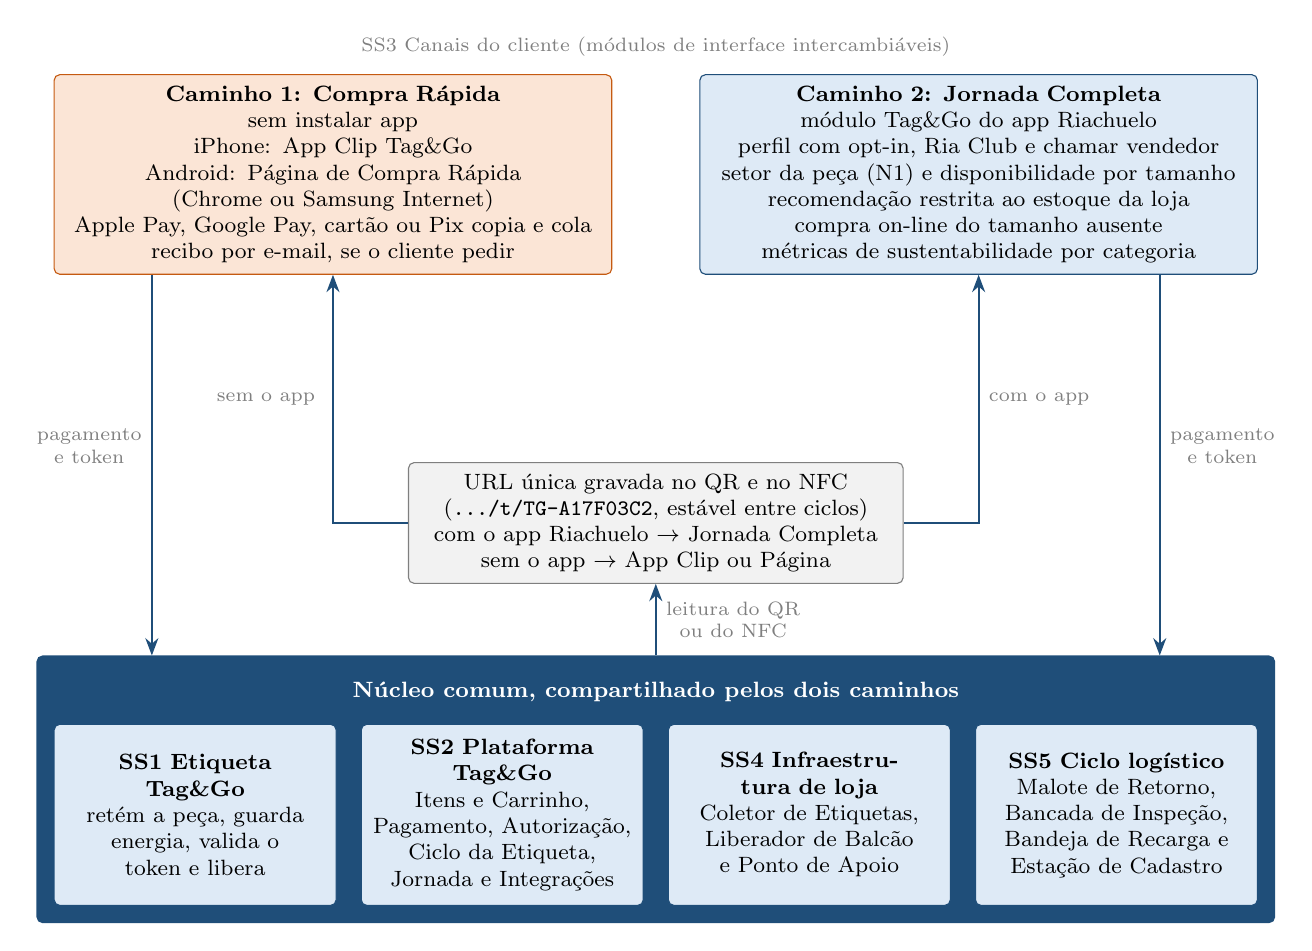
\begin{tikzpicture}
        \node[r2rotulo] (ss3) at (0,6.6) {SS3 Canais do cliente (módulos de interface intercambiáveis)};
        \node[r2destaque, anchor=north, text width=6.8cm] (cr) at (-4.1,6.25) {\textbf{Caminho 1: Compra Rápida}\\ sem instalar app\\ iPhone: App Clip Tag\&Go\\ Android: Página de Compra Rápida\\ (Chrome ou Samsung Internet)\\ Apple Pay, Google Pay, cartão ou Pix copia e cola\\ recibo por e-mail, se o cliente pedir};
        \node[r2bloco, anchor=north, text width=6.8cm] (jc) at (4.1,6.25) {\textbf{Caminho 2: Jornada Completa}\\ módulo Tag\&Go do app Riachuelo\\ perfil com opt-in, Ria Club e chamar vendedor\\ setor da peça (N1) e disponibilidade por tamanho\\ recomendação restrita ao estoque da loja\\ compra on-line do tamanho ausente\\ métricas de sustentabilidade por categoria};
        \node[r2neutro, text width=6.0cm] (url) at (0,0.55) {URL única gravada no QR e no NFC\\ (\texttt{.../t/TG-A17F03C2}, estável entre ciclos)\\ com o app Riachuelo $\rightarrow$ Jornada Completa\\ sem o app $\rightarrow$ App Clip ou Página};
        \node[font=\footnotesize\bfseries, text=white] (tit) at (0,-1.6) {Núcleo comum, compartilhado pelos dois caminhos};
        \node[r2bloco, anchor=north, text width=3.3cm, minimum height=2.3cm] (s1) at (-5.85,-2.0) {\textbf{SS1 Etiqueta Tag\&Go}\\ retém a peça, guarda energia, valida o token e libera};
        \node[r2bloco, anchor=north, text width=3.3cm, minimum height=2.3cm] (s2) at (-1.95,-2.0) {\textbf{SS2 Plataforma Tag\&Go}\\ Itens e Carrinho, Pagamento, Autorização, Ciclo da Etiqueta, Jornada e Integrações};
        \node[r2bloco, anchor=north, text width=3.3cm, minimum height=2.3cm] (s4) at (1.95,-2.0) {\textbf{SS4 Infraestrutura de loja}\\ Coletor de Etiquetas, Liberador de Balcão e Ponto de Apoio};
        \node[r2bloco, anchor=north, text width=3.3cm, minimum height=2.3cm] (s5) at (5.85,-2.0) {\textbf{SS5 Ciclo logístico}\\ Malote de Retorno, Bancada de Inspeção, Bandeja de Recarga e Estação de Cadastro};
        \begin{scope}[on background layer]
            \node[r2blocoescuro, fit=(tit)(s1)(s2)(s4)(s5), inner sep=6pt] (nucleo) {};
        \end{scope}
        \draw[r2seta] (url.west) -| node[r2rotulo, pos=0.75, left] {sem o app} (cr.south);
        \draw[r2seta] (url.east) -| node[r2rotulo, pos=0.75, right] {com o app} (jc.south);
        \coordinate (a1) at ([xshift=-2.3cm]cr.south);
        \coordinate (a2) at ([xshift=2.3cm]jc.south);
        \draw[r2seta] (a1) -- node[r2rotulo, pos=0.45, left] {pagamento\\ e token} (a1 |- nucleo.north);
        \draw[r2seta] (a2) -- node[r2rotulo, pos=0.45, right] {pagamento\\ e token} (a2 |- nucleo.north);
        \draw[r2seta] (url.south |- nucleo.north) -- node[r2rotulo, right] {leitura do QR\\ ou do NFC} (url.south);
    \end{tikzpicture}}
    \source{Elaborado pelos autores (2026).}
\end{figure}

O núcleo comum tem quatro subsistemas. A etiqueta Tag\&Go (SS1) retém a peça, guarda energia, verifica o token e libera o pino, e traz impressos um QR e um NFC com a mesma URL. A Plataforma Tag\&Go (SS2) reúne os serviços Itens e Carrinho, que resolve o identificador da etiqueta em EPC da peça, SKU e preço; Pagamento; Autorização, com a chave mestra guardada num HSM; Ciclo da Etiqueta, que mantém os estados e a frota; Jornada, que concentra perfil, localização, disponibilidade, recomendação, sustentabilidade e consentimento; e Integrações, com o estoque RFID e o OMS, o PDV e a emissão de NFC-e, o Ria Club e o e-commerce. A infraestrutura de loja (SS4) tem o Coletor de Etiquetas, o Liberador de Balcão e o Ponto de Apoio, e o ciclo logístico (SS5) tem o Malote de Retorno, a Bancada de Inspeção, a Bandeja de Recarga e a Estação de Cadastro. Os canais do cliente (SS3) ficam acima do núcleo como módulos intercambiáveis: o App Clip Tag\&Go, a Página de Compra Rápida, o módulo Tag\&Go do app Riachuelo e o passe do Ria Club.

A URL gravada no QR e no NFC contém apenas o identificador público e estável da etiqueta, como \texttt{https://.../t/TG-A17F03C2} (exemplo ilustrativo), e não muda entre ciclos, porque a peça associada em cada ciclo vem da Plataforma. O roteamento depende do aparelho. Um iPhone com o app Riachuelo abre o módulo Tag\&Go, e um iPhone sem o app abre o App Clip Tag\&Go; um Android com o app abre o app por deep link, e um Android sem o app abre a Página de Compra Rápida no navegador \cite{apple2026corenfc,chrome2026webbluetooth}. Um iPhone sem suporte a App Clip abre a página no Safari, que aceita Apple Pay, mas não se comunica com a etiqueta, e nesse caso a liberação acontece no Ponto de Apoio. As duas plataformas precisam ser atendidas desde o início: em agosto de 2026, o Android respondia por 75,45\% e o iOS por 24,54\% do tráfego web móvel no Brasil \cite{statcounter2026so}.

Nos dois caminhos vale a mesma regra de conectividade. A etiqueta não precisa de rede; o celular precisa de dados móveis ou do Wi-Fi de convidados da loja, com acesso livre aos domínios da Plataforma e do PSP (S08), para pagar e obter o token. Sem dados ou sem bateria no celular, a compra segue pelo Liberador de Balcão, que energiza a etiqueta pelos contatos da face superior e recebe o token da Plataforma como dispositivo autenticado (S09). O passo a passo das duas jornadas e os oito cenários de exceção estão na Seção~\ref{sec:r2-arquitetura}.

\subsubsection{Compra Rápida}

A Compra Rápida atende aos autônomos digitais (21\%) e, como via rápida opcional, aos pragmáticos equilibrados (31\%), com foco nas vozes DE01, DE05, D01, D03 e N06. O caminho mostra a peça e o preço, aceita outras peças na mesma compra e aceita pagamento com Apple Pay ou Google Pay, com cartão digitado ou com Pix copia e cola. Na carteira digital, o cliente toca no botão de pagamento e confirma por Face ID, Touch ID ou senha na folha do sistema. Depois do pagamento, o caminho conduz a liberação da etiqueta, envia o recibo por e-mail se o cliente pedir e convida ao Ria Club e ao passe no Wallet. Os dados coletados se limitam ao necessário para pagar e emitir a NFC-e, com CPF na nota opcional, e o e-mail só é pedido quando o cliente quer o recibo.

No iPhone, o canal é o App Clip Tag\&Go, aberto pelo QR ou pelo NFC, com Apple Pay e Core Bluetooth em primeiro plano. A Apple exige que o App Clip tenha um app completo com pelo menos a mesma funcionalidade, no mesmo projeto \cite{apple2026appclipcriar}, de modo que o caminho 1 depende do caminho 2 e do time de iOS da Riachuelo. Com invocação física, o App Clip pode ter até 15\,MB descompactado \cite{apple2026tamanhos} (meta interna de 10\,MB, S04) e não mantém conexão Bluetooth em segundo plano \cite{apple2020forumble}; o cliente precisa, por isso, manter a tela aberta até a luz verde. O ponto mais sensível é o próprio Core Bluetooth: ele não aparece na lista de frameworks indisponíveis em App Clips \cite{apple2026appclipfuncoes}, e no fórum oficial a Apple respondeu que App Clips podem usar Bluetooth \cite{apple2020forumble}. A disponibilidade é uma dedução da documentação, sem confirmação explícita, e tornou-se o primeiro marco de decisão do protótipo no Relatório 3; se o teste falhar, o App Clip continua útil para pagar, e a liberação passa ao Liberador de Balcão.

No Android não há equivalente ao App Clip desde o encerramento do Google Play Instant, em dezembro de 2025 \cite{google2026instant}, e o caminho sem instalação passa pela web. A Página de Compra Rápida roda no Chrome ou no Samsung Internet, que oferecem Web Bluetooth \cite{caniuse2026webbluetooth}; a conexão exige um gesto do usuário e abre um seletor de dispositivos, que a página filtra pelo identificador da etiqueta para mostrar uma única opção \cite{chrome2026webbluetooth}. O Google Pay entra pela biblioteca JavaScript da Google Pay API, sem instalar app \cite{google2026paywebvisao}. O Firefox não tem Web Bluetooth, e a página oferece abrir o mesmo endereço no Chrome; o sistema pode pedir permissão de dispositivos por perto ou de localização no primeiro uso, conforme a versão do Android, atrito que será medido no protótipo.

O Pix copia e cola fica sempre disponível nos dois sistemas, porque 60\% dos brasileiros pesquisados pela Adyen disseram desistir de compras em loja física quando não podem pagar como querem \cite{tiinside2026adyen}. Como o Pix é assíncrono, a luz verde só acende depois da confirmação do pagamento, e o tempo de liquidação fica fora da meta R03. O Pix pelo Google Pay com Open Finance fica pendente até a confirmação do banco e não tem documentação que confirme um fluxo de um clique na web \cite{yuno2026googlepaypix}; a equipe o tratou como hipótese a validar com o PSP.

\subsubsection{Jornada Completa}

A Jornada Completa atende aos frustrados com disponibilidade (9\%), a quem compra para terceiros (N07 e D05), aos dependentes de atendimento (39\%), pelo botão ``chamar vendedor'' (N01, N08 e D04), e aos membros do Ria Club. O público é uma hipótese da equipe: o survey do Relatório 1 não mediu interesse por fidelidade, recomendação ou sustentabilidade, e o apoio a essas funções é qualitativo. Nas entrevistas, Felipe pediu estoque em tempo real, Wagner pediu uma tabela de medidas melhor e Luana citou brechó e privacidade de dados.

O caminho roda como módulo Tag\&Go dentro do app Riachuelo, que já tem mais de 10 milhões de downloads e nota 4,8 com 341 mil avaliações no Google Play \cite{googleplay2026riachuelo}, nota 4,9 com 323 mil avaliações na App Store \cite{appstore2026riachuelo} e integração com cartão, Pix e Ria Club. O app atual não localiza a peça na loja nem mostra estoque por loja, lacunas que o módulo preenche. Para dimensionar o alcance, a equipe usou os 4,5 milhões de clientes ativos do cartão \cite{btg2025guararapes}, e não a carteira histórica da Midway.

O módulo guarda um perfil com tamanhos, preferências e dependentes, com opt-in; mostra o setor e o piso da peça (nível N1) e a disponibilidade por tamanho com leitura RFID de até 24\,h; recomenda peças restritas ao que existe na loja no tamanho do perfil; oferece a compra on-line do tamanho ausente; acumula benefícios do Ria Club; mostra métricas de sustentabilidade por categoria; aciona um vendedor; e permite gerenciar consentimentos. A recomendação seguirá um modelo híbrido, com regras de coleção, filtragem colaborativa, similaridade visual e looks montados por stylists, na linha da Stitch Fix e da Zalando \cite{stitchfix2026algoritmos,zalando2021looks}; a Renner já compara produtos por imagem \cite{infomoney2024renner}.

A compra on-line do tamanho ausente terá retirada na loja sem custo ou entrega sem frete acima de um valor mínimo a definir com a Riachuelo, com R\$~199 como premissa de trabalho. Com frete médio de R\$~18 por pedido, também premissa, um pedido recuperado de R\$~210 (três peças de R\$~70, estimativa da equipe) contribui com cerca de R\$~101, isto é, R\$~119 de margem bruta menos o frete. Essa receita é incremental e não entra no equilíbrio econômico do núcleo calculado na Seção~\ref{sec:r2-valor}.

No Ria Club, o cashback de uma compra pela Jornada Completa só será liberado depois do registro de ``etiqueta devolvida'' no Coletor, o que liga a fidelidade à meta de retorno S01. O regulamento não permite acumular nem resgatar cashback nas lojas do Amazonas, do Pará, do Piauí, de Rondônia e de Santa Catarina \cite{midway2026riaclub}; o módulo tratará essa exceção, e caberá à Riachuelo decidir se a compra feita pelo app dentro da loja conta como compra no app para fins do programa.

As métricas de sustentabilidade serão apresentadas como estimativa por categoria, com faixa e fonte, e nunca como pegada individual da peça. Uma camiseta de algodão, por exemplo, tem mediana de 3,0\,kg CO$_2$e, com faixa de 2,1 a 4,1\,kg CO$_2$e \cite{devera2026camiseta}, e uma calça jeans soma 33,4\,kg CO$_2$e e 3.781\,L de água no ciclo completo \cite{levis2015lca}. O Joint Research Centre considera o cálculo por modelo, com as regras de pegada ambiental de vestuário, a única forma escalável \cite{jrc2026dpp}, e apresentar valores genéricos como pegada da peça pode configurar publicidade enganosa por omissão \cite{brasil1990cdc}.

\subsubsection{Ponte entre os caminhos e comparação}

A Compra Rápida funciona também como porta de entrada para a Jornada Completa. Depois da compra, o cliente pode adicionar o passe do Ria Club ao Apple Wallet ou ao Google Wallet sem instalar o app, e o passe leva ao app quando o cliente quiser \cite{apple2026walletpass,google2026walletfidelidade}. No iPhone, o App Clip recomenda o app completo no fim da tarefa \cite{apple2026appcliphig} e deixa o histórico da compra num espaço compartilhado para o app herdar \cite{apple2026appclipdados}. As notificações efêmeras do App Clip, permitidas por até 8\,h depois de cada abertura \cite{apple2026appclipnotif}, servem ao recibo e a uma pesquisa curta pós-compra, e o Sign in with Apple, oferecido só depois da compra, estende a guarda dos dados do App Clip de 10 para 30 dias \cite{apple2026appclipsuporte}. A comparação completa dos dois caminhos está na Tabela~\ref{tab:r2-caminhos}.

\begin{table}[htbp]
    \centering
    \caption{Comparação entre a Compra Rápida e a Jornada Completa}
    \label{tab:r2-caminhos}
    \footnotesize
    \renewcommand{\arraystretch}{1.25}
    \begin{tabularx}{\textwidth}{@{}
        >{\RaggedRight\arraybackslash}p{2.5cm}
        >{\RaggedRight\arraybackslash}X
        >{\RaggedRight\arraybackslash}X@{}}
        \toprule
        \textbf{Dimensão} & \textbf{Compra Rápida} & \textbf{Jornada Completa} \\
        \midrule
        Público principal & autônomos digitais; pragmáticos equilibrados como via rápida & frustrados com disponibilidade; quem compra para terceiros; membros do Ria Club; dependentes de atendimento, pelo botão ``chamar vendedor'' \\
        Instalação & nenhuma (App Clip no iPhone; página no Android) & app Riachuelo com o módulo Tag\&Go \\
        Como abre & QR ou NFC da etiqueta (mesma URL) & QR ou NFC da etiqueta, ou o próprio app \\
        Pagamento & Apple Pay, Google Pay, cartão, Pix copia e cola & os mesmos meios, mais cartão Riachuelo e Pix no cartão \\
        Funções & núcleo comum, com interface mínima no celular & núcleo comum mais as funções de localização, disponibilidade, recomendação, compra on-line, benefícios, sustentabilidade e consentimento \\
        Dados e base legal & mínimos; execução de contrato; CPF opcional & perfil com opt-in por finalidade; consentimento ou legítimo interesse com teste de balanceamento \\
        Dependências & app Riachuelo publicado com a mesma função (exigência do App Clip); Core Bluetooth no App Clip a validar; Web Bluetooth só no Chrome e no Samsung Internet & integrações com estoque RFID, OMS e Ria Club; planograma mantido pela loja \\
        Limitações & App Clip de até 15\,MB e sem segundo plano; Pix assíncrono; permissões no primeiro uso & adesão depende do app; Ria Club não vale em 5 estados \\
        Métrica de sucesso & R03, R04, R05 & R01, R02, conversão da recomendação, adesão ao Ria Club, pedidos on-line recuperados \\
        \bottomrule
    \end{tabularx}
    \source{Elaborado pelos autores (2026) com base em \citeonline{apple2026appclipcriar}, \citeonline{apple2026tamanhos}, \citeonline{caniuse2026webbluetooth}, \citeonline{brasil2018lgpd} e \citeonline{midway2026riaclub}.}
\end{table}

A equipe concluiu, a partir da comparação, que os dois caminhos se completam: a Compra Rápida responde pelos requisitos de tempo, autonomia e clareza (R03, R04 e R05), que somam 51,3\% da importância técnica no QFD; a Jornada Completa, pelos de localização e disponibilidade (R01 e R02); e o núcleo comum garante nos dois caminhos a liberação condicionada ao pagamento (R06). As bases legais diferem porque as finalidades diferem, e perfil e preferências exigem opt-in separado por finalidade \cite{brasil2018lgpd}; o tratamento dos dados pessoais está na Seção~\ref{sec:r2-comercializacao}.

\subsection{Organização do relatório}
\label{sub:r2-organizacao}

As seções seguintes seguem os seis itens do roteiro das Aulas 12 e 13 \cite{zancul2026conceitual}, com a reformulação dos desenhos dividida em duas seções: uma para os princípios de solução e a escolha da concepção e outra para a arquitetura e os desenhos. A ordem acompanha a dependência entre os itens: a análise funcional define o que o sistema precisa fazer; a diferenciação, a escala vertical e o aproveitamento técnico reúnem as referências que alimentam a matriz morfológica; a concepção escolhida é detalhada na arquitetura; e a comercialização fecha o conceito. A correspondência entre os itens do roteiro, as seções e as figuras e tabelas está na Tabela~\ref{tab:r2-roteiro}.

\begin{table}[htbp]
    \centering
    \caption{Correspondência entre os itens do roteiro e as seções do relatório}
    \label{tab:r2-roteiro}
    \footnotesize
    \renewcommand{\arraystretch}{1.25}
    \begin{tabularx}{\textwidth}{@{}
        >{\RaggedRight\arraybackslash}p{6.2cm}
        c
        >{\RaggedRight\arraybackslash}X@{}}
        \toprule
        \textbf{Item do roteiro (Aulas 12 e 13)} & \textbf{Seção} & \textbf{Figuras e tabelas} \\
        \midrule
        Contexto e especificações-meta (correção do Relatório 1) & \ref{sec:r2-contexto} & Figura~\ref{fig:r2-caminhos}; Tabelas~\ref{tab:r2-especificacoes}, \ref{tab:r2-caminhos} e \ref{tab:r2-roteiro} \\
        A. Análise funcional: funções principais e secundárias & \ref{sec:r2-funcional} & Figuras~\ref{fig:r2-caixapreta}, \ref{fig:r2-ef-alternativas} e \ref{fig:r2-ef-escolhida}; Tabelas~\ref{tab:r2-funcoes}, \ref{tab:r2-granularidade} e \ref{tab:r2-estruturas} \\
        B. Estudo de diferenciação & \ref{sec:r2-diferenciacao} & Figura~\ref{fig:r2-posicionamento}; Tabela~\ref{tab:r2-diferenciacao} \\
        C. Escala vertical e valor mercadológico & \ref{sec:r2-valor} & Figuras~\ref{fig:r2-escala-vertical}, \ref{fig:r2-custo-uso}, \ref{fig:r2-equilibrio} e \ref{fig:r2-tornado}; Tabelas~\ref{tab:r2-escala}, \ref{tab:r2-bom} e \ref{tab:r2-valor} \\
        D. Estudo de aproveitamento técnico & \ref{sec:r2-aproveitamento} & Tabela~\ref{tab:r2-aproveitamento} \\
        E. Reformulação dos desenhos (parte 1: princípios de solução e concepção) & \ref{sec:r2-concepcao} & Figura~\ref{fig:r2-sensibilidade-matriz}; Tabelas~\ref{tab:r2-efeitos}, \ref{tab:r2-morfologica} e \ref{tab:r2-decisao} \\
        E. Reformulação dos desenhos (parte 2: arquitetura e desenhos) & \ref{sec:r2-arquitetura} & Figuras~\ref{fig:r2-arquitetura}, \ref{fig:r2-desenho}, \ref{fig:r2-fluxo-rapida}, \ref{fig:r2-fluxo-completa}, \ref{fig:r2-ciclo} e \ref{fig:r2-frota}; Tabelas~\ref{tab:r2-ssc}, \ref{tab:r2-interfaces}, \ref{tab:r2-mudancas} e \ref{tab:r2-ameacas} \\
        F. Delineamento da comercialização e da distribuição & \ref{sec:r2-comercializacao} & Figura~\ref{fig:r2-cronograma}; Tabelas~\ref{tab:r2-canais}, \ref{tab:r2-lgpd} e \ref{tab:r2-riscos} \\
        Considerações finais & \ref{sec:r2-consideracoes} & nenhuma \\
        \bottomrule
    \end{tabularx}
    \source{Elaborado pelos autores (2026) com base em \citeonline{zancul2026conceitual}.}
\end{table}

\newpage% =============================================================================
% Relatorio 2, Secao 2: analise funcional (item A do roteiro).
% Metodo: funcao global, caixa-preta com fluxos de energia, material e sinal,
% duas estruturas funcionais alternativas (EF-1 e EF-2), escolha da estrutura
% mista (EF-M) e lista de 31 funcoes classificadas (F1 a F31, alem de F0).
% Figuras: fig:r2-caixapreta, fig:r2-ef-alternativas, fig:r2-ef-escolhida.
% Tabelas: tab:r2-estruturas, tab:r2-funcoes, tab:r2-granularidade.
% Principios de solucao ficam na Secao 6 (r2/8-concepcao.tex); precos, na
% Secao 4 (r2/6-escala-valor.tex).
% =============================================================================

\section{ANÁLISE FUNCIONAL}
\label{sec:r2-funcional}

Com as especificações-meta fixadas e os dois caminhos definidos, a equipe passou a decompor o que o sistema precisa fazer. A análise funcional seguiu o método de \citeonline{rozenfeld2006gestao}, na forma apresentada nas aulas de projeto conceitual da disciplina \cite{zancul2026conceitual}. A equipe partiu da função global do sistema Tag\&Go, representou-a como caixa-preta com os fluxos de energia (E), material (M) e sinal (S) que atravessam a fronteira do sistema, montou duas estruturas funcionais alternativas, comparou-as por uma matriz simples de avaliação e desdobrou a estrutura escolhida em uma lista de funções classificadas. Cada função foi escrita como verbo mais substantivo e descreve o que o sistema deve fazer, sem antecipar como. Por essa regra, a luz da etiqueta cumpre a função de indicar o estado da liberação, e a leitura RFID na loja serve à função de registrar a venda no estoque; luz e RFID são portadores de solução, escolhidos com a matriz morfológica na Seção~\ref{sec:r2-concepcao}.

A orientação da disciplina para esta fase foi considerar todas as funções necessárias, inclusive as que a equipe não pretende realizar no protótipo, porque uma função omitida agora exclui do produto a possibilidade de executá-la depois \cite{zancul2026conceitual}. Por isso, a lista inclui as funções do ciclo logístico da etiqueta e as da Jornada Completa, que o Relatório 1 havia deixado implícitas, e a simplificação ficará restrita ao protótipo, a ser delimitado no Relatório 3. As funções valem para os dois caminhos de uso apresentados na Seção~\ref{sec:r2-contexto} (Figura~\ref{fig:r2-caminhos}): o núcleo comum reúne as funções sem as quais a compra não se completa, e a Jornada Completa acrescenta, no módulo Tag\&Go do app Riachuelo, funções de apoio à escolha e à fidelização; na Compra Rápida, o cliente cumpre as funções do núcleo sem instalar aplicativo.

\subsection{Função global e caixa-preta}
\label{sub:r2-caixapreta}

A equipe definiu a função global do sistema como liberar peça mediante pagamento (F0). A formulação reúne as duas condições que cliente e varejista esperam do produto: para o cliente, sair com a peça sem passar pelo caixa; para o varejista, garantir que nenhuma peça deixe a loja sem pagamento confirmado, condição expressa no requisito R06, que concentrou 33,1\% da importância técnica no Relatório 1. A função global não menciona etiqueta, celular nem aplicativo, porque esses elementos já são escolhas de solução.

A fronteira delimita o que a equipe projeta. Dentro dela estão os cinco subsistemas do Tag\&Go: a etiqueta (SS1), a Plataforma Tag\&Go e seus serviços (SS2), os canais do cliente (SS3), a infraestrutura de loja (SS4) e o ciclo logístico (SS5), detalhados na Seção~\ref{sec:r2-arquitetura} (Tabela~\ref{tab:r2-ssc}). Fora dela ficam os elementos com que o sistema troca fluxos e que a Riachuelo ou terceiros já operam: o cliente e o celular dele, o funcionário da loja, o provedor de pagamento (PSP) e as carteiras digitais, o estoque RFID e o sistema de gestão de pedidos (OMS), o PDV e o emissor de NFC-e, os pórticos EAS e RFID, o app Riachuelo e o Ria Club. A Figura~\ref{fig:r2-caixapreta} mostra a caixa-preta resultante.

\begin{figure}[htbp]
    \centering
    \caption{Caixa-preta da função global}
    \label{fig:r2-caixapreta}
    \resizebox{\textwidth}{!}{%
    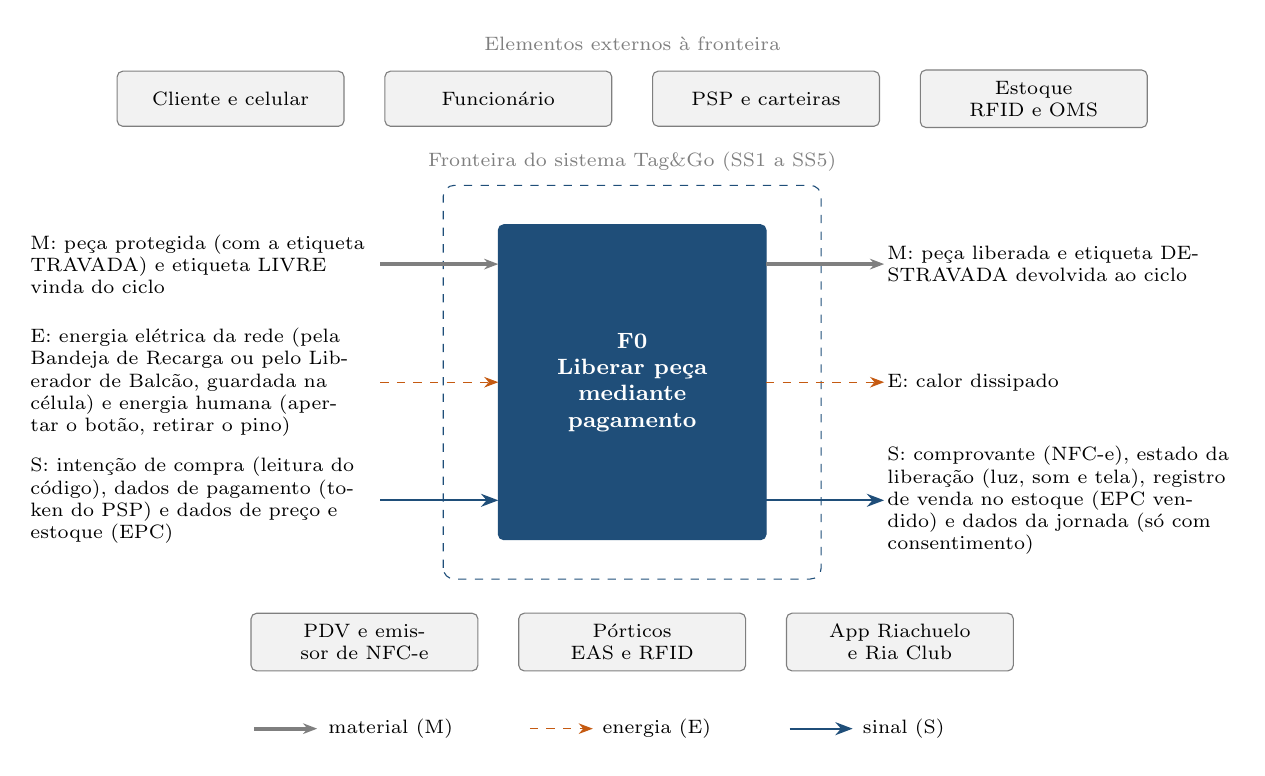
\begin{tikzpicture}[
        ent/.style={font=\scriptsize, align=left, text width=4.4cm, inner sep=1pt},
        mat/.style={r2setafina, line width=1.4pt},
        ext/.style={r2neutro, font=\scriptsize, text width=2.6cm, minimum height=7mm}
    ]
        % fronteira do sistema
        \draw[r2azul, dashed, rounded corners=4pt] (-2.4,-2.5) rectangle (2.4,2.5);
        \node[r2rotulo, anchor=south] at (0,2.55) {Fronteira do sistema Tag\&Go (SS1 a SS5)};
        \node[r2blocoescuro, text width=3.0cm, minimum width=3.4cm, minimum height=4cm] (f0) at (0,0) {F0\\Liberar peça\\mediante pagamento};
        % entradas
        \node[ent, anchor=east] at (-3.2,1.5) {M: peça protegida (com a etiqueta TRAVADA) e etiqueta LIVRE vinda do ciclo};
        \node[ent, anchor=east] at (-3.2,0) {E: energia elétrica da rede (pela Bandeja de Recarga ou pelo Liberador de Balcão, guardada na célula) e energia humana (apertar o botão, retirar o pino)};
        \node[ent, anchor=east] at (-3.2,-1.5) {S: intenção de compra (leitura do código), dados de pagamento (token do PSP) e dados de preço e estoque (EPC)};
        \draw[mat] (-3.2,1.5) -- (-1.7,1.5);
        \draw[r2setatracejada] (-3.2,0) -- (-1.7,0);
        \draw[r2seta] (-3.2,-1.5) -- (-1.7,-1.5);
        % saidas
        \draw[mat] (1.7,1.5) -- (3.2,1.5);
        \draw[r2setatracejada] (1.7,0) -- (3.2,0);
        \draw[r2seta] (1.7,-1.5) -- (3.2,-1.5);
        \node[ent, anchor=west] at (3.2,1.5) {M: peça liberada e etiqueta DESTRAVADA devolvida ao ciclo};
        \node[ent, anchor=west] at (3.2,0) {E: calor dissipado};
        \node[ent, anchor=west] at (3.2,-1.5) {S: comprovante (NFC-e), estado da liberação (luz, som e tela), registro de venda no estoque (EPC vendido) e dados da jornada (só com consentimento)};
        % elementos externos
        \node[r2rotulo] at (0,4.3) {Elementos externos à fronteira};
        \node[ext] at (-5.1,3.6) {Cliente e celular};
        \node[ext] at (-1.7,3.6) {Funcionário};
        \node[ext] at (1.7,3.6) {PSP e carteiras};
        \node[ext] at (5.1,3.6) {Estoque RFID e OMS};
        \node[ext] at (-3.4,-3.3) {PDV e emissor de NFC-e};
        \node[ext] at (0,-3.3) {Pórticos EAS e RFID};
        \node[ext] at (3.4,-3.3) {App Riachuelo e Ria Club};
        % legenda
        \draw[mat] (-4.8,-4.4) -- (-4.0,-4.4) node[right, font=\scriptsize] {material (M)};
        \draw[r2setatracejada] (-1.3,-4.4) -- (-0.5,-4.4) node[right, font=\scriptsize] {energia (E)};
        \draw[r2seta] (2.0,-4.4) -- (2.8,-4.4) node[right, font=\scriptsize] {sinal (S)};
    \end{tikzpicture}%
    }
    \source{Elaborado pelos autores (2026).}
\end{figure}

As entradas de material são a peça protegida, isto é, a peça com a etiqueta no estado TRAVADA, e a etiqueta no estado LIVRE que volta do ciclo logístico para ser fixada em nova peça. A energia entra por dois caminhos: a energia elétrica da rede, que chega à etiqueta pela Bandeja de Recarga no CD ou pelo Liberador de Balcão na loja e fica guardada na célula, e a energia humana do cliente, que aperta o botão e retira o pino. Os sinais de entrada são a intenção de compra, expressa na leitura do código da etiqueta, os dados de pagamento, que chegam como token do PSP, e os dados de preço e estoque, associados ao EPC da peça. Na saída, o material é a peça liberada e a etiqueta no estado DESTRAVADA, devolvida ao ciclo; a energia deixa o sistema como calor; e os sinais são o comprovante fiscal (NFC-e), o estado da liberação, comunicado por luz, som e tela, o registro de venda no estoque (EPC marcado como vendido) e, só com o consentimento do cliente, os dados da jornada.

Dois pontos da caixa-preta orientaram o restante da análise. O primeiro é que a etiqueta aparece ao mesmo tempo como entrada e como saída de material, o que faz do produto um ativo retornável e exige funções de recolhimento, transporte, inspeção e recarga, reunidas no ciclo da etiqueta (Subseção~\ref{sub:r2-funcoes-ciclo}). O segundo é o registro de venda no estoque, saída de sinal que fecha a malha antifraude: como o pórtico RFID da loja alarma quando passa um EPC não vendido, a baixa da peça precisa ocorrer antes de o cliente chegar à saída, o que a especificação S07 fixa em até 5\,s após a confirmação do pagamento (Tabela~\ref{tab:r2-especificacoes}).

\subsection{Estruturas funcionais alternativas}
\label{sub:r2-ef-alternativas}

A partir da caixa-preta, a equipe montou duas estruturas funcionais que diferem no lugar onde a autorização encontra a peça, representadas na Figura~\ref{fig:r2-ef-alternativas}. Na EF-1, liberação na peça, o sinal de autorização viaja até a peça, que permanece com o cliente em qualquer ponto da loja; as funções de validar a autorização (F5), confirmar a intenção de liberar (F10), desfazer a retenção (F6) e indicar o estado ficam junto da peça, e a energia necessária para executá-las viaja com ela (F7). Na EF-2, liberação em ponto fixo, o cliente leva a peça até um ponto da loja onde já existem energia e sinal; a validação e a liberação acontecem nesse ponto, e a etiqueta se limita a reter a peça e a identificá-la.

\begin{figure}[htbp]
    \centering
    \caption{Estruturas funcionais alternativas}
    \label{fig:r2-ef-alternativas}
    \begin{subfigure}{0.48\textwidth}
        \centering
        \caption{EF-1, liberação na peça}
        \resizebox{\linewidth}{!}{%
        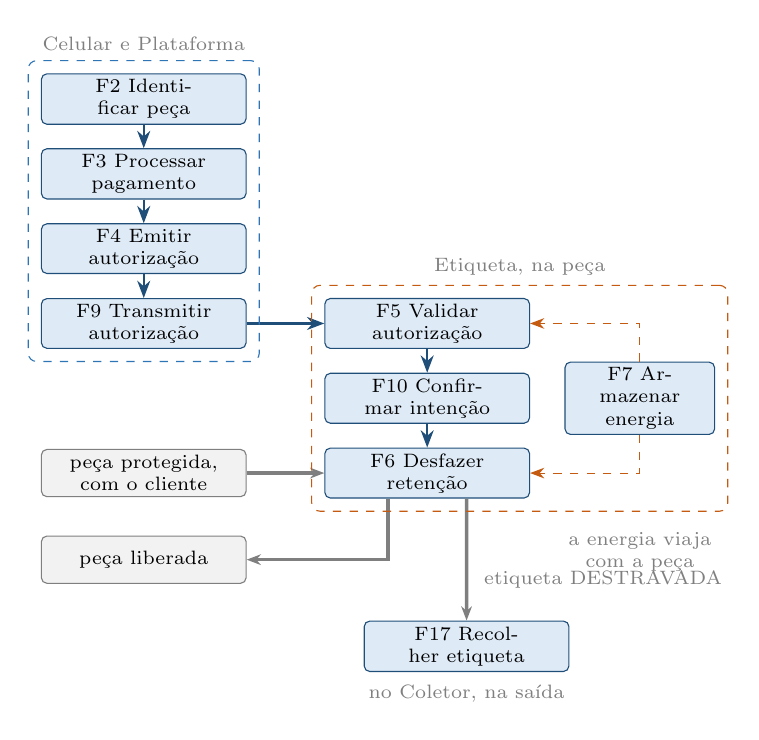
\begin{tikzpicture}[
            bl/.style={r2bloco, font=\scriptsize, text width=2.3cm, minimum width=2.6cm, minimum height=6mm, inner sep=2pt},
            nt/.style={r2neutro, font=\scriptsize, text width=2.3cm, minimum width=2.6cm, minimum height=6mm, inner sep=2pt},
            mat/.style={r2setafina, line width=1.3pt}
        ]
            \node[bl] (f2) at (0,0) {F2 Identificar peça};
            \node[bl] (f3) at (0,-0.95) {F3 Processar pagamento};
            \node[bl] (f4) at (0,-1.9) {F4 Emitir autorização};
            \node[bl] (f9) at (0,-2.85) {F9 Transmitir autorização};
            \node[bl] (f5) at (3.6,-2.85) {F5 Validar autorização};
            \node[bl] (f10) at (3.6,-3.8) {F10 Confirmar intenção};
            \node[bl] (f6) at (3.6,-4.75) {F6 Desfazer retenção};
            \node[bl, text width=1.6cm, minimum width=1.9cm] (f7) at (6.3,-3.8) {F7 Armazenar energia};
            \node[nt] (pm1) at (0,-4.75) {peça protegida, com o cliente};
            \node[nt] (pm2) at (0,-5.85) {peça liberada};
            \node[bl] (f17) at (4.1,-6.95) {F17 Recolher etiqueta};
            \draw[r2seta] (f2) -- (f3);
            \draw[r2seta] (f3) -- (f4);
            \draw[r2seta] (f4) -- (f9);
            \draw[r2seta] (f9) -- (f5);
            \draw[r2seta] (f5) -- (f10);
            \draw[r2seta] (f10) -- (f6);
            \draw[r2setatracejada] (f7.north) |- (f5.east);
            \draw[r2setatracejada] (f7.south) |- (f6.east);
            \draw[mat] (pm1) -- (f6);
            \draw[mat] ([xshift=-5mm]f6.south) |- (pm2.east);
            \draw[mat] ([xshift=5mm]f6.south) -- (f17.north);
            \node[r2rotulo, anchor=west] at (4.2,-6.1) {etiqueta DESTRAVADA};
            \node[r2rotulo] at (6.3,-5.75) {a energia viaja\\com a peça};
            \node[r2rotulo] at (4.1,-7.55) {no Coletor, na saída};
            \node[draw=r2azulmedio, dashed, rounded corners=3pt, inner sep=1.6mm, fit=(f2)(f9), label={[r2rotulo]above:{Celular e Plataforma}}] {};
            \node[draw=r2laranja, dashed, rounded corners=3pt, inner sep=1.6mm, fit=(f5)(f6)(f7), label={[r2rotulo]above:{Etiqueta, na peça}}] {};
        \end{tikzpicture}%
        }
    \end{subfigure}
    \hfill
    \begin{subfigure}{0.48\textwidth}
        \centering
        \caption{EF-2, liberação em ponto fixo}
        \resizebox{\linewidth}{!}{%
        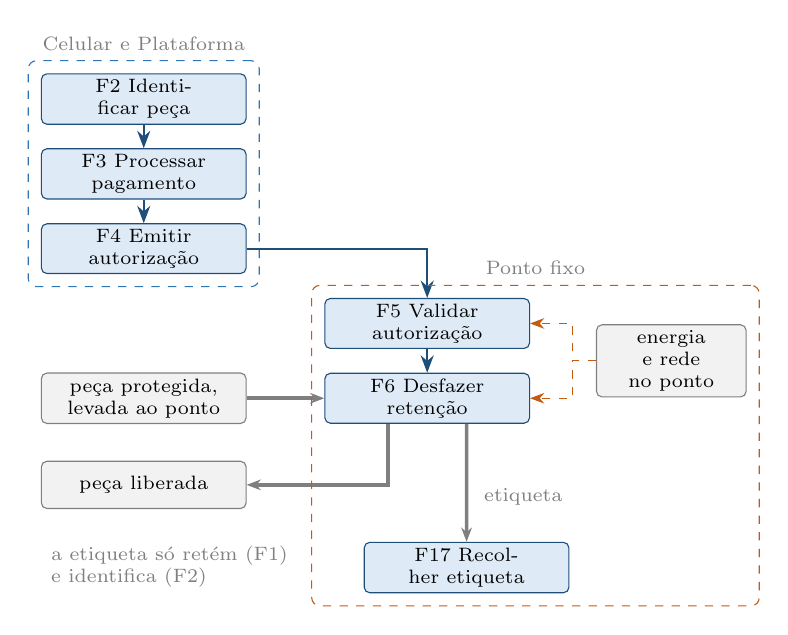
\begin{tikzpicture}[
            bl/.style={r2bloco, font=\scriptsize, text width=2.3cm, minimum width=2.6cm, minimum height=6mm, inner sep=2pt},
            nt/.style={r2neutro, font=\scriptsize, text width=2.3cm, minimum width=2.6cm, minimum height=6mm, inner sep=2pt},
            mat/.style={r2setafina, line width=1.3pt}
        ]
            \node[bl] (f2) at (0,0) {F2 Identificar peça};
            \node[bl] (f3) at (0,-0.95) {F3 Processar pagamento};
            \node[bl] (f4) at (0,-1.9) {F4 Emitir autorização};
            \node[bl] (f5) at (3.6,-2.85) {F5 Validar autorização};
            \node[bl] (f6) at (3.6,-3.8) {F6 Desfazer retenção};
            \node[nt, text width=1.6cm, minimum width=1.9cm] (en) at (6.7,-3.325) {energia e rede no ponto};
            \node[nt] (pm1) at (0,-3.8) {peça protegida, levada ao ponto};
            \node[nt] (pm2) at (0,-4.9) {peça liberada};
            \node[bl] (f17) at (4.1,-5.95) {F17 Recolher etiqueta};
            \draw[r2seta] (f2) -- (f3);
            \draw[r2seta] (f3) -- (f4);
            \draw[r2seta] (f4.east) -| (f5.north);
            \draw[r2seta] (f5) -- (f6);
            \draw[r2setatracejada] (en.west) -- ++(-0.3,0) |- (f5.east);
            \draw[r2setatracejada] (en.west) -- ++(-0.3,0) |- (f6.east);
            \draw[mat] (pm1) -- (f6);
            \draw[mat] ([xshift=-5mm]f6.south) |- (pm2.east);
            \draw[mat] ([xshift=5mm]f6.south) -- (f17.north);
            \node[r2rotulo, anchor=west] at (4.2,-5.05) {etiqueta};
            \node[r2rotulo, align=left, anchor=north west] at (-1.3,-5.55) {a etiqueta só retém (F1)\\e identifica (F2)};
            \node[draw=r2azulmedio, dashed, rounded corners=3pt, inner sep=1.6mm, fit=(f2)(f4), label={[r2rotulo]above:{Celular e Plataforma}}] {};
            \node[draw=r2laranja, dashed, rounded corners=3pt, inner sep=1.6mm, fit=(f5)(f6)(en)(f17), label={[r2rotulo]above:{Ponto fixo}}] {};
        \end{tikzpicture}%
        }
    \end{subfigure}

    \medskip
    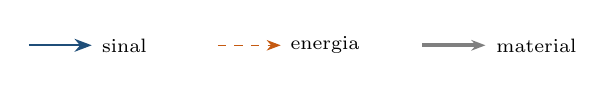
\begin{tikzpicture}[mat/.style={r2setafina, line width=1.3pt}]
        \draw[r2seta] (0,0) -- (0.8,0) node[right, font=\scriptsize] {sinal};
        \draw[r2setatracejada] (2.4,0) -- (3.2,0) node[right, font=\scriptsize] {energia};
        \draw[mat] (5.0,0) -- (5.8,0) node[right, font=\scriptsize] {material};
    \end{tikzpicture}
    \source{Elaborado pelos autores (2026).}
\end{figure}

A comparação usou quatro requisitos do Relatório 1 e dois critérios de viabilidade, o custo e a complexidade da estrutura e a dependência de infraestrutura fixa na loja, com uma escala qualitativa de três níveis: $++$ para muito favorável, $+$ para favorável e $-$ para desfavorável. Por se tratar de uma escolha entre estruturas, e não entre concepções, a equipe não atribuiu pesos numéricos aos critérios; a matriz de decisão ponderada ficou reservada às alternativas de concepção, na Seção~\ref{sec:r2-concepcao}. O resultado está na Tabela~\ref{tab:r2-estruturas}.

\begin{table}[htbp]
    \centering
    \caption{Comparação das estruturas funcionais alternativas}
    \label{tab:r2-estruturas}
    \footnotesize
    \renewcommand{\arraystretch}{1.25}
    \begin{tabularx}{\textwidth}{@{}
        >{\RaggedRight\arraybackslash}p{3.8cm}
        >{\RaggedRight\arraybackslash}X
        >{\RaggedRight\arraybackslash}X
        >{\RaggedRight\arraybackslash}X@{}}
        \toprule
        \textbf{Critério} & \textbf{EF-1, liberação na peça} & \textbf{EF-2, liberação em ponto fixo} & \cellcolor{r2laranjaclaro}\textbf{EF-M, estrutura mista} \\
        \midrule
        R03 tempo de pagamento, sem deslocamento nem fila & $++$ & $-$ & \cellcolor{r2laranjaclaro}$++$ \\
        R04 compra sem funcionário & $++$ & $+$ & \cellcolor{r2laranjaclaro}$++$ \\
        R06 liberação condicionada ao pagamento & $+$ (depende só da etiqueta) & $+$ (depende só do ponto) & \cellcolor{r2laranjaclaro}$++$ (dois caminhos com a mesma autorização) \\
        R07 alternativa humana para 100\% das falhas & $-$ (sem caminho quando a etiqueta ou o celular falham) & $++$ & \cellcolor{r2laranjaclaro}$++$ \\
        Custo e complexidade & $-$ (energia em cada etiqueta) & $++$ & \cellcolor{r2laranjaclaro}$-$ \\
        Dependência de infraestrutura fixa & $++$ & $-$ & \cellcolor{r2laranjaclaro}$+$ \\
        \midrule
        Resultado & reprovada em R07 (meta de 100\%) & fraca em R03 e R04, que somaram 37,6\% da importância técnica no Relatório 1 & \cellcolor{r2laranjaclaro}escolhida \\
        \bottomrule
    \end{tabularx}
    \source{Elaborado pelos autores (2026). Escala: $++$ muito favorável; $+$ favorável; $-$ desfavorável.}
\end{table}

A EF-1 atende melhor ao tempo de pagamento (R03) e à compra sem funcionário (R04), porque elimina o deslocamento até um ponto e a fila que pode se formar nele. Ela não oferece, porém, caminho algum quando a etiqueta ou o celular falham: sem energia na etiqueta ou sem bateria no celular, a peça não sai. Essa lacuna reprova a EF-1 em R07, cuja meta é oferecer alternativa humana em 100\% dos cenários de falha catalogados. A EF-2 trata as falhas com facilidade, já que o ponto fixo tem energia e pode ter um funcionário ao lado, e custa menos, porque a etiqueta dispensa eletrônica própria. Em contrapartida, reintroduz o deslocamento e a possibilidade de fila e fica fraca nos requisitos que motivaram o projeto, R03 e R04, que somaram 37,6\% da importância técnica no Relatório 1.

Diante desse conflito, a equipe escolheu uma estrutura mista, a EF-M, que usa a EF-1 no fluxo principal e a EF-2 como caminho assistido para todas as falhas. O ponto fixo da EF-M é o Ponto de Apoio, balcão com funcionário onde fica um Liberador de Balcão, e as duas vias usam a mesma autorização, o que leva R06 ao nível máximo: a etiqueta só abre com uma autorização válida, venha ela pelo celular do cliente ou pelo Liberador. A escolha tem um preço, porque a EF-M herda da EF-1 o custo e a complexidade de ter energia e verificação em cada etiqueta e mantém alguma infraestrutura fixa, ainda que restrita às exceções. A viabilidade econômica dessa decisão é examinada na Seção~\ref{sec:r2-valor}, e os oito cenários de exceção que o caminho assistido cobre (X1 a X8) estão detalhados na Seção~\ref{sec:r2-arquitetura}.

\subsection{Estrutura funcional escolhida}
\label{sub:r2-ef-escolhida}

A Figura~\ref{fig:r2-ef-escolhida} apresenta a EF-M desdobrada em sete grupos de funções: Compra, Autorização, Liberação, Saída, Exceções, Ciclo da etiqueta e Jornada Completa. As funções básicas aparecem em azul-escuro, as secundárias em azul-claro, e a localização do produto na loja (F25), única função marcada como removível, em cinza.

\begin{figure}[htbp]
    \centering
    \caption{Estrutura funcional escolhida (EF-M)}
    \label{fig:r2-ef-escolhida}
    \resizebox{\textwidth}{!}{%
    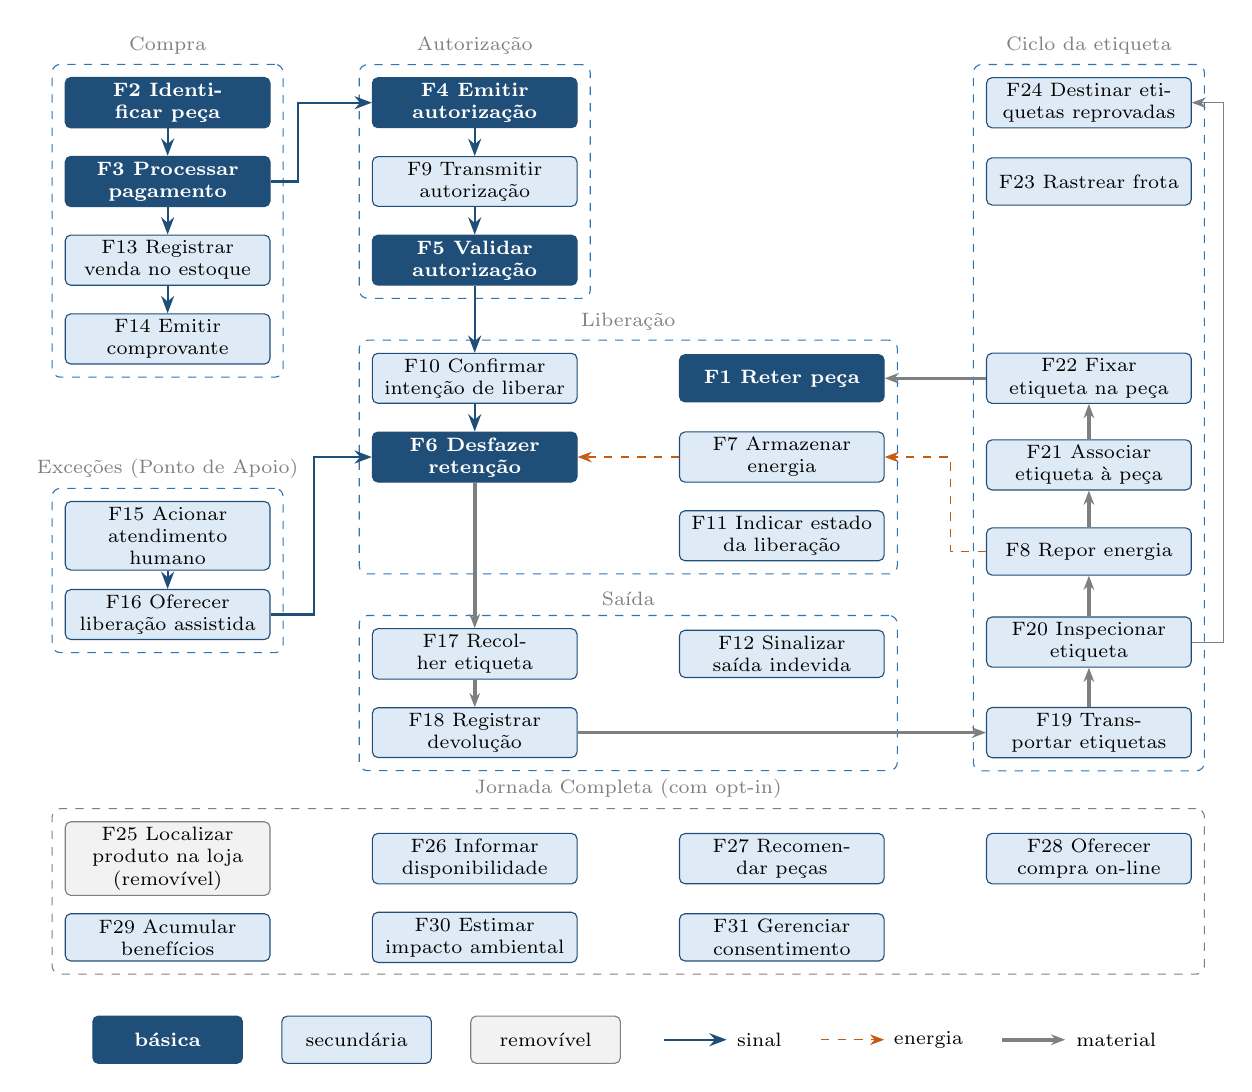
\begin{tikzpicture}[
        fb/.style={r2bloco, font=\scriptsize, text width=2.3cm, minimum width=2.6cm, minimum height=6mm, inner sep=2pt},
        fbb/.style={r2blocoescuro, font=\scriptsize\bfseries, text width=2.3cm, minimum width=2.6cm, minimum height=6mm, inner sep=2pt},
        fbn/.style={r2neutro, font=\scriptsize, text width=2.3cm, minimum width=2.6cm, minimum height=6mm, inner sep=2pt},
        grp/.style={draw=r2azulmedio, dashed, rounded corners=3pt, inner sep=1.6mm},
        mat/.style={r2setafina, line width=1.3pt}
    ]
        % Compra (coluna A)
        \node[fbb] (f2) at (0,0) {F2 Identificar peça};
        \node[fbb] (f3) at (0,-1.0) {F3 Processar pagamento};
        \node[fb] (f13) at (0,-2.0) {F13 Registrar venda no estoque};
        \node[fb] (f14) at (0,-3.0) {F14 Emitir comprovante};
        % Excecoes (coluna A)
        \node[fb] (f15) at (0,-5.5) {F15 Acionar atendimento humano};
        \node[fb] (f16) at (0,-6.5) {F16 Oferecer liberação assistida};
        % Autorizacao (coluna B)
        \node[fbb] (f4) at (3.9,0) {F4 Emitir autorização};
        \node[fb] (f9) at (3.9,-1.0) {F9 Transmitir autorização};
        \node[fbb] (f5) at (3.9,-2.0) {F5 Validar autorização};
        % Liberacao (colunas B e C)
        \node[fb] (f10) at (3.9,-3.5) {F10 Confirmar intenção de liberar};
        \node[fbb] (f6) at (3.9,-4.5) {F6 Desfazer retenção};
        \node[fbb] (f1) at (7.8,-3.5) {F1 Reter peça};
        \node[fb] (f7) at (7.8,-4.5) {F7 Armazenar energia};
        \node[fb] (f11) at (7.8,-5.5) {F11 Indicar estado da liberação};
        % Saida (colunas B e C)
        \node[fb] (f17) at (3.9,-7.0) {F17 Recolher etiqueta};
        \node[fb] (f18) at (3.9,-8.0) {F18 Registrar devolução};
        \node[fb] (f12) at (7.8,-7.0) {F12 Sinalizar saída indevida};
        % Ciclo da etiqueta (coluna D)
        \node[fb] (f24) at (11.7,0) {F24 Destinar etiquetas reprovadas};
        \node[fb] (f23) at (11.7,-1.0) {F23 Rastrear frota};
        \node[fb] (f22) at (11.7,-3.5) {F22 Fixar etiqueta na peça};
        \node[fb] (f21) at (11.7,-4.6) {F21 Associar etiqueta à peça};
        \node[fb] (f8) at (11.7,-5.7) {F8 Repor energia};
        \node[fb] (f20) at (11.7,-6.85) {F20 Inspecionar etiqueta};
        \node[fb] (f19) at (11.7,-8.0) {F19 Transportar etiquetas};
        % Jornada Completa
        \node[fbn] (f25) at (0,-9.6) {F25 Localizar produto na loja (removível)};
        \node[fb] (f26) at (3.9,-9.6) {F26 Informar disponibilidade};
        \node[fb] (f27) at (7.8,-9.6) {F27 Recomendar peças};
        \node[fb] (f28) at (11.7,-9.6) {F28 Oferecer compra on-line};
        \node[fb] (f29) at (0,-10.6) {F29 Acumular benefícios};
        \node[fb] (f30) at (3.9,-10.6) {F30 Estimar impacto ambiental};
        \node[fb] (f31) at (7.8,-10.6) {F31 Gerenciar consentimento};
        % grupos
        \node[grp, fit=(f2)(f14), label={[r2rotulo]above:{Compra}}] {};
        \node[grp, fit=(f4)(f5), label={[r2rotulo]above:{Autorização}}] {};
        \node[grp, fit=(f10)(f6)(f1)(f7)(f11), label={[r2rotulo]above:{Liberação}}] {};
        \node[grp, fit=(f17)(f18)(f12), label={[r2rotulo]above:{Saída}}] {};
        \node[grp, fit=(f15)(f16), label={[r2rotulo]above:{Exceções (Ponto de Apoio)}}] {};
        \node[grp, fit=(f24)(f19), label={[r2rotulo]above:{Ciclo da etiqueta}}] {};
        \node[grp, draw=r2cinza, fit=(f25)(f28)(f31), label={[r2rotulo]above:{Jornada Completa (com opt-in)}}] {};
        % fluxos de sinal
        \draw[r2seta] (f2) -- (f3);
        \draw[r2seta] (f3) -- (f13);
        \draw[r2seta] (f13) -- (f14);
        \draw[r2seta] (f3.east) -- ++(0.35,0) |- (f4.west);
        \draw[r2seta] (f4) -- (f9);
        \draw[r2seta] (f9) -- (f5);
        \draw[r2seta] (f5) -- (f10);
        \draw[r2seta] (f10) -- (f6);
        \draw[r2seta] (f15) -- (f16);
        \draw[r2seta] (f16.east) -- ++(0.55,0) |- (f6.west);
        % fluxos de energia
        \draw[r2setatracejada] (f7.west) -- (f6.east);
        \draw[r2setatracejada] (f8.west) -- ++(-0.45,0) |- (f7.east);
        % fluxos de material
        \draw[mat] (f6) -- (f17);
        \draw[mat] (f17) -- (f18);
        \draw[mat] (f18) -- (f19);
        \draw[mat] (f19) -- (f20);
        \draw[mat] (f20) -- (f8);
        \draw[mat] (f8) -- (f21);
        \draw[mat] (f21) -- (f22);
        \draw[mat] (f22.west) -- (f1.east);
        \draw[r2setafina] (f20.east) -- ++(0.4,0) |- (f24.east);
        % legenda
        \node[fbb, text width=1.6cm, minimum width=1.9cm] at (0,-11.9) {básica};
        \node[fb, text width=1.6cm, minimum width=1.9cm] at (2.4,-11.9) {secundária};
        \node[fbn, text width=1.6cm, minimum width=1.9cm] at (4.8,-11.9) {removível};
        \draw[r2seta] (6.3,-11.9) -- (7.1,-11.9) node[right, font=\scriptsize] {sinal};
        \draw[r2setatracejada] (8.3,-11.9) -- (9.1,-11.9) node[right, font=\scriptsize] {energia};
        \draw[mat] (10.6,-11.9) -- (11.4,-11.9) node[right, font=\scriptsize] {material};
    \end{tikzpicture}%
    }
    \source{Elaborado pelos autores (2026).}
\end{figure}

No grupo Compra, o sistema identifica a peça (F2), o que inclui descobrir qual peça está presa à etiqueta e qual é o seu preço, processa o pagamento (F3), registra a venda no estoque (F13) e emite o comprovante fiscal (F14). O pagamento confirmado dispara o grupo Autorização, em que a Plataforma emite a autorização (F4), o canal do cliente a transmite (F9) e a etiqueta a valida (F5). A separação entre emitir, transmitir e validar é deliberada: quem transmite não precisa ser confiável, porque não emite nem valida, e por isso o celular do cliente pode cumprir F9 sem que a segurança dependa dele. O protocolo que realiza essas três funções está descrito na Seção~\ref{sec:r2-arquitetura}.

O grupo Liberação reúne as funções da etiqueta. Reter a peça (F1) é o estado permanente antes da compra; validada a autorização, o cliente confirma a intenção de liberar (F10) e só então a etiqueta desfaz a retenção (F6), enquanto indica o estado da liberação (F11) do início ao fim. A energia guardada (F7) alimenta a validação e a atuação, e a reposição de energia (F8) acontece fora da loja, no ciclo da etiqueta. No grupo Saída, a etiqueta solta volta a ser material: o sistema a recolhe (F17) e registra a devolução (F18), e a função de sinalizar saída indevida (F12) protege a loja contra a peça que sai sem pagamento e contra a etiqueta que sai no bolso do cliente.

As exceções formam o caminho assistido da EF-M. Acionar o atendimento humano (F15) permite ao cliente chamar um funcionário em qualquer ponto da jornada, e oferecer a liberação assistida (F16) leva a compra ao Ponto de Apoio, onde o Liberador de Balcão cumpre, com energia e autorização próprias, as funções que a etiqueta ou o celular não conseguiram cumprir. Na figura, essa via termina em F6, a mesma função em que termina o fluxo principal, o que representa a autorização comum às duas vias.

O ciclo da etiqueta fecha o fluxo de material. As etiquetas recolhidas são transportadas (F19), inspecionadas (F20), recarregadas (F8), associadas a novas peças (F21) e fixadas nelas (F22), voltando a reter a peça (F1). O rastreamento da frota (F23) é transversal ao ciclo, e a destinação das etiquetas reprovadas (F24) é a saída do ciclo para as unidades que não passam na inspeção. A Jornada Completa, por fim, agrupa sete funções que atuam no módulo Tag\&Go do app Riachuelo, com o consentimento do cliente, e que não participam da cadeia que libera a peça; duas delas, F26 e F29, aparecem de forma reduzida na Compra Rápida, com os tamanhos da peça lida e o passe do Ria Club.

\subsection{Lista e classificação das funções}
\label{sub:r2-lista-funcoes}

A equipe classificou as funções em quatro classes \cite{rozenfeld2006gestao, zancul2026conceitual}. As básicas (B) são aquelas sem as quais a função global não se realiza. As secundárias necessárias (S-N) viabilizam as básicas na estrutura escolhida ou atendem a uma obrigação do sistema. As secundárias acessórias (S-A) acrescentam utilidade e podem ser removidas sem afetar a função global. As secundárias de estima (S-E) agregam valor percebido, fidelização ou imagem. A Tabela~\ref{tab:r2-funcoes} lista as 31 funções além da global, com a classe, o caminho de uso em que cada uma atua, o requisito ou a voz do cliente que a justifica e o subsistema principal que a realiza. Os requisitos R01 a R07 e as especificações E01 a E12 e S01 a S10 são os da Tabela~\ref{tab:r2-especificacoes}; as vozes N, D e DE são as do Relatório 1.

\begingroup
\footnotesize
\setlength{\tabcolsep}{4pt}
\renewcommand{\arraystretch}{1.25}
\begin{longtable}{@{}
    >{\RaggedRight\arraybackslash}p{1.0cm}
    >{\RaggedRight\arraybackslash}p{4.0cm}
    >{\RaggedRight\arraybackslash}p{1.9cm}
    >{\RaggedRight\arraybackslash}p{2.7cm}
    >{\RaggedRight\arraybackslash}p{3.0cm}
    >{\RaggedRight\arraybackslash}p{1.6cm}@{}}
\caption{Lista e classificação das funções do sistema Tag\&Go} \label{tab:r2-funcoes} \\
\toprule
\textbf{Código} & \textbf{Função (verbo + substantivo)} & \textbf{Classe} & \textbf{Caminho} & \textbf{Requisito ou voz} & \textbf{SSC principal} \\
\midrule
\endfirsthead
\multicolumn{6}{c}{Tabela~\ref{tab:r2-funcoes} (continuação)} \\
\toprule
\textbf{Código} & \textbf{Função (verbo + substantivo)} & \textbf{Classe} & \textbf{Caminho} & \textbf{Requisito ou voz} & \textbf{SSC principal} \\
\midrule
\endhead
\midrule
\multicolumn{6}{r}{\textit{continua na próxima página}} \\
\endfoot
\bottomrule
\multicolumn{6}{@{}p{14.8cm}@{}}{\scriptsize Classes: B, básica; S-N, secundária necessária; S-A, secundária acessória; S-E, secundária de estima. Caminhos: N, núcleo comum (Compra Rápida e Jornada Completa); JC, Jornada Completa; CR, Compra Rápida. SSC: SS1 etiqueta; SS2 Plataforma; SS3 canais do cliente; SS4 infraestrutura de loja; SS5 ciclo logístico.} \\
\multicolumn{6}{c}{Fonte: Elaborado pelos autores (2026).} \\
\endlastfoot
F0 & Liberar peça mediante pagamento & global & N & todos & sistema \\
F1 & Reter peça & B & N & R06, E02 & SS1 \\
F2 & Identificar peça & B & N & R05, E09 & SS1, SS2 \\
F3 & Processar pagamento & B & N & R03 & SS2, SS3 \\
F4 & Emitir autorização & B & N & R06, S06 & SS2 \\
F5 & Validar autorização & B & N & R06, E07 & SS1 \\
F6 & Desfazer retenção & B & N & R04, E03 & SS1 \\
F7 & Armazenar energia & S-N & N & E05, E06 & SS1 \\
F8 & Repor energia & S-N & N & E05, S03 & SS5, SS4 \\
F9 & Transmitir autorização & S-N & N & R03, R06 & SS3, SS1 \\
F10 & Confirmar intenção de liberar & S-N & N & R05, segurança de uso & SS1 \\
F11 & Indicar estado da liberação & S-N & N & D03, R05, E08 & SS1, SS3 \\
F12 & Sinalizar saída indevida & S-N & N & R06 & SS1 \\
F13 & Registrar venda no estoque & S-N & N & R06, S07 & SS2 \\
F14 & Emitir comprovante & S-N & N & D03 & SS2 \\
F15 & Acionar atendimento humano & S-N & N & R07, N08 & SS3, SS4 \\
F16 & Oferecer liberação assistida & S-N & N & R07, S09 & SS4 \\
F17 & Recolher etiqueta & S-N & N & S01 & SS4 \\
F18 & Registrar devolução & S-N & N & S01 & SS4, SS2 \\
F19 & Transportar etiquetas & S-N & N & S01, S02 & SS5 \\
F20 & Inspecionar etiqueta & S-N & N & E10, S03 & SS5 \\
F21 & Associar etiqueta à peça & S-N & N & R06, S02 & SS5, SS2 \\
F22 & Fixar etiqueta na peça & S-N & N & E02 & SS5 \\
F23 & Rastrear frota & S-N & N & S01 & SS2 \\
F24 & Destinar etiquetas reprovadas & S-N & N & PNRS \cite{brasil2010pnrs} & SS5 \\
F25 & Localizar produto na loja & S-A (removível) & JC & R01, N03, N04 & SS2, SS3 \\
F26 & Informar disponibilidade & S-A & JC (e tamanhos da peça lida na CR) & R02, N05, DE04 & SS2, SS3 \\
F27 & Recomendar peças & S-E & JC & N03, D06 & SS2 \\
F28 & Oferecer compra on-line & S-A & JC & R02, DE04 & SS2 \\
F29 & Acumular benefícios & S-E & JC (e passe do Ria Club) & fidelidade (hipótese) & SS2, SS3 \\
F30 & Estimar impacto ambiental & S-E & JC & D07, entrevista de Luana (hipótese) & SS2 \\
F31 & Gerenciar consentimento & S-N & JC & LGPD, D07 & SS2, SS3 \\
\end{longtable}
\endgroup

Das 31 funções, seis são básicas (F1 a F6), 19 são secundárias necessárias (F7 a F24 e F31), três são acessórias (F25, F26 e F28) e três são de estima (F27, F29 e F30). As seis básicas formam a menor cadeia capaz de cumprir a função global: reter a peça, identificá-la, receber o pagamento, emitir uma autorização, validá-la e desfazer a retenção. Todas pertencem ao núcleo comum, o que confirma que os dois caminhos de uso diferem só em funções secundárias.

Quatro classificações exigiram justificativa. Transmitir a autorização (F9) é secundária porque existe apenas na estrutura em que emissão e validação ficam em lugares diferentes; na EF-2, a autorização seria consultada pelo próprio ponto de liberação. Confirmar a intenção de liberar (F10) evita que a peça se solte sem um gesto do cliente e dá a ele o controle do momento em que o pino sai, o que atende à clareza do fluxo (R05) e à segurança de uso. Indicar o estado da liberação (F11) responde ao desejo de confirmação clara e imediata do pagamento (D03) e, pela especificação E08, precisa usar pelo menos dois canais, porque a luz sozinha não atende a quem não distingue cores. Registrar a venda no estoque (F13) é secundária necessária, e não acessória, porque sem ela o pórtico RFID alarmaria para uma peça paga, e o cliente passaria pelo constrangimento que a voz N06 pede para evitar.

Na Jornada Completa, gerenciar o consentimento (F31) é a única função classificada como necessária: como as funções de perfil, recomendação e métricas tratam dados pessoais, o consentimento por finalidade deixa de ser opcional no momento em que elas existem \cite{brasil2018lgpd}. As bases legais de cada tratamento estão na Seção~\ref{sec:r2-comercializacao} (Tabela~\ref{tab:r2-lgpd}). As funções de fidelidade (F29) e de impacto ambiental (F30) levam a marca de hipótese porque o survey do Relatório 1 não mediu interesse por fidelidade, recomendação ou sustentabilidade; o apoio a elas é qualitativo, vindo das entrevistas.

\subsection{Localizar produto na loja e granularidade}
\label{sub:r2-localizar}

A função de localizar o produto na loja (F25) recebeu tratamento específico porque o Relatório 1 a formulou em nível amplo, perguntando em que área da loja está a peça, e deixou sua implementação para depois; o requisito correspondente, R01, ficou com 3,7\% da importância técnica. A equipe manteve a função, conforme a orientação de não simplificar funções nesta fase \cite{zancul2026conceitual}, e a classificou como secundária acessória, removível sem afetar a função global. A decisão que restava era de granularidade: com que precisão o sistema deve localizar a peça. A Tabela~\ref{tab:r2-granularidade} compara quatro níveis, da unidade (N0) à peça (N3).

\begin{table}[htbp]
    \centering
    \caption{Níveis de granularidade da localização do produto na loja}
    \label{tab:r2-granularidade}
    \scriptsize
    \setlength{\tabcolsep}{3pt}
    \renewcommand{\arraystretch}{1.25}
    \begin{tabularx}{\textwidth}{@{}
        >{\RaggedRight\arraybackslash}p{1.2cm}
        >{\RaggedRight\arraybackslash}p{2.2cm}
        >{\RaggedRight\arraybackslash}X
        >{\RaggedRight\arraybackslash}X
        >{\RaggedRight\arraybackslash}p{2.2cm}
        >{\RaggedRight\arraybackslash}p{1.9cm}@{}}
        \toprule
        \textbf{Nível} & \textbf{O que responde} & \textbf{Tecnologia (princípio)} & \textbf{Precisão e dado de referência} & \textbf{Custo para a loja} & \textbf{Decisão} \\
        \midrule
        N0 unidade & ``A peça existe nesta loja?'' & estoque do ERP ou estoque RFID & loja; sem RFID, acurácia por SKU de 55\% a 65\% \cite{auburn2026acuracia}; com RFID, acurácia de inventário 64\% maior na Renner, segundo o fornecedor \cite{sensormatic2022renner}, e 99,9\% nos locais-chave da Decathlon \cite{rfidnews2026decathlon} & já existe (RFID da Mozaiko) \cite{tiinside2022riachuelo} & base de R02 \\
        \addlinespace
        N1 setor & ``Em que setor e piso?'' & estoque RFID mais planograma digital (mapa de setores mantido pela loja) & setor; referências: planta da loja no Store Mode da Zara \cite{inditex2021storemode} e corredor no app do Walmart \cite{walmart2019mapas} & software e manutenção do planograma & \cellcolor{r2laranjaclaro}adotado (R01) \\
        \addlinespace
        N2 arara ou expositor & ``Em qual arara, com erro de 1 a 1,5\,m?'' & leitores RFID de teto ou âncoras BLE com ângulo de chegada & leitor de teto: 85\% das etiquetas localizadas a até 1,5\,m, em condição ideal, segundo o fornecedor \cite{atlasrfid2026xarray}; ângulo de chegada: erro médio de 1 a 2\,m numa solução comercial \cite{bluetooth2022direction} & infraestrutura de teto em cada loja, sem preço público & desejável, se a Riachuelo instalar leitores \\
        \addlinespace
        N3 peça & ``Exatamente onde, com menos de 30\,cm?'' & UWB ou Channel Sounding & de poucos centímetros a cerca de 30\,cm, segundo o fornecedor (consórcio FiRa) \cite{fira2026uwb}; Channel Sounding mede distância entre dois dispositivos e exige chip compatível dos dois lados \cite{bluetooth2024channel}, ausente no ESP32-C3 \cite{espressif2026esp32c3} & âncoras na loja e chip dedicado na etiqueta & fora do escopo \\
        \bottomrule
    \end{tabularx}
    \source{Elaborado pelos autores (2026) com base em \citeonline{auburn2026acuracia}, \citeonline{inditex2021storemode}, \citeonline{atlasrfid2026xarray}, \citeonline{bluetooth2022direction} e \citeonline{fira2026uwb}.}
\end{table}

A equipe adotou o nível N1. O nível N0 já existe na Riachuelo, que usa RFID da fábrica às lojas, e sustenta a disponibilidade por tamanho (R02), mas não ajuda o cliente que está dentro da loja e não acha a peça. O nível N1 responde a essa dificuldade, relatada nas entrevistas do Relatório 1 (N03 e N04), com recursos que a loja pode manter: o estoque RFID indica que a peça está na unidade, e o planograma digital, um mapa de setores atualizado pela própria loja, indica o setor e o piso. Com essa formulação, a meta de R01 passou a ser de pelo menos 90\% das consultas com o setor correto (Tabela~\ref{tab:r2-especificacoes}). O nível N2 fica como evolução desejável, condicionada à instalação de leitores de teto pela Riachuelo, e o N3 fica fora do escopo, porque exigiria âncoras na loja e um chip de rádio que o módulo previsto para a etiqueta não tem.

Uma mitigação considerada e rejeitada para a falta de precisão do N1 foi usar a própria etiqueta como farol de rádio para guiar o cliente até a peça. Com anúncio a cada 1\,s, a célula de 150\,mAh duraria cerca de 16 dias (estimativa da equipe), menos que o ciclo médio da etiqueta, de 84 dias (premissa da especificação S02), e a localização pela intensidade do sinal tem erro da ordem de metros em ambiente tridimensional e com obstáculos \cite{ramirez2021ble, fira2026uwb}. A rapitag, em piloto em Munique, usou um algoritmo que buscava pelo sinal de rádio o produto mais próximo do celular \cite{storesshops2019rapitag}; a equipe tomou o precedente como indício de viabilidade de um recurso de proximidade, que não resolve a autonomia de uma etiqueta ativa. Por isso, o nível N1 vem do estoque RFID e do planograma, sem depender da etiqueta.

A equipe concluiu que, na localização, a acurácia importa mais que a precisão. Um setor errado ou um estoque divergente reforça a desconfiança nos canais digitais registrada no Relatório 1 (N05), em que entrevistados contaram ter perdido a confiança no estoque do site depois de não encontrar a peça na loja. Uma indicação de setor correta em pelo menos 90\% das consultas vale mais para esse cliente do que uma posição centimétrica sustentada por um estoque que ele não considera confiável. Por isso, a localização usa a mesma leitura RFID que sustenta R02, e a peça com leitura de mais de 24\,h ou com divergência aparece no app como provável, com a compra on-line como alternativa.

\subsection{Funções do ciclo da etiqueta}
\label{sub:r2-funcoes-ciclo}

Com a EF-M, a etiqueta deixa de ser um consumível e passa a ser um ativo retornável, o que cria funções que a etiqueta rígida retirada no caixa não precisa cumprir de forma rastreada. Recolher a etiqueta (F17) e registrar a devolução (F18) sustentam a especificação S01, que fixa como meta o retorno de pelo menos 99\% das etiquetas liberadas por ciclo; a consequência econômica de não atingir essa meta está na Seção~\ref{sec:r2-valor}. Transportar as etiquetas (F19), inspecioná-las (F20) e repor a energia (F8) mantêm a frota em condição de uso, e a especificação S03 limita o recondicionamento no CD a dois dias úteis.

Associar a etiqueta à peça (F21) e fixá-la (F22) acontecem na origem, na fábrica ou no CD, e liberam a loja desse trabalho. O custo de aplicar a etiqueta não desaparece: ele muda de lugar e fica em cerca de R\$~0,14 por peça (estimativa da equipe, detalhada na Seção~\ref{sec:r2-valor}). A associação entre a etiqueta e o EPC da peça é também uma função de segurança, porque impede que uma etiqueta retirada de uma peça barata seja usada para liberar uma peça cara. Os dois ramos de cadastro na origem, o ramo fábrica e o ramo CD, estão descritos na Subseção~\ref{sub:r2-ciclo}.

Rastrear a frota (F23) mostra, por loja, as etiquetas liberadas e ainda não recolhidas, o que permite ao Ponto de Apoio agir antes de a etiqueta sair da loja. Destinar as etiquetas reprovadas (F24) atende à Política Nacional de Resíduos Sólidos, que exige sistemas de logística reversa para pilhas, baterias e produtos eletroeletrônicos \cite{brasil2010pnrs}; como cada etiqueta tem célula de lítio e placa eletrônica, a função precisou constar da lista desde a fase conceitual.

\subsection{Funções da Jornada Completa}
\label{sub:r2-funcoes-jornada}

As funções F25 a F31 são acessórias ou de estima, com exceção do consentimento (F31): ajudam a vender e a fidelizar, e a compra se completa sem elas. Ficam na Jornada Completa, no módulo Tag\&Go do app Riachuelo, com opt-in do cliente, e formam a resposta do sistema às vozes de disponibilidade e escolha do Relatório 1 (N03, N05, DE04), que a liberação da peça sozinha não atende. Como o survey não mediu interesse por fidelidade, recomendação ou sustentabilidade, a equipe as trata como hipóteses a validar com a Riachuelo e no piloto.

Informar a disponibilidade (F26) depende da leitura RFID da loja e, pela meta de R02, só apresenta como disponível um tamanho cuja leitura tenha no máximo 24\,h; acima disso, o app mostra a informação como provável. Na Compra Rápida, a mesma função aparece de forma reduzida, com os tamanhos da peça lida. Recomendar peças (F27) só mostra o que existe na loja no tamanho do perfil do cliente, para não repetir a frustração de indicar algo que não está disponível; quando o tamanho falta, oferecer a compra on-line (F28) completa a venda pelo e-commerce, com retirada na loja sem custo ou entrega sem frete acima de um valor mínimo a definir com a Riachuelo. Acumular benefícios (F29) liga a compra ao Ria Club, com o cashback liberado só depois de a etiqueta ser devolvida, e estimar o impacto ambiental (F30) apresenta estimativas por categoria de produto, com faixa e fonte, e nunca como pegada individual da peça, para não configurar publicidade enganosa \cite{brasil1990cdc}. Os princípios que realizam cada uma das 31 funções, e a combinação deles em alternativas de concepção, são o objeto da Seção~\ref{sec:r2-concepcao}.

\newpage% =============================================================================
% Relatorio 2 (PRO3474, Grupo 4, parceria Riachuelo): estudo de diferenciacao
% (item B do roteiro). Conteudo: metodo, referencias comparadas (Tabela
% tab:r2-diferenciacao), mapa de posicionamento (Figura fig:r2-posicionamento),
% diferenciais DF1 a DF5, o que nao e diferencial e riscos.
% Nao repete precos (Secao sec:r2-valor) nem solucoes tecnicas a aproveitar
% (Secao sec:r2-aproveitamento). Posicoes do mapa: estimativa qualitativa da equipe.
% =============================================================================

\section{ESTUDO DE DIFERENCIAÇÃO}
\label{sec:r2-diferenciacao}

As funções da Seção~\ref{sec:r2-funcional} dizem o que o Tag\&Go precisa fazer, mas não em que ele se distingue do que já existe. O benchmarking competitivo do Relatório 1, que deixou a Riachuelo com 2,67, atrás da C\&A, da Zara e da Renner (Subseção~\ref{sub:r2-sintese}), respondeu só em parte a essa pergunta. Aquela comparação descrevia a rede tradicional da Riachuelo e considerava apenas varejistas de moda, sem incluir as soluções que já permitem ao cliente pagar e sair sem passar pelo caixa. Como o Tag\&Go será vendido a um varejista, a equipe precisava saber em que ele se distingue tanto dos concorrentes da Riachuelo quanto das empresas que vendem tecnologia de autoatendimento, e também da própria Riachuelo, que abriu em 2026 lojas conceito com self-checkout. A equipe fez o estudo de diferenciação para responder a essa pergunta, e o resultado alimentou as decisões de concepção da Seção~\ref{sec:r2-concepcao}.

\subsection{Método}
\label{sub:r2-dif-metodo}

A equipe comparou o Tag\&Go com dez referências em sete atributos: onde o cliente paga; onde a peça é liberada; se existe barreira física que só abre com um pagamento válido; se é preciso instalar um aplicativo; se há programa de fidelidade e uso de dados do cliente; se a etiqueta volta à origem para ser reutilizada; e em que estágio e região a solução está. Os atributos foram escolhidos a partir da casa da qualidade do Relatório 1, em que a liberação condicionada ao pagamento (R06) concentrou 33,1\% da importância técnica, o tempo de pagamento (R03), 24,4\%, e a compra sem funcionário (R04), 13,2\%. Os dois primeiros atributos traduzem R03 e R04, o terceiro traduz R06, e os demais descrevem o que o cliente precisa ter no celular, o que o varejista ganha em relacionamento e o que acontece com a etiqueta depois da venda.

As referências foram reunidas em três grupos. O primeiro é a própria Riachuelo, em dois recortes, a rede tradicional e as lojas conceito de 2026, porque a nota do Relatório 1 não descreve o formato novo. O segundo reúne os concorrentes brasileiros já usados no QFD: Renner, C\&A e Zara. O terceiro reúne soluções que liberam a peça ou a saída sem caixa em outros mercados: MishiPay, Amazon Just Walk Out com RFID, Paytag, rapitag e Sensormatic SuperTag 4. As informações vieram de páginas das empresas, de notícias e de estudos de caso publicados; os números divulgados pelos próprios fornecedores foram atribuídos a eles no texto e na tabela.

Dois recortes ficaram fora do estudo. Os preços das soluções entram na escala vertical da Seção~\ref{sec:r2-valor}, e as soluções técnicas que o Tag\&Go pode aproveitar dessas referências, inclusive as patentes, entram no estudo de aproveitamento técnico da Seção~\ref{sec:r2-aproveitamento}. O estudo tratou do que cada solução entrega ao cliente e ao varejista.

\subsection{Referências comparadas}
\label{sub:r2-dif-referencias}

Na rede tradicional da Riachuelo, o cliente paga no caixa e o funcionário retira a etiqueta rígida com um destacador magnético. A etiqueta é magnética comum, de modo que qualquer destacador abre a trava, e o tempo de pagamento foi estimado em 120\,s no Relatório 1 (estimativa da equipe). A rede usa RFID com a Mozaiko desde 2021, da expedição da fábrica de Natal às lojas, e, segundo o presidente da empresa, cada produto tem um chip \cite{tiinside2022riachuelo,neofeed2025riachuelo}; a rede também mantém o Ria Club, programa de fidelidade por cashback \cite{midway2026riaclub}. O app da marca passa de 10 milhões de downloads, mas não localiza a peça na loja nem mostra o estoque por loja \cite{googleplay2026riachuelo,appstore2026riachuelo}.

As lojas conceito mudaram parte desse quadro. A loja de Curitiba, inaugurada em 22/04/2026, tem self-checkout com etiquetas inteligentes em todos os pisos \cite{amanha2026riachuelo}; a da Oscar Freire, reaberta em 23/09/2026, combina provadores inteligentes, self-checkout e etiquetas inteligentes \cite{economicnews2026riachuelo}; e o pop-up de Pinheiros, de dezembro de 2025, opera com 100\% de self-checkout por RFID \cite{neofeed2025riachuelo}. A empresa planeja de 15 a 20 lojas no formato em 2026 e pretende levar o conceito a mais de 300 unidades \cite{mercadoconsumo2026riachuelo}. A tecnologia da etiqueta inteligente não foi divulgada, e por isso a equipe não sabe se a etiqueta das lojas conceito tem barreira autenticada ou se é aberta no terminal por um destacador. Nas duas hipóteses, o pagamento e a liberação continuam presos a um terminal fixo.

Entre os concorrentes brasileiros, a Renner tem RFID em 100\% das mercadorias e estoque atualizado a cada 60\,s \cite{infomoney2024renner}. Seus 742 terminais de autoatendimento por RFID estão em 213 lojas, 52\% da rede, e respondem por cerca de 38\% dos pagamentos onde existem \cite{consumidormoderno2025renner}. A leitura e a desativação das etiquetas acontecem em lote no terminal, e a proteção na saída é feita pelo RFID usado como EAS, sem barreira que dependa do pagamento. A C\&A seguiu caminho parecido no conceito Energia, com self-checkout por RFID \cite{brazileconomy2025cea}, e acrescentou o pagamento por biometria facial para clientes do C\&A Pay, que exige cadastro facial no app \cite{mobiletime2023cea}; o C\&A Pay devolve 10\% em cashback \cite{cea2026pay}. A Zara oferece o Store Mode, com estoque da loja, retirada em 30 minutos e localização da peça na planta \cite{inditex2021storemode}. Em 2023, a empresa atrasou a implantação de um sistema de alarme por RFID sem etiqueta rígida, porque os chips eram fáceis de arrancar e o alarme tocava em devoluções \cite{pymnts2023zara}. A Inditex também é o exemplo mais conhecido de recirculação: desde 2014, suas etiquetas rígidas com RFID e AM voltam a centros da Tyco para reuso \cite{rfidjournal2014inditex}.

As soluções do terceiro grupo resolvem a saída de formas distintas. Na MishiPay, o cliente lê o código da peça no celular, paga com Apple Pay ou Google Pay, e um portal RFID na saída confere os identificadores pagos numa lista branca; segundo o fornecedor, a solução está em mais de 2.000 lojas \cite{mishipay2026apparel}. Na Flying Tiger, a mesma empresa oferece a compra num web app aberto por QR, sem instalar aplicativo \cite{mishipay2026flyingtiger}. A Amazon adotou RFID no Just Walk Out para vender roupas, porque a visão computacional exige produtos em prateleira, e usa um portal na saída com cartão ou palma da mão \cite{amazon2024jwo}. Nenhuma das duas mantém uma trava física na peça: ambas dependem de detectar a saída de um item não pago.

As três últimas referências mantêm a barreira física. Na Paytag, empresa israelense fundada em 2022, o cliente lê a etiqueta com o celular, paga no app e leva as peças a uma estação que remove as etiquetas depois do pagamento \cite{calcalist2026paytag}. A Sensormatic SuperTag 4 integra um destacador motorizado ao self-checkout, confere se o item pago é o da etiqueta e, segundo o fornecedor, só destaca com uma compra válida \cite{sensormatic2026supertag}. A rapitag, de Munique, é a referência mais próxima do Tag\&Go: o cliente lê o produto e paga no app, e a própria etiqueta abre. A empresa fez um piloto de três meses em 2018, no PEP de Munique, com fones de ouvido protegidos por etiquetas BLE \cite{storesshops2019rapitag} e outro em 2024, com um varejista alemão, em seis lojas e mais de 3.500 etiquetas, que abrem também no caixa e no self-checkout \cite{eurocis2024rapitag}; em todos os casos, o cliente precisa do app do varejista. A Tabela~\ref{tab:r2-diferenciacao} reúne as referências e o Tag\&Go nos sete atributos.

\begin{landscape}
\begin{table}[htbp]
    \centering
    \caption{Comparação do Tag\&Go com soluções de mercado e com a própria Riachuelo}
    \label{tab:r2-diferenciacao}
    \scriptsize
    \setlength{\tabcolsep}{3pt}
    \renewcommand{\arraystretch}{1.25}
    \begin{tabularx}{\linewidth}{@{}
        >{\RaggedRight\arraybackslash}p{2.5cm}
        >{\RaggedRight\arraybackslash}X
        >{\RaggedRight\arraybackslash}X
        >{\RaggedRight\arraybackslash}X
        >{\RaggedRight\arraybackslash}p{2.4cm}
        >{\RaggedRight\arraybackslash}X
        >{\RaggedRight\arraybackslash}p{2.6cm}
        >{\RaggedRight\arraybackslash}X@{}}
        \toprule
        \textbf{Referência} & \textbf{Onde paga} & \textbf{Onde libera} & \textbf{Barreira física autenticada} & \textbf{Instalar app} & \textbf{Fidelidade e dados} & \textbf{Etiqueta volta à origem} & \textbf{Estágio} \\
        \midrule
        Riachuelo, rede tradicional & caixa & caixa, com destacador magnético & não (etiqueta magnética comum) & não & Ria Club, por cashback & não documentado & operação; tempo de pagamento estimado em 120\,s \\
        Riachuelo, lojas conceito & terminal fixo de self-checkout & no terminal (tecnologia da etiqueta inteligente não divulgada) & não divulgado & não & Ria Club & não divulgado & Curitiba e Oscar Freire (2026); pop-up de Pinheiros (2025) \\
        Renner & terminal RFID fixo (cerca de 38\% dos pagamentos onde existe) & leitura e desativação em lote no terminal & não (EAS por RFID) & não & cartão Realize; CRM com IA & não documentado & 742 terminais em 213 lojas \\
        C\&A (Energia) & terminal RFID; pagamento facial no C\&A Pay & no terminal & não & cadastro facial no app & C\&A Pay, cashback de 10\% & não documentado & lojas conceito \\
        Zara & self-checkout e app (Store Mode) & self-checkout & não; sistema sem etiqueta rígida atrasou em 2023 & app para o Store Mode & app & recirculação com a Tyco (2014) & global \\
        MishiPay & celular (leitura e pagamento) & sem etiqueta rígida; portal RFID com lista branca & não & app ou web app aberto por QR & app do varejista & não se aplica & mais de 2.000 lojas, segundo o fornecedor \\
        Amazon Just Walk Out com RFID & portão com cartão ou palma da mão & portal RFID & não & não & Amazon & não se aplica & arenas e lojas de estádio \\
        Paytag & celular & estação de self-checkout que remove as etiquetas & sim, na estação & app & app & não documentado & Israel \\
        rapitag & celular & a própria etiqueta, pelo celular & sim & app do varejista & leasing e dados cogitados & não documentado & pilotos em 2018 e 2024 (Alemanha) \\
        Sensormatic SuperTag 4 & self-checkout & destacador motorizado no terminal & sim (só destaca com compra válida, segundo o fornecedor) & não & não & recirculação Sensormatic & comercial \\
        \midrule
        \rowcolor{r2laranjaclaro}
        Tag\&Go & celular, em qualquer ponto da loja & a própria etiqueta, pelo celular; Liberador de Balcão nas exceções & sim (HMAC verificado na etiqueta; carretel não ferromagnético) & não na Compra Rápida; app na Jornada Completa & Ria Club, recomendação restrita ao estoque da loja, métricas por categoria & sim, com recarga e cadastro na origem & conceito (Relatório 2) \\
        \bottomrule
    \end{tabularx}
    \source{Elaborado pelos autores (2026) com base em \citeonline{abvtex2026riachuelo,amanha2026riachuelo,economicnews2026riachuelo,neofeed2025riachuelo,consumidormoderno2025renner,infomoney2024renner,brazileconomy2025cea,mobiletime2023cea,inditex2021storemode,pymnts2023zara,rfidjournal2014inditex,mishipay2026apparel,mishipay2026flyingtiger,amazon2024jwo,calcalist2026paytag,storesshops2019rapitag,eurocis2024rapitag,sensormatic2026supertag}. O tempo de 120\,s da rede tradicional é estimativa da equipe, feita no Relatório 1.}
\end{table}
\end{landscape}

Lida por colunas, a tabela permitiu à equipe localizar o espaço livre. Todas as referências brasileiras, inclusive as lojas conceito da Riachuelo, concentram pagamento e liberação num terminal fixo, e nenhuma delas documenta uma barreira que dependa do pagamento. As soluções que dispensam o terminal, MishiPay e Amazon, abrem mão da trava na peça e confiam no portal da saída, o que em moda esbarra no mesmo problema que atrasou a Zara: sem etiqueta rígida, o controle depende de detectar o furto depois que ele ocorreu. As que mantêm a trava, Paytag e SuperTag 4, voltam a exigir uma estação. Só a rapitag combina liberação na peça e pagamento no celular, e ela exige o app do varejista. Na coluna da etiqueta, por fim, a equipe constatou que a recirculação de etiquetas rígidas já é prática de mercado (Zara com a Tyco e a própria Sensormatic), mas sempre com etiquetas passivas.

\subsection{Mapa de posicionamento}
\label{sub:r2-dif-mapa}

Para sintetizar a comparação, a equipe posicionou as referências num mapa com dois eixos, derivados dos atributos de maior peso no QFD. O eixo horizontal mede a independência de ponto fixo para concluir a compra, de 0 (caixa com funcionário) a 10 (nenhum ponto fixo), e representa R03 e R04, porque cada deslocamento até um terminal ou estação acrescenta tempo e uma chance de fila. O eixo vertical mede a barreira física na peça que só abre com pagamento válido, de 0 (nenhuma) a 10 (barreira autenticada na própria peça), e representa R06. Esse segundo eixo pesa na decisão do varejista: no estudo do ECR de 2026, com 39 varejistas, 35 deles supermercados, as lojas com self-checkout perderam 33\% mais que as demais \cite{ecr2026selfcheckout}, e cerca de 80\% dos decisores ouvidos pela Zebra veem o furto como grande problema no self-checkout \cite{zebra2023shopper}.

As posições foram atribuídas pela equipe e são uma estimativa qualitativa, sem medição. No eixo horizontal, o caixa recebeu 1; os terminais fixos de autoatendimento e as estações, de 2,5 a 4, conforme a parte da jornada que já acontece no celular; as soluções em que o cliente conclui a compra sem passar por terminal ou estação, de 7,5 a 8 (MishiPay, Amazon e rapitag); e o Tag\&Go, 9, porque ainda depende de um ponto fixo, o Liberador de Balcão, nas exceções. No eixo vertical, as soluções sem etiqueta rígida receberam 2 ou 2,5; as etiquetas rígidas comuns, abertas por qualquer destacador, de 3 a 4,5; as barreiras autenticadas numa estação, 7,5 ou 8; e as barreiras na própria peça, 8 (rapitag) e 9 (Tag\&Go). O Tag\&Go não recebeu 10 porque nem a resistência à abertura sem pagamento (R06) nem a imunidade ao destacador (E11) foram ensaiadas; as duas serão verificadas no protótipo. A Figura~\ref{fig:r2-posicionamento} mostra o resultado.

\begin{figure}[htbp]
    \centering
    \caption{Mapa de posicionamento}
    \label{fig:r2-posicionamento}
    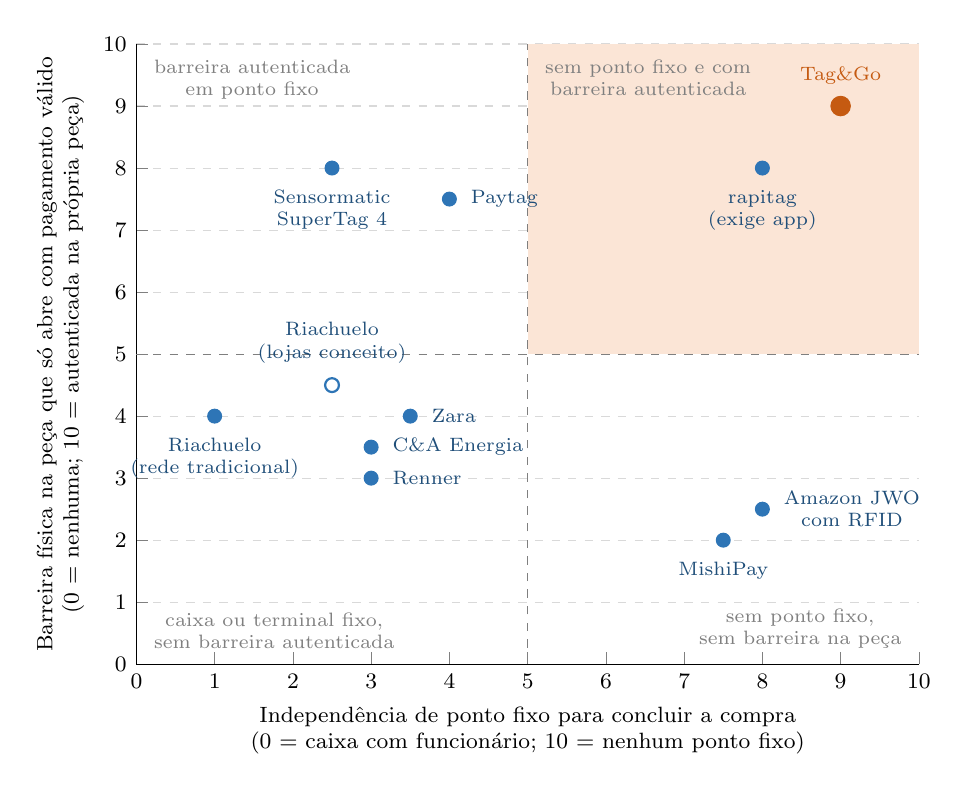
\begin{tikzpicture}
        \begin{axis}[
            r2eixo,
            width=0.95\textwidth,
            height=0.78\textwidth,
            xmin=0, xmax=10, ymin=0, ymax=10,
            xtick={0,1,2,3,4,5,6,7,8,9,10},
            ytick={0,1,2,3,4,5,6,7,8,9,10},
            xlabel={Independência de ponto fixo para concluir a compra\\(0 = caixa com funcionário; 10 = nenhum ponto fixo)},
            ylabel={Barreira física na peça que só abre com pagamento válido\\(0 = nenhuma; 10 = autenticada na própria peça)},
            xlabel style={align=center},
            ylabel style={align=center},
            clip=false,
        ]
            \fill[r2laranjaclaro] (axis cs:5,5) rectangle (axis cs:10,10);
            \draw[dashed, r2cinza] (axis cs:5,0) -- (axis cs:5,10);
            \draw[dashed, r2cinza] (axis cs:0,5) -- (axis cs:10,5);
            \node[r2rotulo, anchor=north west] at (axis cs:5.1,9.9) {sem ponto fixo e com\\barreira autenticada};
            \node[r2rotulo, anchor=north west] at (axis cs:0.1,9.9) {barreira autenticada\\em ponto fixo};
            \node[r2rotulo, anchor=south west] at (axis cs:0.1,0.1) {caixa ou terminal fixo,\\sem barreira autenticada};
            \node[r2rotulo, anchor=south east] at (axis cs:9.9,0.1) {sem ponto fixo,\\sem barreira na peça};
            \addplot[only marks, mark=*, mark size=2.5pt, color=r2azulmedio]
                coordinates {(1,4) (3,3) (3,3.5) (3.5,4) (2.5,8) (4,7.5) (7.5,2) (8,2.5) (8,8)};
            \addplot[only marks, mark=o, mark size=2.5pt, thick, color=r2azulmedio]
                coordinates {(2.5,4.5)};
            \addplot[only marks, mark=*, mark size=3.5pt, color=r2laranja]
                coordinates {(9,9)};
            \node[font=\scriptsize, align=center, text=r2azul, anchor=north] at (axis cs:1,3.8) {Riachuelo\\(rede tradicional)};
            \node[font=\scriptsize, align=center, text=r2azul, anchor=south] at (axis cs:2.5,4.7) {Riachuelo\\(lojas conceito)};
            \node[font=\scriptsize, align=center, text=r2azul, anchor=west] at (axis cs:3.15,3) {Renner};
            \node[font=\scriptsize, align=center, text=r2azul, anchor=west] at (axis cs:3.15,3.5) {C\&A Energia};
            \node[font=\scriptsize, align=center, text=r2azul, anchor=west] at (axis cs:3.65,4) {Zara};
            \node[font=\scriptsize, align=center, text=r2azul, anchor=north] at (axis cs:2.5,7.8) {Sensormatic\\SuperTag 4};
            \node[font=\scriptsize, align=center, text=r2azul, anchor=west] at (axis cs:4.15,7.5) {Paytag};
            \node[font=\scriptsize, align=center, text=r2azul, anchor=north] at (axis cs:7.5,1.8) {MishiPay};
            \node[font=\scriptsize, align=center, text=r2azul, anchor=west] at (axis cs:8.15,2.5) {Amazon JWO\\com RFID};
            \node[font=\scriptsize, align=center, text=r2azul, anchor=north] at (axis cs:8,7.8) {rapitag\\(exige app)};
            \node[font=\scriptsize, align=center, text=r2laranja, anchor=south] at (axis cs:9,9.2) {Tag\&Go};
        \end{axis}
    \end{tikzpicture}
    \source{Elaborado pelos autores (2026), com posições estimadas pela equipe a partir das fontes da Tabela~\ref{tab:r2-diferenciacao}. Marcador vazado: tecnologia da etiqueta não divulgada.}
\end{figure}

O quadrante superior direito, que reúne liberação sem ponto fixo e barreira autenticada, tem apenas duas soluções: a rapitag, que exige o app do varejista, e o Tag\&Go. O quadrante inferior esquerdo concentra o varejo de moda brasileiro, inclusive a Renner, líder no benchmarking do Relatório 1, e daí a equipe concluiu que o self-checkout em terminal fixo virou prática do segmento e já não distingue quem o adota. As lojas conceito da Riachuelo aparecem com marcador vazado porque sua posição vertical é incerta: se a etiqueta inteligente tiver barreira autenticada, o ponto sobe em direção à SuperTag 4, mas continua à esquerda, preso ao terminal. A distância entre o Tag\&Go e a rede tradicional da Riachuelo, nos dois eixos, mede o salto que o sistema propõe à empresa.

\subsection{Diferenciais do Tag\&Go}
\label{sub:r2-dif-diferenciais}

A partir da tabela e do mapa, a equipe identificou cinco diferenciais, codificados de DF1 a DF5 para não se confundirem com os desejos D01 a D07 do Relatório 1. Cada diferencial foi definido pelo contraste com uma referência concreta, e não pela descrição do próprio produto.

O primeiro diferencial (DF1) é o pagamento em qualquer ponto da loja com liberação na própria peça, sem terminal fixo no fluxo principal. Frente às lojas conceito da Riachuelo, à Renner e à C\&A, o Tag\&Go elimina o ponto de pagamento; frente à Paytag e à SuperTag 4, elimina a estação de remoção. O único ponto fixo que resta é o Liberador de Balcão, usado nas exceções, como celular sem bateria ou etiqueta sem energia, e é ele que garante a alternativa humana exigida por R07.

O segundo diferencial (DF2) é a autorização verificada na própria etiqueta. A etiqueta gera um desafio a cada liberação, um nonce, e só aceita um token calculado para aquele desafio, aquela etiqueta e aquela transação; o celular apenas retransmite o token e não guarda segredo, de modo que um aparelho adulterado não consegue forjá-lo. Com o carretel não ferromagnético, a etiqueta também fica imune ao destacador magnético comum, vendido livremente por cerca de R\$~300 \cite{canalautomacao2026desacoplador}, que abre tanto a etiqueta da rede tradicional quanto qualquer etiqueta rígida comercial. O protocolo completo está na Seção~\ref{sec:r2-arquitetura}. Frente à rapitag, única outra referência com barreira na peça, a equipe não comparou o esquema de autorização, porque não o verificou; o DF2 foi afirmado, portanto, frente às demais referências.

O terceiro diferencial (DF3) é a Compra Rápida sem instalar aplicativo nas duas plataformas, pelo App Clip Tag\&Go no iPhone e pela Página de Compra Rápida no Android, combinada com a barreira física na peça. Nas duas plataformas, o cliente paga pela carteira do celular, com Apple Pay ou Google Pay e confirmação por Face ID, Touch ID ou senha na folha do sistema, ou por Pix copia e cola, sem cadastro prévio. A rapitag, a Paytag e a C\&A exigem app, e a Zara exige o app para o Store Mode. O web app da MishiPay na Flying Tiger é o precedente mais próximo de compra sem app \cite{mishipay2026flyingtiger}, só que sem etiqueta rígida. O diferencial tem duas dependências que a equipe declara desde já: no iPhone, o uso de Core Bluetooth dentro do App Clip foi deduzido da documentação da Apple, que não o proíbe, e será o primeiro teste de go/no-go do protótipo \cite{apple2026appclipfuncoes}; e o App Clip exige que o app Riachuelo publique a mesma função \cite{apple2026appclipcriar}. No Android, a página depende do Web Bluetooth, disponível no Chrome para Android e no Samsung Internet \cite{chrome2026webbluetooth}.

O quarto diferencial (DF4) é o ciclo fechado de uma etiqueta ativa, com cadastro na origem, no ramo fábrica (peças próprias, em Natal) ou no ramo CD (peças de terceiros), e recarga no CD, de modo que a loja não etiqueta nem cadastra peças. A recirculação de etiquetas passivas já existe: a Sensormatic recolhe etiquetas e pinos no ponto de venda e os devolve às fábricas \cite{sensormatic2024recirculacao}, a Pact relata reuso de até 80\% \cite{pact2026etiquetas}, e a Inditex recircula as suas com a Tyco \cite{rfidjournal2014inditex}. O que muda no Tag\&Go é fazer isso com uma etiqueta que tem bateria e chave criptográfica, o que acrescenta ao ciclo a inspeção, a recarga e a associação da etiqueta ao EPC da peça, descritas na Subseção~\ref{sub:r2-ciclo}. O trabalho de aplicar a etiqueta não desaparece; ele sai da loja e passa à origem. A meta de retorno de 99\% por ciclo (S01) fica acima dos 80\% a 83\% observados no mercado (Subseção~\ref{sub:r2-especificacoes}) e é tratada como meta, com os mecanismos e as consequências econômicas discutidos na Seção~\ref{sec:r2-valor}.

O quinto diferencial (DF5) é a Jornada Completa ligada ao Ria Club, no módulo Tag\&Go do app Riachuelo: um perfil com tamanhos e preferências, recomendação só do que existe na loja no tamanho do perfil, compra on-line do tamanho ausente, com retirada na loja sem custo ou entrega sem frete acima de um valor mínimo a definir com a Riachuelo, e métricas de sustentabilidade apresentadas como estimativa por categoria, com o cashback liberado depois que a etiqueta é devolvida ao Coletor de Etiquetas. Como o app Riachuelo não localiza a peça na loja nem mostra o estoque por loja, a Jornada Completa aproveita a base RFID que a rede já tem para preencher essa lacuna. A localização da peça entra como função secundária, no nível N1, o setor, obtido do estoque RFID e de um planograma digital, sem depender da etiqueta (Subseção~\ref{sub:r2-localizar}). Trata-se de um diferencial de experiência e de dados, sem relação com o hardware, e apoiado em hipóteses: o survey do Relatório 1 não mediu interesse por fidelidade, recomendação ou sustentabilidade.

A equipe também registrou o que não é diferencial, para não vender como novidade o que o mercado já oferece. O self-checkout em si já existe na Renner, na C\&A e nas lojas conceito da Riachuelo; o RFID, segundo a própria empresa, já está em todos os produtos da Riachuelo \cite{neofeed2025riachuelo}; o pagamento por carteira digital é oferecido pela MishiPay e por qualquer loja que aceite Apple Pay ou Google Pay; a localização da peça na planta da loja é feita pela Zara \cite{inditex2021storemode}; e o cashback já está no Ria Club e no C\&A Pay \cite{midway2026riaclub,cea2026pay}. Esses elementos entram no Tag\&Go como parte do núcleo comum ou da Jornada Completa, e a diferenciação vem da forma como o sistema os combina com a liberação na peça.

\subsection{Riscos de diferenciação}
\label{sub:r2-dif-riscos}

A posição do Tag\&Go no mapa pode ser contestada por três caminhos. O primeiro é a entrada no Brasil das duas empresas mais próximas. A Paytag já tem uso comercial em Israel e afirma ter patente registrada globalmente \cite{calcalist2026paytag}, e a rapitag já fez um piloto com um varejista na Alemanha e divide com o Tag\&Go o quadrante superior direito do mapa. Contra a rapitag, o DF3 é o diferencial mais defensável, porque a compra sem app depende de recursos de plataforma que a equipe já mapeou; contra a Paytag, pesa o DF1. O segundo caminho é a própria Riachuelo: como a tecnologia das lojas conceito não foi divulgada, ela pode já cobrir parte do DF1, e a equipe precisa confirmar com a empresa o que a etiqueta inteligente faz antes de apresentar o Tag\&Go como substituto. O terceiro caminho é a propriedade intelectual, já que há patentes de etiquetas que se destacam depois de uma compra verificada no celular; a análise das famílias de patentes está na Seção~\ref{sec:r2-aproveitamento}, e a busca no INPI ficou para o Relatório 3.

Os diferenciais também têm durabilidades diferentes. O DF5 é o mais fácil de copiar, porque depende de software e de dados que qualquer varejista com app e RFID pode reunir, como já faz a Renner. O DF2 e o DF4 são os mais difíceis, porque exigem ao mesmo tempo a etiqueta ativa, o protocolo de autorização e a logística reversa com cadastro na origem. O DF1 e o DF3 ficam no meio: são visíveis para o cliente, e por isso mais fáceis de imitar, mas só funcionam com a barreira na peça; o DF3 depende ainda de a Riachuelo manter no app a função equivalente ao App Clip.

Por fim, a equipe ligou os diferenciais às notas do Relatório 1. Na casa da qualidade, a Riachuelo recebeu nota 2 na redução da espera no caixa (DE01) e no pagamento rápido sem perder o atendimento (DE05), as duas vozes que somaram 50,5\% do peso relativo. O DF1 e o DF3 atacam DE01, ao retirar o caixa e o terminal do fluxo principal; o Liberador de Balcão e o Ponto de Apoio preservam o atendimento pedido em DE05. Com esses diferenciais, o Tag\&Go mira nota 5 nas duas vozes, o que em DE05 fica acima do plano de qualidade de 4 fixado no Relatório 1. As metas quantitativas correspondentes, de tempo de pagamento, compra sem funcionário e clareza do fluxo, estão nas especificações-meta da Tabela~\ref{tab:r2-especificacoes} e serão verificadas no protótipo.

\newpage% =============================================================================
% Relatorio 2, Secao 4: escala vertical e valor mercadologico (item C).
% Conteudo: metodo; escala vertical (TAB08, FIG06); custo da etiqueta e
% custo-meta (TAB09); frota em uma linha, custo por uso e taxa de retorno
% (FIG07); valor economico para a Riachuelo (TAB10, FIG08); preco e
% remuneracao do fornecedor; sensibilidade do equilibrio (FIG09).
% Todos os numeros saem do script canonico conta_final.py (biblia, parte 2.11).
% A composicao da frota fica na Secao 7 (sub:r2-ciclo e fig:r2-frota).
% =============================================================================

\section{ESCALA VERTICAL E VALOR MERCADOLÓGICO}
\label{sec:r2-valor}

Os diferenciais identificados na Seção~\ref{sec:r2-diferenciacao} só têm valor comercial se o varejista puder pagar por eles. O item C do projeto conceitual trata dessa questão ao pedir a escala vertical de preços e a definição do valor mercadológico do produto \cite{zancul2026conceitual}. No Tag\&Go, essa definição tem uma particularidade: quem compra o sistema é o varejista, e o consumidor usa a etiqueta sem pagar nada a mais. Por isso, a equipe tratou o valor como uma questão de viabilidade econômica para dois agentes, a Riachuelo, que precisa recuperar o que paga pelo sistema, e o fornecedor, que precisa remunerar o capital imobilizado na frota de etiquetas. Acompanhar a viabilidade econômica também é uma das atividades que \citeonline{rozenfeld2006gestao} atribuem à fase conceitual.

\subsection{Método}
\label{sub:r2-valor-metodo}

O Tag\&Go é vendido a um varejista (B2B) e não tem concorrente direto à venda no Brasil, o que impede comparar o seu preço com o de um produto equivalente. A equipe seguiu, então, o precedente do projeto USPontos de Recarga, relatório de anos anteriores da disciplina consultado pela equipe, que também tratava de um produto vendido a uma instituição: a escala vertical foi montada com produtos que cumprem parte das funções do Tag\&Go ou que o varejista já compra, e o valor foi definido pelo valor econômico para o comprador, com análise de equilíbrio e de retorno do investimento. A escala serve para posicionar o produto entre referências que o comprador conhece e não justifica o preço, que decorre da conta econômica das Subseções~\ref{sub:r2-valor-riachuelo} e \ref{sub:r2-preco}.

Os precedentes PenDrive e HotPot, também de anos anteriores, posicionaram o produto na escala com pesquisa de clientes. Neste projeto não houve pesquisa com o comprador B2B, e os preços de equipamentos, os parâmetros da loja e as premissas de operação usados adiante foram estimados pela equipe a partir de fontes públicas. Essa é uma limitação do estudo, que a validação com a Riachuelo e o piloto deverão reduzir. Os valores em dólar foram convertidos pela PTAX de venda do Banco Central de 25/09/2026, R\$~5,1991 por US\$ \cite{bcb2026ptax}, e todas as contas econômicas saíram de um único script de cálculo da equipe, de modo que texto, tabelas e figuras usam os mesmos números.

\subsection{Escala vertical de preços}
\label{sub:r2-escala}

A escala reúne 25 itens, 23 produtos de referência em cinco categorias e dois valores do Tag\&Go, ordenados do mais barato ao mais caro na Tabela~\ref{tab:r2-escala}. Os consumíveis EAS são o que a Riachuelo já compra para proteger as peças e o que a etiqueta Tag\&Go substitui. Os componentes de identificação (inlay RFID e adesivo NFC) mostram o custo de identificar uma peça sem nenhuma função ativa. As etiquetas eletrônicas de prateleira (ESL) são a referência mais próxima em arquitetura, porque também têm rádio e bateria. Os rastreadores BLE de consumo são o produto de massa mais próximo em eletrônica, e os itens de infraestrutura, dos desacopladores magnéticos aos terminais de self-checkout, representam o que o varejista compra para operar a prevenção de perdas e o autoatendimento. O Tag\&Go entra com dois valores, o custo-meta de fabricação (Subseção~\ref{sub:r2-custo-meta}) e o preço de venda na modalidade compra (Subseção~\ref{sub:r2-preco}).

\begin{table}[htbp]
    \centering
    \caption{Escala vertical de preços}
    \label{tab:r2-escala}
    \scriptsize
    \setlength{\tabcolsep}{4pt}
    \renewcommand{\arraystretch}{1.25}
    \begin{tabularx}{\textwidth}{@{}
        >{\raggedleft\arraybackslash}p{0.5cm}
        >{\RaggedRight\arraybackslash}X
        >{\raggedleft\arraybackslash}p{1.5cm}
        >{\RaggedRight\arraybackslash}p{2.5cm}
        >{\RaggedRight\arraybackslash}p{3.9cm}@{}}
        \toprule
        \textbf{Nº} & \textbf{Item} & \textbf{R\$} & \textbf{Categoria} & \textbf{Fonte} \\
        \midrule
        1 & Pino para etiqueta rígida (lote de 1.000) & 0,12 & Consumível EAS & \citeonline{canalautomacao2026pino} \\
        2 & Etiqueta adesiva RF 8,2\,MHz (rolo de 1.000) & 0,18 & Consumível EAS & \citeonline{sensormagic2026adesiva} \\
        3 & Etiqueta rígida RF 8,2\,MHz, importação (US\$~0,05) & 0,26 & Consumível EAS & \citeonline{alibaba2026rf} \\
        4 & Etiqueta rígida AM pencil (caixa de 1.000) & 0,30 & Consumível EAS & \citeonline{hexport2026pencil} \\
        5 & Inlay RFID UHF de vestuário (US\$~0,12) & 0,62 & Identificação & \citeonline{atlasrfid2026tags} \\
        6 & Etiqueta rígida mini tag RF com pino (lote de 2.000) & 0,87 & Consumível EAS & \citeonline{allcard2026minitag} \\
        7 & Etiqueta rígida AM pencil, varejo (milheiro) & 1,32 & Consumível EAS & \citeonline{canalautomacao2026pencil} \\
        8 & Adesivo NFC NTAG213 & 2,03 & Identificação & \citeonline{smartkits2026ntag} \\
        9 & ESL, faixa baixa (US\$~5) & 26,00 & Eletrônico de prateleira & \citeonline{solum2026esl} \\
        10 & ESL, faixa alta (US\$~10) & 51,99 & Eletrônico de prateleira & \citeonline{solum2026esl} \\
        \rowcolor{r2laranjaclaro}
        11 & Tag\&Go, custo-meta & 60,00 & Tag\&Go & Tabela~\ref{tab:r2-bom} \\
        \rowcolor{r2laranjaclaro}
        12 & Tag\&Go, preço de venda na modalidade compra & 90,00 & Tag\&Go & Subseção~\ref{sub:r2-preco} \\
        13 & Tile, preço de lista (US\$~24,99) & 129,93 & Rastreador & \citeonline{nbc2026tile} \\
        14 & Desacoplador 5.200\,GS & 168,90 & Infraestrutura & \citeonline{drich2026desacoplador} \\
        15 & Desacoplador 10.000\,GS & 300,00 & Infraestrutura & \citeonline{canalautomacao2026desacoplador} \\
        16 & Galaxy SmartTag2 (lançamento) & 349,00 & Rastreador & \citeonline{olhardigital2023smarttag} \\
        17 & Desacoplador 11.500\,GS & 359,00 & Infraestrutura & \citeonline{allcard2026desacoplador} \\
        18 & AirTag de 2ª geração & 369,00 & Rastreador & \citeonline{apple2026airtag} \\
        19 & Quiosque Elgin MK 11 & 4.162,00 & Infraestrutura & \citeonline{elgin2026selfcheckout} \\
        20 & Antena EAS AM TX/RX & 5.099,00 & Infraestrutura & \citeonline{i9automacao2026antena} \\
        21 & Leitor RFID Zebra FXP20 (US\$~984,50) & 5.118,51 & Infraestrutura & \citeonline{atlasrfid2026leitor} \\
        22 & Self-checkout de varejo, piso (US\$~2.000) & 10.398,20 & Infraestrutura & \citeonline{korona2026selfcheckout} \\
        23 & Quiosque Elgin MK 21 & 13.008,00 & Infraestrutura & \citeonline{elgin2026selfcheckout} \\
        24 & Self-checkout de varejo, teto (US\$~15.000) & 77.986,50 & Infraestrutura & \citeonline{korona2026selfcheckout} \\
        25 & Self-checkout com RFID ou visão (acima de US\$~20.000) & 103.982,00 & Infraestrutura & \citeonline{korona2026selfcheckout} \\
        \bottomrule
    \end{tabularx}
    \source{Elaborado pelos autores (2026) com base nas fontes indicadas na tabela; valores em dólar convertidos pela PTAX de venda de 25/09/2026 \cite{bcb2026ptax}.}
\end{table}

Como os preços cobrem seis ordens de grandeza, de R\$~0,12 a R\$~103.982,00, a Figura~\ref{fig:r2-escala-vertical} representa a escala com eixo logarítmico e cores por categoria.

\begin{figure}[htbp]
    \centering
    \caption{Escala vertical de preços}
    \label{fig:r2-escala-vertical}
    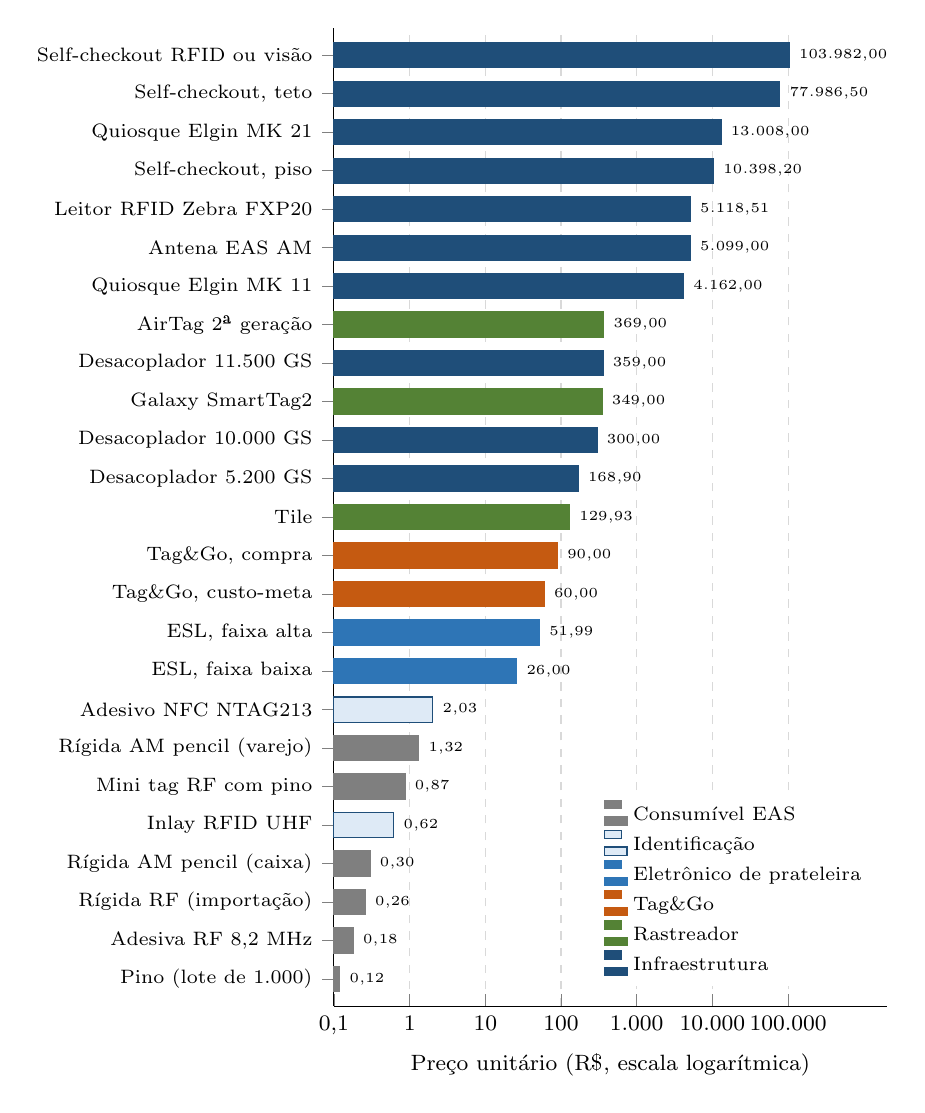
\begin{tikzpicture}
        \begin{axis}[
            r2eixo,
            xbar, bar shift=0pt, bar width=3.2mm,
            xmode=log, log basis x=10, log origin x=infty,
            xmin=0.1, xmax=2000000,
            ymin=0.3, ymax=25.7,
            width=8.6cm, height=14cm,
            ymajorgrids=false, xmajorgrids,
            ytick={1,2,...,25},
            yticklabels={
                {Pino (lote de 1.000)},
                {Adesiva RF 8,2 MHz},
                {Rígida RF (importação)},
                {Rígida AM pencil (caixa)},
                {Inlay RFID UHF},
                {Mini tag RF com pino},
                {Rígida AM pencil (varejo)},
                {Adesivo NFC NTAG213},
                {ESL, faixa baixa},
                {ESL, faixa alta},
                {Tag\&Go, custo-meta},
                {Tag\&Go, compra},
                {Tile},
                {Desacoplador 5.200 GS},
                {Desacoplador 10.000 GS},
                {Galaxy SmartTag2},
                {Desacoplador 11.500 GS},
                {AirTag 2ª geração},
                {Quiosque Elgin MK 11},
                {Antena EAS AM},
                {Leitor RFID Zebra FXP20},
                {Self-checkout, piso},
                {Quiosque Elgin MK 21},
                {Self-checkout, teto},
                {Self-checkout RFID ou visão}},
            y tick label style={font=\scriptsize},
            xtick={0.1,1,10,100,1000,10000,100000},
            xticklabels={{0,1},1,10,100,{1.000},{10.000},{100.000}},
            xlabel={Preço unitário (R\$, escala logarítmica)},
            point meta=rawx,
            nodes near coords={\pgfmathprintnumber[fixed,fixed zerofill,precision=2,use comma,1000 sep={.}]{\pgfplotspointmeta}},
            nodes near coords align={horizontal},
            every node near coord/.append style={font=\tiny, text=black},
            legend style={at={(0.98,0.02)}, anchor=south east, font=\scriptsize, draw=none, fill=white},
            legend cell align=left,
            clip=false,
        ]
            \addplot[fill=r2cinza, draw=r2cinza] coordinates {(0.12,1) (0.18,2) (0.26,3) (0.30,4) (0.87,6) (1.32,7)};
            \addlegendentry{Consumível EAS}
            \addplot[fill=r2azulclaro, draw=r2azul] coordinates {(0.62,5) (2.03,8)};
            \addlegendentry{Identificação}
            \addplot[fill=r2azulmedio, draw=r2azulmedio] coordinates {(26.00,9) (51.99,10)};
            \addlegendentry{Eletrônico de prateleira}
            \addplot[fill=r2laranja, draw=r2laranja] coordinates {(60.00,11) (90.00,12)};
            \addlegendentry{Tag\&Go}
            \addplot[fill=r2verde, draw=r2verde] coordinates {(129.93,13) (349.00,16) (369.00,18)};
            \addlegendentry{Rastreador}
            \addplot[fill=r2azul, draw=r2azul] coordinates {(168.90,14) (300.00,15) (359.00,17) (4162.00,19) (5099.00,20) (5118.51,21) (10398.20,22) (13008.00,23) (77986.50,24) (103982.00,25)};
            \addlegendentry{Infraestrutura}
        \end{axis}
    \end{tikzpicture}
    \source{Elaborado pelos autores (2026) com base nas fontes da Tabela~\ref{tab:r2-escala}.}
\end{figure}

A equipe fez três leituras da escala. A primeira é de coerência técnica: o custo-meta do Tag\&Go, R\$~60, fica entre a ESL (R\$~26,00 a R\$~51,99), que também tem rádio e bateria, e os rastreadores BLE de consumo (R\$~129,93 a R\$~369,00), posição compatível com um dispositivo BLE que ainda tem atuador e trava mecânica. A segunda é de ordem de grandeza frente ao que o produto substitui: a mini tag RF com pino custa R\$~0,87, e a etiqueta Tag\&Go custa cerca de 70 vezes mais. Uma diferença desse tamanho só se viabiliza se a etiqueta for tratada como ativo reutilizável, cobrado por uso, o que orientou o modelo de locação da Subseção~\ref{sub:r2-preco}. A terceira situa o investimento do varejista: o sistema de uma loja é comparado com itens de infraestrutura que o varejista já compra, como antenas EAS, leitores RFID e terminais de self-checkout, cujos preços unitários vão de R\$~4.162,00 a R\$~103.982,00. No Brasil, o self-checkout é vendido por compra, locação, leasing, Finame e cartão BNDES, sem preço publicado \cite{perto2021selfcheckout}, o que mostra que o comprador já conhece a contratação de equipamentos de loja por locação.

A escala tem ressalvas. Os preços do varejo brasileiro de automação vieram de páginas e títulos de anúncio, com confiança média, e podem ter mudado; os preços em dólar são de distribuidor, sem impostos de importação; o Galaxy SmartTag2 aparece com o preço de lançamento de 2023; e o Tile aparece com o preço de lista, embora a página consultada traga uma oferta. Nenhuma dessas ressalvas altera a posição relativa do Tag\&Go, que depende de diferenças de uma ordem de grandeza ou mais.

\subsection{Custo da etiqueta e custo-meta}
\label{sub:r2-custo-meta}

A equipe estimou o custo da etiqueta em três colunas, reunidas na Tabela~\ref{tab:r2-bom}: o protótipo, com os componentes de varejo que serão comprados para o Relatório 3; a produção em escala sem redesenho, isto é, a etiqueta do Relatório 1 fabricada com preços de volume; e a meta de \textit{design to cost}, que incorpora as mudanças de projeto adotadas no Relatório 2. Os grupos da tabela seguem os componentes da etiqueta descritos na Seção~\ref{sec:r2-arquitetura}.

\begin{table}[htbp]
    \centering
    \caption{Custo da etiqueta Tag\&Go e custo-meta}
    \label{tab:r2-bom}
    \scriptsize
    \setlength{\tabcolsep}{4pt}
    \renewcommand{\arraystretch}{1.25}
    \begin{tabularx}{\textwidth}{@{}
        >{\RaggedRight\arraybackslash}p{2.3cm}
        >{\raggedleft\arraybackslash}p{1.35cm}
        >{\raggedleft\arraybackslash}p{1.6cm}
        >{\raggedleft\arraybackslash}p{1.6cm}
        >{\RaggedRight\arraybackslash}X@{}}
        \toprule
        \textbf{Grupo} & \textbf{Protótipo (R\$)} & \textbf{Escala sem redesenho (R\$)} & \textbf{Meta de \textit{design to cost} (R\$)} & \textbf{Origem da redução} \\
        \midrule
        Controle e rádio & 25,00 & 10,45 & 10,45 & ESP32-C3 Super Mini no protótipo; em escala, módulo ESP32-C3-MINI-1 com certificado Anatel (US\$~2,01); mantido na meta \\
        Energia & 31,00 & 33,75 & 9,50 & LiPo de 300\,mAh e módulo TP4056 $\rightarrow$ célula de 150\,mAh com proteção, suficiente para autonomia $\geq 2T$ no modo botão (E05), e CI de carga na placa única; preço de volume da célula a cotar \\
        Atuação & 36,40 & 32,30 & 9,20 & protótipo com micromotor N20 (R\$~28,00); escala sem redesenho com o servo MG90S do Relatório 1; meta com micromotor com redução e came e driver na placa (clone de cerca de US\$~1,66, preço de anúncio, baixa confiança) \\
        Interface & 7,00 & 6,44 & 2,60 & LED RGB, chave e buzzer em módulos $\rightarrow$ componentes SMD e piezo na placa \\
        Identificação & 4,03 & 3,03 & 1,80 & NTAG213 e manta de ferrite sob o QR (ferrite estimado) \\
        Retenção e EAS & 1,70 & 0,87 & 0,87 & garra, pino e elemento EAS de mini tag comercial \\
        Carcaça e fixação & 13,70 & 18,48 & 18,48 & PETG impresso $\rightarrow$ duas peças injetadas (US\$~1,70 cada, exemplo hipotético) e parafusos de segurança \\
        Contatos de serviço & 2,00 & 0,60 & 0,60 & três pads rebaixados na face superior \\
        Placa e montagem & 3,00 & 5,00 & 4,00 & fiação no protótipo $\rightarrow$ placa única montada em SMT \\
        \midrule
        Subtotal & 123,83 & 110,91 & 57,50 & \\
        Reserva de montagem (10\%) & 12,38 & 11,09 & 5,75 & 10\% do subtotal, sem ajuste \\
        \midrule
        Total & 136,21 & 122,00 & 63,25 & meta de R\$~60 $\pm$ 10\% (R\$~54 a R\$~66) \\
        \bottomrule
    \end{tabularx}
    \source{Elaborado pelos autores (2026) com base em \citeonline{digikey2026esp32}, \citeonline{adafruit2026lipo}, \citeonline{curtocircuito2026n20}, \citeonline{pololu2026n20}, \citeonline{formlabs2026injecao}, \citeonline{lcsc2026chave}, \citeonline{digikey2026led}, \citeonline{smartkits2026ntag}, \citeonline{allcard2026minitag} e estudos anteriores da equipe.}
\end{table}

O custo-meta foi fixado em R\$~60 $\pm$ 10\%, isto é, entre R\$~54 e R\$~66, faixa que a composição da meta, R\$~63,25, atende. A redução de 48,2\% em relação à escala sem redesenho (R\$~122,00) vem de três decisões de projeto, cada uma com justificativa técnica própria, e não de um ajuste feito para fechar a conta. A primeira é trocar a LiPo de 300\,mAh por uma célula de 150\,mAh com proteção: com a etiqueta no modo botão, que só acorda quando o cliente aperta o botão, a autonomia estimada pela equipe é de 448 dias, contra a meta de 168 dias da especificação E05 (Tabela~\ref{tab:r2-especificacoes}), e a célula maior deixou de ser necessária. A segunda é substituir o servo MG90S do Relatório 1 por um micromotor com redução, que aciona o mesmo cursor com rampa por meio de um came e ocupa menos altura. A terceira é reunir módulo de rádio, CI de carga, driver do motor, LED e buzzer em uma placa única montada em SMT, o que elimina os módulos avulsos do protótipo e reduz a montagem manual.

Dois grupos não mudam entre a escala sem redesenho e a meta. O módulo ESP32-C3-MINI-1, a US\$~2,01 em rolo \cite{digikey2026esp32}, foi mantido porque tem certificado Anatel \cite{espressif2026certificados}, o que simplifica a homologação do produto final. A carcaça injetada, a US\$~1,70 por peça, foi estimada a partir de um exemplo hipotético de gabinete eletrônico com molde de aço de US\$~20 mil e 100 mil unidades, que não é um orçamento \cite{formlabs2026injecao}. Três preços da meta ainda precisam de cotação, que é um dos próximos passos do Relatório 3: o da célula, porque o único preço de volume encontrado para uma célula pequena, US\$~4,76 (R\$~24,75) por uma LiPo de 100\,mAh com proteção, vale para lotes de 100 unidades \cite{adafruit2026lipo}, volume muito inferior ao de uma frota; o do micromotor, cuja referência de meta é um preço de anúncio de baixa confiança, enquanto um micromotor de marca com redução de 298:1 custa US\$~18,65 em lotes de 100 \cite{pololu2026n20}; e o do molde. Para o protótipo, a lista de compras do Relatório 3 soma R\$~606,65 para duas etiquetas com came por micromotor, buzzer, NFC e ferrite, ou R\$~101,11 por aluno.

\subsection{Frota, custo por uso e taxa de retorno}
\label{sub:r2-custo-uso}

As contas econômicas partem de uma loja padrão, estimada pela equipe a partir de fontes públicas. A fábrica de Natal produziu cerca de 37 milhões de peças em 2025, o que corresponde a cerca de 40\% do que a rede vende \cite{bloomberglinea2026riachuelo}; a rede vendeu, portanto, cerca de 92,5 milhões de peças, e a receita de vestuário de R\$~6,5 bilhões \cite{abvtex2026riachuelo} dá um preço médio de R\$~70,27 por peça. Dividindo as vendas físicas (descontada a penetração digital de 8\% registrada em 2024 \cite{btg2025guararapes}) pelas 342 lojas Riachuelo \cite{abvtex2026riachuelo}, a loja padrão vende $V = 682$ peças por dia. A equipe adotou como premissa que $f = 10\%$ dessas peças recebem etiqueta rígida, o que dá $S = 68$ liberações por dia e $L = 24.820$ liberações por ano por loja, e que cada compra tem 3 peças, o que dá 227 compras por dia.

A frota por loja, também uma premissa de trabalho, foi dimensionada pela lei de Little:
\begin{equation}
N = S \times T \times k = 68 \times 84 \times 1{,}2 \approx 6.854 \text{ etiquetas por loja},
\end{equation}
em que $T = 84$ dias é o ciclo médio da etiqueta, que inclui a permanência em loja de 60 dias, premissa ancorada no prazo médio de estoques de 95 dias da Renner \cite{renner2026resultados}, e $k = 1{,}2$ é a reserva para variabilidade e perdas no processo. A composição da frota por etapa do ciclo está na Subseção~\ref{sub:r2-ciclo} e na Figura~\ref{fig:r2-frota}.

Como o ciclo é longo, a etiqueta circula pouco. Com $365/(T \times k) = 3{,}62$ ciclos por ano e vida de 5 anos (premissa), cada etiqueta faz no máximo $U = 18{,}1$ ciclos. Se a etiqueta volta ao CD com probabilidade $r$ a cada ciclo, o número esperado de usos $E(r)$ e o custo por uso de uma etiqueta de custo $C$ são:
\begin{equation}
E(r) = \frac{1 - r^{U}}{1 - r}, \qquad \text{custo por uso} = \frac{C}{E(r)}.
\end{equation}

A Figura~\ref{fig:r2-custo-uso} mostra o custo por uso para o custo-meta (R\$~60) e para a escala sem redesenho (R\$~122), em função da taxa de retorno.

\begin{figure}[htbp]
    \centering
    \caption{Custo por uso da etiqueta em função da taxa de retorno}
    \label{fig:r2-custo-uso}
    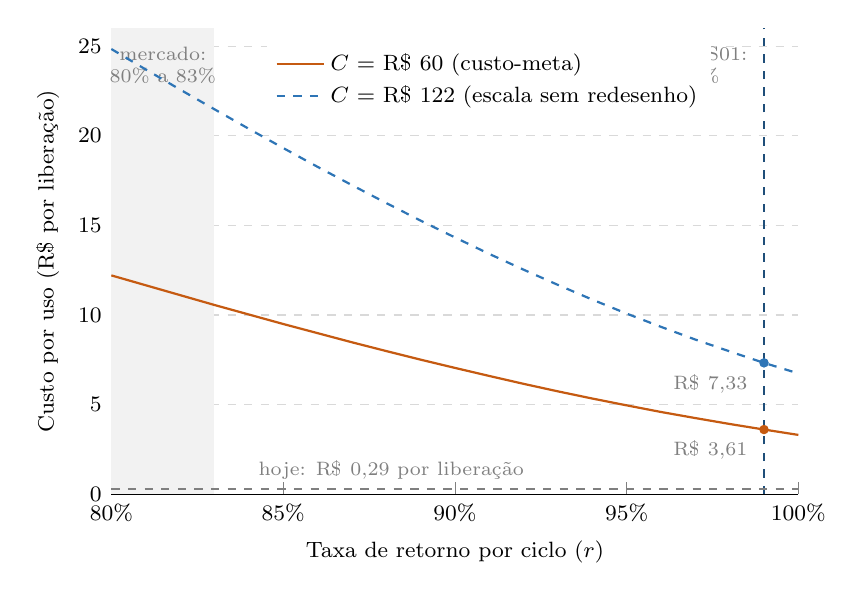
\begin{tikzpicture}
        \begin{axis}[
            r2eixo,
            width=0.85\textwidth, height=7.5cm,
            xmin=0.80, xmax=1.00, ymin=0, ymax=26,
            xtick={0.80,0.85,0.90,0.95,1.00},
            xticklabels={80\%,85\%,90\%,95\%,100\%},
            ytick={0,5,10,15,20,25},
            xlabel={Taxa de retorno por ciclo ($r$)},
            ylabel={Custo por uso (R\$ por liberação)},
            legend style={at={(0.55,0.97)}, anchor=north, font=\footnotesize, draw=none, fill=white},
            legend cell align=left,
            clip=false,
        ]
            \fill[r2cinzaclaro] (axis cs:0.80,0) rectangle (axis cs:0.83,26);
            \node[r2rotulo, anchor=north] at (axis cs:0.815,25.5) {mercado:\\80\% a 83\%};
            \addplot[r2laranja, thick, mark=none] coordinates {
                (0.80,12.21) (0.81,11.66) (0.82,11.11) (0.83,10.56) (0.84,10.03)
                (0.85,9.50) (0.86,8.99) (0.87,8.48) (0.88,7.99) (0.89,7.51)
                (0.90,7.05) (0.91,6.60) (0.92,6.16) (0.93,5.74) (0.94,5.34)
                (0.95,4.96) (0.96,4.59) (0.97,4.25) (0.98,3.92) (0.99,3.61) (1.00,3.31)};
            \addlegendentry{$C$ = R\$~60 (custo-meta)}
            \addplot[r2azulmedio, thick, dashed, mark=none] coordinates {
                (0.80,24.84) (0.81,23.70) (0.82,22.58) (0.83,21.48) (0.84,20.39)
                (0.85,19.32) (0.86,18.27) (0.87,17.25) (0.88,16.25) (0.89,15.27)
                (0.90,14.33) (0.91,13.41) (0.92,12.53) (0.93,11.68) (0.94,10.86)
                (0.95,10.08) (0.96,9.34) (0.97,8.63) (0.98,7.97) (0.99,7.33) (1.00,6.74)};
            \addlegendentry{$C$ = R\$~122 (escala sem redesenho)}
            \draw[r2azul, dashed] (axis cs:0.99,0) -- (axis cs:0.99,26);
            \node[r2rotulo, anchor=north east] at (axis cs:0.988,25.5) {meta S01:\\99\%};
            \addplot[only marks, mark=*, mark size=1.5pt, r2laranja, forget plot] coordinates {(0.99,3.61)};
            \addplot[only marks, mark=*, mark size=1.5pt, r2azulmedio, forget plot] coordinates {(0.99,7.33)};
            \node[r2rotulo, anchor=north east] at (axis cs:0.988,3.5) {R\$~3,61};
            \node[r2rotulo, anchor=north east] at (axis cs:0.988,7.2) {R\$~7,33};
            \draw[r2cinza, dashed] (axis cs:0.80,0.29) -- (axis cs:1.00,0.29);
            \node[r2rotulo, anchor=south west] at (axis cs:0.84,0.29) {hoje: R\$~0,29 por liberação};
        \end{axis}
    \end{tikzpicture}
    \source{Elaborado pelos autores (2026) com base em \citeonline{pact2026etiquetas} e \citeonline{sensormatic2024recirculacao}.}
\end{figure}

A curva deixa clara a dependência da economia em relação ao retorno. Com o custo-meta, o custo por uso cai de R\$~12,21 a 80\% de retorno para R\$~10,56 a 83\%, R\$~7,05 a 90\%, R\$~4,96 a 95\% e R\$~3,61 a 99\%, quando a etiqueta faz em média 16,64 usos; mesmo com retorno total, o custo não desce de R\$~3,31. Com o custo da escala sem redesenho, os valores dobram: R\$~21,48 a 83\% e R\$~7,33 a 99\%. Em todos os casos, o custo por uso fica acima dos R\$~0,29 que a Riachuelo gasta hoje por liberação com a etiqueta rígida comum (Subseção~\ref{sub:r2-valor-riachuelo}). Como a proteção fica mais cara, a vantagem do Tag\&Go precisa vir do que a liberação pelo celular devolve em vendas e em tempo de caixa. A experiência dos \textit{pools} de ativos retornáveis confirma o peso do retorno nessa conta: na Brambles, que opera paletes em \textit{pool}, a queda das perdas não compensadas foi o que melhorou o retorno do investimento \cite{brambles2025resultados}.

A faixa de mercado para etiquetas rígidas recirculadas vai de 80\% a 83\%. A Pact informa reuso de até 80\%, segundo o fornecedor \cite{pact2026etiquetas}. A Sensormatic, também segundo o fornecedor, recirculou 13,7 bilhões de etiquetas das 16,5 bilhões que enviou desde 2010 \cite{sensormatic2024recirculacao}; a razão de cerca de 83\% foi calculada pela equipe e não é uma taxa declarada pela empresa. O Tag\&Go adota 99\% como meta (S01), e não como premissa, porque a liberação pelo próprio cliente tende a perder mais etiquetas que a retirada pelo caixa: o cliente fica com a etiqueta solta na mão e pode levá-la para casa. Quatro mecanismos sustentam a meta:
\begin{itemize}
    \item M1, elemento EAS ativo na etiqueta solta: o pórtico EAS alarma se a etiqueta liberada sair da loja, como última barreira, e a tela de compra no celular avisa antes para evitar constrangimento;
    \item M2, Coletor de Etiquetas no caminho natural, antes do pórtico, com boca antirretorno, registro do \texttt{tag\_id} e posição mostrada na tela de compra;
    \item M3, ``etiqueta devolvida'' como fim da jornada: a tela de compra só mostra ``compra concluída'' e só libera o cashback do Ria Club depois do registro no Coletor, envia um lembrete se não houver registro em 2 minutos, e o Ponto de Apoio vê em tempo real as etiquetas liberadas e não recolhidas;
    \item M4, liberação junto ao Coletor, a testar no protótipo: a etiqueta aceita o botão de liberação só quando detecta o sinal do Coletor a curta distância, e o cliente libera a peça sobre a boca do Coletor.
\end{itemize}

Os mecanismos atuam sobre três pontos de perda. No P1, o cliente sai com a etiqueta, e M1 a M4 respondem a esse caso. No P2, a etiqueta se perde entre o Coletor ou o caixa e o malote, e a resposta é manter o Coletor trancado e conferir por \texttt{tag\_id} as etiquetas liberadas no Liberador de Balcão. No P3, a perda ocorre no Malote de Retorno ou no transporte, e a resposta é o lacre numerado com conferência por \texttt{tag\_id} no despacho e no recebimento.

\subsection{Valor econômico para a Riachuelo}
\label{sub:r2-valor-riachuelo}

O ponto de partida foi o custo atual de uma liberação. O custo-hora do operador de caixa foi estimado em R\$~17,11, a partir do salário médio nacional de R\$~1.892,01 \cite{salario2026operador}, de encargos de 68,5\%, ponto médio da faixa de 67\% a 70\% no Lucro Real \cite{contaja2026encargos}, e de 186,33 horas por mês. Com as produtividades de 125 aplicações e 300 retiradas por hora, segundo o fornecedor \cite{alltag2024sourcetagging}, aplicar uma etiqueta custa R\$~0,14 e retirar custa R\$~0,06. A mini tag de R\$~0,87, dividida por 9 viagens, no meio da faixa de 8 a 10 viagens informada pela Pact \cite{pact2026etiquetas}, custa R\$~0,10 por uso. O custo atual por liberação é, portanto, de R\$~0,29.

A equipe separou os benefícios em fixos e variáveis. Nas contas, compra pelo celular é a que o cliente faz sem passar pelo caixa, seja na Compra Rápida, seja na Jornada Completa (Subseção~\ref{sub:r2-caminhos}). O primeiro benefício fixo, $b_1$, é a etiqueta rígida evitada em todas as liberações e a retirada evitada nas compras pelo celular, que somam R\$~2.738,99 por ano por loja; a aplicação não entra na conta, porque apenas muda de lugar: com o cadastro na origem, a etiqueta passa a ser aplicada na Estação de Cadastro da fábrica de Natal (ramo fábrica) ou do CD (ramo CD), aos mesmos R\$~0,14 por peça. O segundo, $b_2$, é o tempo de caixa liberado pelas compras pelo celular, estimado em R\$~11.340,74 por ano com 120 segundos por compra, estimativa do Relatório 1 para a Riachuelo, e adesão de 24\% das compras, premissa tomada da concordância com a compra sem checagem no survey do Relatório 1. O terceiro, $b_3$, é o efeito sobre as perdas, que a equipe fixou em zero no caso base. O ECR 2026 mediu, em 39 varejistas, 35 deles supermercados, aumento de 22\% nas perdas no primeiro ano de self-checkout e acréscimo de 0,030 a 0,048 ponto percentual de perda a cada 1\% das transações feitas no autoatendimento \cite{ecr2026selfcheckout}; aplicado à adesão de 24\%, esse efeito daria uma perda adicional de R\$~126.000 a R\$~201.600 por ano por loja. O cenário otimista, que supõe uma redução de perdas pela barreira autenticada, daria um ganho de R\$~11.594,76 por ano, calculado sobre perdas de 1,65\% do faturamento \cite{cartacapital2026perdas}, das quais 26,77\% por furto externo \cite{foodforum2026perdas}, com dois fatores de redução (0,30 e 0,50) que são premissas da equipe. Como as evidências apontam em sentidos opostos, o caso base não conta com redução de perdas, e os dois cenários entram só na sensibilidade. A soma fixa do caso base é de R\$~14.079,73 por ano.

O benefício variável é a venda que deixa de ser perdida. A equipe definiu $d$ como o número de desistências de compra evitadas por dia por loja. Com ticket de R\$~210, premissa de 3 peças de R\$~70, e margem bruta de vestuário de 56,7\% \cite{abvtex2026riachuelo}, cada desistência evitada por dia vale $b_d$ = R\$~43.460,55 por ano. A desistência por fila é um comportamento documentado: no survey do Relatório 1, todos os autônomos digitais já haviam desistido de uma compra por fila, e no recorte brasileiro da pesquisa Adyen de 2026, com amostra não informada, 49\% dos consumidores declararam desistir por fila ou lentidão \cite{tiinside2026adyen}. Os benefícios próprios da Jornada Completa não entram na conta, que considera apenas o núcleo comum: a localização por setor (N1), a compra on-line do tamanho ausente e o efeito do perfil, do Ria Club, da recomendação e das métricas de sustentabilidade sobre a fidelidade. Deixá-los fora torna o equilíbrio conservador, porque esses efeitos ainda são hipóteses que o survey do Relatório 1 não mediu.

Na locação, modalidade principal, a Riachuelo paga R\$~2,00 por etiqueta por mês e R\$~800 por mês pela plataforma, o que dá R\$~174.096 por ano por loja com a frota de 6.854 etiquetas, ou R\$~7,01 por liberação. O custo do sistema, sem margem nem custo de capital e com retorno de 99\%, é de R\$~4,39 por liberação. O equilíbrio é o número de desistências evitadas que iguala benefícios e custo:
\begin{equation}
d^{*} = \frac{\text{custo anual} - (b_1 + b_2 + b_3)}{b_d} = \frac{174.096 - 14.079{,}73}{43.460{,}55} \approx 3{,}68,
\end{equation}
isto é, 3,68 desistências evitadas por dia por loja, 1,6\% das 227 compras diárias. A implantação de R\$~15.000 por loja fica fora de $d^{*}$; com $d = 5$, ela se paga em 3,1 meses.

Na compra, modalidade alternativa, a Riachuelo paga R\$~90 por etiqueta, R\$~0,40 por ciclo de recondicionamento, a plataforma e a implantação. O investimento é de R\$~631.860 por loja e o custo anual, com o investimento distribuído em 5 anos, reposição de 1\% das liberações a R\$~90 e recondicionamento, é de R\$~168.238, ou R\$~6,78 por liberação, o que leva o equilíbrio a 3,55. Essa conta não inclui o custo de capital da Riachuelo. Com 15\% ao ano, premissa igual à Selic \cite{btg2025guararapes}, o custo anual sobe para R\$~230.360, ou R\$~9,28 por liberação, e o equilíbrio vai a 4,98. Com o capital considerado, a locação sai mais barata para a Riachuelo e ainda transfere ao fornecedor o risco de perda e de obsolescência das etiquetas.

A Tabela~\ref{tab:r2-valor} reúne os valores por liberação e os cenários de equilíbrio.

\begin{table}[htbp]
    \centering
    \caption{Valor por liberação e cenários de equilíbrio}
    \label{tab:r2-valor}
    \footnotesize
    \renewcommand{\arraystretch}{1.25}
    \begin{tabularx}{\textwidth}{@{}
        >{\RaggedRight\arraybackslash}X
        >{\RaggedRight\arraybackslash}p{4.6cm}@{}}
        \toprule
        \textbf{Linha} & \textbf{Valor} \\
        \midrule
        Hoje: etiqueta rígida comum (etiqueta R\$~0,10 + aplicação R\$~0,14 + retirada R\$~0,06) & R\$~0,29 por liberação \\
        Tag\&Go: custo do sistema com $r$ = 99\% (capital R\$~3,31 + reposição R\$~0,60 + recondicionamento R\$~0,29 + malote R\$~0,05 + aplicação na origem R\$~0,14) & R\$~4,39 por liberação \\
        Tag\&Go: preço à Riachuelo na locação (R\$~2,00 por etiqueta por mês e plataforma) & R\$~7,01 por liberação \\
        Tag\&Go: preço à Riachuelo na compra (R\$~90 por etiqueta, em 5 anos) & R\$~6,78 por liberação (R\$~9,28 com custo de capital de 15\% ao ano) \\
        \midrule
        $d^{*}$ no caso base (locação, $r$ = 99\%, $b_3$ = 0) & 3,68 por dia por loja \\
        $d^{*}$ na compra, sem e com custo de capital & 3,55 / 4,98 \\
        $d^{*}$ com $r$ = 95\% / 90\% / 83\% & 5,05 / 6,77 / 9,16 \\
        $d^{*}$ com perdas otimistas / pessimistas (ECR 2026) & 3,42 / 6,58 a 8,32 \\
        $d^{*}$ com preço de R\$~1,80 / R\$~2,10 / R\$~2,40 & 3,30 / 3,87 / 4,44 \\
        \bottomrule
    \end{tabularx}
    \source{Elaborado pelos autores (2026) com base em \citeonline{abvtex2026riachuelo}, \citeonline{alltag2024sourcetagging}, \citeonline{salario2026operador}, \citeonline{contaja2026encargos} e \citeonline{ecr2026selfcheckout}.}
\end{table}

A Figura~\ref{fig:r2-equilibrio} mostra o resultado anual da Riachuelo por loja nas duas modalidades, em função das desistências evitadas.

\begin{figure}[htbp]
    \centering
    \caption{Resultado anual por loja em função das desistências evitadas}
    \label{fig:r2-equilibrio}
    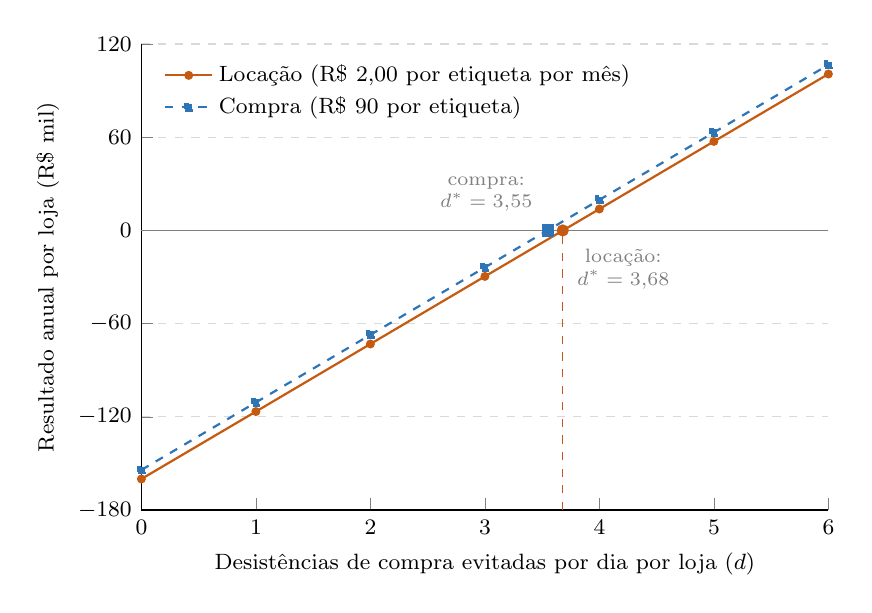
\begin{tikzpicture}
        \begin{axis}[
            r2eixo,
            width=0.85\textwidth, height=7.5cm,
            xmin=0, xmax=6, ymin=-180, ymax=120,
            xtick={0,1,2,3,4,5,6},
            ytick={-180,-120,-60,0,60,120},
            xlabel={Desistências de compra evitadas por dia por loja ($d$)},
            ylabel={Resultado anual por loja (R\$ mil)},
            legend style={at={(0.02,0.98)}, anchor=north west, font=\footnotesize, draw=none, fill=white},
            legend cell align=left,
            clip=false,
        ]
            \draw[r2cinza] (axis cs:0,0) -- (axis cs:6,0);
            \addplot[r2laranja, thick, mark=*, mark size=1.2pt] coordinates {
                (0,-160.0) (1,-116.6) (2,-73.1) (3,-29.6) (4,13.8) (5,57.3) (6,100.7)};
            \addlegendentry{Locação (R\$~2,00 por etiqueta por mês)}
            \addplot[r2azulmedio, thick, dashed, mark=square*, mark size=1.2pt] coordinates {
                (0,-154.2) (1,-110.7) (2,-67.2) (3,-23.8) (4,19.7) (5,63.1) (6,106.6)};
            \addlegendentry{Compra (R\$~90 por etiqueta)}
            \draw[r2laranja, dashed] (axis cs:3.68,-180) -- (axis cs:3.68,0);
            \addplot[only marks, mark=*, mark size=2pt, r2laranja, forget plot] coordinates {(3.68,0)};
            \addplot[only marks, mark=square*, mark size=2pt, r2azulmedio, forget plot] coordinates {(3.55,0)};
            \node[r2rotulo, anchor=north west] at (axis cs:3.72,-6) {locação:\\$d^{*} = 3{,}68$};
            \node[r2rotulo, anchor=south east] at (axis cs:3.50,6) {compra:\\$d^{*} = 3{,}55$};
        \end{axis}
    \end{tikzpicture}
    \source{Elaborado pelos autores (2026). A implantação de R\$~15.000 por loja fica fora de $d^{*}$; a reta da compra não inclui o custo de capital da Riachuelo, com o qual o equilíbrio iria a 4,98.}
\end{figure}

As duas retas têm a mesma inclinação, R\$~43,5 mil por ano por desistência evitada por dia, e diferem só no custo fixo. O equilíbrio também depende do retorno. O contrato de locação prevê uma franquia de perda de 1\% das liberações e, acima dela, cobra R\$~60 por etiqueta não devolvida. Com retorno de 95\%, a cobrança chega a R\$~59.568 por ano e o equilíbrio sobe para 5,05; com 90\%, a R\$~134.028 e 6,77; e com 83\%, o nível do mercado, a R\$~238.272 e 9,16. Nas perdas, o cenário otimista reduz o equilíbrio para 3,42, e o pessimista do ECR 2026 o eleva para 6,58 a 8,32.

Por fim, a equipe calculou o valor econômico de uma liberação para a Riachuelo, a soma dos benefícios dividida pelas 24.820 liberações do ano. Com $d = 2$, esse valor é de R\$~4,07; com $d = 4$, de R\$~7,57; e com $d = 6$, de R\$~11,07. O preço de R\$~7,01 por liberação fica abaixo do valor a partir de $d \approx 3{,}7$, o mesmo ponto de equilíbrio visto pelo lado do preço.

\subsection{Preço e remuneração do fornecedor}
\label{sub:r2-preco}

Do lado do fornecedor, a equipe adotou como premissas o Coletor de Etiquetas a R\$~400, o Liberador de Balcão a R\$~250, a Bandeja de Recarga e a Bancada de Inspeção a R\$~400 cada, o malote a R\$~0,05 por etiqueta por ciclo, a operação e a nuvem a R\$~6.000 por loja por ano e vida de 5 anos sem valor residual. O investimento por loja é de R\$~414.458: a frota de 6.854 etiquetas a R\$~60 (R\$~411.240), 2 Coletores, 5 Liberadores e o rateio do CD, que divide por 20 lojas 17 Bandejas de Recarga e 3 postos de inspeção, cada um com leitor Zebra FXP20 e Bancada de Inspeção (R\$~1.167,78 por loja). Com a receita de R\$~174.096 por ano e custos anuais de reposição de 1\% das liberações (R\$~14.892), recondicionamento (R\$~7.077,56), malote (R\$~1.241) e operação (R\$~6.000), a contribuição anual é de R\$~144.885, o que dá payback de 2,86 anos e TIR de 22,0\% em 5 anos. O custo contábil de uma etiqueta, sem custo de capital, é de R\$~1,28 por mês.

A equipe fixou a taxa mínima de atratividade em 20\% ao ano, premissa formada pela Selic de 15\% \cite{btg2025guararapes} mais 5 pontos percentuais de risco. A R\$~1,80 por etiqueta por mês, a TIR cai para 16,6\%, abaixo da TMA, e esse preço não remunera o capital do fornecedor; a R\$~2,10, a TIR sobe para 24,7\%, e a R\$~2,40, para 32,3\%. O preço mínimo para uma TIR de 20\% é de R\$~1,92. O custo-meta pesa na mesma medida: no limite superior da faixa, R\$~66, a TIR a R\$~2,00 cai para 17,3\%, e no limite inferior, R\$~54, sobe para 27,6\%. Cumprir o custo-meta é, portanto, condição para sustentar o preço de R\$~2,00.

Com essas contas, a equipe definiu o valor mercadológico do Tag\&Go: locação de R\$~2,00 por etiqueta por mês, plataforma de R\$~800 por loja por mês e implantação de R\$~15.000 por loja, com franquia de perda de 1\%; como alternativa, compra a R\$~90 por etiqueta, com recondicionamento a R\$~0,40 por ciclo. A justificativa tem três partes. O preço cobre o custo de capital do fornecedor, com TIR de 22,0\% contra a TMA de 20\%. O preço leva o equilíbrio da Riachuelo a 3,7 desistências evitadas por dia por loja, número plausível diante da desistência por fila registrada no Relatório 1, mas que precisa ser validado no piloto. E o preço fica coerente com a posição do produto na escala vertical, em que o custo-meta se situa entre a ESL e os rastreadores BLE. O preço de compra de R\$~90 equivale ao custo-meta multiplicado por 1,5 e não foi derivado dos vizinhos na escala. A forma de contratação, os canais e a distribuição estão na Seção~\ref{sec:r2-comercializacao}.

No SOM, as 20 lojas conceito do limite superior do plano da Riachuelo para 2026, de 15 a 20 lojas, exigiriam 137.080 etiquetas, uma frota de R\$~8,22 milhões e R\$~300 mil de implantação, com receita de R\$~3,48 milhões por ano para o fornecedor. Estendido às 342 lojas da rede, o mesmo modelo geraria R\$~59,5 milhões por ano.

\subsection{Sensibilidade do equilíbrio e alavancas}
\label{sub:r2-sensibilidade-valor}

Como o equilíbrio depende de premissas ainda não validadas com a Riachuelo, a equipe variou cada uma delas entre um limite favorável e um desfavorável, mantendo as demais no caso base. A Figura~\ref{fig:r2-tornado} ordena as variáveis da faixa mais larga para a mais estreita; a parte da barra abaixo do caso base aparece em azul e a parte acima, em laranja.

\begin{figure}[htbp]
    \centering
    \caption{Sensibilidade do equilíbrio $d^{*}$}
    \label{fig:r2-tornado}
    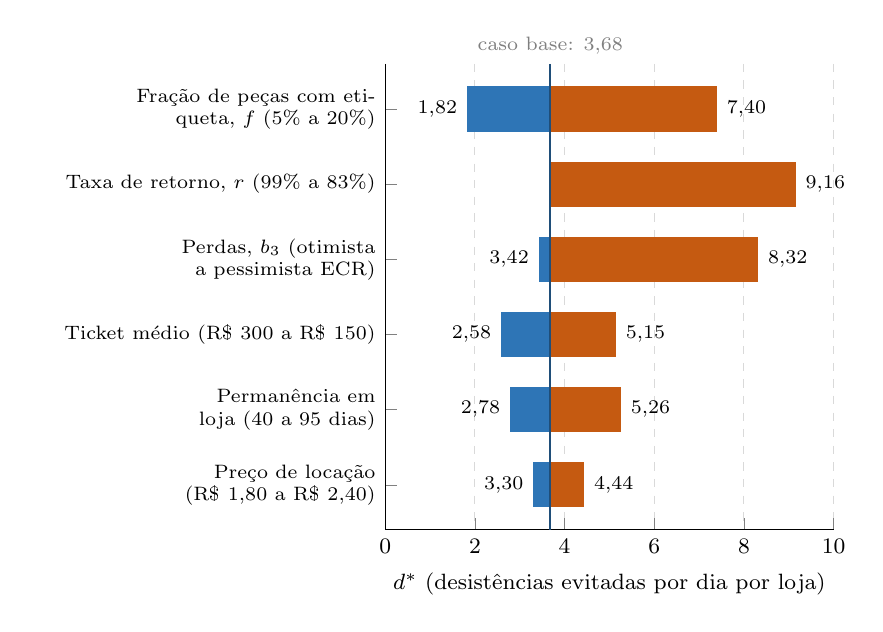
\begin{tikzpicture}
        \begin{axis}[
            r2eixo,
            width=0.6\textwidth, height=7.5cm,
            xmin=0, xmax=10, ymin=0.4, ymax=6.6,
            y dir=reverse,
            ymajorgrids=false, xmajorgrids,
            xtick={0,2,4,6,8,10},
            ytick={1,2,3,4,5,6},
            yticklabels={
                {Fração de peças com etiqueta, $f$ (5\% a 20\%)},
                {Taxa de retorno, $r$ (99\% a 83\%)},
                {Perdas, $b_3$ (otimista a pessimista ECR)},
                {Ticket médio (R\$~300 a R\$~150)},
                {Permanência em loja (40 a 95 dias)},
                {Preço de locação (R\$~1,80 a R\$~2,40)}},
            y tick label style={font=\scriptsize, align=right, text width=4.3cm},
            xlabel={$d^{*}$ (desistências evitadas por dia por loja)},
            clip=false,
        ]
            \fill[r2azulmedio] (axis cs:1.82,0.7) rectangle (axis cs:3.68,1.3);
            \fill[r2laranja] (axis cs:3.68,0.7) rectangle (axis cs:7.40,1.3);
            \node[font=\scriptsize, anchor=east] at (axis cs:1.82,1) {1,82};
            \node[font=\scriptsize, anchor=west] at (axis cs:7.40,1) {7,40};
            \fill[r2laranja] (axis cs:3.68,1.7) rectangle (axis cs:9.16,2.3);
            \node[font=\scriptsize, anchor=west] at (axis cs:9.16,2) {9,16};
            \fill[r2azulmedio] (axis cs:3.42,2.7) rectangle (axis cs:3.68,3.3);
            \fill[r2laranja] (axis cs:3.68,2.7) rectangle (axis cs:8.32,3.3);
            \node[font=\scriptsize, anchor=east] at (axis cs:3.42,3) {3,42};
            \node[font=\scriptsize, anchor=west] at (axis cs:8.32,3) {8,32};
            \fill[r2azulmedio] (axis cs:2.58,3.7) rectangle (axis cs:3.68,4.3);
            \fill[r2laranja] (axis cs:3.68,3.7) rectangle (axis cs:5.15,4.3);
            \node[font=\scriptsize, anchor=east] at (axis cs:2.58,4) {2,58};
            \node[font=\scriptsize, anchor=west] at (axis cs:5.15,4) {5,15};
            \fill[r2azulmedio] (axis cs:2.78,4.7) rectangle (axis cs:3.68,5.3);
            \fill[r2laranja] (axis cs:3.68,4.7) rectangle (axis cs:5.26,5.3);
            \node[font=\scriptsize, anchor=east] at (axis cs:2.78,5) {2,78};
            \node[font=\scriptsize, anchor=west] at (axis cs:5.26,5) {5,26};
            \fill[r2azulmedio] (axis cs:3.30,5.7) rectangle (axis cs:3.68,6.3);
            \fill[r2laranja] (axis cs:3.68,5.7) rectangle (axis cs:4.44,6.3);
            \node[font=\scriptsize, anchor=east] at (axis cs:3.30,6) {3,30};
            \node[font=\scriptsize, anchor=west] at (axis cs:4.44,6) {4,44};
            \draw[r2azul, thick] (axis cs:3.68,0.4) -- (axis cs:3.68,6.6);
            \node[r2rotulo, anchor=south] at (axis cs:3.68,0.4) {caso base: 3,68};
        \end{axis}
    \end{tikzpicture}
    \source{Elaborado pelos autores (2026).}
\end{figure}

As três variáveis mais sensíveis são a fração de peças com etiqueta $f$, a taxa de retorno $r$ e as perdas. A fração $f$ lidera porque o custo da locação cresce com a frota, que é proporcional ao número de liberações, enquanto o benefício por desistência evitada não depende dela: com $f = 5\%$ o equilíbrio cai para 1,82, e com $f = 20\%$ sobe para 7,40. A permanência em loja age pelo mesmo mecanismo, porque aumenta o ciclo $T$ e, com ele, a frota, e leva o equilíbrio de 2,78 (40 dias) a 5,26 (95 dias). O retorno só pode piorar a partir da meta de 99\%, e a queda até o nível do mercado leva o equilíbrio a 9,16. As perdas também têm faixa assimétrica, de 3,42 no cenário otimista a 8,32 no pessimista do ECR 2026. O ticket médio muda o valor de cada desistência evitada e leva o equilíbrio de 2,58 (R\$~300) a 5,15 (R\$~150), e o preço de locação, a variável que o fornecedor controla, tem a faixa mais estreita, de 3,30 a 4,44.

A equipe concluiu, a partir da sensibilidade, que a viabilidade depende mais da forma de uso do sistema que do preço, e identificou quatro alavancas. A primeira é usar o Tag\&Go só nas peças que hoje já recebem etiqueta rígida, de preferência as de maior valor e de giro rápido, o que reduz $f$ e $T$ ao mesmo tempo. A segunda é perseguir o retorno de 99\% com os mecanismos M1 a M4 e acompanhar a taxa por loja desde o primeiro dia do piloto. A terceira é reduzir o custo da etiqueta por \textit{design to cost}, com as cotações de volume previstas para o Relatório 3. A quarta é medir $d$ com a Riachuelo no piloto, porque nenhuma fonte pública consultada pela equipe permite estimar as desistências evitadas para a rede.

\newpage% =============================================================================
% Relatorio 2, item D: estudo de aproveitamento tecnico (projeto Riachuelo).
% Benchmarking por linhas de similaridade (L1 a L8), solucoes descartadas e
% propriedade intelectual (familias conferidas no Google Patents em 25/09/2026).
% Tabela: tab:r2-aproveitamento (longtable). Mapa de posicionamento e vantagens
% comerciais ficam no estudo de diferenciacao (r2/5-diferenciacao.tex).
% =============================================================================

\section{ESTUDO DE APROVEITAMENTO TÉCNICO}
\label{sec:r2-aproveitamento}

O equilíbrio econômico da Seção~\ref{sec:r2-valor} depende de cumprir o custo-meta e de reduzir o risco técnico do desenvolvimento, e as duas coisas ficam mais fáceis quando o sistema reaproveita soluções já testadas em outros produtos.

\subsection{Método}
\label{sub:r2-aprov-metodo}

O estudo de aproveitamento técnico procurou, em produtos análogos, patentes e casos de mercado, soluções já testadas que o sistema Tag\&Go pudesse incorporar em vez de desenvolver do zero. A orientação da disciplina apontou o benchmarking de produtos análogos e de patentes, inclusive no INPI, como a fonte mais útil de princípios de solução e recomendou, em funções como a recomendação de roupas, construir sobre bases existentes \cite{zancul2026conceitual}. A equipe seguiu o precedente de um grupo de anos anteriores da disciplina, o do projeto Carrinho de compras, e organizou a busca por linhas de similaridade: cada linha reúne referências que resolvem um mesmo problema técnico do Tag\&Go, ainda que em outro produto ou em outro setor.

Para cada linha, a equipe listou as referências, extraiu a ideia aproveitável e indicou onde ela entra no sistema, pela função da análise funcional (Tabela~\ref{tab:r2-funcoes}) e pelo subsistema ou componente da arquitetura (Tabela~\ref{tab:r2-ssc}). O critério de aproveitamento foi técnico: a ideia precisava realizar uma função do Tag\&Go, ser compatível com as especificações-meta e com o envelope herdado do Relatório 1 e não depender de recurso sem precedente comercial. As oito linhas resultantes, L1 a L8, cobrem a etiqueta e sua liberação (L1, L2, L3 e L5), o pagamento (L4), a loja (L6), o ciclo logístico (L7) e a Jornada Completa (L8), e estão consolidadas na Tabela~\ref{tab:r2-aproveitamento}. O mapa de posicionamento e as vantagens comerciais frente às mesmas referências pertencem ao estudo de diferenciação (Seção~\ref{sec:r2-diferenciacao}); o aproveitamento técnico trata apenas do que cada referência ensina sobre como realizar as funções. As ideias aproveitadas alimentaram os princípios de solução e a matriz morfológica da Seção~\ref{sec:r2-concepcao}.

\subsection{Linhas de similaridade}
\label{sub:r2-aprov-linhas}

A primeira linha, retenção mecânica (L1), partiu das etiquetas rígidas comerciais e da garra e do pino retirados de mini tags doadoras no protótipo do Relatório 1. Essas etiquetas usam uma embreagem de três esferas num copo cônico, em que a retenção cresce com a força de extração: quanto mais se puxa o pino, mais as esferas apertam a haste. Esse autotravamento dispensa energia para reter a peça, o que é decisivo para uma etiqueta que passa a maior parte do ciclo parada no estado TRAVADA. A equipe aproveitou a garra (\O\,12,4 $\times$ 10\,mm, curso de 1,2\,mm e mola estimada em 2,5\,N, valores a medir), o pino padrão do mercado, com cabeça de \O\,14\,mm e haste de \O\,2,0\,mm, e o elemento EAS da mini tag, que mantém a compatibilidade com os pórticos EAS já instalados nas lojas. O pino padrão preserva, além disso, o gesto de aplicação que já é conhecido de quem etiqueta peças, o que simplifica o cadastro na origem. A única mudança na garra é o carretel não ferromagnético, que impede a abertura pelo destacador comercial (especificação E11). A linha entra nas funções reter peça (F1) e sinalizar saída indevida (F12) e nos componentes C1.3 (garra), C1.4 (pino) e C1.10 (elemento EAS). A meta de resistência à extração de pelo menos 120\,N (E02) é da equipe e ainda será comparada, em ensaio, com a de uma etiqueta comercial.

A segunda linha, liberação autorizada (L2), reuniu dispositivos que só soltam a peça depois de uma verificação. A patente US 7.450.013 B2, da Checkpoint, expirada em 2025 e hoje em domínio público \cite{googlepatents2008us7450013}, descreve um destacamento autenticado que depende de condições controladas, como um ímã propositalmente forte e uma velocidade calibrada, e prevê uma posição sem energia que permite a liberação de emergência. A SuperTag 4, da Sensormatic, confere se o item pago corresponde ao da etiqueta antes de acionar o destacador motorizado do self-checkout e, segundo o fornecedor, só destaca com compra válida \cite{sensormatic2026supertag}. A patente US 11.417.186 B2, da Kohl's, automatiza a retirada e deixa as etiquetas caírem em caixas coletoras \cite{googlepatents2022us11417186}, e as travas LIVE Locks, da InVue, abertas pelo celular, registram cada abertura por loja, departamento e usuário \cite{invue2026locks}. Dessas referências a equipe tirou quatro ideias. A primeira é que toda etiqueta precisa de um caminho de liberação independente da própria bateria: no Tag\&Go, o Liberador de Balcão energiza a etiqueta pelos contatos da face superior e entrega a autorização por eles. A segunda é a conferência entre etiqueta e item, feita pela associação entre o \texttt{tag\_id} e o EPC da peça na Estação de Cadastro, de modo que o preço venha sempre do EPC. A terceira é a queda por gravidade numa caixa trancada, que originou o Coletor de Etiquetas com boca antirretorno. A quarta é a trilha de auditoria, convertida na meta de registrar 100\% das emissões de token e das liberações (S10). A linha entra nas funções validar autorização (F5), oferecer liberação assistida (F16), recolher etiqueta (F17) e associar etiqueta à peça (F21) e nos componentes C1.5 (atuador), C4.1 (Coletor de Etiquetas) e C4.2 (Liberador de Balcão).

A terceira linha, identificação e leitura pelo celular (L3), tratou do caminho entre a peça e o canal de compra. A Apple documenta que o iPhone XS e os modelos posteriores leem NFC em segundo plano e, quando o primeiro registro NDEF traz um universal link, abrem o app ou o App Clip associado; sem app associado, abrem o Safari \cite{apple2026corenfc}. O App Clip Code combina código visual e NFC, mas a versão com NFC exige uma etiqueta NFC Type 5 de pelo menos 35\,mm \cite{apple2026appcliphig}, maior que a área disponível sob o QR de 28\,mm. O NTAG 424 DNA, da NXP, gera com AES-128 uma mensagem autenticada diferente a cada toque, o que impede copiar a URL \cite{nxp2026ntag424}. A equipe aproveitou a combinação de QR impresso e NFC com a mesma URL, que contém apenas o identificador público e estável da etiqueta; a peça atual vem da Plataforma Tag\&Go a cada leitura. A cópia da URL, por si só, não libera nenhuma peça, porque a liberação depende do token verificado na etiqueta (Seção~\ref{sec:r2-arquitetura}). Ainda assim, a equipe registrou o NTAG 424 DNA como evolução, caso a clonagem de URLs se mostre um problema na operação. A linha entra na função identificar peça (F2) e no componente C1.9 (identificação).

A quarta linha, pagamento sem app (L4), buscou formas de pagar sem instalar um aplicativo. Na Flying Tiger, a MishiPay oferece scan and go num web app aberto por QR, sem baixar app, e relata cesta 35\% maior, segundo o fornecedor \cite{mishipay2026flyingtiger}. Na apresentação dos App Clips na WWDC20, a Apple mostrou um toque numa etiqueta NFC que abre o App Clip na página de pedido e uma compra concluída com Apple Pay \cite{apple2020wwdcappclips}. Na web, a biblioteca JavaScript da Google Pay API permite pagar sem instalar app, desde que haja um processador de pagamento (PSP) \cite{google2026paywebvisao}. O Pix completa o conjunto: no recorte brasileiro de uma pesquisa da Adyen, com amostra não informada, 60\% dos consumidores disseram desistir da compra quando não podem pagar como querem \cite{tiinside2026adyen}. A equipe aproveitou esses elementos na Compra Rápida (Subseção~\ref{sub:r2-caminhos}): o App Clip Tag\&Go no iPhone e a Página de Compra Rápida no Android pagam pela carteira digital, com um toque no botão da carteira e confirmação por Face ID, Touch ID ou senha na folha do sistema, e oferecem o Pix copia e cola como alternativa. A linha entra na função processar pagamento (F3) e nos componentes C3.1 (App Clip Tag\&Go) e C3.2 (Página de Compra Rápida).

A quinta linha, energia e recarga (L5), comparou dispositivos que dependem de bateria ou de energia externa. As etiquetas eletrônicas de prateleira (ESL) da Vusion e da SOLUM são o precedente mais próximo de um dispositivo com bateria e rádio instalado em grande número no salão de venda \cite{vusion2026esl,solum2026esl}, e as travas da InVue anunciam bateria de dois anos \cite{invue2026locks}. A patente US 10.497.238 B2, da Sensormatic, descreve uma estação que energiza uma etiqueta sem bateria no momento da liberação \cite{googlepatents2019us10497238}. Os estudos anteriores da equipe mostraram, por um balanço de energia, que o gargalo de uma etiqueta sem bateria é a potência instantânea, e não a energia total: a RF ambiente, de cerca de 5\,$\mu$W, levaria cerca de 35\,h para acumular a energia de uma liberação com fio SMA; um campo NFC dedicado, de cerca de 6\,mW, cerca de 105\,s; e contatos de 5\,W, cerca de 1,5\,s. Dessas referências a equipe tirou três ideias: recarregar a célula por contatos, numa Bandeja de Recarga no CD, sem conectar cabos a cada etiqueta; manter a etiqueta em sono profundo e acordá-la só pelo botão (modo botão), o que dá autonomia de 448 dias com a célula de 150\,mAh, estimativa da equipe, contra a meta de 168 dias (E05); e fornecer energia externa pelo Liberador de Balcão quando a célula falhar. A linha entra nas funções armazenar energia (F7), repor energia (F8) e oferecer liberação assistida (F16) e nos componentes C1.7 (célula), C4.2 (Liberador de Balcão) e C5.3 (Bandeja de Recarga).

A sexta linha, localização e estoque (L6), comparou formas de informar ao cliente onde está a peça. O Store Mode da Zara mostra no mapa da loja onde a peça está exposta \cite{inditex2021storemode}; o app do Walmart marca o corredor num mapa em mais de 4.700 lojas \cite{walmart2019mapas}; e a Renner atualiza o estoque RFID a cada 60\,s \cite{infomoney2024renner}. Para maior precisão, o leitor de teto Impinj xArray localiza 85\% das etiquetas a até 1,5\,m em condição ideal, mas está em fim de vida e tem preço sob consulta \cite{atlasrfid2026xarray}, e uma solução comercial de Bluetooth com ângulo de chegada, citada pelo Bluetooth SIG, tem erro médio de 1 a 2\,m \cite{bluetooth2022direction}. A rapitag usou um algoritmo que achava pelo BLE o produto mais próximo do celular \cite{storesshops2019rapitag}, e as ESLs da Vusion têm LED de sete cores para guiar a separação e o cliente \cite{vusion2026esl}. Como localizar o produto na loja é uma função secundária acessória, a decisão foi de granularidade, entre o nível N0, da unidade, e o nível N3, da peça, e a escolha está na análise funcional (Tabela~\ref{tab:r2-granularidade}). A equipe aproveitou o nível N1, por setor, a partir do estoque RFID que a Riachuelo já opera e de um planograma digital mantido pela loja, como na Zara e no Walmart, e registrou o nível N2, por arara ou expositor, como evolução caso a Riachuelo instale leitores de teto. A ideia da rapitag não foi levada à etiqueta, porque o anúncio BLE contínuo esgotaria a célula antes do fim de um ciclo (Subseção~\ref{sub:r2-localizar}). A linha entra nas funções localizar produto na loja (F25) e informar disponibilidade (F26) e no serviço Jornada (C2.5).

A sétima linha, logística reversa (L7), estudou ativos retornáveis do varejo. A Sensormatic recircula etiquetas rígidas: as etiquetas e os pinos retirados no caixa são encaixotados, voltam aos CDs no retorno dos caminhões (\textit{back-haul}), são testados, limpos, separados, reembalados e enviados às fábricas de roupa; desde 2010, segundo o fornecedor, 16,5 bilhões de etiquetas foram enviadas e 13,7 bilhões recirculadas \cite{sensormatic2024recirculacao}, razão de cerca de 83\% calculada pela equipe. A Pact informa que suas etiquetas EAS reutilizáveis fazem no mínimo 8 a 10 viagens, com reuso de até 80\% \cite{pact2026etiquetas}, e a Inditex contratou a Tyco em 2014 para recircular etiquetas rígidas com RFID e AM em três a quatro centros, com apagamento do identificador \cite{rfidjournal2014inditex}. Nos cabides, a Braiform estima que reusar um cabide nove vezes reduz 79\% das emissões \cite{braiform2018cabides}, e a Mainetti opera o reuso desde meados dos anos 1980 \cite{mainetti2018cabides}. A Brambles, que opera paletes em pool, mostra que a taxa de perda do ativo retornável domina a economia do sistema \cite{brambles2025resultados}, e a Decathlon aplica o RFID na fábrica em 600 milhões de produtos por ano \cite{rfidnews2026decathlon}. A equipe aproveitou o Malote de Retorno no retorno do caminhão da frota própria, a Bancada de Inspeção no CD, o cadastro na origem, feito na Estação de Cadastro nos ramos fábrica e CD como no \textit{source tagging} da Decathlon, e um indicador de perda por loja, que acompanha a meta de retorno de 99\% (S01), acima da faixa de 80\% a 83\% observada no mercado. O Tag\&Go recircula uma etiqueta com bateria e chave criptográfica, o que acrescenta ao ciclo a recarga e as regras de transporte de baterias de lítio (Subseção~\ref{sub:r2-ciclo}); o efeito da taxa de retorno sobre a economia do sistema foi tratado na Seção~\ref{sec:r2-valor}. A linha entra nas funções F17 a F24 e no subsistema SS5 (ciclo logístico).

A oitava linha, jornada, fidelidade e dados (L8), reuniu referências para as funções da Jornada Completa. O Nike App at Retail reconhece o membro na loja, lê o produto para mostrar cores e tamanhos disponíveis, reserva peças para provar e permite pagar sem fila \cite{marketingdive2018nike}. A Sephora organiza a fidelidade em três níveis por gasto anual \cite{modernretail2024sephora}. O ``Complete the Look'' da Zalando aumentou em 25\% as interações com looks de criadores em dois meses \cite{zalando2021looks}, e a Stitch Fix combina filtragem colaborativa, similaridade visual e um stylist humano na seleção final \cite{stitchfix2026algoritmos}. A Renner usa algoritmos que comparam produtos por imagem e recomendação por transações \cite{infomoney2024renner}. Do lado da Riachuelo, o Ria Club já paga cashback de 12\% com o cartão Riachuelo e de 10\% nos demais meios \cite{midway2026riaclub}. O Apple Wallet aceita passes de fidelidade distribuídos pela web, por QR, por NFC ou por App Clip, e o Google Wallet emite cartões de fidelidade por link, ambos sem exigir o app do varejista \cite{apple2026walletpass,google2026walletfidelidade}. Seguindo a orientação de construir a recomendação sobre bases existentes \cite{zancul2026conceitual}, a equipe aproveitou quatro ideias: um modelo híbrido de recomendação (regras de coleção, filtragem colaborativa e similaridade visual, com looks de stylists) restrito ao que existe na loja no tamanho do perfil; o botão ``chamar vendedor'', que preserva o atendimento humano; o passe do Ria Club no Wallet, oferecido depois da Compra Rápida; e o cashback liberado só depois do registro de ``etiqueta devolvida'', que liga a fidelidade à meta de retorno. As demais funções da Jornada Completa, como a compra on-line do tamanho ausente e as métricas de sustentabilidade por categoria, seguem a Subseção~\ref{sub:r2-caminhos}. Essas funções continuam hipóteses, porque o survey do Relatório 1 não mediu interesse por fidelidade, recomendação ou sustentabilidade. A linha entra nas funções acionar atendimento humano (F15) e F27 a F31 e nos componentes C2.5 (Jornada), C3.3 (módulo Tag\&Go do app Riachuelo) e C3.4 (passe do Ria Club).

A partir das oito linhas, a equipe concluiu que quase todas as funções do Tag\&Go têm precedente comercial isolado: a retenção vem das etiquetas rígidas, a leitura e o pagamento sem app vêm das plataformas móveis, a recirculação vem da Sensormatic e da Pact, e a localização por setor vem da Zara e do Walmart. O desenvolvimento próprio fica concentrado na integração dessas soluções e em dois pontos para os quais a equipe não encontrou solução pronta para aproveitar: a verificação do token na própria etiqueta, com desafio gerado por ela, e a recirculação de uma etiqueta com bateria e chave criptográfica. A Tabela~\ref{tab:r2-aproveitamento} consolida as linhas, as ideias aproveitadas e o lugar de cada uma no sistema, com as funções da Tabela~\ref{tab:r2-funcoes} e os componentes da Tabela~\ref{tab:r2-ssc}.

\begingroup
\footnotesize
\setlength{\tabcolsep}{4pt}
\renewcommand{\arraystretch}{1.25}
\begin{longtable}{@{}
    >{\RaggedRight\arraybackslash}p{2.2cm}
    >{\RaggedRight\arraybackslash}p{5.3cm}
    >{\RaggedRight\arraybackslash}p{4.6cm}
    >{\RaggedRight\arraybackslash}p{2.5cm}@{}}
\caption{Linhas de similaridade e ideias aproveitadas} \label{tab:r2-aproveitamento} \\
\toprule
\textbf{Linha} & \textbf{Referências} & \textbf{Ideia aproveitada} & \textbf{Onde entra} \\
\midrule
\endfirsthead
\multicolumn{4}{c}{Tabela~\ref{tab:r2-aproveitamento} (continuação)} \\
\toprule
\textbf{Linha} & \textbf{Referências} & \textbf{Ideia aproveitada} & \textbf{Onde entra} \\
\midrule
\endhead
\midrule
\multicolumn{4}{r}{\textit{continua na próxima página}} \\
\endfoot
\bottomrule
\multicolumn{4}{c}{Fonte: Elaborado pelos autores (2026) com base nas fontes citadas no texto.} \\
\endlastfoot
L1 Retenção mecânica & etiquetas rígidas comerciais; garra e pino retirados de mini tags no protótipo do Relatório 1 & embreagem de 3 esferas com copo cônico, pino padrão do mercado e elemento EAS de mini tag: compatibilidade com a operação atual e com os pórticos & F1, F12; C1.3, C1.4, C1.10 \\
\addlinespace
L2 Liberação autorizada & US 7.450.013 B2 (Checkpoint, domínio público desde 2025): ímã propositalmente forte, velocidade calibrada e posição sem energia que permite liberação de emergência; SuperTag 4: conferência item-etiqueta; Kohl's US 11.417.186 B2: retirada automática com queda em caixas coletoras; InVue: trilha de auditoria & liberação de emergência pelo Liberador de Balcão; conferência etiqueta-EPC; Coletor de Etiquetas com queda por gravidade; registro de toda liberação (S10) & F5, F16, F17, F21; C1.5, C4.1, C4.2 \\
\addlinespace
L3 Identificação e leitura pelo celular & NFC com universal link e QR (Apple); App Clip Code; NTAG 424 DNA (mensagem autenticada a cada toque) & mesma URL no QR e no NFC; evolução para NFC com mensagem autenticada se houver clonagem de URL & F2; C1.9 \\
\addlinespace
L4 Pagamento sem app & MishiPay (web app por QR na Flying Tiger); Apple Pay em App Clip (WWDC20); Google Pay API na web; Pix & Compra Rápida por App Clip e página; carteira com um toque e confirmação por Face ID, Touch ID ou senha; Pix copia e cola como alternativa & F3; C3.1, C3.2 \\
\addlinespace
L5 Energia e recarga & ESLs com bateria e rádio (Vusion, SOLUM); InVue (bateria de 2 anos); US 10.497.238 B2 (estação que energiza etiqueta sem bateria); balanço de energia dos estudos anteriores da equipe & recarga por contatos em bandeja no CD; modo de sono profundo; energia externa no Liberador de Balcão & F7, F8, F16; C1.7, C4.2, C5.3 \\
\addlinespace
L6 Localização e estoque & Zara Store Mode (planta); Walmart (corredor); Renner (estoque RFID a cada 60\,s); xArray; BLE com ângulo de chegada; rapitag (produto mais próximo pelo BLE); ESLs com LED & N1 por estoque RFID e planograma; N2 como evolução com leitores de teto & F25, F26; C2.5 \\
\addlinespace
L7 Logística reversa & Sensormatic (\textit{back-haul}, teste, limpeza, envio às fábricas); Pact (8 a 10 viagens; reuso de até 80\%); Inditex e Tyco (3 a 4 centros; apagamento do identificador); cabides Braiform e Mainetti; Brambles (a perda domina o custo); Decathlon (RFID na fábrica) & Malote de Retorno no retorno do caminhão; Bancada de Inspeção; cadastro na origem; indicador de perda por loja & F17 a F24; SS5 \\
\addlinespace
L8 Jornada, fidelidade e dados & Nike App at Retail; Sephora (níveis por gasto); Zalando (Complete the Look); Stitch Fix (algoritmo e stylist); Renner (CRM e IA); Ria Club; passes do Wallet & recomendação híbrida restrita ao estoque; botão ``chamar vendedor''; passe do Ria Club sem app; cashback após ``etiqueta devolvida'' & F15, F27 a F31; C2.5, C3.3, C3.4 \\
\end{longtable}
\endgroup

\subsection{Soluções descartadas}
\label{sub:r2-aprov-descartadas}

O estudo também registrou as soluções que a equipe decidiu não aproveitar, para que a decisão fique rastreável nas etapas seguintes do projeto. Quatro delas foram descartadas por evidência de uso ou de regulação. A visão computacional, base de parte das lojas sem caixa, não serve bem a roupas: a Amazon passou a usar RFID no Just Walk Out para vestuário porque a visão computacional exige produtos em prateleira \cite{amazon2024jwo}. O alarme sem barreira física também foi descartado, porque a Zara atrasou em 2023 a implantação de um sistema RFID sem etiqueta rígida, já que os chips eram fáceis de arrancar e o alarme tocava em devoluções \cite{pymnts2023zara}, e porque testes de retirada de etiquetas rígidas relatados pela Sensormatic, parte interessada, registraram aumento de perda de 40\% a mais que o dobro \cite{sensormatic2024hardtag}. O pagamento facial próprio, como o oferecido pela C\&A aos clientes do C\&A Pay \cite{mobiletime2023cea}, exigiria tratar dado biométrico, que a LGPD classifica como sensível (art.~11) \cite{brasil2018lgpd}; na carteira digital, a biometria fica no aparelho do cliente e não chega à Riachuelo. O Pix por aproximação, por fim, não se aplica, porque a etiqueta não é terminal de pagamento; o recurso começou em 2025, só no Android com Google Pay \cite{agenciabrasil2025pix}.

As outras cinco foram descartadas por limitação física, de escala ou de protótipo. A colheita de RF ambiente levaria cerca de 35\,h por liberação, segundo o balanço de energia dos estudos anteriores da equipe. Uma porta USB em cada etiqueta obrigaria a conectar à mão, uma a uma, as etiquetas da frota, o que não escala no recondicionamento. O anúncio BLE contínuo, a cada 1\,s, esgotaria a célula de 150\,mAh em cerca de 16 dias, estimativa da equipe, menos que um ciclo de 84 dias. O leitor UHF próprio no protótipo foi descartado porque o módulo avaliado, de US\$~79, não tem venda no Brasil (estudos anteriores da equipe); em escala, a leitura do EPC fica com o leitor da Estação de Cadastro e com a infraestrutura RFID que a Riachuelo já opera. O destacador magnético, por fim, foi substituído pelo carretel não ferromagnético e pelo Liberador de Balcão, porque desacopladores de 10.000\,GS são vendidos livremente por cerca de R\$~300 \cite{canalautomacao2026desacoplador} e abririam qualquer etiqueta com carretel ferromagnético.

\subsection{Propriedade intelectual}
\label{sub:r2-aprov-patentes}

A equipe fez a busca de patentes no Google Patents em 25/09/2026, a partir das referências das linhas L2 e L5, e conferiu a família de cada documento. O documento mais próximo do Tag\&Go é a patente US 10.121.339 B2, da Sensormatic (antiga Tyco), com prioridade em 04/03/2015, concedida em 06/11/2018 e ativa até 21/10/2035 \cite{googlepatents2018us10121339}. Sua reivindicação 1 descreve um celular, uma compra verificada, um comando sem fio e um pino liberado sem ajuda humana, conjunto muito próximo da concepção A1 Etiqueta Ativa. A família inclui os documentos CN107667395 (A e B), EP3265631 (A1 e B1), ES2746916T3, WO2016141039A1, US10121338B2 e US10522016B2, além de pedidos nos Estados Unidos, sem nenhuma publicação brasileira.

Outras três famílias ativas tratam da retirada de etiquetas depois do pagamento ou da energia na liberação. A US 10.354.507 B1, da Mastercard, descreve uma estação que remove a etiqueta depois de verificar o pagamento \cite{googlepatents2019us10354507}, e as US 11.417.186 B2 e US 11.984.003 B2, da Kohl's, descrevem a retirada automática de etiquetas \cite{googlepatents2022us11417186}; as duas famílias têm documentos só nos Estados Unidos. A US 10.497.238 B2, da Sensormatic, descreve a estação que energiza uma etiqueta sem bateria e tem família na China, na Europa, em Hong Kong e na Coreia do Sul, também sem publicação brasileira \cite{googlepatents2019us10497238}. Duas patentes da Checkpoint já expiraram: a US 7.450.013 B2, em 2025, hoje em domínio público e aproveitada na linha L2 \cite{googlepatents2008us7450013}, e a US 7.564.360 B2, que descreve um atuador dentro da etiqueta acionado por um sinal de liberação aberto, isto é, sem autenticação \cite{googlepatents2009us7564360}.

Em relação à US 10.121.339 B2, a solução do Tag\&Go difere em quatro pontos técnicos. O desafio (nonce) é gerado pela própria etiqueta, e o token é verificado nela mesma, com HMAC e chave por etiqueta, sem consulta à Plataforma Tag\&Go no momento da validação, de modo que o celular apenas retransmite e não carrega segredo. A associação entre etiqueta e EPC é feita na origem, e o pórtico RFID fecha a malha antifraude ao alarmar quando sai um EPC não vendido. A liberação assistida acontece por contatos, no Liberador de Balcão, mesmo com a célula descarregada. Por fim, os dois caminhos de uso, Compra Rápida e Jornada Completa, compartilham o mesmo núcleo comum. Essa comparação descreve diferenças de solução e não constitui parecer de liberdade de operação.

Como a proteção patentária é territorial, a equipe registrou apenas o que encontrou na consulta: nenhuma das famílias ativas tem publicação brasileira no Google Patents. Essa ausência ainda precisa ser confirmada no INPI, porque a fase nacional de um pedido internacional (PCT), como o WO2016141039A1 da família da US 10.121.339 B2, pode não aparecer no Google Patents. O efeito dessas famílias sobre fabricar e vender no Brasil, ou sobre exportar para os países em que elas existem, depende dessa confirmação e de uma análise jurídica que não faz parte deste relatório. A busca no INPI ficou como tarefa do Relatório 3, sob responsabilidade da dupla que elaborou este estudo. O risco tem precedente no varejo de moda: segundo os estudos anteriores da equipe, a Asterisk processou a Fast Retailing no Japão pela caixa de leitura RFID do self-checkout da Uniqlo e venceu a disputa em 2021.

\newpage% =============================================================================
% Relatorio 2, Secao 6: principios de solucao e alternativas de concepcao
% (item E do roteiro, parte 1). Conteudo: efeitos fisicos e portadores
% (tab:r2-efeitos), matriz morfologica (tab:r2-morfologica), alternativas A1 a
% A3, filtro eliminatorio EC1 a EC3, matriz de decisao (tab:r2-decisao) e
% sensibilidade ao peso do varejista (fig:r2-sensibilidade-matriz).
% Numeros da matriz e custos por loja: script canonico conta_final.py.
% Nao repete SSCs, desenhos, fluxos nem contas de preco (Secoes 4 e 7).
% =============================================================================

\section{PRINCÍPIOS DE SOLUÇÃO E ALTERNATIVAS DE CONCEPÇÃO}
\label{sec:r2-concepcao}

As ideias reunidas no estudo de aproveitamento técnico, somadas às funções da Seção~\ref{sec:r2-funcional}, que descrevem o que o sistema Tag\&Go deve fazer sem dizer como, formaram a base para escolher os meios. A reformulação dos desenhos pedida no roteiro da disciplina começou pela escolha desses meios: para cada função que depende de uma decisão física ou lógica, a equipe levantou os princípios de solução possíveis, combinou-os numa matriz morfológica, montou três alternativas de concepção e escolheu uma delas por um filtro eliminatório seguido de uma matriz de decisão ponderada, com análise de sensibilidade dos pesos \cite{zancul2026conceitual}. A arquitetura, os componentes e o desenho da concepção escolhida ficaram para a Seção~\ref{sec:r2-arquitetura}, e a viabilidade econômica, para a Seção~\ref{sec:r2-valor}.

\subsection{Efeitos físicos e portadores}

Segundo \citeonline{rozenfeld2006gestao}, um princípio de solução reúne um efeito físico, que explica por que a função pode ser cumprida, e um portador desse efeito, que é a forma concreta pela qual ele se manifesta no produto. A equipe aplicou essa decomposição às funções da Tabela~\ref{tab:r2-funcoes} cujo cumprimento depende de uma escolha de princípio, isto é, às funções da etiqueta, da comunicação entre etiqueta e celular, da sinalização e da coleta. As funções que se resolvem por serviços de software e por processos logísticos, como registrar a venda no estoque, emitir o comprovante, rastrear a frota e as funções do ciclo da etiqueta, não mudam de uma alternativa para outra e foram deixadas para a arquitetura. O mesmo vale para as funções da Jornada Completa (F26 a F31), serviços de software do módulo Tag\&Go do app Riachuelo, iguais nas três alternativas. Processar pagamento (F3) também não tem efeito físico próprio: seus portadores são os meios de pagamento, listados na própria matriz morfológica. O resultado do levantamento está na Tabela~\ref{tab:r2-efeitos}.

\begin{table}[htbp]
    \centering
    \caption{Efeitos físicos e portadores considerados por função}
    \label{tab:r2-efeitos}
    \footnotesize
    \renewcommand{\arraystretch}{1.25}
    \begin{tabularx}{\textwidth}{@{}
        >{\RaggedRight\arraybackslash}p{3.3cm}
        >{\RaggedRight\arraybackslash}p{4.6cm}
        >{\RaggedRight\arraybackslash}X@{}}
        \toprule
        \textbf{Função} & \textbf{Efeito físico (o que faz)} & \textbf{Portadores considerados (como faz)} \\
        \midrule
        F1 Reter peça & autotravamento por cunha e atrito & esferas em copo cônico com mola (garra comercial); trava de pino com mola lateral; trava magnética bipolar proprietária \\
        \addlinespace
        F6 Desfazer retenção (deslocar o carretel 1,2\,mm) & conversão de movimento por plano inclinado; força eletromagnética; memória de forma; força magnética externa & came com cursor de rampa (servo ou micromotor); fuso; solenoide; fio SMA com rampa; eletroímã na gaiola; ímã do destacador \\
        \addlinespace
        F7 Armazenar energia & eletroquímica; eletrostática & célula LiPo recarregável; supercapacitor; pilha primária \\
        \addlinespace
        F8 Repor energia & condução; indução eletromagnética; radiação de RF & contatos (Bandeja de Recarga e Liberador de Balcão); indução (Qi); campo NFC; RF ambiente \\
        \addlinespace
        F9 Transmitir autorização & ondas de rádio de 2,4\,GHz; acoplamento indutivo de 13,56\,MHz; condução & BLE (GATT); NFC (Web NFC ou Core NFC); UART por contatos; rede da loja até uma estação \\
        \addlinespace
        F2 Identificar peça & reflexão óptica; acoplamento indutivo; retroespalhamento UHF & QR impresso; NFC NTAG213; EPC RFID da peça; código de barras EAN-13 (não serializa a unidade) \\
        \addlinespace
        F4 e F5 Emitir e validar autorização & função criptográfica (princípio lógico, não físico) & HMAC-SHA256 com chave por etiqueta; assinatura ECDSA; consulta on-line numa estação; código fixo \\
        \addlinespace
        F10 Confirmar intenção de liberar & contato mecânico; proximidade & botão na etiqueta; toque na tela; aproximação a uma estação \\
        \addlinespace
        F11 Indicar estado da liberação & emissão de luz; som; imagem em tela & LED RGB com padrões; buzzer piezo; tela do celular; display da estação \\
        \addlinespace
        F12 Sinalizar saída indevida & ressonância acustomagnética; ressonância LC; retroespalhamento UHF & elemento AM de 58\,kHz; elemento RF de 8,2\,MHz; EPC não vendido lido no pórtico RFID \\
        \addlinespace
        F17 Recolher etiqueta & gravidade e geometria & Coletor de Etiquetas com boca antirretorno; caixa coletora no caixa; queda dentro de uma estação \\
        \addlinespace
        F25 Localizar produto na loja & intensidade de sinal; ângulo de chegada; tempo de voo; proximidade RFID & níveis N0 a N3 da Tabela~\ref{tab:r2-granularidade}; a própria etiqueta como farol BLE \\
        \bottomrule
    \end{tabularx}
    \source{Elaborado pelos autores (2026) com base em \citeonline{rozenfeld2006gestao}.}
\end{table}

Na retenção e na liberação (F1 e F6), a equipe partiu da garra comercial de três esferas, que trava por cunha e atrito e retém mais quanto maior a força de extração, e comparou os atuadores capazes de deslocar o carretel em 1,2\,mm contra a mola. A comparação, feita em estudos anteriores da equipe com o modelo paramétrico do dispositivo do Relatório 1 e atrito estimado de 0,30, deu ao came com servo e braço de 20\,mm uma força de 76,4\,N no carretel, margem de 30,6 vezes sobre a mola e 0,4\,s de acionamento; ao fuso com micromotor, 68,7\,N, margem de 27,5 vezes e 1,6\,s; ao solenoide, 7,6\,N e margem de 3,0 vezes, no limite da meta E04; ao fio SMA, 5,0\,N, margem de 2,0 vezes e cerca de 10\,s para esfriar entre acionamentos; e ao eletroímã, 3,0\,N e margem de 1,2 vez. Nos mesmos estudos, a equipe verificou que o fio SMA precisa de 42\,mm retos atrás do cursor, onde há 5\,mm, e que o eletroímã exigiria uma altura de 30,8\,mm, contra os 26\,mm do envelope. A força magnética externa, por fim, é o princípio do destacador comum e só faz sentido numa concepção em que a etiqueta não tenha eletrônica.

Na energia (F7 e F8), a equipe concluiu, pelo balanço de energia dos estudos anteriores, que o gargalo é a potência instantânea, e não a energia total de uma liberação. A radiação de RF ambiente, de cerca de 5\,$\mu$W, levaria cerca de 35\,h para acumular a energia de uma liberação com SMA; um campo NFC dedicado, de cerca de 6\,mW, levaria cerca de 105\,s; contatos ou indução de 5\,W, cerca de 1,5\,s. Por isso, as alternativas que dispensam bateria dependem de um ponto de energização ou aceitam uma espera longa. Quando há célula, o modo de espera decide a viabilidade: com a célula de 150\,mAh, a etiqueta que só acorda pelo botão dura cerca de 448 dias em espera, e a que anuncia por BLE a cada segundo dura 16 dias (estimativas da equipe, com autodescarga de 3\% ao mês), contra a meta E05 de 168 dias.

Na identificação e na transmissão da autorização (F2 e F9), os portadores foram filtrados pelo que o celular do cliente consegue ler e transmitir. O QR é lido pela câmera de qualquer celular recente, e o NFC, pelos iPhones a partir do XS e pelos aparelhos Android com NFC \cite{apple2026corenfc}, ao passo que o EPC da peça, gravado em RFID UHF, não é lido pelo celular, e o código EAN-13 identifica só o modelo, sem distinguir a unidade. Para a autorização, o BLE só está disponível na web pelo Web Bluetooth, que existe no Chrome para Android e no Samsung Internet e não existe em nenhum navegador do iPhone \cite{chrome2026webbluetooth,caniuse2026webbluetooth}; o Web NFC existe só no Chrome para Android \cite{chrome2026webnfc}. No iPhone, o caminho sem instalar app passa pelo App Clip, e o Core Bluetooth não aparece na lista de frameworks sem função no App Clip \cite{apple2026appclipfuncoes}; a Apple respondeu no fórum oficial que App Clips podem usar Bluetooth, sem trabalhar em segundo plano \cite{apple2020forumble}. O uso de Core Bluetooth no App Clip é, portanto, uma dedução da documentação, que o protótipo precisará confirmar.

A autorização (F4 e F5) tem um princípio lógico. O código fixo foi descartado de saída, porque quem o copia uma vez libera a etiqueta sempre, o que viola R06. A consulta on-line exige que o ponto de liberação esteja ligado à rede da loja, o que só cabe numa estação. Entre as assinaturas verificadas na própria etiqueta, a equipe preferiu o HMAC-SHA256 com chave por etiqueta, porque o ESP32-C3 tem um periférico HMAC em hardware que calcula o código com a chave guardada em eFuse protegido contra leitura, sem expô-la ao software \cite{espressif2026esp32c3,espressif2026hmac}. O mesmo chip não lista acelerador de curvas elípticas, e os tempos de ECDSA nele não foram medidos, o que deixou essa opção sem base para comparação.

Nas demais funções, os princípios escolhidos seguem requisitos já fixados. A indicação de estado (F11) combina luz com padrão de piscada, som e tela do celular porque a NBR 9050 pede instruções visuais e auditivas ou táteis, e a luz sozinha não basta \cite{abnt2020nbr9050}. A sinalização de saída indevida (F12) usa os princípios dos pórticos que a loja já tem, o acustomagnético de 58\,kHz ou o de radiofrequência de 8,2\,MHz, somados ao EPC não vendido no pórtico RFID. A localização (F25), função secundária, usa nas três alternativas o nível N1, pelo estoque RFID e pelo planograma, sem depender da etiqueta; os níveis N2 e N3 exigiriam leitores de teto ou âncoras UWB na loja. A mitigação de usar a própria etiqueta como farol BLE ficou fora, pelo consumo de energia e pelo erro de metros da medição por intensidade de sinal \cite{ramirez2021ble}.

\subsection{Matriz morfológica}

A matriz morfológica organiza as funções nas linhas e os princípios nas colunas, de modo que cada combinação de uma célula por linha forme uma concepção possível \cite{rozenfeld2006gestao}. A equipe usou as funções da Tabela~\ref{tab:r2-efeitos}, acrescidas de processar pagamento (F3), e marcou com $\times$ as células incompatíveis com os requisitos ou com a física do envelope, com o motivo entre parênteses. Seguindo o procedimento de relatórios de anos anteriores da disciplina consultados pela equipe, as combinações coerentes receberam nome, e as incompatíveis foram descartadas antes da avaliação. Os caminhos das três alternativas aparecem por cor na Tabela~\ref{tab:r2-morfologica}: laranja para A1, azul para A2 e verde para A3; quando uma célula serve a mais de uma alternativa, ela leva a cor de A1 e indica as demais alternativas entre parênteses.

\begin{table}[htbp]
    \centering
    \caption{Matriz morfológica com os caminhos das alternativas A1, A2 e A3}
    \label{tab:r2-morfologica}
    \scriptsize
    \setlength{\tabcolsep}{3pt}
    \renewcommand{\arraystretch}{1.25}
    \begin{tabularx}{\textwidth}{@{}
        >{\RaggedRight\arraybackslash}p{2.2cm}
        >{\RaggedRight\arraybackslash}X
        >{\RaggedRight\arraybackslash}X
        >{\RaggedRight\arraybackslash}X
        >{\RaggedRight\arraybackslash}X
        >{\RaggedRight\arraybackslash}X@{}}
        \toprule
        \textbf{Função} & \textbf{S1} & \textbf{S2} & \textbf{S3} & \textbf{S4} & \textbf{S5} \\
        \midrule
        F1 Reter peça & \cellcolor{r2laranjaclaro}garra de esferas com copo cônico (A1, A2, A3) & trava de pino com mola & trava magnética proprietária & trava descartável de uso único $\times$ (não reutiliza) & \\
        \addlinespace
        F2 Identificar peça & \cellcolor{r2laranjaclaro}QR e NFC com a mesma URL (A1) & \cellcolor{r2azulclaro}NFC NTAG213 com UID e QR (A2) & \cellcolor{r2verdeclaro}NFC dinâmico ST25DV e QR (A3) & EPC RFID lido por UHF $\times$ (o celular não lê UHF) & EAN-13 $\times$ (não serializa a unidade) \\
        \addlinespace
        F3 Processar pagamento & \cellcolor{r2laranjaclaro}carteira digital (A1, A2, A3) & cartão digitado & Pix copia e cola & cartão Riachuelo & PDV do caixa (exceção) \\
        \addlinespace
        F4 e F5 Emitir e validar autorização & \cellcolor{r2laranjaclaro}HMAC por etiqueta verificado na etiqueta (A1, A3) & ECDSA na etiqueta (tempo não medido no ESP32-C3) & \cellcolor{r2azulclaro}consulta on-line na estação (A2) & código fixo $\times$ (R06) & \\
        \addlinespace
        F9 Transmitir autorização & \cellcolor{r2laranjaclaro}BLE entre celular e etiqueta (A1) & \cellcolor{r2verdeclaro}NFC entre celular e etiqueta (A3, no Android) & \cellcolor{r2laranjaclaro}contatos no Liberador de Balcão (A1 e A3, nas exceções) & \cellcolor{r2azulclaro}rede da loja até a estação (A2) & \\
        \addlinespace
        F7 Armazenar energia & \cellcolor{r2laranjaclaro}LiPo de 150\,mAh (A1) & \cellcolor{r2verdeclaro}supercapacitor (A3) & pilha primária (troca na loja) & \cellcolor{r2azulclaro}nenhuma: energia no ato (A2) & \\
        \addlinespace
        F8 Repor energia & \cellcolor{r2laranjaclaro}contatos na Bandeja de Recarga e no Liberador de Balcão (A1) & \cellcolor{r2verdeclaro}campo NFC do celular (A3, marginal) & indução (Qi) & RF ambiente $\times$ (cerca de 35\,h por liberação) & USB $\times$ (não escala) \\
        \addlinespace
        F6 Desfazer retenção & \cellcolor{r2laranjaclaro}came com micromotor e cursor com rampa (A1) & fuso & solenoide & \cellcolor{r2verdeclaro}fio SMA com rampa (A3; $\times$ no envelope de $98 \times 82 \times 26$\,mm) & \cellcolor{r2azulclaro}ímã externo do destacador (A2); eletroímã $\times$ (altura) \\
        \addlinespace
        F10 Confirmar intenção de liberar & \cellcolor{r2laranjaclaro}botão na etiqueta (A1) & \cellcolor{r2verdeclaro}aproximação (A3) & \cellcolor{r2azulclaro}botão da estação (A2) & & \\
        \addlinespace
        F11 Indicar estado da liberação & \cellcolor{r2laranjaclaro}LED com padrões, bipe e tela do celular (A1, A3) & \cellcolor{r2azulclaro}display da estação (A2) & & & \\
        \addlinespace
        F12 Sinalizar saída indevida & \cellcolor{r2laranjaclaro}elemento AM ou RF na etiqueta (A1, A2, A3) & só EPC RFID & nenhum $\times$ (R06) & & \\
        \addlinespace
        F17 Recolher etiqueta & \cellcolor{r2laranjaclaro}Coletor de Etiquetas com boca antirretorno (A1) & \cellcolor{r2azulclaro}queda dentro da estação (A2) & \cellcolor{r2verdeclaro}recolhimento no Liberador de Balcão (A3) & & \\
        \addlinespace
        F25 Localizar produto na loja & \cellcolor{r2laranjaclaro}N1 por estoque RFID e planograma (A1, A2, A3) & N2 por leitores de teto & N3 por UWB & etiqueta como farol BLE $\times$ (16 dias de autonomia com anúncio a cada 1\,s) & \\
        \bottomrule
    \end{tabularx}
    \source{Elaborado pelos autores (2026). Células em laranja: A1 Etiqueta Ativa; em azul: A2 Estação Inteligente; em verde: A3 Etiqueta Passiva Energizada. O símbolo $\times$ marca combinação incompatível, com o motivo entre parênteses.}
\end{table}

Além das incompatibilidades de célula, a equipe registrou três incompatibilidades entre linhas, que eliminam combinações formadas por células válidas quando isoladas. A primeira liga o BLE com anúncio contínuo à célula de 150\,mAh: juntos, eles dão uma autonomia menor que duas vezes o ciclo da etiqueta, meta que só o modo botão cumpre. A segunda liga qualquer princípio web de comunicação com a etiqueta ao iPhone, já que nenhum navegador do iPhone oferece Web Bluetooth ou Web NFC \cite{caniuse2026webbluetooth,webkit2026rastreamento}. A terceira liga a colheita de energia pelo NFC do celular ao iPhone, porque ela dependeria do Core NFC dentro do App Clip, recurso que a documentação não garante \cite{apple2026appclipfuncoes}. Essas restrições explicam por que a célula S2 da linha F9, NFC entre celular e etiqueta, só vale para a A3 no Android.

\subsection{Alternativas de concepção}

Das combinações coerentes, a equipe formou três alternativas, cada uma com uma lógica de energia e de autorização diferente. A frota de referência para os custos por loja é de 6.854 etiquetas, premissa da equipe cuja composição por etapa do ciclo está na Subseção~\ref{sub:r2-ciclo}.

A A1 Etiqueta Ativa segue as células em laranja. A etiqueta tem célula de 150\,mAh, ESP32-C3 com BLE, verificação HMAC na própria etiqueta, micromotor com came e cursor de rampa, carretel não ferromagnético, botão, LED e buzzer. O celular do cliente paga com a carteira digital, com cartão ou com Pix, por qualquer dos dois caminhos (Subseção~\ref{sub:r2-caminhos}); em seguida, obtém o token da Plataforma Tag\&Go e o retransmite à etiqueta, que o confere e libera a peça em qualquer ponto da loja. O Coletor de Etiquetas fica perto da saída, e o Liberador de Balcão atende as exceções e as compras feitas no caixa. Depois do uso, a etiqueta volta ao CD para inspeção e recarga e recebe novo cadastro na origem, na fábrica ou no CD. O custo de implantação estimado pela equipe é de R\$~414.458 por loja, dominado pela frota de etiquetas ativas.

A A2 Estação Inteligente retoma uma concepção dos estudos anteriores da equipe. A peça recebe uma etiqueta rígida comum, de R\$~0,87 \cite{allcard2026minitag}, com um adesivo NTAG213 serializado, de R\$~2,03 \cite{smartkits2026ntag}. O cliente paga no celular e libera a peça numa das seis Estações de Liberação instaladas perto da saída, de R\$~1.500 cada (estimativa de estudos anteriores da equipe); a estação lê o UID, consulta o pagamento na Plataforma pela rede da loja e abre a etiqueta com um destacador magnético movido por servo, e a etiqueta cai numa caixa trancada. O princípio tem precedentes comerciais no destacador motorizado integrado ao self-checkout da SuperTag 4 \cite{sensormatic2026supertag} e na estação de remoção da Paytag \cite{calcalist2026paytag}. O custo por loja é de 6.854 $\times$ (R\$~0,87 + R\$~2,03) + 6 $\times$ R\$~1.500 = R\$~28.877.

A A3 Etiqueta Passiva Energizada retoma a etiqueta sem bateria de $48 \times 80 \times 18$\,mm dos estudos anteriores da equipe. Um supercapacitor guarda a energia recebida no ato, um NFC dinâmico recebe o token \cite{stm2017st25dv}, dois fios SMA com rampa, com margem de 1,98 vez sobre a mola, desfazem a retenção, e o HMAC é verificado na própria etiqueta. A energia vem por aproximação, pelo campo NFC do celular no Android ou pelos contatos de seis pontos de energização de R\$~400 na loja, solução próxima da estação que energiza uma etiqueta sem bateria descrita na patente US 10.497.238 B2 \cite{googlepatents2019us10497238}. Com R\$~25 por etiqueta em escala (estimativa de estudos anteriores da equipe), o custo por loja é de 6.854 $\times$ R\$~25 + 6 $\times$ R\$~400 = R\$~173.750.

\subsection{Filtro eliminatório}

Antes da pontuação, as três alternativas passaram por três critérios eliminatórios, porque uma nota alta em outros critérios não compensaria a falha em qualquer um deles. O primeiro (EC1) exige que a alternativa funcione na Compra Rápida nas duas plataformas, pelo App Clip no iPhone e pelo Chrome ou pelo Samsung Internet no Android. O segundo (EC2) exige que o mecanismo caiba no envelope da etiqueta e respeite a física verificada no modelo paramétrico. O terceiro (EC3) exige alternativa humana para 100\% das falhas, conforme R07.

A A1 passou em EC1 de forma condicionada: no Android, a Página de Compra Rápida conversa com a etiqueta pelo Web Bluetooth; no iPhone, o App Clip precisa do Core Bluetooth, cujo funcionamento a equipe deduziu da documentação e da resposta da Apple no fórum oficial, e que se tornou o primeiro marco de go/no-go do protótipo, no Relatório 3. A A2 passou sem condição, porque nela o celular só paga e quem conversa com a Plataforma é a estação. A A3 também ficou condicionada, por outro motivo: no iPhone, que responde por cerca de 24,5\% do tráfego web móvel no Brasil \cite{statcounter2026so}, ela só libera num ponto de energização, já que não há Web NFC e o Core NFC no App Clip não é garantido; no Android, a energia do campo NFC do celular, de cerca de 6\,mW, levaria de 8\,s, com uma trava biestável ainda a validar, a 105\,s, com o SMA.

Em EC2, a A1 passou com o came e o micromotor, depois que o modelo paramétrico reprovou o SMA e o eletroímã no seu envelope; a A2 passou por usar uma etiqueta comercial; e a A3 passou no seu próprio arranjo de $48 \times 80 \times 18$\,mm, desenhado para os fios SMA. Em EC3, as três passaram, porque todas preveem um ponto com funcionário capaz de liberar a peça quando a etiqueta ou o celular falham. A A3 seguiu para a pontuação como alternativa condicionada, avaliada no cenário em que o iPhone libera num ponto de energização.

\subsection{Critérios, pesos e matriz de decisão}

A matriz de decisão tem dez critérios em dois blocos. O bloco do cliente, com 75\% do peso, reúne seis critérios ligados aos requisitos do Relatório 1, e cada peso é proporcional à importância técnica do requisito na casa da qualidade: R06, com 33,1\%, virou 24,8 pontos; R03, com 24,4\%, 18,3; R05, 10,3; R04, 9,9; R07, 6,2; e R01 e R02, somados, 5,5. O bloco do varejista, com 25\%, reúne quatro critérios que a casa da qualidade não cobria: custo de implantação por loja (10), operação e logística (7), maturidade e dependência de plataforma (4) e independência de infraestrutura fixa na loja (4). A divisão de 75\% e 25\% é premissa da equipe, a validar com a Riachuelo. Ela dá precedência à voz do cliente, base do QFD da disciplina, e reconhece que o comprador do Tag\&Go é o varejista, cuja voz não entrou no QFD do Relatório 1; por isso, a escolha é condicional e exige análise de sensibilidade.

Para reduzir a subjetividade das notas, cada critério recebeu âncoras de 1 a 5 que descrevem o que a alternativa precisa ter para merecer cada nota, e as notas foram atribuídas pela comparação de cada alternativa com essas âncoras. As âncoras, os pesos, as notas e a pontuação ponderada de cada alternativa estão na Tabela~\ref{tab:r2-decisao}.

\begin{table}[htbp]
    \centering
    \caption{Matriz de decisão entre as alternativas de concepção}
    \label{tab:r2-decisao}
    \scriptsize
    \setlength{\tabcolsep}{3pt}
    \renewcommand{\arraystretch}{1.25}
    \begin{tabularx}{\textwidth}{@{}
        >{\RaggedRight\arraybackslash}p{2.4cm}
        c
        >{\RaggedRight\arraybackslash}X
        c c c@{}}
        \toprule
        \textbf{Critério} & \textbf{Peso} & \textbf{Âncoras das notas} & \textbf{A1} & \textbf{A2} & \textbf{A3} \\
        \midrule
        \multicolumn{6}{@{}l}{\textit{Bloco do cliente (75\%, proporcional à importância técnica do QFD)}} \\
        \midrule
        K1 R06 liberação condicionada & 24,8 & 5 = verificação criptográfica na etiqueta e imune a destacador comercial; 3 = verificação numa estação, mas a etiqueta abre com destacador comum; 1 = sem verificação & 5 (1,240) & 3 (0,744) & 5 (1,240) \\
        \addlinespace
        K2 R03 tempo & 18,3 & 5 = paga e libera onde está, sem deslocamento nem fila; 3 = exige ir a um ponto fixo compartilhado; 1 = passa pelo caixa & 5 (0,915) & 3 (0,549) & 3 (0,549) \\
        \addlinespace
        K3 R05 clareza & 10,3 & 5 = um gesto conhecido; 4 = um gesto novo num ponto sinalizado; 3 = dois gestos na etiqueta, com espera de sinal e permissão do sistema no primeiro uso & 3 (0,309) & 4 (0,412) & 4 (0,412) \\
        \addlinespace
        K4 R04 sem funcionário & 9,9 & 5 = fluxo inteiro sem funcionário, inclusive a devolução da etiqueta; 4 = sem funcionário, mas com ponto fixo sujeito a fila ou a falha que chama funcionário & 5 (0,495) & 4 (0,396) & 4 (0,396) \\
        \addlinespace
        K5 R07 alternativa humana & 6,2 & 5 = funcionário ao lado do ponto de liberação no fluxo principal; 4 = alternativa no Ponto de Apoio para 100\% das falhas & 4 (0,248) & 5 (0,310) & 4 (0,248) \\
        \addlinespace
        K6 R01 e R02 localização e disponibilidade & 5,5 & núcleo comum (N1 e estoque RFID) igual para as três; 4 para todas (5 exigiria o nível N2) & 4 (0,220) & 4 (0,220) & 4 (0,220) \\
        \midrule
        \multicolumn{6}{@{}l}{\textit{Bloco do varejista (25\%, premissa da equipe)}} \\
        \midrule
        K7 custo de implantação por loja & 10 & 5 = até R\$~50 mil; 4 = até R\$~100 mil; 3 = até R\$~200 mil; 2 = até R\$~400 mil; 1 = acima de R\$~400 mil & 1 (0,100) & 5 (0,500) & 3 (0,300) \\
        \addlinespace
        K8 operação e logística & 7 & 5 = etiqueta sem eletrônica; 4 = eletrônica sem bateria; 3 = bateria de lítio recarregada no CD; 2 = recarga na loja; 1 = troca de bateria na loja & 3 (0,210) & 5 (0,350) & 4 (0,280) \\
        \addlinespace
        K9 maturidade e dependência de plataforma & 4 & 5 = só componentes comerciais, sem recurso de plataforma a validar; 3 = componentes comerciais com um recurso a validar; 1 = princípio sem precedente comercial e recurso não suportado & 3 (0,120) & 5 (0,200) & 2 (0,080) \\
        \addlinespace
        K10 independência de infraestrutura fixa & 4 & 5 = nenhuma estação no fluxo principal; 3 = estação com energia no fluxo de uma plataforma; 1 = estação com energia e rede em todos os fluxos & 5 (0,200) & 1 (0,040) & 3 (0,120) \\
        \midrule
        \multicolumn{3}{@{}l}{Média do bloco do cliente} & 4,569 & 3,508 & 4,087 \\
        \multicolumn{3}{@{}l}{Média do bloco do varejista} & 2,520 & 4,360 & 3,120 \\
        \midrule
        \multicolumn{3}{@{}l}{Total ponderado (peso total de 100)} & 4,06 & 3,72 & 3,85 \\
        \bottomrule
    \end{tabularx}
    \source{Elaborado pelos autores (2026). Notas de 1 a 5, com a pontuação ponderada entre parênteses. Antes da pontuação, as três alternativas passaram pelo filtro eliminatório: EC1, Compra Rápida no iPhone e no Android (A1 condicionada ao Core Bluetooth no App Clip; A2 aprovada; A3 condicionada a um ponto de energização no iPhone); EC2, envelope e física do mecanismo (as três aprovadas); EC3, alternativa humana para 100\% das falhas (as três aprovadas). A3 foi pontuada no cenário em que o iPhone libera num ponto de energização.}
\end{table}

No bloco do cliente, a diferença entre as alternativas veio de cinco dos seis critérios. Em K1, a A2 ficou com nota 3 porque sua etiqueta rígida comum abre com qualquer destacador magnético, vendido livremente por cerca de R\$~300 \cite{canalautomacao2026desacoplador}, ao passo que a A1 e a A3 verificam a autorização na própria etiqueta e não respondem a um ímã externo. Em K2, só a A1 permite pagar e liberar onde o cliente está; a A2 exige ir à estação, e a A3, avaliada no cenário do iPhone, exige ir a um ponto de energização. Em K3, a A1 perdeu pontos por pedir dois gestos na etiqueta, com espera pela luz e com o pedido de permissão de Bluetooth no primeiro uso, enquanto a A2 e a A3 pedem um gesto novo num ponto sinalizado. Em K4, a A1 recebeu 5 porque o cliente paga, libera e devolve a etiqueta no Coletor de Etiquetas sem funcionário, ao passo que a A2 e a A3 dependem de um ponto fixo sujeito a fila ou a falha que chama funcionário. A A2 recebeu a única nota 5 em K5, porque o funcionário pode ficar ao lado das estações no fluxo principal; nas outras duas, a alternativa humana existe para todas as falhas, no Ponto de Apoio. Em K6, as três receberam a mesma nota, já que a localização no nível N1 e a disponibilidade pelo estoque RFID pertencem ao núcleo comum e não dependem da etiqueta.

No bloco do varejista, a ordem se inverteu. A A1 recebeu nota 1 em custo, com R\$~414.458 por loja, contra R\$~173.750 da A3 e R\$~28.877 da A2, valor 14,4 vezes maior que o da A2. Em operação e logística, a A1 ficou com 3 porque a bateria de lítio precisa ser recarregada no CD a cada ciclo, antes do novo cadastro na origem, a A3 com 4 por ter eletrônica sem bateria e a A2 com 5 por manter a logística atual. Em maturidade, a A1 recebeu 3 por depender de um único recurso de plataforma a validar, o Core Bluetooth no App Clip; a A3 recebeu 2, entre as âncoras 3 e 1, porque combina um recurso não garantido, o Core NFC no App Clip, com a energização pelo campo NFC do celular, ainda sem validação; a A2 recebeu 5, por usar só componentes comerciais. Em infraestrutura fixa, a A1 recebeu 5 por não ter estação no fluxo principal, a A3 recebeu 3 porque só o iPhone depende do ponto de energização, e a A2 recebeu 1 porque todos os fluxos passam por uma estação com energia e rede.

Com esses pesos, a A1 obteve 4,06 pontos, a A3 3,85 e a A2 3,72. A A1 liderou o bloco do cliente, com média de 4,569, e ficou em último no bloco do varejista, com 2,520; a A2 fez o caminho oposto, com 3,508 e 4,360. A equipe concluiu que a vantagem da A1 vem inteira dos requisitos de maior peso no QFD, R06 e R03, e que o resultado depende de quanto o varejista pesa na decisão.

\subsection{Sensibilidade ao peso do varejista}

Como os pesos do bloco do varejista são premissa da equipe, a análise de sensibilidade variou o peso $w$ desse bloco de 0 a 100\% e manteve fixas as notas e a proporção entre os critérios de cada bloco. Para cada alternativa, a pontuação total passa a ser uma reta em $w$:
\begin{equation}
P(w) = (1 - w) \cdot C + w \cdot V,
\end{equation}
em que $C$ é a média ponderada do bloco do cliente e $V$ a do bloco do varejista, com os valores da Tabela~\ref{tab:r2-decisao}. As três retas e os pontos em que elas se cruzam estão na Figura~\ref{fig:r2-sensibilidade-matriz}.

\begin{figure}[htbp]
    \centering
    \caption{Sensibilidade da decisão ao peso do varejista}
    \label{fig:r2-sensibilidade-matriz}
    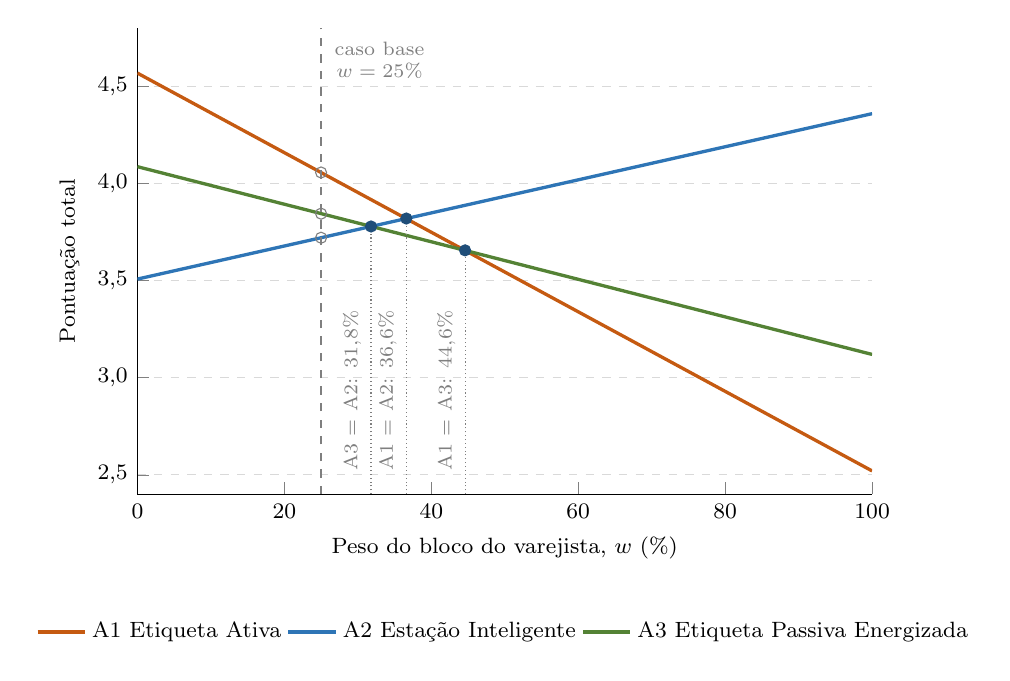
\begin{tikzpicture}
        \begin{axis}[
            r2eixo,
            width=0.9\textwidth,
            height=7.5cm,
            xmin=0, xmax=100,
            ymin=2.4, ymax=4.8,
            xtick={0,20,40,60,80,100},
            ytick={2.5,3.0,3.5,4.0,4.5},
            yticklabel style={/pgf/number format/fixed, /pgf/number format/fixed zerofill, /pgf/number format/precision=1},
            xlabel={Peso do bloco do varejista, $w$ (\%)},
            ylabel={Pontuação total},
            legend style={at={(0.5,-0.25)}, anchor=north},
            legend columns=3,
            legend cell align=left,
        ]
            \addplot[r2laranja, very thick] coordinates {(0,4.569) (100,2.520)};
            \addlegendentry{A1 Etiqueta Ativa}
            \addplot[r2azulmedio, very thick] coordinates {(0,3.508) (100,4.360)};
            \addlegendentry{A2 Estação Inteligente}
            \addplot[r2verde, very thick] coordinates {(0,4.087) (100,3.120)};
            \addlegendentry{A3 Etiqueta Passiva Energizada}
            \draw[r2cinza, dashed, thick] (axis cs:25,2.4) -- (axis cs:25,4.8);
            \node[r2rotulo, anchor=north west] at (axis cs:25.5,4.78) {caso base\\$w = 25\%$};
            \addplot[only marks, mark=o, mark size=2pt, r2cinza, forget plot] coordinates {(25,4.057) (25,3.721) (25,3.845)};
            \draw[r2cinza, densely dotted] (axis cs:31.8,2.4) -- (axis cs:31.8,3.779);
            \draw[r2cinza, densely dotted] (axis cs:36.6,2.4) -- (axis cs:36.6,3.820);
            \draw[r2cinza, densely dotted] (axis cs:44.6,2.4) -- (axis cs:44.6,3.656);
            \addplot[only marks, mark=*, mark size=2pt, r2azul, forget plot] coordinates {(31.8,3.779) (36.6,3.820) (44.6,3.656)};
            \node[r2rotulo, rotate=90, anchor=south west] at (axis cs:31.8,2.47) {A3 = A2: 31,8\%};
            \node[r2rotulo, rotate=90, anchor=south west] at (axis cs:36.6,2.47) {A1 = A2: 36,6\%};
            \node[r2rotulo, rotate=90, anchor=south west] at (axis cs:44.6,2.47) {A1 = A3: 44,6\%};
        \end{axis}
    \end{tikzpicture}
    \source{Elaborado pelos autores (2026).}
\end{figure}

No caso base, com $w = 25\%$, a ordem é A1, A3 e A2. A A2 passa à frente da A3 quando o bloco do varejista pesa 31,8\% ou mais, e passa à frente da A1 a partir de 36,6\%, ponto em que as duas empatam com cerca de 3,82 pontos; a A3 só alcançaria a A1 com 44,6\%. Entre 31,8\% e 36,6\%, a A1 continua na frente, e a A2 sobe para o segundo lugar. A folga da escolha é, portanto, de 11,6 pontos percentuais sobre o peso adotado: se a Riachuelo atribuir ao custo de implantação, à operação e à maturidade um peso de cerca de um terço da decisão, a A1 ainda vence; se esse peso chegar a 36,6\%, a Estação Inteligente passa a ser a melhor alternativa. A equipe concluiu que a escolha é robusta a variações moderadas dos pesos e sensível a uma mudança de perspectiva, do cliente para o comprador, o que torna a validação desses pesos com a Riachuelo uma tarefa do Relatório 3.

\subsection{Concepção escolhida}

A equipe escolheu a A1 Etiqueta Ativa, a única alternativa que cumpre R06 e R03 no nível máximo sem exigir um ponto fixo no fluxo principal. A escolha depende de dois testes. O primeiro é validar com a Riachuelo os pesos do bloco do varejista, porque, se esse bloco pesar 36,6\% ou mais na decisão, a A2 vence. O segundo é o marco de go/no-go do Core Bluetooth num App Clip real, previsto para o protótipo do Relatório 3; se o recurso não funcionar, a Compra Rápida no iPhone perde a liberação na própria peça e passa a depender do Liberador de Balcão.

A A2 Estação Inteligente ficou registrada como concepção de reserva e como etapa intermediária de implantação: uma loja pode começar pela estação, com R\$~28.877 por loja, e migrar para a etiqueta ativa quando a economia se confirmar, aproveitando a Plataforma Tag\&Go e os canais do cliente, que são comuns às duas. A A3 ficou como evolução futura sem bateria, caso o NFC do iPhone venha a permitir a colheita de energia pelo App Clip. A diferença de custo entre a A1 (R\$~414.458 por loja) e a A2 é o principal argumento contra a escolha, e, na Seção~\ref{sec:r2-valor}, a equipe avaliou em que condições o benefício para a Riachuelo cobre esse custo. A arquitetura da A1, com seus subsistemas, componentes e interfaces, e o desenho reformulado da etiqueta estão na Seção~\ref{sec:r2-arquitetura}.

\newpage% =============================================================================
% Relatorio 2, Secao 7: reformulacao dos desenhos e arquitetura do produto
% (item E do roteiro, parte 2). Fonte unica: biblia do R2 (secoes 4.4, 4.5,
% 4.7 e 10; figuras FIG11 a FIG16; tabelas TAB15, TAB16 e TAB17).
% Nao repete matriz de decisao, precos nem receita (ver Secoes 4 e 6).
% Figuras em TikZ e pgfplots com os estilos de r2/pacotes.tex.
% =============================================================================

\section{REFORMULAÇÃO DOS DESENHOS E ARQUITETURA DO PRODUTO}
\label{sec:r2-arquitetura}

A concepção A1 Etiqueta Ativa, escolhida na Seção~\ref{sec:r2-concepcao}, foi desdobrada em quatro resultados do projeto conceitual: a arquitetura do sistema, com seus subsistemas, componentes e interfaces; o desenho reformulado da etiqueta; os fluxos das duas jornadas de uso; e o ciclo logístico que devolve a etiqueta à origem. A equipe seguiu o roteiro da disciplina \cite{zancul2026conceitual}, baseado em \citeonline{rozenfeld2006gestao}, que pede, na fase conceitual, a identificação dos sistemas, subsistemas e componentes (SSCs) e a definição de como eles se fixam, se posicionam e trocam energia, material e sinal. Formas definitivas, materiais e a lista de materiais detalhada ficam para o Relatório 3. As funções citadas pelos códigos F1 a F31 são as da Tabela~\ref{tab:r2-funcoes}, e as especificações-meta R, E e S são as da Tabela~\ref{tab:r2-especificacoes}.

\subsection{Arquitetura modular e subsistemas}

A equipe adotou uma arquitetura modular que combina três tipos de modularidade descritos por \citeonline{rozenfeld2006gestao}. A etiqueta e a Plataforma Tag\&Go são compartilhadas pelos dois caminhos de uso, o que corresponde à modularidade de compartilhamento de componentes: a mesma etiqueta, com o mesmo firmware, atende à Compra Rápida e à Jornada Completa. Os canais do cliente, por sua vez, funcionam como módulos de interface intercambiáveis, que adaptam o sistema à variedade de aparelhos e de perfis de uso, do App Clip no iPhone ao passe do Ria Club na carteira do celular. Os serviços da Plataforma, por fim, ligam-se por um barramento de eventos, de modo que um serviço novo, ou a integração com o estoque de outro varejista, pode ser acoplado sem alterar os demais. Essa última escolha tem consequência comercial, já que a expansão para outras redes do segmento, discutida na Seção~\ref{sec:r2-comercializacao}, exigirá trocar apenas os módulos de integração.

O sistema foi dividido em cinco subsistemas, reunidos na Tabela~\ref{tab:r2-ssc} com seus componentes e as funções que cada um realiza. A etiqueta Tag\&Go (SS1) concentra as funções físicas que acompanham a peça: reter, identificar, validar a autorização, desfazer a retenção, armazenar energia, confirmar a intenção do cliente, indicar o estado da liberação e sinalizar a saída indevida. A Plataforma Tag\&Go (SS2) reúne seis serviços em nuvem e realiza as funções de informação, do processamento do pagamento ao rastreamento da frota, além de todas as funções da Jornada Completa. Os canais do cliente (SS3) formam a camada que o consumidor vê e toca. A infraestrutura de loja (SS4) e o ciclo logístico (SS5) realizam as funções que surgiram quando a etiqueta deixou de ser consumível e passou a ser um ativo retornável: recolher, registrar a devolução, transportar, inspecionar, recarregar, associar e fixar a etiqueta em uma nova peça e destinar as reprovadas.

\begin{table}[htbp]
    \centering
    \caption{Subsistemas, componentes e funções realizadas}
    \label{tab:r2-ssc}
    \scriptsize
    \renewcommand{\arraystretch}{1.25}
    \begin{tabularx}{\textwidth}{@{}
        >{\RaggedRight\arraybackslash}p{2.3cm}
        >{\RaggedRight\arraybackslash}X
        >{\RaggedRight\arraybackslash}p{2.6cm}@{}}
        \toprule
        \textbf{SSC} & \textbf{Componentes} & \textbf{Funções realizadas} \\
        \midrule
        SS1 Etiqueta Tag\&Go
            & C1.1 carcaça superior (janela do QR, LED, botão, furo do buzzer e 3 contatos de serviço); C1.2 carcaça inferior (furo do pino, sede da garra, parafusos de segurança); C1.3 garra (3 esferas, copo cônico, carretel não ferromagnético, mola e sensor de presença do pino); C1.4 pino; C1.5 atuador (micromotor com redução, came, cursor com rampa e mola de retorno); C1.6 placa única (módulo ESP32-C3-MINI-1, CI de carga e driver do motor); C1.7 célula LiPo de 150\,mAh com proteção; C1.8 interface (LED RGB, botão e buzzer piezo); C1.9 identificação (QR de 28\,mm impresso e NFC NTAG213 sobre manta de ferrite); C1.10 elemento EAS (AM ou RF, conforme o pórtico da loja)
            & F1, F2, F5, F6, F7, F10, F11, F12 \\
        \addlinespace
        SS2 Plataforma Tag\&Go
            & C2.1 Itens e Carrinho; C2.2 Pagamento; C2.3 Autorização (com HSM); C2.4 Ciclo da Etiqueta (estados, frota e alertas); C2.5 Jornada (perfil, localização N1, disponibilidade, recomendação, sustentabilidade e consentimento); C2.6 Integrações (estoque RFID e OMS, PDV e NFC-e, Ria Club, e-commerce)
            & F2, F3, F4, F13, F14, F18, F21, F23, F25 a F31 \\
        \addlinespace
        SS3 Canais do cliente
            & C3.1 App Clip Tag\&Go; C3.2 Página de Compra Rápida; C3.3 módulo Tag\&Go do app Riachuelo; C3.4 passe do Ria Club
            & F3, F9, F11, F15, F25 a F31 \\
        \addlinespace
        SS4 Infraestrutura de loja
            & C4.1 Coletor de Etiquetas (caixa trancada, boca antirretorno em cor contrastante entre 0,40 e 1,20\,m do piso, leitor BLE, contador óptico, sinal de recebida, capacidade de cerca de 150 etiquetas); C4.2 Liberador de Balcão (encaixe com 3 pinos de mola sobre os contatos da face superior, 5\,V, dados por UART, ligação ao PDV e à Plataforma; um por caixa e um no Ponto de Apoio); C4.3 Ponto de Apoio (balcão com funcionário, painel de etiquetas liberadas e não recolhidas, QR do Wi-Fi de convidados)
            & F8 (fonte externa), F15, F16, F17, F18 \\
        \addlinespace
        SS5 Ciclo logístico
            & C5.1 Malote de Retorno (caixa plástica rígida e retornável, divisórias antiestáticas, lacre numerado e identificação de baterias de lítio instaladas em equipamento); C5.2 Bancada de Inspeção (teste de botão, LED, buzzer, BLE, motor, retenção por amostragem, célula e firmware; limpeza; triagem); C5.3 Bandeja de Recarga (20 posições com pinos sobre a face superior; cerca de 2\,h por carga); C5.4 Estação de Cadastro (leitor UHF do EPC, contatos para o \texttt{tag\_id}, aplicação do pino e registro da associação)
            & F8, F19, F20, F21, F22, F24 \\
        \bottomrule
    \end{tabularx}
    \source{Elaborado pelos autores (2026).}
\end{table}

A fronteira entre a etiqueta e a Plataforma seguiu uma regra de projeto: a etiqueta guarda apenas o necessário para decidir se abre, isto é, a própria chave, o nonce vigente e a condição da trava, enquanto preço, estado oficial, histórico e regras comerciais ficam na Plataforma. Com isso, a etiqueta permanece simples, e uma mudança de regra de negócio não exige regravar o firmware da frota. Os elementos externos ao Tag\&Go foram mantidos fora da fronteira do produto porque a Riachuelo já os opera: o PSP e as carteiras digitais (Apple Pay, Google Pay e Pix), o estoque RFID implantado com a Mozaiko \cite{tiinside2022riachuelo}, o OMS da Manhattan \cite{manhattan2026riachuelo}, o PDV e o emissor de NFC-e, os pórticos EAS e RFID das lojas, o app Riachuelo, o Ria Club e o e-commerce. O sistema se apoia neles por meio de interfaces definidas, sem substituí-los.

\subsection{Interfaces entre os subsistemas}

A matriz de interfaces (Tabela~\ref{tab:r2-interfaces}) registra 18 interfaces, classificadas pelo tipo de fluxo, energia, material ou sinal, como na caixa-preta da Seção~\ref{sec:r2-funcional}. As cinco primeiras, I1 a I5, são internas à etiqueta e descrevem a cadeia mecânica e elétrica da liberação: o pino retido pela garra, o cursor com rampa que ergue o carretel, a célula que alimenta a placa, a placa que aciona o micromotor e a interface com o cliente. As interfaces I6 e I7 ligam a etiqueta ao celular, a primeira por leitura óptica ou por aproximação (QR e NFC) e a segunda por rádio (BLE). As interfaces I8 a I12 são digitais e ligam os canais à Plataforma e a Plataforma aos sistemas da Riachuelo e do PSP. As interfaces I13 a I16 acontecem na loja, e I17 e I18, no ciclo logístico. A Figura~\ref{fig:r2-arquitetura} representa a mesma estrutura em forma de diagrama, com cada interface desenhada segundo o seu tipo.

Três interfaces concentram os riscos técnicos do conceito. A interface I7, BLE sem pareamento com filtro pelo \texttt{tag\_id}, depende de o App Clip poder usar Core Bluetooth no iPhone, o que a equipe deduziu da documentação da Apple sem confirmação explícita \cite{apple2026appclipfuncoes, apple2020forumble}, e do Web Bluetooth, que no Android existe no Chrome e no Samsung Internet \cite{chrome2026webbluetooth}; por isso, ela será o primeiro marco de go/no-go do protótipo. A interface I13, formada por três contatos na face superior que levam 5\,V e dados seriais, viabiliza a liberação assistida para qualquer falha da etiqueta ou do celular e, com ela, o carretel não ferromagnético. A interface I10, com a baixa do EPC como vendido no estoque RFID em até 5\,s após a confirmação do pagamento (S07), fecha a malha antifraude com o pórtico RFID, que alarma quando sai da loja uma peça cujo EPC não foi vendido. Há ainda um requisito elétrico em I3: a placa precisa de um caminho de energia que a deixe ligar pelos contatos mesmo com a célula descarregada, sem o qual o Liberador de Balcão não conseguiria abrir uma etiqueta sem carga.

\begingroup
\captionsetup{font=normalsize}
\scriptsize
\setlength{\tabcolsep}{4pt}
\renewcommand{\arraystretch}{1.25}
\begin{longtable}{@{}
    >{\RaggedRight\arraybackslash}p{0.8cm}
    >{\RaggedRight\arraybackslash}p{4.2cm}
    >{\RaggedRight\arraybackslash}p{1.0cm}
    >{\RaggedRight\arraybackslash}p{9.0cm}@{}}
\caption{Matriz de interfaces} \label{tab:r2-interfaces} \\
\toprule
\textbf{Código} & \textbf{Entre} & \textbf{Tipo} & \textbf{Descrição e especificação} \\
\midrule
\endfirsthead
\multicolumn{4}{c}{Tabela~\ref{tab:r2-interfaces} (continuação)} \\
\toprule
\textbf{Código} & \textbf{Entre} & \textbf{Tipo} & \textbf{Descrição e especificação} \\
\midrule
\endhead
\midrule
\multicolumn{4}{r}{\textit{continua na próxima página}} \\
\endfoot
\bottomrule
\multicolumn{4}{c}{Fonte: Elaborado pelos autores (2026). Tipo: E, energia; M, material; S, sinal.} \\
\endlastfoot
I1 & C1.4 pino $\leftrightarrow$ C1.3 garra & M & haste de $\varnothing$\,2\,mm retida por 3 esferas; tecido de 1\,mm prensado entre a face inferior e o disco do pino; E02 $\geq$ 120\,N \\
I2 & C1.5 cursor $\rightarrow$ C1.3 carretel & E & força e curso: a rampa converte o avanço horizontal do cursor em 1,2\,mm verticais do carretel; E04 $\geq$ 3 \\
I3 & C1.7 célula $\leftrightarrow$ C1.6 placa & E & 3,7\,V; proteção de subtensão e de sobretensão; caminho de energia que deixa a placa ligar pelos contatos mesmo com a célula descarregada \\
I4 & C1.6 placa $\leftrightarrow$ C1.5 atuador & E + S & acionamento do micromotor (cerca de 150\,mA por 0,6\,s); sensor de fim de curso \\
I5 & C1.6 placa $\leftrightarrow$ C1.8 interface & S & botão (acordar e confirmar), LED RGB e buzzer (E08) \\
I6 & C1.9 identificação $\leftrightarrow$ SS3 canais & S & leitura óptica (QR) e NFC de 13,56\,MHz com a URL do \texttt{tag\_id}; E09 \\
I7 & C1.6 placa $\leftrightarrow$ SS3 canais & S & BLE GATT sem pareamento: nonce, token e estado; filtro pelo \texttt{tag\_id} \\
I8 & SS3 canais $\leftrightarrow$ SS2 Plataforma & S & HTTPS: carrinho, pagamento, pedido de token e status da devolução \\
I9 & SS2 $\leftrightarrow$ PSP e carteiras & S & tokens de pagamento, confirmação e webhook do Pix \\
I10 & SS2 $\leftrightarrow$ estoque RFID e OMS & S & preço pelo EPC; disponibilidade (leitura com idade $\leq$ 24\,h); baixa como vendido (S07); pedido on-line do tamanho ausente \\
I11 & SS2 $\leftrightarrow$ PDV e NFC-e & S & compra no caixa, emissão fiscal e localização da compra pelo funcionário \\
I12 & SS2 $\leftrightarrow$ app Riachuelo e Ria Club & S & perfil, cashback liberado após a devolução da etiqueta, recomendação \\
I13 & C4.2 Liberador $\leftrightarrow$ etiqueta (contatos da face superior) & E + S & 5\,V e UART nos 3 contatos; energiza a etiqueta descarregada e entrega o token \\
I14 & C4.2 Liberador $\leftrightarrow$ SS2 e PDV & S & pedido autenticado de token depois do pagamento no PDV ou da localização da compra (S09) \\
I15 & C4.1 Coletor $\leftrightarrow$ etiqueta & M + S & recebe a etiqueta pela boca antirretorno; lê o \texttt{tag\_id} por BLE no estado DESTRAVADA; comunica RECOLHIDA à Plataforma \\
I16 & C1.10 elemento EAS $\leftrightarrow$ pórtico EAS & S & campo AM de 58\,kHz ou RF de 8,2\,MHz; alarme se a etiqueta liberada sair da loja (M1) \\
I17 & SS5 $\leftrightarrow$ etiqueta & M + E & transporte no Malote de Retorno; recarga pelos contatos na Bandeja de Recarga; testes na Bancada de Inspeção \\
I18 & C5.4 Estação de Cadastro $\leftrightarrow$ etiqueta e peça & M + S & fixa o pino na peça; lê o EPC por UHF e o \texttt{tag\_id} pelos contatos; grava a associação e o estado TRAVADA \\
\end{longtable}
\endgroup

\begin{landscape}
\begin{figure}[htbp]
    \centering
    \caption{Arquitetura do produto: subsistemas, componentes e interfaces}
    \label{fig:r2-arquitetura}
    \resizebox{\linewidth}{!}{%
    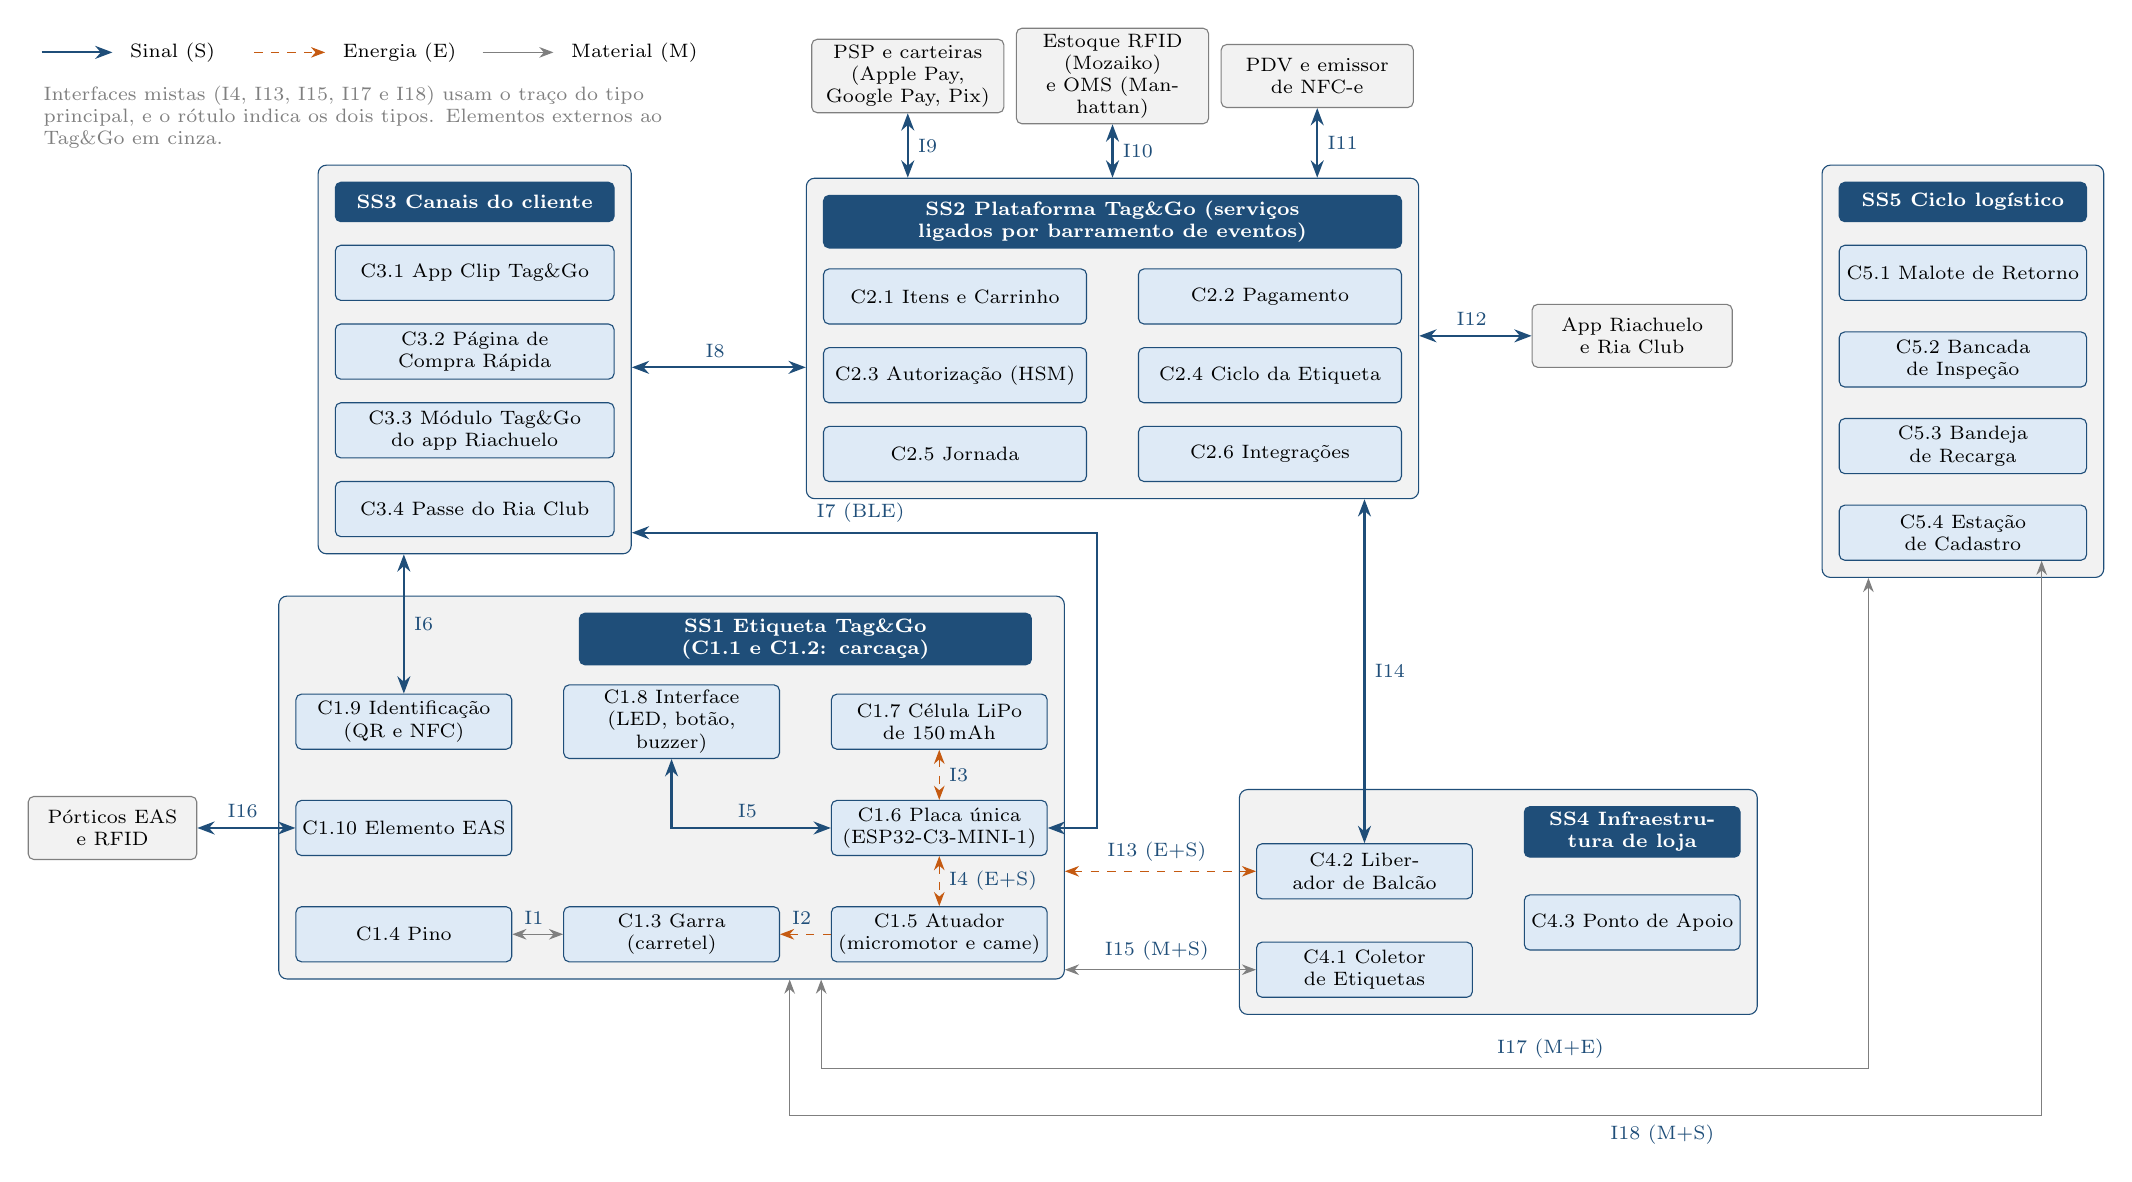
\begin{tikzpicture}[font=\scriptsize]
        % ---------------- SS3 canais do cliente ----------------
        \node[r2blocoescuro, font=\scriptsize\bfseries, text width=3.4cm, minimum height=5mm, inner sep=2pt] (t3) at (2.3,10.1) {SS3 Canais do cliente};
        \node[r2bloco, font=\scriptsize, text width=3.4cm, minimum height=7mm, inner sep=2pt] (c31) at (2.3,9.2) {C3.1 App Clip Tag\&Go};
        \node[r2bloco, font=\scriptsize, text width=3.4cm, minimum height=7mm, inner sep=2pt] (c32) at (2.3,8.2) {C3.2 Página de Compra Rápida};
        \node[r2bloco, font=\scriptsize, text width=3.4cm, minimum height=7mm, inner sep=2pt] (c33) at (2.3,7.2) {C3.3 Módulo Tag\&Go do app Riachuelo};
        \node[r2bloco, font=\scriptsize, text width=3.4cm, minimum height=7mm, inner sep=2pt] (c34) at (2.3,6.2) {C3.4 Passe do Ria Club};
        % ---------------- SS2 Plataforma ----------------
        \node[r2blocoescuro, font=\scriptsize\bfseries, text width=7.2cm, minimum height=5mm, inner sep=2pt] (t2) at (10.4,9.85) {SS2 Plataforma Tag\&Go (serviços ligados por barramento de eventos)};
        \node[r2bloco, font=\scriptsize, text width=3.2cm, minimum height=7mm, inner sep=2pt] (c21) at (8.4,8.9) {C2.1 Itens e Carrinho};
        \node[r2bloco, font=\scriptsize, text width=3.2cm, minimum height=7mm, inner sep=2pt] (c22) at (12.4,8.9) {C2.2 Pagamento};
        \node[r2bloco, font=\scriptsize, text width=3.2cm, minimum height=7mm, inner sep=2pt] (c23) at (8.4,7.9) {C2.3 Autorização (HSM)};
        \node[r2bloco, font=\scriptsize, text width=3.2cm, minimum height=7mm, inner sep=2pt] (c24) at (12.4,7.9) {C2.4 Ciclo da Etiqueta};
        \node[r2bloco, font=\scriptsize, text width=3.2cm, minimum height=7mm, inner sep=2pt] (c25) at (8.4,6.9) {C2.5 Jornada};
        \node[r2bloco, font=\scriptsize, text width=3.2cm, minimum height=7mm, inner sep=2pt] (c26) at (12.4,6.9) {C2.6 Integrações};
        % ---------------- SS1 Etiqueta ----------------
        \node[r2blocoescuro, font=\scriptsize\bfseries, text width=5.6cm, minimum height=5mm, inner sep=2pt] (t1) at (6.5,4.55) {SS1 Etiqueta Tag\&Go (C1.1 e C1.2: carcaça)};
        \node[r2bloco, font=\scriptsize, text width=2.6cm, minimum height=7mm, inner sep=2pt] (c19) at (1.4,3.5) {C1.9 Identificação\\ (QR e NFC)};
        \node[r2bloco, font=\scriptsize, text width=2.6cm, minimum height=7mm, inner sep=2pt] (c18) at (4.8,3.5) {C1.8 Interface\\ (LED, botão, buzzer)};
        \node[r2bloco, font=\scriptsize, text width=2.6cm, minimum height=7mm, inner sep=2pt] (c17) at (8.2,3.5) {C1.7 Célula LiPo\\ de 150\,mAh};
        \node[r2bloco, font=\scriptsize, text width=2.6cm, minimum height=7mm, inner sep=2pt] (c110) at (1.4,2.15) {C1.10 Elemento EAS};
        \node[r2bloco, font=\scriptsize, text width=2.6cm, minimum height=7mm, inner sep=2pt] (c16) at (8.2,2.15) {C1.6 Placa única\\ (ESP32-C3-MINI-1)};
        \node[r2bloco, font=\scriptsize, text width=2.6cm, minimum height=7mm, inner sep=2pt] (c14) at (1.4,0.8) {C1.4 Pino};
        \node[r2bloco, font=\scriptsize, text width=2.6cm, minimum height=7mm, inner sep=2pt] (c13) at (4.8,0.8) {C1.3 Garra\\ (carretel)};
        \node[r2bloco, font=\scriptsize, text width=2.6cm, minimum height=7mm, inner sep=2pt] (c15) at (8.2,0.8) {C1.5 Atuador\\ (micromotor e came)};
        % ---------------- SS4 Infraestrutura de loja ----------------
        \node[r2blocoescuro, font=\scriptsize\bfseries, text width=2.6cm, minimum height=5mm, inner sep=2pt] (t4) at (17.0,2.1) {SS4 Infraestrutura de loja};
        \node[r2bloco, font=\scriptsize, text width=2.6cm, minimum height=7mm, inner sep=2pt] (c42) at (13.6,1.6) {C4.2 Liberador de Balcão};
        \node[r2bloco, font=\scriptsize, text width=2.6cm, minimum height=7mm, inner sep=2pt] (c41) at (13.6,0.35) {C4.1 Coletor de Etiquetas};
        \node[r2bloco, font=\scriptsize, text width=2.6cm, minimum height=7mm, inner sep=2pt] (c43) at (17.0,0.95) {C4.3 Ponto de Apoio};
        % ---------------- SS5 Ciclo logistico ----------------
        \node[r2blocoescuro, font=\scriptsize\bfseries, text width=3.0cm, minimum height=5mm, inner sep=2pt] (t5) at (21.2,10.1) {SS5 Ciclo logístico};
        \node[r2bloco, font=\scriptsize, text width=3.0cm, minimum height=7mm, inner sep=2pt] (c51) at (21.2,9.2) {C5.1 Malote de Retorno};
        \node[r2bloco, font=\scriptsize, text width=3.0cm, minimum height=7mm, inner sep=2pt] (c52) at (21.2,8.1) {C5.2 Bancada de Inspeção};
        \node[r2bloco, font=\scriptsize, text width=3.0cm, minimum height=7mm, inner sep=2pt] (c53) at (21.2,7.0) {C5.3 Bandeja de Recarga};
        \node[r2bloco, font=\scriptsize, text width=3.0cm, minimum height=7mm, inner sep=2pt] (c54) at (21.2,5.9) {C5.4 Estação de Cadastro};
        % ---------------- elementos externos ----------------
        \node[r2neutro, font=\scriptsize, text width=2.3cm, inner sep=2pt] (psp) at (7.8,11.7) {PSP e carteiras\\ (Apple Pay, Google Pay, Pix)};
        \node[r2neutro, font=\scriptsize, text width=2.3cm, inner sep=2pt] (est) at (10.4,11.7) {Estoque RFID (Mozaiko)\\ e OMS (Manhattan)};
        \node[r2neutro, font=\scriptsize, text width=2.3cm, inner sep=2pt] (pdv) at (13.0,11.7) {PDV e emissor\\ de NFC-e};
        \node[r2neutro, font=\scriptsize, text width=2.4cm, inner sep=2pt] (app) at (17.0,8.4) {App Riachuelo\\ e Ria Club};
        \node[r2neutro, font=\scriptsize, text width=2.0cm, inner sep=2pt] (por) at (-2.3,2.15) {Pórticos EAS\\ e RFID};
        % ---------------- contornos dos subsistemas ----------------
        \begin{scope}[on background layer]
            \node[draw=r2azul, fill=r2cinzaclaro, rounded corners=3pt, inner sep=6pt, fit=(t3)(c31)(c32)(c33)(c34)] (ss3) {};
            \node[draw=r2azul, fill=r2cinzaclaro, rounded corners=3pt, inner sep=6pt, fit=(t2)(c21)(c22)(c23)(c24)(c25)(c26)] (ss2) {};
            \node[draw=r2azul, fill=r2cinzaclaro, rounded corners=3pt, inner sep=6pt, fit=(t1)(c19)(c18)(c17)(c110)(c16)(c14)(c13)(c15)] (ss1) {};
            \node[draw=r2azul, fill=r2cinzaclaro, rounded corners=3pt, inner sep=6pt, fit=(t4)(c41)(c42)(c43)] (ss4) {};
            \node[draw=r2azul, fill=r2cinzaclaro, rounded corners=3pt, inner sep=6pt, fit=(t5)(c51)(c52)(c53)(c54)] (ss5) {};
        \end{scope}
        % ---------------- coordenadas auxiliares ----------------
        \coordinate (y80) at (0,8.0);
        \coordinate (y59) at (0,5.9);
        \coordinate (x102) at (10.2,0);
        \coordinate (x200) at (20.0,0);
        \coordinate (x222) at (22.2,0);
        \coordinate (x67) at (6.7,0);
        \coordinate (x63) at (6.3,0);
        % ---------------- interfaces internas da etiqueta ----------------
        \draw[r2setafina, {Stealth[length=1.8mm]}-{Stealth[length=1.8mm]}] (c14.east) -- node[r2rotulo, text=r2azul, above] {I1} (c13.west);
        \draw[r2setatracejada] (c15.west) -- node[r2rotulo, text=r2azul, above] {I2} (c13.east);
        \draw[r2setatracejada, {Stealth[length=1.8mm]}-{Stealth[length=1.8mm]}] (c17.south) -- node[r2rotulo, text=r2azul, right] {I3} (c16.north);
        \draw[r2setatracejada, {Stealth[length=1.8mm]}-{Stealth[length=1.8mm]}] (c16.south) -- node[r2rotulo, text=r2azul, right] {I4 (E+S)} (c15.north);
        \draw[r2seta, {Stealth[length=2.2mm]}-{Stealth[length=2.2mm]}] (c16.west) -| node[r2rotulo, text=r2azul, pos=0.25, above] {I5} (c18.south);
        % ---------------- etiqueta e canais ----------------
        \draw[r2seta, {Stealth[length=2.2mm]}-{Stealth[length=2.2mm]}] (c19.north) -- node[r2rotulo, text=r2azul, right] {I6} (c19.north |- ss3.south);
        \draw[r2seta, {Stealth[length=2.2mm]}-{Stealth[length=2.2mm]}] (c16.east) -- (x102 |- c16.east) -- (x102 |- y59) -- node[r2rotulo, text=r2azul, above] {I7 (BLE)} (ss3.east |- y59);
        % ---------------- canais e Plataforma ----------------
        \draw[r2seta, {Stealth[length=2.2mm]}-{Stealth[length=2.2mm]}] (ss3.east |- y80) -- node[r2rotulo, text=r2azul, above] {I8} (ss2.west |- y80);
        % ---------------- Plataforma e externos ----------------
        \draw[r2seta, {Stealth[length=2.2mm]}-{Stealth[length=2.2mm]}] (psp.south) -- node[r2rotulo, text=r2azul, right] {I9} (psp.south |- ss2.north);
        \draw[r2seta, {Stealth[length=2.2mm]}-{Stealth[length=2.2mm]}] (est.south) -- node[r2rotulo, text=r2azul, right] {I10} (est.south |- ss2.north);
        \draw[r2seta, {Stealth[length=2.2mm]}-{Stealth[length=2.2mm]}] (pdv.south) -- node[r2rotulo, text=r2azul, right] {I11} (pdv.south |- ss2.north);
        \draw[r2seta, {Stealth[length=2.2mm]}-{Stealth[length=2.2mm]}] (ss2.east |- app.west) -- node[r2rotulo, text=r2azul, above] {I12} (app.west);
        % ---------------- loja ----------------
        \draw[r2setatracejada, {Stealth[length=1.8mm]}-{Stealth[length=1.8mm]}] (ss1.east |- c42.west) -- node[r2rotulo, text=r2azul, above] {I13 (E+S)} (c42.west);
        \draw[r2seta, {Stealth[length=2.2mm]}-{Stealth[length=2.2mm]}] (c42.north) -- node[r2rotulo, text=r2azul, right] {I14} (c42.north |- ss2.south);
        \draw[r2setafina, {Stealth[length=1.8mm]}-{Stealth[length=1.8mm]}] (ss1.east |- c41.west) -- node[r2rotulo, text=r2azul, above] {I15 (M+S)} (c41.west);
        \draw[r2seta, {Stealth[length=2.2mm]}-{Stealth[length=2.2mm]}] (c110.west) -- node[r2rotulo, text=r2azul, above] {I16} (por.east);
        % ---------------- ciclo logistico ----------------
        \draw[r2setafina, {Stealth[length=1.8mm]}-{Stealth[length=1.8mm]}] (x200 |- ss5.south) -- (20.0,-0.9) -- node[r2rotulo, text=r2azul, above, pos=0.3] {I17 (M+E)} (6.7,-0.9) -- (x67 |- ss1.south);
        \draw[r2setafina, {Stealth[length=1.8mm]}-{Stealth[length=1.8mm]}] (x222 |- c54.south) -- (22.2,-1.5) -- node[r2rotulo, text=r2azul, below, pos=0.3] {I18 (M+S)} (6.3,-1.5) -- (x63 |- ss1.south);
        % ---------------- legenda ----------------
        \draw[r2seta] (-3.2,12.0) -- (-2.3,12.0);
        \node[anchor=west, font=\scriptsize] at (-2.2,12.0) {Sinal (S)};
        \draw[r2setatracejada] (-0.5,12.0) -- (0.4,12.0);
        \node[anchor=west, font=\scriptsize] at (0.5,12.0) {Energia (E)};
        \draw[r2setafina] (2.4,12.0) -- (3.3,12.0);
        \node[anchor=west, font=\scriptsize] at (3.4,12.0) {Material (M)};
        \node[r2rotulo, anchor=north west, text width=8.3cm, align=left] at (-3.3,11.7) {Interfaces mistas (I4, I13, I15, I17 e I18) usam o traço do tipo principal, e o rótulo indica os dois tipos. Elementos externos ao Tag\&Go em cinza.};
    \end{tikzpicture}%
    }
    \source{Elaborado pelos autores (2026).}
\end{figure}
\end{landscape}

\subsection{Desenho reformulado da etiqueta}

A Figura~\ref{fig:r2-desenho} compara a planta apresentada no Relatório 1 com o esquema reformulado. O envelope externo foi mantido em $98 \times 82 \times 26$\,mm (E01), com o plano de partição a 13\,mm da face inferior, e o arranjo interno foi redefinido a partir das funções e dos princípios escolhidos: o mecanismo de liberação (garra, cursor com rampa, came e micromotor) ocupa o lado esquerdo, a placa única e a célula ocupam o lado direito, e o elemento EAS fica no canto superior esquerdo, afastado das partes metálicas. Na face superior, o QR ocupa a região central, agora com a antena NFC sob ele, e os três contatos de serviço ficam no canto superior direito. O corte A-A, pelo eixo da garra, mostra o tecido prensado entre a face inferior e o disco do pino e o deslocamento de 1,2\,mm do carretel que solta a haste.

\begin{figure}[htbp]
    \centering
    \caption{Desenho reformulado da etiqueta}
    \label{fig:r2-desenho}
    \begin{subfigure}{0.42\textwidth}
        \centering
        \caption{Planta do Relatório 1}
        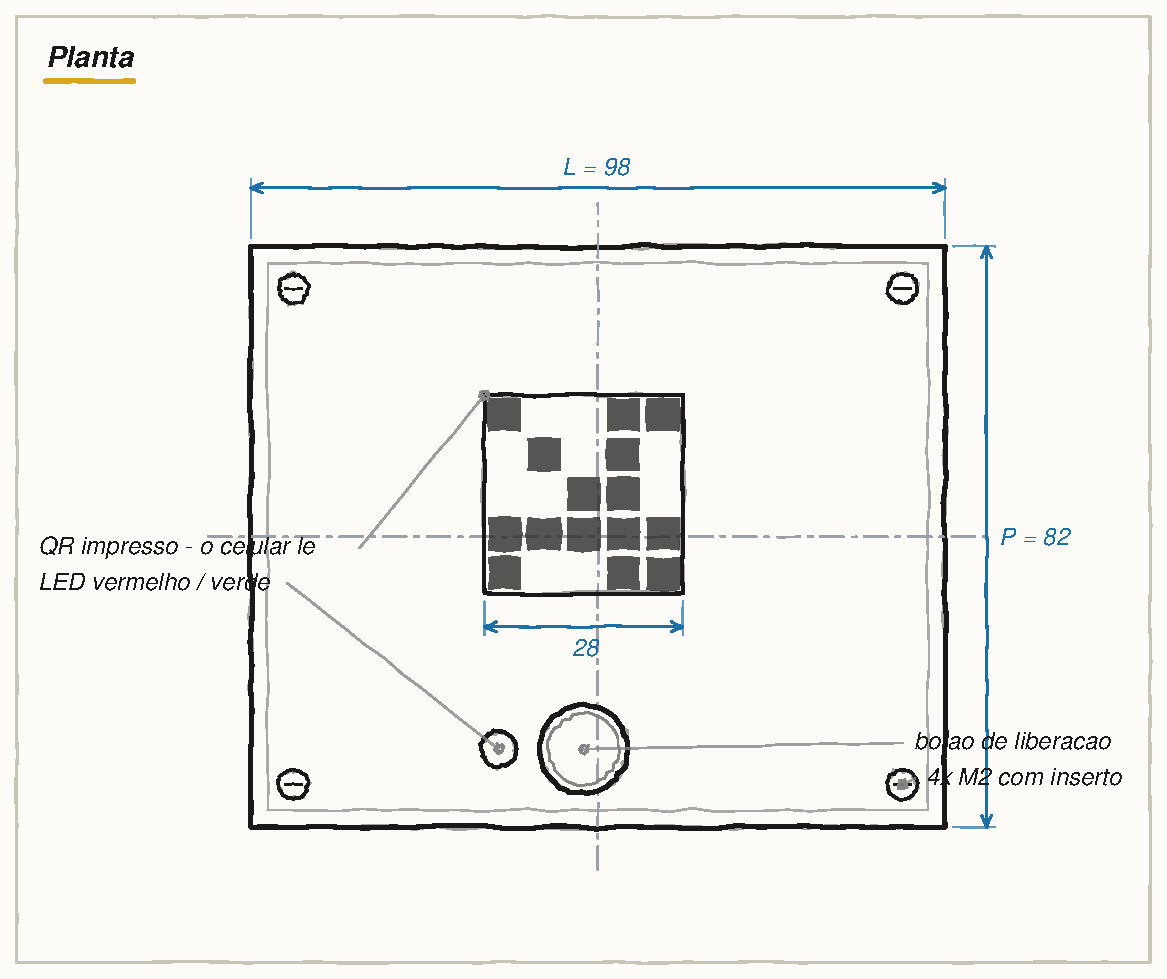
\includegraphics[width=\linewidth]{esboco/fig-planta.pdf}
    \end{subfigure}

    \medskip
    \begin{subfigure}{\textwidth}
        \centering
        \caption{Esquema reformulado: vista superior, com componentes internos tracejados, e corte A-A pela garra (cotas em mm)}
        \resizebox{0.9\linewidth}{!}{%
        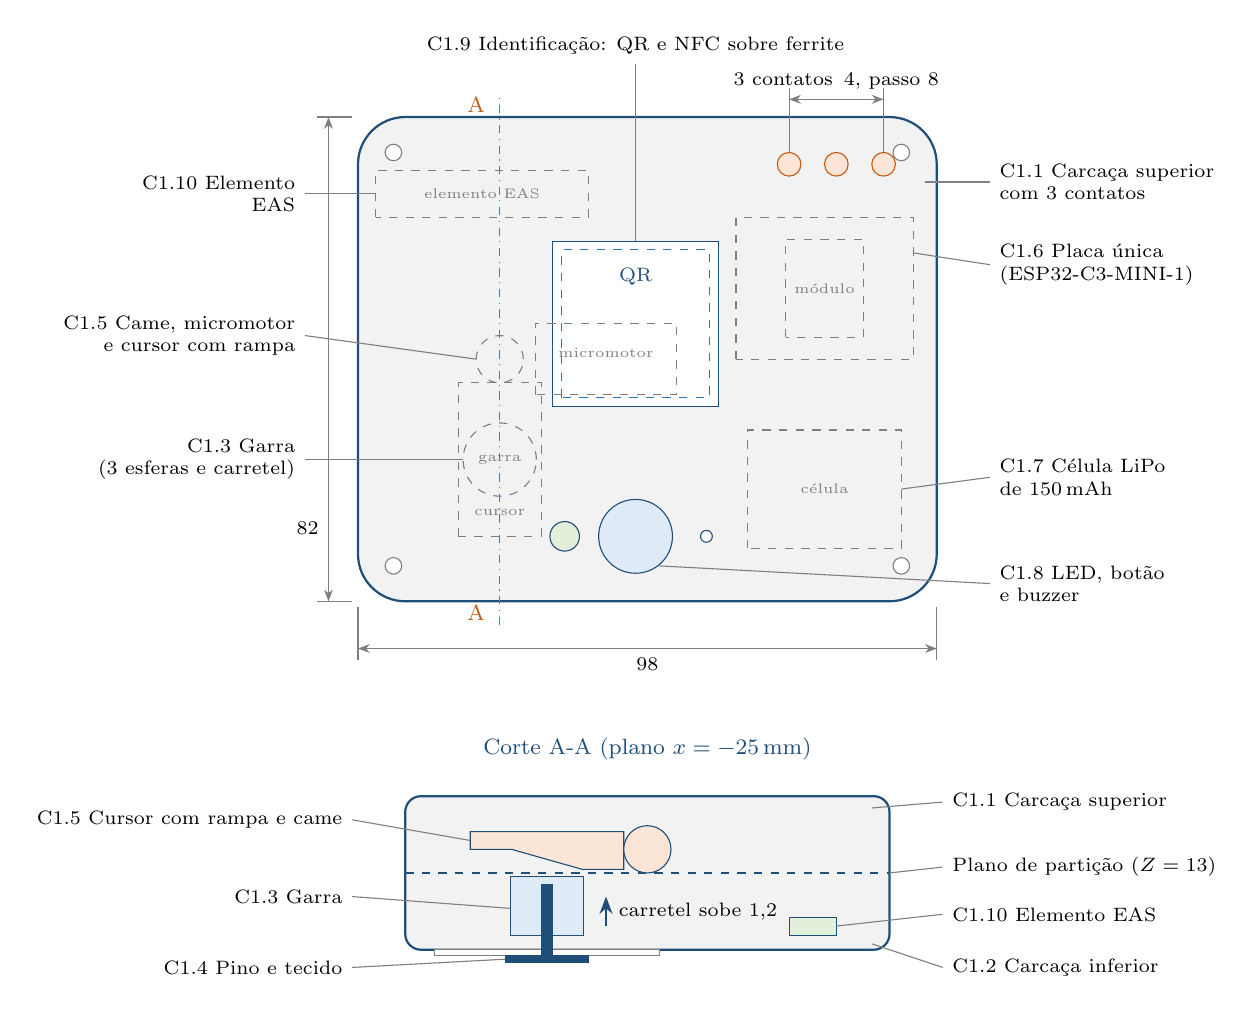
\begin{tikzpicture}[x=0.75mm, y=0.75mm, font=\scriptsize]
            % ---------------- vista superior ----------------
            \draw[thick, draw=r2azul, fill=r2cinzaclaro, rounded corners=6mm] (-49,-41) rectangle (49,41);
            \foreach \px/\py in {43/35,-43/35,43/-35,-43/-35} {\draw[draw=r2cinza, fill=white] (\px,\py) circle[radius=1.4];}
            % QR e NFC com ferrite
            \draw[draw=r2azul, fill=white] (-16,-8) rectangle (12,20);
            \draw[draw=r2azulmedio, dashed] (-14.5,-6.5) rectangle (10.5,18.5);
            \node[text=r2azul] at (-2,14) {QR};
            % LED, botao e buzzer
            \draw[draw=r2azul, fill=r2verdeclaro] (-14,-30) circle[radius=2.5];
            \draw[draw=r2azul, fill=r2azulclaro] (-2,-30) circle[radius=6.25];
            \draw[draw=r2azul, fill=white] (10,-30) circle[radius=1];
            % contatos de servico
            \foreach \cx in {24,32,40} {\draw[draw=r2laranja, fill=r2laranjaclaro] (\cx,33) circle[radius=2];}
            % componentes internos (tracejados)
            \draw[r2cinza, dashed] (-25,-17) circle[radius=6.2];
            \draw[r2cinza, dashed] (-32,-30) rectangle (-18,-4);
            \draw[r2cinza, dashed] (-25,0) circle[radius=4];
            \draw[r2cinza, dashed] (-19,-6) rectangle (5,6);
            \draw[r2cinza, dashed] (15,0) rectangle (45,24);
            \draw[r2cinza, dashed] (23.4,3.7) rectangle (36.6,20.3);
            \draw[r2cinza, dashed] (17,-32) rectangle (43,-12);
            \draw[r2cinza, dashed] (-46,24) rectangle (-10,32);
            \node[font=\tiny, text=r2cinza] at (-7,1) {micromotor};
            \node[font=\tiny, text=r2cinza] at (30,12) {módulo};
            \node[font=\tiny, text=r2cinza] at (30,-22) {célula};
            \node[font=\tiny, text=r2cinza] at (-28,28) {elemento EAS};
            \node[font=\tiny, text=r2cinza] at (-25,-17) {garra};
            \node[font=\tiny, text=r2cinza] at (-25,-26) {cursor};
            % linha de corte A-A
            \draw[r2laranja, dash dot] (-25,-45) -- (-25,45);
            \node[text=r2laranja, font=\footnotesize] at (-29,43) {A};
            \node[text=r2laranja, font=\footnotesize] at (-29,-43) {A};
            % cotas
            \draw[r2cinza] (-49,-42) -- (-49,-51);
            \draw[r2cinza] (49,-42) -- (49,-51);
            \draw[r2cinza, {Stealth[length=1.5mm]}-{Stealth[length=1.5mm]}] (-49,-49) -- node[below, text=black] {98} (49,-49);
            \draw[r2cinza] (-50,41) -- (-56,41);
            \draw[r2cinza] (-50,-41) -- (-56,-41);
            \draw[r2cinza, {Stealth[length=1.5mm]}-{Stealth[length=1.5mm]}] (-54,-41) -- node[pos=0.15, left, text=black] {82} (-54,41);
            \draw[r2cinza] (24,35) -- (24,46);
            \draw[r2cinza] (40,35) -- (40,46);
            \draw[r2cinza, {Stealth[length=1.5mm]}-{Stealth[length=1.5mm]}] (24,44) -- node[above, text=black] {3 contatos $\varnothing$\,4, passo 8} (40,44);
            % chamadas da vista superior
            \draw[r2cinza] (-2,20) -- (-2,50) node[anchor=south, text=black] {C1.9 Identificação: QR e NFC sobre ferrite};
            \draw[r2cinza] (47,30) -- (58,30) node[anchor=west, text=black, align=left] {C1.1 Carcaça superior\\ com 3 contatos};
            \draw[r2cinza] (45,18) -- (58,16) node[anchor=west, text=black, align=left] {C1.6 Placa única\\ (ESP32-C3-MINI-1)};
            \draw[r2cinza] (43,-22) -- (58,-20) node[anchor=west, text=black, align=left] {C1.7 Célula LiPo\\ de 150\,mAh};
            \draw[r2cinza] (2,-35) -- (58,-38) node[anchor=west, text=black, align=left] {C1.8 LED, botão\\ e buzzer};
            \draw[r2cinza] (-46,28) -- (-58,28) node[anchor=east, text=black, align=right] {C1.10 Elemento\\ EAS};
            \draw[r2cinza] (-29,0) -- (-58,4) node[anchor=east, text=black, align=right] {C1.5 Came, micromotor\\ e cursor com rampa};
            \draw[r2cinza] (-31.2,-17) -- (-58,-17) node[anchor=east, text=black, align=right] {C1.3 Garra\\ (3 esferas e carretel)};
            % ---------------- corte A-A ----------------
            \node[font=\footnotesize, text=r2azul] at (0,-66) {Corte A-A (plano $x = -25$\,mm)};
            \draw[thick, draw=r2azul, fill=r2cinzaclaro, rounded corners=2mm] (-41,-100) rectangle (41,-74);
            \draw[r2azul, dashed] (-41,-87) -- (41,-87);
            \draw[draw=r2azul, fill=r2azulclaro] (-23.2,-97.6) rectangle (-10.8,-87.6);
            \draw[draw=r2azul, fill=r2laranjaclaro] (-30,-80) -- (-4,-80) -- (-4,-86.4) -- (-11,-86.4) -- (-23,-83) -- (-30,-83) -- cycle;
            \draw[draw=r2azul, fill=r2laranjaclaro] (0,-83) circle[radius=4];
            \draw[draw=r2cinza, fill=white] (-36,-101) rectangle (2,-100);
            \draw[draw=r2azul, fill=r2azul] (-18,-101) rectangle (-16,-89);
            \draw[draw=r2azul, fill=r2azul] (-24,-102.2) rectangle (-10,-101);
            \draw[draw=r2azul, fill=r2verdeclaro] (24,-97.6) rectangle (32,-94.5);
            \draw[r2seta] (-7,-96) -- (-7,-91);
            \node[anchor=west] at (-6.5,-93.5) {carretel sobe 1,2};
            % chamadas do corte
            \draw[r2cinza] (-30,-81.5) -- (-50,-78) node[anchor=east, text=black] {C1.5 Cursor com rampa e came};
            \draw[r2cinza] (-23.2,-93) -- (-50,-91) node[anchor=east, text=black] {C1.3 Garra};
            \draw[r2cinza] (-24,-101.6) -- (-50,-103) node[anchor=east, text=black] {C1.4 Pino e tecido};
            \draw[r2cinza] (38,-76) -- (50,-75) node[anchor=west, text=black] {C1.1 Carcaça superior};
            \draw[r2cinza] (41,-87) -- (50,-86) node[anchor=west, text=black] {Plano de partição ($Z = 13$)};
            \draw[r2cinza] (32,-96) -- (50,-94) node[anchor=west, text=black] {C1.10 Elemento EAS};
            \draw[r2cinza] (38,-99) -- (50,-103) node[anchor=west, text=black] {C1.2 Carcaça inferior};
        \end{tikzpicture}%
        }
    \end{subfigure}
    \source{Elaborado pelos autores (2026).}
\end{figure}

As mudanças em relação ao Relatório 1 estão na Tabela~\ref{tab:r2-mudancas}, cada uma com o seu motivo. A mais visível é a transferência dos contatos de recarga da face inferior para a face superior. Nos estudos anteriores da equipe, verificou-se que a face inferior fica encostada no tecido e que os pinos de um equipamento de recarga não a alcançam com a peça presa. Com três contatos na face superior, para energia, terra e dados, a mesma interface passa a servir à recarga na Bandeja de Recarga, ao cadastro na Estação de Cadastro e à liberação assistida no Liberador de Balcão.

A troca do servo pelo micromotor com redução e came preservou o cursor com rampa, baixou o perfil do conjunto e reduziu o custo do grupo de atuação na meta de \textit{design to cost} de R\$~32,30 para R\$~9,20 (Tabela~\ref{tab:r2-bom}). Nos estudos anteriores da equipe, o came acionado por servo deu margem de força de 30,6 vezes sobre a mola, estimada em 2,5\,N; a margem do came com micromotor será medida no protótipo, contra a meta de pelo menos 3 (E04), e o tempo de liberação foi estimado em 0,6\,s, contra a meta de até 3\,s (E03). A célula de 300\,mAh deu lugar a uma de 150\,mAh, redução possível porque o modo de espera mudou. Com anúncio BLE a cada segundo, como no Relatório 1, a célula de 300\,mAh duraria 32 dias considerada a autodescarga, menos que um ciclo da etiqueta; no modo botão, em que a etiqueta só acorda quando o cliente aperta o botão, a célula de 150\,mAh dura cerca de 448 dias (estimativa da equipe, com sono de 5\,$\mu$A, autodescarga de 3\% ao mês e 80\% de capacidade útil), acima da meta de 168 dias, o dobro do ciclo médio (E05). Cada liberação consome cerca de 0,081\,mAh, o que dá aproximadamente 1.490 liberações por carga, contra a meta de 200 (E06).

Na eletrônica, o módulo ESP32-C3-MINI-1, com certificado da Anatel \cite{espressif2026certificados}, substituiu a placa de desenvolvimento do protótipo; como o certificado do módulo não dispensa a avaliação do produto final por um organismo certificador designado \cite{anatel2019res715}, E12 exige as duas coisas. A interface ganhou um buzzer e padrões de piscada, porque a NBR 9050 pede instruções visuais combinadas a instruções auditivas ou táteis \cite{abnt2020nbr9050} e porque a leitura do estado apenas pela cor falha para pessoas com daltonismo. A identificação passou a ter NFC além do QR, com a mesma URL, que o iPhone lê em segundo plano e abre como App Clip quando o primeiro registro é um universal link \cite{apple2026corenfc}; a manta de ferrite evita que a célula e o mecanismo desafinem a antena (E09). A equipe descartou o App Clip Code com NFC, que exigiria uma etiqueta NFC Type 5 de pelo menos 35\,mm \cite{apple2026appcliphig}, maior que a área de 28\,mm do QR.

Por fim, o carretel não ferromagnético, que o Relatório 1 deixou em avaliação, foi adotado. Com ele, um desacoplador magnético comercial deixa de abrir a etiqueta (E11), e a loja preserva a capacidade de abrir qualquer etiqueta em caso de falha, porque o Liberador de Balcão atua por energia e autorização nos contatos, sem depender de ímã. Os parafusos comuns deram lugar a parafusos de segurança de cabeça proprietária, com ferramenta disponível só no CD, de modo que a célula será acessada apenas no recondicionamento.

\begin{table}[htbp]
    \centering
    \caption{Mudanças no desenho da etiqueta em relação ao Relatório 1}
    \label{tab:r2-mudancas}
    \scriptsize
    \renewcommand{\arraystretch}{1.25}
    \begin{tabularx}{\textwidth}{@{}
        >{\RaggedRight\arraybackslash}p{1.9cm}
        >{\RaggedRight\arraybackslash}X
        >{\RaggedRight\arraybackslash}X
        >{\RaggedRight\arraybackslash}X@{}}
        \toprule
        \textbf{Elemento} & \textbf{Relatório 1} & \textbf{Relatório 2} & \textbf{Motivo} \\
        \midrule
        Contatos de recarga & 2 pads $\varnothing$\,6,5\,mm na face inferior & 3 pads $\varnothing$\,4\,mm rebaixados na face superior (energia, terra e dados) & a face inferior fica contra o tecido; o Liberador de Balcão precisa alcançar a etiqueta presa à peça \\
        Atuador & servo MG90S com braço de 20\,mm & micromotor DC com redução e came & custo (R\$~32,30 $\rightarrow$ R\$~9,20) e perfil menor, com o mesmo cursor \\
        Energia & LiPo de 300\,mAh e módulo TP4056 empilhado & célula de 150\,mAh e CI de carga na placa única & autonomia $\geq 2T$ no modo botão; custo (R\$~33,75 $\rightarrow$ R\$~9,50) \\
        Eletrônica & placa de desenvolvimento ESP32-C3 Super Mini & módulo ESP32-C3-MINI-1 com certificado Anatel, em placa única & E12 e montagem SMT \\
        Interface & LED RGB e botão & LED com padrões de piscada, botão e buzzer; estado também na tela do celular & NBR 9050 (9.4.3.8) e daltonismo \\
        Identificação & QR impresso de 28\,mm & QR de 28\,mm e NFC NTAG213 sobre manta de ferrite (universal link) & leitura por aproximação sem desafinar sobre metal e bateria; App Clip Code com NFC exigiria etiqueta Type 5 de 35\,mm \\
        Carretel & não ferromagnético, em avaliação & não ferromagnético, adotado & imunidade ao destacador (E11), viável com o Liberador de Balcão \\
        Fechamento & 4 parafusos M2 comuns & parafusos de segurança com cabeça proprietária (ferramenta só no CD) & acesso à célula só no recondicionamento \\
        Modo de espera & anúncio a cada 1\,s ou botão & acordar pelo botão; anúncio de 30\,s depois do botão e de 10\,min em DESTRAVADA & com anúncio a cada 1\,s, 32 dias (300\,mAh) ou 16 dias (150\,mAh), menos que um ciclo; no modo botão, 448 dias (150\,mAh) \\
        Coleta & cestinho na saída & Coletor de Etiquetas trancado, com leitor BLE & meta S01 de 99\% \\
        Envelope & $98 \times 82 \times 26$\,mm & mantido ($\pm 0{,}5$\,mm) & E01 \\
        \bottomrule
    \end{tabularx}
    \source{Elaborado pelos autores (2026).}
\end{table}

\subsection{Ergonomia e estética}

A equipe tratou ergonomia e estética como saídas da fase conceitual \cite{zancul2026conceitual}. A etiqueta mantém cantos com raio de 8\,mm e topo com raio de 3\,mm, sem arestas vivas que prendam o tecido ou machuquem a mão, e o pino fica escondido dentro do corpo. O botão, de 12,5\,mm de diâmetro, terá relevo tátil, e a luz e o furo de som ficam na mesma linha do botão, longe do QR, para que a mão que segura o celular sobre o código não cubra o sinal. A face superior levará uma instrução pictográfica em três passos (ler o código, aguardar a luz verde e apertar o botão), e o acabamento será em cor neutra com a marca Tag\&Go; a cor definitiva depende das diretrizes de marca da Riachuelo, que ainda não foram consultadas.

No Coletor de Etiquetas, a boca ficará em cor contrastante entre 0,40 e 1,20\,m do piso, os controles entre 0,80 e 1,20\,m e a área livre frontal terá $0{,}80 \times 1{,}20$\,m, conforme a NBR 9050 \cite{abnt2020nbr9050}, com sinal visual e sonoro de etiqueta recebida. O Liberador de Balcão terá um encaixe com guia de orientação única, para que a etiqueta entre em uma só posição sobre os contatos e o funcionário não precise acertar o alinhamento. No celular, o estado da etiqueta aparecerá com texto, ícone e vibração, em espelho da luz e do som da própria etiqueta, com quatro padrões distintos: TRAVADA, AUTORIZADA, DESTRAVADA e erro (E08).

\subsection{Fluxo da Compra Rápida}

A Figura~\ref{fig:r2-fluxo-rapida} detalha a Compra Rápida, que o cliente usa sem instalar aplicativo, em raias, uma por participante, para um iPhone que paga com cartão pela carteira digital; os tempos são estimativas da equipe, a medir no protótipo. A leitura da etiqueta e a conferência da peça (passos 1 e 2) ficam fora de R03, que mede, como no Relatório 1, o intervalo entre o toque em ``Pagar'' e a confirmação na tela; o App Clip abre com a peça em cerca de 2\,s em uso repetido e em até 10\,s no primeiro uso (S04). No passo 3, a confirmação por Face ID na folha do sistema leva de 3 a 5\,s e a autorização do PSP, de 2 a 5\,s, de modo que a confirmação chega à tela em cerca de 15\,s, contra a meta de até 45\,s (R03). Os passos 4 a 7 cobrem a autorização e a liberação, com metas de até 2\,s para a emissão do token (S06), de até 3\,s para a soltura do pino (E03) e de até 5\,s para o registro de ``etiqueta devolvida'' no Coletor.

Os dois apertos de botão têm papéis diferentes. O primeiro acorda a etiqueta e gera o desafio, o que a mantém dormindo no resto do tempo e sustenta a autonomia; o segundo confirma a intenção de liberar e exige a presença física do cliente junto à peça. No Android, o fluxo é o mesmo na Página de Compra Rápida, com pagamento pelo Google Pay \cite{google2026paywebvisao} e com um toque a mais no passo 4, no seletor do Web Bluetooth, que o filtro pelo \texttt{tag\_id} reduz a uma única opção (S05). Como o Firefox não tem Web Bluetooth \cite{chrome2026webbluetooth, caniuse2026webbluetooth}, a página oferecerá abrir a compra no Chrome. Com Pix copia e cola, o passo 3 inclui a troca para o app do banco, e a luz verde só acende depois do webhook de confirmação, cujo tempo fica fora de R03; o Pix pelo Google Pay com Open Finance é hipótese a validar com o PSP \cite{yuno2026googlepaypix}.

O App Clip impõe duas condições ao fluxo. Ele não trabalha em segundo plano \cite{apple2026appclipfuncoes}, e por isso o cliente manterá a tela aberta até a luz verde; e o seu tamanho não pode passar de 15\,MB com invocação por QR ou NFC \cite{apple2026tamanhos}, limite para o qual a equipe fixou uma meta interna de 10\,MB (S04). Se o teste de Core Bluetooth no App Clip falhar, o iPhone continuará pagando pelo App Clip, e a liberação passará ao Liberador de Balcão, alternativa registrada entre os riscos da Seção~\ref{sec:r2-comercializacao}.

\begin{figure}[htbp]
    \centering
    \caption{Fluxo da Compra Rápida}
    \label{fig:r2-fluxo-rapida}
    \resizebox{\textwidth}{!}{%
    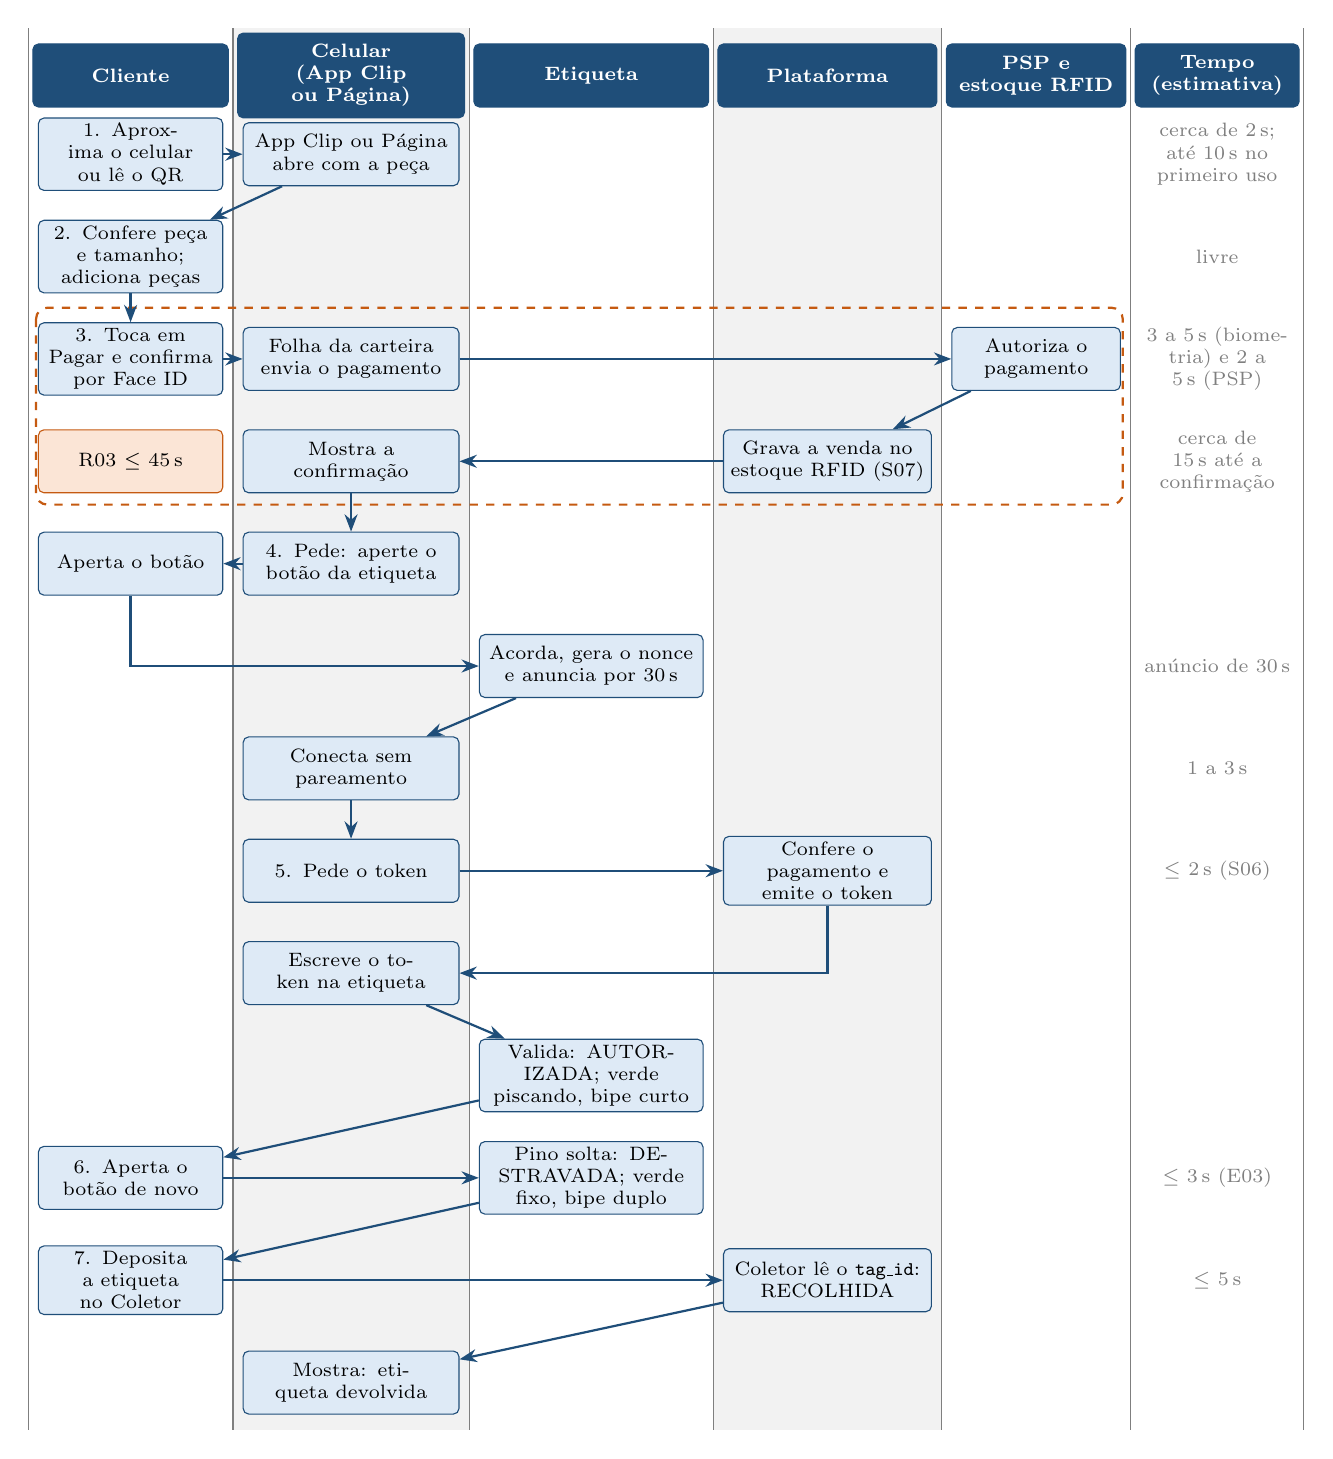
\begin{tikzpicture}[font=\scriptsize]
        % ---------------- raias ----------------
        \fill[r2cinzaclaro] (2.6,1.6) rectangle (5.6,-16.2);
        \fill[r2cinzaclaro] (8.7,1.6) rectangle (11.6,-16.2);
        \foreach \x in {0,2.6,5.6,8.7,11.6,14.0,16.2} {\draw[r2cinza] (\x,1.6) -- (\x,-16.2);}
        \node[r2blocoescuro, font=\scriptsize\bfseries, text width=2.2cm] at (1.3,1.0) {Cliente};
        \node[r2blocoescuro, font=\scriptsize\bfseries, text width=2.6cm] at (4.1,1.0) {Celular\\ (App Clip ou Página)};
        \node[r2blocoescuro, font=\scriptsize\bfseries, text width=2.7cm] at (7.15,1.0) {Etiqueta};
        \node[r2blocoescuro, font=\scriptsize\bfseries, text width=2.5cm] at (10.15,1.0) {Plataforma};
        \node[r2blocoescuro, font=\scriptsize\bfseries, text width=2.0cm] at (12.8,1.0) {PSP e estoque RFID};
        \node[r2blocoescuro, font=\scriptsize\bfseries, text width=1.8cm] at (15.1,1.0) {Tempo\\ (estimativa)};
        % ---------------- faixa de R03 ----------------
        \draw[r2laranja, dashed, thick, rounded corners] (0.1,-1.95) rectangle (13.9,-4.45);
        % ---------------- passos ----------------
        \node[r2bloco, font=\scriptsize, text width=2.2cm, inner sep=2pt] (a1) at (1.3,0) {1. Aproxima o celular ou lê o QR};
        \node[r2bloco, font=\scriptsize, text width=2.6cm, inner sep=2pt] (b1) at (4.1,0) {App Clip ou Página abre com a peça};
        \node[r2bloco, font=\scriptsize, text width=2.2cm, inner sep=2pt] (a2) at (1.3,-1.3) {2. Confere peça e tamanho; adiciona peças};
        \node[r2bloco, font=\scriptsize, text width=2.2cm, inner sep=2pt] (a3) at (1.3,-2.6) {3. Toca em Pagar e confirma por Face ID};
        \node[r2bloco, font=\scriptsize, text width=2.6cm, inner sep=2pt] (b3) at (4.1,-2.6) {Folha da carteira envia o pagamento};
        \node[r2bloco, font=\scriptsize, text width=2.0cm, inner sep=2pt] (e3) at (12.8,-2.6) {Autoriza o pagamento};
        \node[r2bloco, font=\scriptsize, text width=2.5cm, inner sep=2pt] (d4) at (10.15,-3.9) {Grava a venda no estoque RFID (S07)};
        \node[r2bloco, font=\scriptsize, text width=2.6cm, inner sep=2pt] (b4) at (4.1,-3.9) {Mostra a confirmação};
        \node[r2destaque, font=\scriptsize, text width=2.2cm, inner sep=2pt] at (1.3,-3.9) {R03 $\leq$ 45\,s};
        \node[r2bloco, font=\scriptsize, text width=2.6cm, inner sep=2pt] (b5) at (4.1,-5.2) {4. Pede: aperte o botão da etiqueta};
        \node[r2bloco, font=\scriptsize, text width=2.2cm, inner sep=2pt] (a5) at (1.3,-5.2) {Aperta o botão};
        \node[r2bloco, font=\scriptsize, text width=2.7cm, inner sep=2pt] (c6) at (7.15,-6.5) {Acorda, gera o nonce e anuncia por 30\,s};
        \node[r2bloco, font=\scriptsize, text width=2.6cm, inner sep=2pt] (b7) at (4.1,-7.8) {Conecta sem pareamento};
        \node[r2bloco, font=\scriptsize, text width=2.6cm, inner sep=2pt] (b8) at (4.1,-9.1) {5. Pede o token};
        \node[r2bloco, font=\scriptsize, text width=2.5cm, inner sep=2pt] (d8) at (10.15,-9.1) {Confere o pagamento e emite o token};
        \node[r2bloco, font=\scriptsize, text width=2.6cm, inner sep=2pt] (b9) at (4.1,-10.4) {Escreve o token na etiqueta};
        \node[r2bloco, font=\scriptsize, text width=2.7cm, inner sep=2pt] (c10) at (7.15,-11.7) {Valida: AUTORIZADA; verde piscando, bipe curto};
        \node[r2bloco, font=\scriptsize, text width=2.2cm, inner sep=2pt] (a11) at (1.3,-13.0) {6. Aperta o botão de novo};
        \node[r2bloco, font=\scriptsize, text width=2.7cm, inner sep=2pt] (c11) at (7.15,-13.0) {Pino solta: DESTRAVADA; verde fixo, bipe duplo};
        \node[r2bloco, font=\scriptsize, text width=2.2cm, inner sep=2pt] (a12) at (1.3,-14.3) {7. Deposita a etiqueta no Coletor};
        \node[r2bloco, font=\scriptsize, text width=2.5cm, inner sep=2pt] (d12) at (10.15,-14.3) {Coletor lê o \texttt{tag\_id}: RECOLHIDA};
        \node[r2bloco, font=\scriptsize, text width=2.6cm, inner sep=2pt] (b13) at (4.1,-15.6) {Mostra: etiqueta devolvida};
        % ---------------- tempos ----------------
        \node[r2rotulo, text width=1.9cm] at (15.1,0) {cerca de 2\,s; até 10\,s no primeiro uso};
        \node[r2rotulo, text width=1.9cm] at (15.1,-1.3) {livre};
        \node[r2rotulo, text width=1.9cm] at (15.1,-2.6) {3 a 5\,s (biometria) e 2 a 5\,s (PSP)};
        \node[r2rotulo, text width=1.9cm] at (15.1,-3.9) {cerca de 15\,s até a confirmação};
        \node[r2rotulo, text width=1.9cm] at (15.1,-6.5) {anúncio de 30\,s};
        \node[r2rotulo, text width=1.9cm] at (15.1,-7.8) {1 a 3\,s};
        \node[r2rotulo, text width=1.9cm] at (15.1,-9.1) {$\leq$ 2\,s (S06)};
        \node[r2rotulo, text width=1.9cm] at (15.1,-13.0) {$\leq$ 3\,s (E03)};
        \node[r2rotulo, text width=1.9cm] at (15.1,-14.3) {$\leq$ 5\,s};
        % ---------------- setas ----------------
        \draw[r2seta] (a1) -- (b1);
        \draw[r2seta] (b1) -- (a2);
        \draw[r2seta] (a2) -- (a3);
        \draw[r2seta] (a3) -- (b3);
        \draw[r2seta] (b3) -- (e3);
        \draw[r2seta] (e3) -- (d4);
        \draw[r2seta] (d4) -- (b4);
        \draw[r2seta] (b4) -- (b5);
        \draw[r2seta] (b5) -- (a5);
        \draw[r2seta] (a5.south) |- (c6.west);
        \draw[r2seta] (c6) -- (b7);
        \draw[r2seta] (b7) -- (b8);
        \draw[r2seta] (b8) -- (d8);
        \draw[r2seta] (d8.south) |- (b9.east);
        \draw[r2seta] (b9) -- (c10);
        \draw[r2seta] (c10) -- (a11);
        \draw[r2seta] (a11) -- (c11);
        \draw[r2seta] (c11) -- (a12);
        \draw[r2seta] (a12) -- (d12);
        \draw[r2seta] (d12) -- (b13);
    \end{tikzpicture}%
    }
    \source{Elaborado pelos autores (2026). Tempos estimados pela equipe, a medir no protótipo.}
\end{figure}

\subsection{Fluxo da Jornada Completa e cenários de exceção}

A parte superior da Figura~\ref{fig:r2-fluxo-completa} mostra a Jornada Completa, que roda no módulo Tag\&Go do app Riachuelo. O cliente entra no app e escolhe a loja, ou lê o QR da entrada; busca a peça e vê o setor em que ela está (nível N1) e a disponibilidade por tamanho; recebe recomendações restritas ao que existe na loja no tamanho do seu perfil; e, se o tamanho procurado faltar, faz o pedido on-line, com retirada na loja sem custo ou entrega sem frete acima de um valor mínimo a definir com a Riachuelo. O setor vem do estoque RFID e do planograma digital, sem depender da etiqueta (Subseção~\ref{sub:r2-localizar}). Em seguida, lê as etiquetas das peças para montar a sacola e paga com o cartão Riachuelo, com a carteira digital ou com Pix. A liberação repete os passos 4 a 7 da Compra Rápida, já que a etiqueta e o protocolo pertencem ao núcleo comum. Depois do registro de ``etiqueta devolvida'', o cashback do Ria Club é creditado, o que amarra o benefício ao retorno da etiqueta, e o app mostra um cartão de sustentabilidade da compra, com estimativas por categoria acompanhadas de faixa e fonte.

A parte inferior da figura trata dos oito cenários de exceção que a meta R07 obriga a cobrir com uma alternativa humana, cada um com a primeira resposta do sistema. A falta de dados móveis (X1), o celular descarregado depois do pagamento (X2) e a etiqueta sem energia ou sem resposta BLE (X3) resolvem-se no Liberador de Balcão, que energiza a etiqueta pelos contatos, entrega o token e conclui a liberação em até 60\,s depois que o funcionário localiza a compra pelo CPF, pelo e-mail da carteira ou pelo número do pedido (S09); no caso X1, o cliente pode ainda usar o Wi-Fi de convidados do Ponto de Apoio, com acesso livre aos domínios da Plataforma e do PSP (S08). O Pix pendente (X4), o token expirado (X5) e o pagamento recusado (X6) resolvem-se no próprio app, e a etiqueta segue TRAVADA até haver pagamento confirmado e token válido. A falha total da eletrônica (X7), cuja frequência deverá ficar em até 0,1\% das liberações, leva à remoção destrutiva no Ponto de Apoio, com registro, e a etiqueta sai do ciclo como REPROVADA. O alarme do pórtico com compra paga (X8) é atendido com discrição, e o app mostra o comprovante, o que responde à necessidade de concluir a compra sem constrangimento registrada no Relatório 1. Em todos os casos, o Ponto de Apoio é a última instância, o que garante os 100\% de R07.

Os cenários X1 e X2 aplicam a regra de conectividade da Subseção~\ref{sub:r2-caminhos}: a etiqueta não precisa de rede, e o celular sem dados ou sem bateria leva a compra ao Ponto de Apoio.

\begin{figure}[htbp]
    \centering
    \caption{Fluxo da Jornada Completa e cenários de exceção}
    \label{fig:r2-fluxo-completa}
    \resizebox{\textwidth}{!}{%
    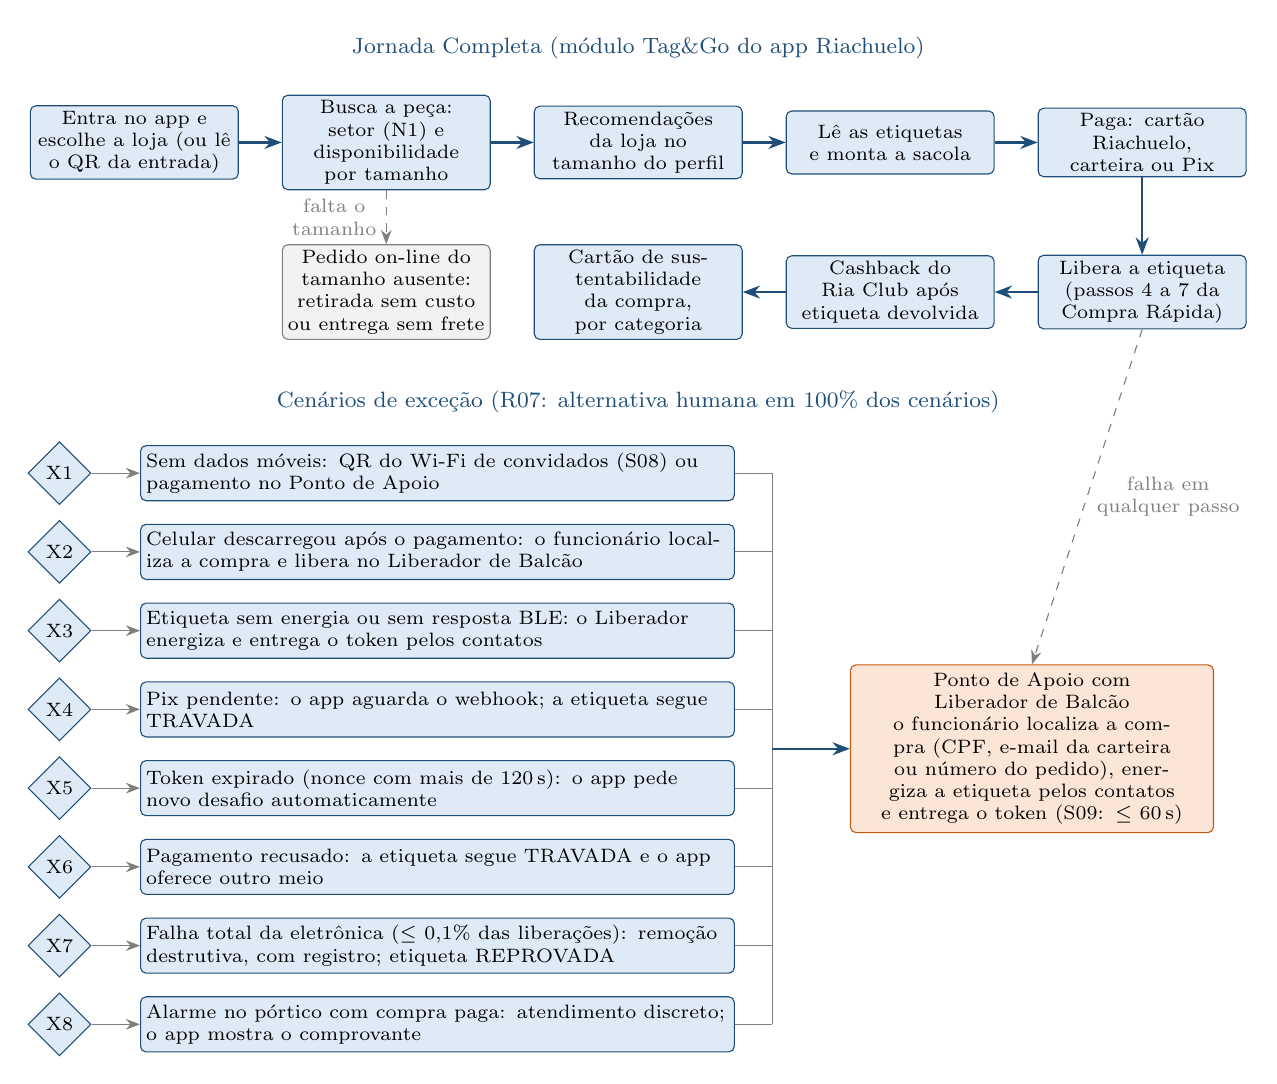
\begin{tikzpicture}[font=\scriptsize]
        % ---------------- Jornada Completa ----------------
        \node[font=\footnotesize, text=r2azul] at (7.9,1.2) {Jornada Completa (módulo Tag\&Go do app Riachuelo)};
        \node[r2bloco, font=\scriptsize, text width=2.5cm, inner sep=2pt] (j1) at (1.5,0) {Entra no app e escolhe a loja (ou lê o QR da entrada)};
        \node[r2bloco, font=\scriptsize, text width=2.5cm, inner sep=2pt] (j2) at (4.7,0) {Busca a peça: setor (N1) e disponibilidade por tamanho};
        \node[r2bloco, font=\scriptsize, text width=2.5cm, inner sep=2pt] (j3) at (7.9,0) {Recomendações da loja no tamanho do perfil};
        \node[r2bloco, font=\scriptsize, text width=2.5cm, inner sep=2pt] (j4) at (11.1,0) {Lê as etiquetas e monta a sacola};
        \node[r2bloco, font=\scriptsize, text width=2.5cm, inner sep=2pt] (j5) at (14.3,0) {Paga: cartão Riachuelo, carteira ou Pix};
        \node[r2bloco, font=\scriptsize, text width=2.5cm, inner sep=2pt] (j6) at (14.3,-1.9) {Libera a etiqueta (passos 4 a 7 da Compra Rápida)};
        \node[r2bloco, font=\scriptsize, text width=2.5cm, inner sep=2pt] (j7) at (11.1,-1.9) {Cashback do Ria Club após etiqueta devolvida};
        \node[r2bloco, font=\scriptsize, text width=2.5cm, inner sep=2pt] (j8) at (7.9,-1.9) {Cartão de sustentabilidade da compra, por categoria};
        \node[r2neutro, font=\scriptsize, text width=2.5cm, inner sep=2pt] (jo) at (4.7,-1.9) {Pedido on-line do tamanho ausente: retirada sem custo ou entrega sem frete};
        \draw[r2seta] (j1) -- (j2);
        \draw[r2seta] (j2) -- (j3);
        \draw[r2seta] (j3) -- (j4);
        \draw[r2seta] (j4) -- (j5);
        \draw[r2seta] (j5) -- (j6);
        \draw[r2seta] (j6) -- (j7);
        \draw[r2seta] (j7) -- (j8);
        \draw[r2setafina, dashed] (j2) -- node[r2rotulo, left] {falta o\\ tamanho} (jo);
        % ---------------- cenarios de excecao ----------------
        \node[font=\footnotesize, text=r2azul] at (7.9,-3.3) {Cenários de exceção (R07: alternativa humana em 100\% dos cenários)};
        \node[shape=diamond, draw=r2azul, fill=r2azulclaro, font=\scriptsize, inner sep=1pt, minimum size=8mm] (x1) at (0.55,-4.2) {X1};
        \node[shape=diamond, draw=r2azul, fill=r2azulclaro, font=\scriptsize, inner sep=1pt, minimum size=8mm] (x2) at (0.55,-5.2) {X2};
        \node[shape=diamond, draw=r2azul, fill=r2azulclaro, font=\scriptsize, inner sep=1pt, minimum size=8mm] (x3) at (0.55,-6.2) {X3};
        \node[shape=diamond, draw=r2azul, fill=r2azulclaro, font=\scriptsize, inner sep=1pt, minimum size=8mm] (x4) at (0.55,-7.2) {X4};
        \node[shape=diamond, draw=r2azul, fill=r2azulclaro, font=\scriptsize, inner sep=1pt, minimum size=8mm] (x5) at (0.55,-8.2) {X5};
        \node[shape=diamond, draw=r2azul, fill=r2azulclaro, font=\scriptsize, inner sep=1pt, minimum size=8mm] (x6) at (0.55,-9.2) {X6};
        \node[shape=diamond, draw=r2azul, fill=r2azulclaro, font=\scriptsize, inner sep=1pt, minimum size=8mm] (x7) at (0.55,-10.2) {X7};
        \node[shape=diamond, draw=r2azul, fill=r2azulclaro, font=\scriptsize, inner sep=1pt, minimum size=8mm] (x8) at (0.55,-11.2) {X8};
        \node[r2bloco, font=\scriptsize, text width=7.4cm, minimum height=7mm, inner sep=2pt, align=left] (b1) at (5.35,-4.2) {Sem dados móveis: QR do Wi-Fi de convidados (S08) ou pagamento no Ponto de Apoio};
        \node[r2bloco, font=\scriptsize, text width=7.4cm, minimum height=7mm, inner sep=2pt, align=left] (b2) at (5.35,-5.2) {Celular descarregou após o pagamento: o funcionário localiza a compra e libera no Liberador de Balcão};
        \node[r2bloco, font=\scriptsize, text width=7.4cm, minimum height=7mm, inner sep=2pt, align=left] (b3) at (5.35,-6.2) {Etiqueta sem energia ou sem resposta BLE: o Liberador energiza e entrega o token pelos contatos};
        \node[r2bloco, font=\scriptsize, text width=7.4cm, minimum height=7mm, inner sep=2pt, align=left] (b4) at (5.35,-7.2) {Pix pendente: o app aguarda o webhook; a etiqueta segue TRAVADA};
        \node[r2bloco, font=\scriptsize, text width=7.4cm, minimum height=7mm, inner sep=2pt, align=left] (b5) at (5.35,-8.2) {Token expirado (nonce com mais de 120\,s): o app pede novo desafio automaticamente};
        \node[r2bloco, font=\scriptsize, text width=7.4cm, minimum height=7mm, inner sep=2pt, align=left] (b6) at (5.35,-9.2) {Pagamento recusado: a etiqueta segue TRAVADA e o app oferece outro meio};
        \node[r2bloco, font=\scriptsize, text width=7.4cm, minimum height=7mm, inner sep=2pt, align=left] (b7) at (5.35,-10.2) {Falha total da eletrônica ($\leq$ 0,1\% das liberações): remoção destrutiva, com registro; etiqueta REPROVADA};
        \node[r2bloco, font=\scriptsize, text width=7.4cm, minimum height=7mm, inner sep=2pt, align=left] (b8) at (5.35,-11.2) {Alarme no pórtico com compra paga: atendimento discreto; o app mostra o comprovante};
        \node[r2destaque, font=\scriptsize, text width=4.4cm, inner sep=3pt] (ap) at (12.9,-7.7) {Ponto de Apoio com Liberador de Balcão\\ o funcionário localiza a compra (CPF, e-mail da carteira ou número do pedido), energiza a etiqueta pelos contatos e entrega o token (S09: $\leq$ 60\,s)};
        \foreach \i in {1,...,8} {\draw[r2setafina] (x\i.east) -- (b\i.west);}
        \foreach \i in {1,...,8} {\draw[r2cinza] (b\i.east) -- (9.6,-3.2-\i);}
        \draw[r2cinza] (9.6,-4.2) -- (9.6,-11.2);
        \draw[r2seta] (9.6,-7.7) -- (ap.west);
        \draw[r2setafina, dashed] (j6.south) -- node[r2rotulo, right] {falha em\\ qualquer passo} (ap.north);
    \end{tikzpicture}%
    }
    \source{Elaborado pelos autores (2026).}
\end{figure}

\subsection{Segurança da autorização}

A segurança do conceito parte de uma premissa conservadora: o celular do cliente é tratado como um retransmissor não confiável. Ele leva mensagens entre a etiqueta e a Plataforma, sem guardar nenhum segredo capaz de abrir a etiqueta, e a decisão de liberar é tomada pela própria etiqueta, que confere uma autorização emitida pela Plataforma para um desafio que ela mesma gerou. O protocolo tem sete passos. Na leitura, a URL traz só o \texttt{tag\_id}, e o serviço Itens e Carrinho resolve o \texttt{tag\_id} no EPC da peça e o EPC no SKU e no preço; o preço vem sempre do EPC. No pagamento, o canal paga pelo serviço Pagamento, por meio do PSP e das carteiras tokenizadas, e, confirmada a transação, a Plataforma grava a peça como vendida no estoque RFID (S07). No desafio, o cliente aperta o botão, e a etiqueta acorda, gera um nonce de 128 bits com o gerador aleatório do chip e o expõe por GATT, sem pareamento.

Na emissão, o celular envia ao serviço Autorização o \texttt{tag\_id}, o nonce e o identificador da transação. A Plataforma confere que o pagamento foi confirmado, que a associação entre o \texttt{tag\_id} e o EPC está vigente e que essa transação ainda não liberou a etiqueta; em seguida, deriva no HSM a chave da etiqueta a partir de uma chave mestra e calcula o token:
\begin{equation}
    K_{\text{tag}} = \text{HMAC}\left(K_{\text{mestra}},\ \text{tag\_id}\right)
\end{equation}
\begin{equation}
    \text{token} = \text{HMAC-SHA256}\left(K_{\text{tag}},\ \text{tag\_id} \,\|\, \text{EPC} \,\|\, \text{nonce} \,\|\, \text{transação}\right)
\end{equation}

Na validação, a etiqueta recalcula o HMAC no periférico dedicado do ESP32-C3, com a chave gravada no eFuse protegido contra leitura, que calcula o HMAC-SHA256 sem expor a chave ao software \cite{espressif2026hmac}. Ela confere também que o nonce é o atual e tem menos de 120\,s, medidos pelo relógio da própria etiqueta enquanto está acordada, o que dispensa hora absoluta, e aceita o token uma única vez. Na liberação, com o segundo aperto do botão, o pino solta, e a etiqueta descarta o nonce e registra o evento. Na devolução, no estado DESTRAVADA, a etiqueta anuncia por 10\,min para que o Coletor registre o \texttt{tag\_id} e depois entra em modo transporte, com o botão desativado; a partir daí, só acorda pelos contatos da Bandeja de Recarga ou do Liberador de Balcão.

O mesmo protocolo funciona sem o celular. No Liberador de Balcão, a etiqueta é energizada pelos contatos, e os passos de desafio, emissão, validação e liberação passam pela interface serial dos contatos. Nesse caso, quem pede o token à Plataforma é o próprio Liberador, dispositivo autenticado da loja, depois do pagamento no PDV ou de o funcionário localizar a compra feita pelo celular. A equipe manteve, assim, uma única regra de autorização para o fluxo principal e para as exceções, o que simplifica a auditoria: toda emissão de token e toda liberação ficam registradas com \texttt{tag\_id}, EPC, transação e horário (S10), à semelhança das travas eletrônicas de expositores com trilha de auditoria \cite{invue2026locks}.

A Tabela~\ref{tab:r2-ameacas} relaciona as ameaças que a equipe considerou e a resposta do projeto a cada uma. Ela servirá de roteiro para o ensaio de ataque de R06, que exige zero liberações sem pagamento confirmado em pelo menos 200 tentativas.

\begin{table}[htbp]
    \centering
    \caption{Ameaças à liberação autorizada e respostas do projeto}
    \label{tab:r2-ameacas}
    \footnotesize
    \renewcommand{\arraystretch}{1.25}
    \begin{tabularx}{\textwidth}{@{}
        >{\RaggedRight\arraybackslash}p{5.0cm}
        >{\RaggedRight\arraybackslash}X@{}}
        \toprule
        \textbf{Ameaça} & \textbf{Resposta do projeto} \\
        \midrule
        Celular modificado forja o token & o celular não tem a chave; atua só como retransmissor não confiável \\
        Repetição de um token já usado & nonce novo a cada despertar; token de uso único, válido por 120\,s \\
        Token de uma etiqueta usado em outra & chave e \texttt{tag\_id} próprios de cada etiqueta \\
        Troca de etiqueta entre peças (peça cara com a etiqueta de uma barata) & associação entre \texttt{tag\_id} e EPC no cadastro; preço sempre pelo EPC; pórtico RFID alarma se o EPC da peça que sai não estiver vendido \\
        Destacador magnético & carretel não ferromagnético (E11) \\
        Firmware trocado & Secure Boot v2 e criptografia da flash \\
        Leitura física da chave & eFuse protegido contra leitura; o periférico HMAC não expõe a chave \\
        Retransmissão do BLE a distância & sem efeito: o token só vale para o nonce daquela etiqueta, e a liberação exige o botão físico \\
        Estorno ou chargeback depois da liberação & risco financeiro residual; antifraude do PSP e carteiras tokenizadas \\
        Devolução da peça pelo cliente & a peça volta sem etiqueta; estoque de exceção de etiquetas LIVRE (até 1\% da frota), cadastradas no Liberador em modo cadastro, ou revenda só com o RFID \\
        \bottomrule
    \end{tabularx}
    \source{Elaborado pelos autores (2026) com base em \citeonline{espressif2026hmac} e \citeonline{espressif2026secureboot}.}
\end{table}

A escolha de HMAC com chave simétrica por etiqueta, em lugar de uma assinatura ECDSA, seguiu o hardware disponível. O ESP32-C3 tem periférico HMAC com chave em eFuse, Secure Boot v2 e criptografia da flash, e não lista acelerador dedicado de curvas elípticas \cite{espressif2026esp32c3, espressif2026secureboot}; como o tempo de uma verificação ECDSA nesse chip não foi medido, a equipe não o usou como critério. A derivação da chave por etiqueta limita o dano de um vazamento, já que quem extrair a chave de uma etiqueta conseguirá abrir apenas aquela etiqueta. Dois riscos ficam fora do alcance da criptografia e aparecem na tabela como residuais: o estorno depois da liberação, uma janela que o caixa com funcionário não tem, e a devolução da peça, que exige um pequeno estoque de etiquetas livres na loja.

\subsection{Ciclo da etiqueta e logística reversa}
\label{sub:r2-ciclo}

A Figura~\ref{fig:r2-ciclo} mostra o ciclo fechado da etiqueta, com os estados e as etapas logísticas. A etiqueta chega LIVRE à Estação de Cadastro, onde é fixada na peça e associada ao EPC dela, e passa a TRAVADA. Com um token válido, passa a AUTORIZADA; com o botão, a DESTRAVADA; e, se passarem 120\,s sem o botão, volta a TRAVADA. O registro no Coletor de Etiquetas ou no Liberador de Balcão a leva a RECOLHIDA, e a aprovação na Bancada de Inspeção, seguida da recarga na Bandeja de Recarga, a devolve a LIVRE. A etiqueta reprovada na Bancada sai do ciclo como REPROVADA. O estado oficial vive no serviço Ciclo da Etiqueta; a etiqueta guarda só a condição da trava, o que evita divergência entre o registro da Plataforma e o que cada unidade informa.

O cadastro foi levado para a origem, prática conhecida como \textit{source tagging}, que pode ocorrer no fabricante, no armazém, no CD ou na loja \cite{sensormatic2025sourcetagging}. A equipe definiu dois ramos. No ramo fábrica, as peças próprias, cerca de 40\% do volume vendido pela rede \cite{bloomberglinea2026riachuelo}, recebem a etiqueta e o cadastro no fim da linha da fábrica de Natal, junto ao leitor RFID de expedição que existe desde o início do projeto com a Mozaiko \cite{tiinside2022riachuelo}. No ramo CD, as peças de fornecedores nacionais e importadas, cerca de 60\%, são etiquetadas no CD de Guarulhos, de Natal ou de Manaus, na separação para a loja. A equipe preferiu a separação ao recebimento para reduzir o tempo de etiqueta parada no CD, que entra diretamente no tamanho da frota. Com os dois ramos, a loja deixa de etiquetar e de cadastrar. O ganho para a loja é tempo, não custo total zero: aplicar a etiqueta custa R\$~0,14 por peça na origem (estimativa da equipe), o mesmo que na loja.

Da origem, a etiqueta viaja presa à peça no caminhão da frota própria até a loja \cite{bloomberglinea2026riachuelo, folhape2023guararapes}, onde permanece até a venda. Depois da liberação pelo cliente, ela vai ao Coletor; quando a compra passa pelo caixa, é liberada no Liberador e guardada no caixa do PDV. As etiquetas recolhidas voltam ao CD no Malote de Retorno, no retorno do mesmo caminhão, à semelhança da recirculação de etiquetas rígidas que a Sensormatic faz com o \textit{back-haul} dos caminhões \cite{sensormatic2024recirculacao}. No CD, a Bancada de Inspeção testa botão, LED, buzzer, BLE, motor, célula e firmware, verifica a retenção por amostragem, limpa e faz a triagem; a Bandeja de Recarga recarrega 20 etiquetas por vez, em cerca de 2\,h; e a etiqueta aprovada entra na fila da Estação de Cadastro. A meta é concluir o recondicionamento em até 2 dias úteis, com pelo menos 60 etiquetas por hora por posto (S03), e reprovar no máximo 2\% das etiquetas por ciclo (E10).

Três pontos de perda foram marcados na figura. P1 é a saída do cliente com a etiqueta na sacola; P2, o extravio entre o Coletor ou o caixa e o malote; e P3, a perda no malote e no transporte. A resposta a P2 e a P3 é de controle: caixa trancado, conferência por \texttt{tag\_id} das etiquetas liberadas no Liberador, lacre numerado no malote e conferência no despacho e no recebimento. O ponto P1 depende do comportamento do cliente e é tratado pelos mecanismos M1 a M4, que sustentam a meta de retorno de 99\% (S01), contra a faixa de 80\% a 83\% observada na recirculação de etiquetas rígidas \cite{pact2026etiquetas, sensormatic2024recirculacao}. O efeito econômico de não atingir a meta está na Figura~\ref{fig:r2-custo-uso}, da Seção~\ref{sec:r2-valor}.

\begin{figure}[htbp]
    \centering
    \caption{Ciclo da etiqueta e logística reversa}
    \label{fig:r2-ciclo}
    \resizebox{\textwidth}{!}{%
    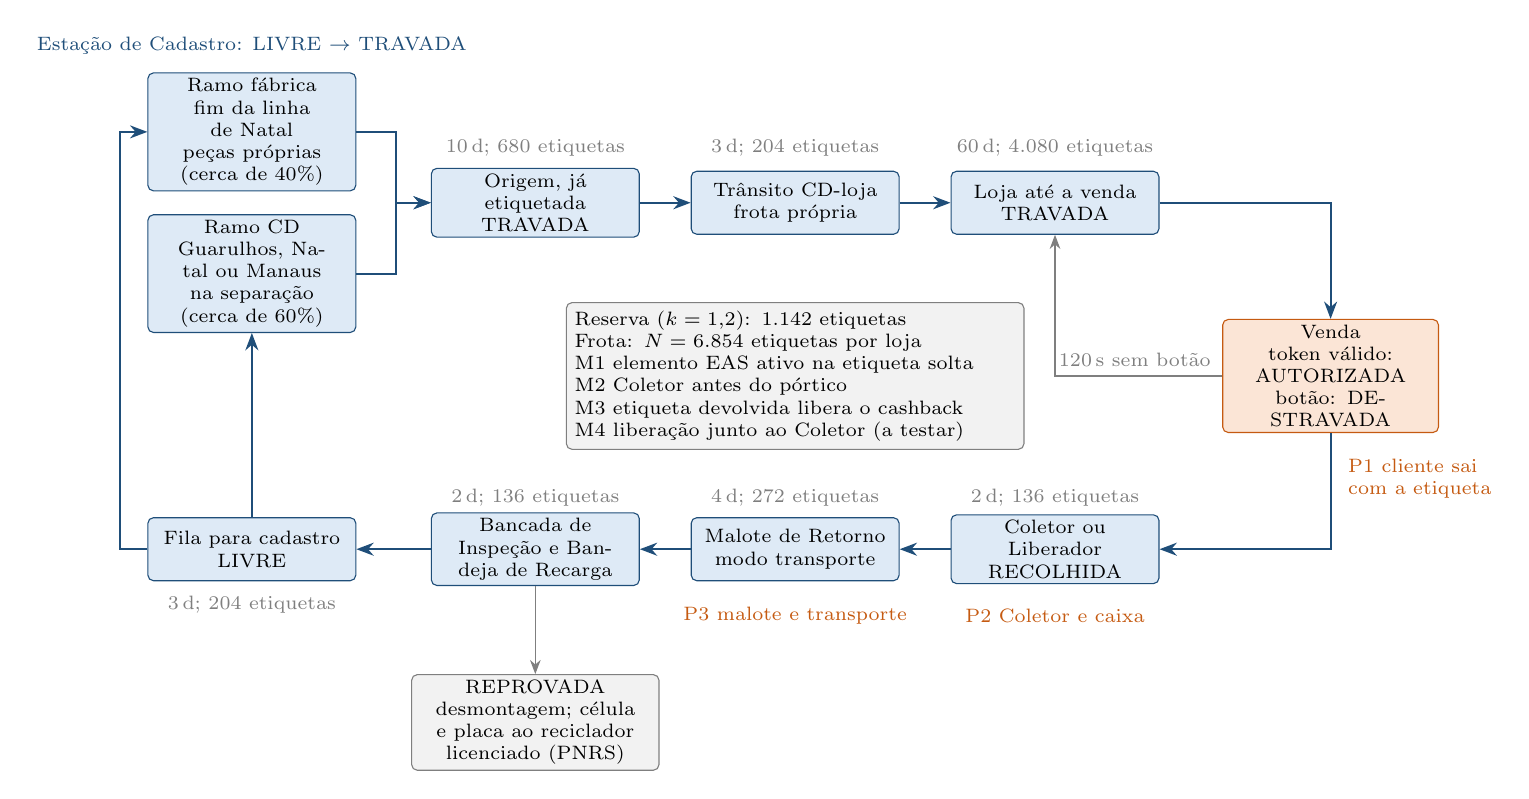
\begin{tikzpicture}[font=\scriptsize]
        % ---------------- cadastro na origem ----------------
        \node[r2rotulo, text=r2azul] at (0,6.4) {Estação de Cadastro: LIVRE $\rightarrow$ TRAVADA};
        \node[r2bloco, font=\scriptsize, text width=2.5cm, inner sep=2pt] (rf) at (0,5.3) {Ramo fábrica\\ fim da linha de Natal\\ peças próprias (cerca de 40\%)};
        \node[r2bloco, font=\scriptsize, text width=2.5cm, inner sep=2pt] (rc) at (0,3.5) {Ramo CD\\ Guarulhos, Natal ou Manaus\\ na separação (cerca de 60\%)};
        % ---------------- ida ----------------
        \node[r2bloco, font=\scriptsize, text width=2.5cm, inner sep=2pt] (or) at (3.6,4.4) {Origem, já etiquetada\\ TRAVADA};
        \node[r2bloco, font=\scriptsize, text width=2.5cm, inner sep=2pt] (tr) at (6.9,4.4) {Trânsito CD-loja\\ frota própria};
        \node[r2bloco, font=\scriptsize, text width=2.5cm, inner sep=2pt] (lj) at (10.2,4.4) {Loja até a venda\\ TRAVADA};
        \node[r2destaque, font=\scriptsize, text width=2.6cm, inner sep=2pt] (vd) at (13.7,2.2) {Venda\\ token válido: AUTORIZADA\\ botão: DESTRAVADA};
        % ---------------- volta ----------------
        \node[r2bloco, font=\scriptsize, text width=2.5cm, inner sep=2pt] (co) at (10.2,0) {Coletor ou Liberador\\ RECOLHIDA};
        \node[r2bloco, font=\scriptsize, text width=2.5cm, inner sep=2pt] (ma) at (6.9,0) {Malote de Retorno\\ modo transporte};
        \node[r2bloco, font=\scriptsize, text width=2.5cm, inner sep=2pt] (bi) at (3.6,0) {Bancada de Inspeção e Bandeja de Recarga};
        \node[r2bloco, font=\scriptsize, text width=2.5cm, inner sep=2pt] (fi) at (0,0) {Fila para cadastro\\ LIVRE};
        \node[r2neutro, font=\scriptsize, text width=3.0cm, inner sep=2pt] (rp) at (3.6,-2.2) {REPROVADA\\ desmontagem; célula e placa ao reciclador licenciado (PNRS)};
        % ---------------- tempos e etiquetas por etapa ----------------
        \node[r2rotulo] at (3.6,5.1) {10\,d; 680 etiquetas};
        \node[r2rotulo] at (6.9,5.1) {3\,d; 204 etiquetas};
        \node[r2rotulo] at (10.2,5.1) {60\,d; 4.080 etiquetas};
        \node[r2rotulo] at (10.2,0.65) {2\,d; 136 etiquetas};
        \node[r2rotulo] at (6.9,0.65) {4\,d; 272 etiquetas};
        \node[r2rotulo] at (3.6,0.65) {2\,d; 136 etiquetas};
        \node[r2rotulo] at (0,-0.7) {3\,d; 204 etiquetas};
        % ---------------- nota central ----------------
        \node[r2neutro, font=\scriptsize, text width=5.6cm, inner sep=3pt, align=left] at (6.9,2.2) {Reserva ($k = 1{,}2$): 1.142 etiquetas\\ Frota: $N = 6.854$ etiquetas por loja\\ M1 elemento EAS ativo na etiqueta solta\\ M2 Coletor antes do pórtico\\ M3 etiqueta devolvida libera o cashback\\ M4 liberação junto ao Coletor (a testar)};
        % ---------------- pontos de perda ----------------
        \node[text=r2laranja, font=\scriptsize, anchor=west, align=left] at (13.8,0.9) {P1 cliente sai\\ com a etiqueta};
        \node[text=r2laranja, font=\scriptsize] at (10.2,-0.85) {P2 Coletor e caixa};
        \node[text=r2laranja, font=\scriptsize] at (6.9,-0.85) {P3 malote e transporte};
        % ---------------- setas ----------------
        \draw[r2seta] (rf.east) -- ++(0.5,0) |- (or.west);
        \draw[r2seta] (rc.east) -- ++(0.5,0) |- (or.west);
        \draw[r2seta] (or) -- (tr);
        \draw[r2seta] (tr) -- (lj);
        \draw[r2seta] (lj.east) -| (vd.north);
        \draw[r2seta] (vd.south) |- (co.east);
        \draw[r2seta] (co) -- (ma);
        \draw[r2seta] (ma) -- (bi);
        \draw[r2seta] (bi) -- (fi);
        \draw[r2seta] (fi.north) -- (rc.south);
        \draw[r2seta] (fi.west) -- ++(-0.35,0) |- (rf.west);
        \draw[r2setafina] (bi.south) -- (rp.north);
        \draw[r2setafina] (vd.west) -| node[r2rotulo, pos=0.25, above] {120\,s sem botão} (lj.south);
    \end{tikzpicture}%
    }
    \source{Elaborado pelos autores (2026). Tempos e quantidades por loja no caso base, estimados pela equipe.}
\end{figure}

A frota por loja foi dimensionada pela lei de Little, a partir da composição do ciclo médio T por etapa. Os tempos são premissas da equipe:
\begin{equation}
    T = 10 + 3 + 60 + 2 + 4 + 2 + 3 = 84 \text{ dias}
\end{equation}
\begin{equation}
    N = S \times T \times k = 68 \times 84 \times 1{,}2 \approx 6.854 \text{ etiquetas por loja}
\end{equation}
Nessas expressões, S são as 68 liberações diárias de uma loja padrão, isto é, 10\% das 682 peças vendidas por dia, fração de peças com etiqueta rígida adotada como premissa, e o fator k de 1,2 é uma reserva para variabilidade e perdas no processo. As parcelas de T seguem a ordem das etapas da Figura~\ref{fig:r2-ciclo}, e os 10 dias na origem são a média ponderada de 20 dias no ramo fábrica e de 3 dias no ramo CD. A permanência de 60 dias em loja é a premissa mais incerta: ela equivale a cerca de dois terços do prazo médio de estoques de 95 dias da Renner no 4T25 \cite{renner2026resultados}, adotado como âncora porque o indicador da Riachuelo não foi verificado.

A Figura~\ref{fig:r2-frota} mostra onde a frota está em cada momento. A loja concentra 4.080 etiquetas (59,5\%), seguida da reserva, com 1.142 (16,7\%), e do estoque na origem, com 680 (9,9\%); as etapas de transporte, coleta, inspeção e fila somam os 13,9\% restantes. A equipe concluiu, a partir dessa composição, que, entre as etapas do ciclo, a que mais pesa no tamanho da frota é o tempo em loja, e que encurtar a logística reversa teria efeito pequeno: com permanência de 40 dias, T cai para 64 dias e a frota para 5.222 etiquetas; com 95 dias, T sobe para 119 dias e a frota para 9.710. Fora do ciclo, a fração de peças etiquetadas tem efeito ainda maior, com 3.427 etiquetas para 5\% das peças e 13.709 para 20\%. Por isso, a recomendação de usar o Tag\&Go nas peças de giro rápido que hoje já recebem etiqueta rígida, discutida na Seção~\ref{sec:r2-valor}, reduz diretamente a frota. Com o ciclo de 84 dias e a reserva, cada etiqueta faz cerca de 3,62 ciclos por ano, ou 18,1 ciclos em 5 anos de vida (E10), e é esse número, e não a resistência do mecanismo, que limita os usos de cada unidade.

\begin{figure}[htbp]
    \centering
    \caption{Composição da frota por etapa do ciclo}
    \label{fig:r2-frota}
    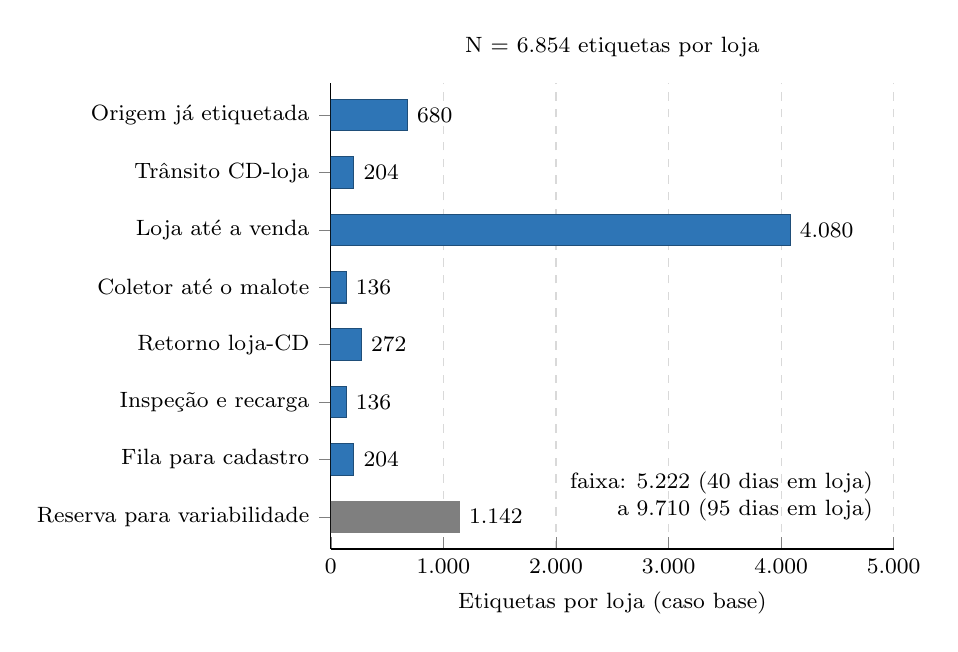
\begin{tikzpicture}
        \begin{axis}[
            r2eixo,
            xbar,
            ymajorgrids=false,
            xmajorgrids,
            width=0.72\textwidth,
            height=7.5cm,
            xmin=0, xmax=5000,
            scaled x ticks=false,
            xtick={0,1000,2000,3000,4000,5000},
            ytick={1,2,3,4,5,6,7,8},
            yticklabels={Reserva para variabilidade, Fila para cadastro, Inspeção e recarga, Retorno loja-CD, Coletor até o malote, Loja até a venda, Trânsito CD-loja, Origem já etiquetada},
            enlarge y limits=0.08,
            bar width=4mm,
            point meta=x,
            nodes near coords,
            nodes near coords align={horizontal},
            nodes near coords style={font=\footnotesize},
            xlabel={Etiquetas por loja (caso base)},
            title={N = 6.854 etiquetas por loja},
            title style={font=\footnotesize},
        ]
            \addplot[bar shift=0pt, fill=r2azulmedio, draw=r2azul] coordinates {(680,8) (204,7) (4080,6) (136,5) (272,4) (136,3) (204,2)};
            \addplot[bar shift=0pt, fill=r2cinza, draw=r2cinza] coordinates {(1142,1)};
            \node[anchor=south east, font=\footnotesize, align=right] at (rel axis cs:0.98,0.04) {faixa: 5.222 (40 dias em loja)\\ a 9.710 (95 dias em loja)};
        \end{axis}
    \end{tikzpicture}
    \source{Elaborado pelos autores (2026).}
\end{figure}

O transporte das etiquetas exige cuidado porque cada uma leva uma célula de lítio. A etiqueta viajará em modo transporte, com o botão desativado e despertar apenas pelos contatos, com a célula instalada, em caixa rígida com divisórias antiestáticas e identificação de baterias de lítio instaladas em equipamento (UN 3481). Para Manaus, a equipe recomenda o modal rodofluvial; se o transporte for aéreo, deverá seguir a instrução de embalagem para baterias instaladas em equipamento, com a carga reduzida.

No fim de vida, a etiqueta REPROVADA será desmontada na Bancada de Inspeção. A carcaça e o mecanismo serão reaproveitados quando possível, e a célula e a placa seguirão como resíduo eletroeletrônico para um reciclador licenciado, em linha com a Política Nacional de Resíduos Sólidos, que exige sistemas de logística reversa para pilhas e baterias e para produtos eletroeletrônicos \cite{brasil2010pnrs}. O Decreto 10.240/2020 trata de eletroeletrônicos de uso doméstico \cite{brasil2020decreto} e, na interpretação da equipe, que não constitui parecer jurídico, não se aplica diretamente a um ativo corporativo como a etiqueta.

\subsection{Plano macro de processo}

A fabricação da etiqueta seguirá sete etapas: injeção das duas carcaças; montagem SMT da placa única; montagem da garra, do cursor, do came e do micromotor; gravação do firmware com Secure Boot e criptografia da flash; gravação, no eFuse, da chave da etiqueta derivada no HSM; teste final de rádio, motor e retenção; e homologação na Anatel. A gravação da chave é a etapa mais sensível do processo, porque a chave mestra não pode sair do HSM, e por isso deverá ocorrer num posto controlado, com registro de cada \texttt{tag\_id} gravado. A operação, por sua vez, repete o ciclo da Figura~\ref{fig:r2-ciclo}: cadastro na origem, permanência na loja, recolhimento, malote, inspeção, recarga, fila e novo cadastro. Materiais, tolerâncias de fabricação e tempos de cada operação serão detalhados no Relatório 3, junto com as cotações de volume da célula, do micromotor e do molde.

\newpage% =============================================================================
% Relatorio 2, item F: delineamento da comercializacao e da distribuicao.
% Conteudo: cliente e unidade de decisao, canais (B2B), pontos de uso (B2C),
% distribuicao fisica da etiqueta, modalidades comerciais, cronograma (Gantt),
% riscos com LGPD e indicadores do piloto.
% Figura: fig:r2-cronograma. Tabelas: tab:r2-canais, tab:r2-riscos, tab:r2-lgpd.
% Precos e contas vem da Secao sec:r2-valor (conta_final.py); nada e recalculado.
% =============================================================================

\section{COMERCIALIZAÇÃO E DISTRIBUIÇÃO}
\label{sec:r2-comercializacao}

Com a arquitetura, os desenhos e o plano macro de processo definidos, faltava delinear como o produto chegará a quem o compra e a quem o usa, último item do projeto conceitual \cite{zancul2026conceitual}. No Tag\&Go, essas duas figuras não coincidem: quem contrata e paga pelo sistema é o varejista, e quem o usa é o consumidor da loja, que não paga nada a mais pela compra sem caixa. A equipe tratou a comercialização, por isso, como uma venda entre empresas (B2B) apoiada numa experiência de consumo (B2C), e organizou o delineamento em seis frentes: o cliente e a unidade de decisão, os canais de venda, os pontos de uso, a distribuição física da etiqueta, as modalidades comerciais com o cronograma de implantação e os riscos, entre eles o tratamento de dados pessoais. Todos os preços e resultados econômicos citados vêm da Seção~\ref{sec:r2-valor}.

\subsection{Cliente e unidade de decisão}
\label{sub:r2-cliente}

O cliente-alvo é o varejista de moda \textit{mass market} que já opera ou planeja operar o self-checkout, segmento definido no Relatório 1 e formado por Renner, Riachuelo e C\&A. A Riachuelo é o primeiro cliente pelas condições que reúne: 342 lojas da bandeira \cite{abvtex2026riachuelo}; RFID aplicado desde a expedição da fábrica de Natal, em parceria com a Mozaiko, com escopo de fábrica, CDs e lojas \cite{tiinside2022riachuelo}; lojas conceito com self-checkout, como a de Curitiba, inaugurada em abril de 2026 \cite{amanha2026riachuelo}; e o plano declarado de levar o conceito a mais de 300 unidades \cite{mercadoconsumo2026riachuelo}. Em Curitiba, a primeira loja inteiramente no novo formato registrou fluxo 15,7\% maior e faturamento 9,7\% maior, sem divulgação da base de comparação \cite{curitibainforma2026riachuelo}. O ciclo de cerca de 350 reformas e 150 lojas novas, com investimento de R\$~3 a 4~bilhões, terá avaliação financeira em abril de 2027 \cite{economicnews2026riachuelo}. A equipe concluiu, a partir dessa agenda, que a janela comercial do Tag\&Go é o próprio ciclo de reformas: o sistema precisa chegar à decisão da empresa com resultados de piloto a tempo de ser incluído nas lojas reformadas, e não depois delas.

A contratação de um sistema desse tipo envolve várias áreas da empresa. Na Riachuelo, a equipe identificou seis: Tecnologia, que recebeu a equipe em 23/09/2026 e responde pelas integrações com o estoque RFID, o PDV e o app; Operações de Loja, que responde pela rotina dos caixas e do Ponto de Apoio; Prevenção de Perdas, atenta ao efeito do autoatendimento sobre o furto; Logística e CDs, que passam a operar o ciclo da etiqueta; Marketing e CRM, responsáveis pelo app e pelo Ria Club; e o Jurídico, com o encarregado de dados, responsável pela conformidade com a LGPD. Cada área avalia o sistema por um critério próprio, e essa pluralidade levou a equipe a incluir um bloco do varejista na matriz de decisão da Seção~\ref{sec:r2-concepcao}, com peso de 25\% fixado como premissa. Como a escolha da concepção se inverte quando esse bloco pesa 36,6\% ou mais, a validação dos pesos com a empresa passa a ser o primeiro passo comercial, junto com as três premissas que dominam a conta econômica: a fração de peças com etiqueta rígida ($f$), o ciclo médio da etiqueta ($T$) e as desistências de compra evitadas por dia ($d$).

\subsection{Canais de venda}
\label{sub:r2-canais}

A equipe definiu quatro canais de venda, que entram em sequência. O primeiro é a venda direta e consultiva à Riachuelo. O caráter consultivo decorre da natureza do produto: o Tag\&Go exige integração com sistemas da empresa, muda a rotina da loja e do CD e só se justifica se o número de desistências evitadas for medido. A venda começa por um piloto numa loja conceito (Curitiba ou Oscar Freire), limitado a uma categoria de produto para conter a frota em cerca de 500 a 1.000 etiquetas (estimativa da equipe), contra as 6.854 etiquetas por loja estimadas para a operação plena na Seção~\ref{sec:r2-valor}. Confirmada a economia, o piloto dá lugar a um contrato-quadro para as 20 lojas conceito do mercado obtenível (SOM), limite superior do plano de 15 a 20 lojas no novo formato em 2026 (Subseção~\ref{sub:r2-sintese}); a Riachuelo anunciou R\$~180~milhões para 20 lojas novas em 2026 \cite{exame2026riachuelo}. Nessa escala, segundo a Seção~\ref{sec:r2-valor}, a frota soma 137.080 etiquetas e a receita do fornecedor chega a R\$~3,48~milhões por ano.

O segundo canal reúne os parceiros de integração que já atendem a Riachuelo: Mozaiko e Stefanini, no RFID e no estoque \cite{tiinside2022riachuelo}; Manhattan, no sistema de gestão de pedidos, que trata as lojas como pequenos CDs e já faz retirada e envio a partir da loja \cite{manhattan2026riachuelo}; o provedor de pagamentos (PSP) da empresa; e o fornecedor do PDV. São canais de implantação, sem papel de revenda. O Tag\&Go depende de ler o preço pelo EPC, gravar a venda no estoque RFID e emitir a NFC-e (interfaces I10 e I11 da Seção~\ref{sec:r2-arquitetura}), e as empresas que operam esses sistemas encurtam o prazo e o risco de cada integração.

O terceiro canal trata os fornecedores de etiquetas EAS como parceiros de componentes. A garra, o pino e o elemento EAS da etiqueta Tag\&Go vêm de etiquetas rígidas comerciais, e esses fornecedores já dominam a recirculação de etiquetas passivas: segundo o fornecedor, a Sensormatic recolhe as etiquetas no retorno dos caminhões, testa, limpa e reenvia às fábricas de roupa \cite{sensormatic2024recirculacao}, e a Pact opera a reutilização de etiquetas EAS \cite{pact2026etiquetas}. No futuro, parte do ciclo logístico poderá ser terceirizada a um desses parceiros.

O quarto canal é a expansão, depois da validação, para as demais redes do segmento-alvo. A Renner já tinha, no fim de 2023, autoatendimento por RFID em 213 lojas \cite{consumidormoderno2025renner} e a C\&A, self-checkout por RFID no conceito Energia \cite{brazileconomy2025cea}. A arquitetura modular permite atender essas redes mantendo a etiqueta e a Plataforma Tag\&Go e trocando só os módulos do serviço Integrações, que ligam a Plataforma ao estoque, ao PDV e ao programa de fidelidade de cada varejista.

\subsection{Pontos de venda e de uso}
\label{sub:r2-pontos}

Para o consumidor, o ponto de venda é a própria loja física, e o ponto de contato com o sistema é a etiqueta presa à peça. O Coletor de Etiquetas e o Ponto de Apoio ficam perto da saída, no caminho natural até o pórtico. Os pontos digitais variam conforme o caminho de uso. A Compra Rápida abre pelo QR ou pelo NFC da etiqueta, sem instalar app nem passar por loja de aplicativos, no App Clip Tag\&Go do iPhone ou na Página de Compra Rápida do Android (Subseção~\ref{sub:r2-caminhos}). Há, porém, uma dependência de distribuição: a Apple só publica um App Clip ligado a um app completo com pelo menos a mesma funcionalidade, no mesmo projeto \cite{apple2026appclipcriar}. A Compra Rápida no iPhone passa, portanto, pela conta de desenvolvedor da Riachuelo e pelo calendário de publicação do app da marca.

A Jornada Completa roda no módulo Tag\&Go do app Riachuelo, que já tem mais de 10~milhões de downloads e nota 4,8 no Google Play e 4,9 na App Store \cite{googleplay2026riachuelo,appstore2026riachuelo}, de modo que o módulo chega ao cliente pela base já instalada, sem canal de distribuição novo. É nesse módulo que o cliente encontra o perfil, o Ria Club, a recomendação restrita ao que existe no estoque da loja no tamanho do perfil, as métricas de sustentabilidade estimadas por categoria e a localização da peça no nível de setor (N1), função secundária que vem do estoque RFID e de um planograma digital, sem depender da etiqueta (Subseção~\ref{sub:r2-localizar}). Esse planograma é o mapa de setores que a própria loja mantém atualizado, o que acrescenta uma rotina de Operações de Loja ao contrato, e o nível de arara (N2) só entra na oferta se a Riachuelo instalar leitores RFID de teto. Para dimensionar esse caminho, a equipe adotou como referência os 4,5~milhões de clientes ativos do cartão \cite{btg2025guararapes}. Entre os dois caminhos fica o passe do Ria Club no Apple Wallet e no Google Wallet, distribuído sem app \cite{apple2026walletpass,google2026walletfidelidade}, que mantém o vínculo com o cliente da Compra Rápida. O último ponto é o e-commerce da Riachuelo, que recebe a compra on-line do tamanho ausente na loja, nas condições de retirada e de frete da Subseção~\ref{sub:r2-caminhos}, como receita incremental que não entra no equilíbrio econômico.

\subsection{Distribuição física da etiqueta}
\label{sub:r2-distribuicao}

A etiqueta Tag\&Go é um ativo retornável, e sua distribuição forma um circuito fechado entre a origem das peças e as lojas. A rota completa, com estados, tempos e pontos de perda, está na Subseção~\ref{sub:r2-ciclo} e na Figura~\ref{fig:r2-ciclo}; o delineamento comercial trata de quem transporta, onde a etiqueta é recondicionada e com que capacidade.

Na ida, a etiqueta viaja presa à peça, no caminhão da frota própria da Riachuelo, que liga a fábrica e os três CDs às lojas \cite{bloomberglinea2026riachuelo,exame2025bolsa,folhape2023guararapes}. O cadastro na origem tem dois ramos. No ramo fábrica, que cobre as peças próprias, cerca de 40\% do que a rede vende \cite{bloomberglinea2026riachuelo}, a aplicação e o cadastro acontecem no fim da linha da fábrica de Natal, junto ao leitor RFID de expedição que já existe. No ramo CD, que cobre as peças de fornecedores nacionais e importadas, a aplicação acontece no CD de Guarulhos, Natal ou Manaus, na separação para a loja. A escolha segue a prática de aplicar etiquetas na fonte, que admite quatro pontos possíveis (fabricante, armazém, CD e loja), entre os quais, segundo o fornecedor, o fabricante oferece aplicação mais consistente e menos mão de obra nas etapas seguintes \cite{sensormatic2025sourcetagging}. A aplicação continua a cargo de pessoal da Riachuelo, como hoje acontece na loja. O ganho da loja é de tempo, e o custo total da operação permanece: aplicar a etiqueta custa R\$~0,14 por peça na origem, o mesmo valor calculado para a loja na Seção~\ref{sec:r2-valor}.

Na volta, as etiquetas recolhidas seguem no Malote de Retorno, no retorno do mesmo caminhão, em modo transporte, com lacre numerado e conferência por \texttt{tag\_id} no despacho e no recebimento. No caso base, com adesão de 24\% das compras pelo celular (premissa herdada do survey do Relatório 1), cada Coletor recebe cerca de 16 etiquetas por dia e, com capacidade de cerca de 150, é esvaziado a cada 2 dias; com adesão total, recebe 68 etiquetas por dia e passa a ser esvaziado diariamente. Para Manaus, a equipe preferiu o modal rodofluvial, com as regras de transporte de baterias de lítio instaladas em equipamento descritas na Subseção~\ref{sub:r2-ciclo}.

O recondicionamento fica em dois locais: um centro no CD de Natal, junto da fábrica, onde já ocorre o cadastro do ramo fábrica, e um posto no CD de Guarulhos, perto das lojas do Sudeste, região que concentra 47\% da rede \cite{btg2025guararapes}, e das lojas do Sul. Para as 20 lojas do SOM, a equipe estimou um fluxo de 1.360 etiquetas por dia, atendido por 3 postos de inspeção (60 etiquetas por hora por posto, em 8 horas), 17 Bandejas de Recarga (20 posições e 4 ciclos por turno) e 2 Estações de Cadastro, uma na fábrica de Natal e outra no CD de Guarulhos, com cerca de 11 horas de aplicação por dia a 125 peças por hora. As etiquetas reprovadas na Bancada de Inspeção são desmontadas; carcaça e mecanismo voltam ao ciclo quando possível, e célula e placa seguem para reciclador licenciado, como exige a Política Nacional de Resíduos Sólidos para pilhas, baterias e eletroeletrônicos \cite{brasil2010pnrs}.

\subsection{Modalidades comerciais e preço}
\label{sub:r2-modalidades}

A equipe definiu duas modalidades comerciais. A principal é a locação: R\$~2,00 por etiqueta por mês, plataforma de R\$~800 por loja por mês e implantação de R\$~15.000 por loja, com franquia de perda de 1\% das liberações; acima da franquia, cada etiqueta não devolvida é cobrada a R\$~60. O preço inclui recondicionamento, recarga, reposição até a franquia, suporte, Coletores de Etiquetas, Liberadores de Balcão e os equipamentos da Estação de Cadastro. A aplicação das etiquetas na origem fica com a Riachuelo.

A locação foi escolhida como modalidade principal por três razões. A primeira é o próprio produto: a etiqueta tem custo-meta de R\$~60, contra R\$~0,87 da etiqueta rígida comum que substitui (Seção~\ref{sec:r2-valor}), e só se viabiliza como ativo reutilizável, cobrado por uso. A segunda é a divisão de riscos: na locação, o fornecedor carrega o risco de perda e de obsolescência da frota, e é ele quem pode reduzi-lo pelo projeto da etiqueta e do ciclo. A terceira é o custo para a Riachuelo. Na locação, o sistema custa R\$~7,01 por liberação, contra R\$~0,29 da etiqueta rígida atual, e a empresa empata ao evitar 3,68 desistências de compra por dia por loja, 1,6\% das 227 compras diárias estimadas. Na compra, o custo seria de R\$~6,78 por liberação sem o custo de capital da empresa e de R\$~9,28 com um custo de capital de 15\% ao ano (premissa); considerado o custo de capital, a locação é a opção mais barata para a Riachuelo e ainda a poupa de imobilizar a frota. Do lado do fornecedor, a R\$~2,00 a taxa interna de retorno em 5 anos é de 22,0\%, acima da taxa mínima de atratividade de 20\% ao ano adotada como premissa; a R\$~1,80, cairia para 16,6\% e não remuneraria o capital investido na frota.

A franquia de perda alinha os incentivos com a meta de retorno de 99\% (S01, na Tabela~\ref{tab:r2-especificacoes}). Até 1\% das liberações, a perda já está coberta pelo preço e fica com o fornecedor, que tem interesse direto em manter os mecanismos de retorno M1 a M4. Acima desse limite, a cobrança passa à Riachuelo, que tem interesse em operar o Coletor e o Ponto de Apoio com disciplina. O custo desse risco para a empresa é conhecido: com retorno de 95\%, o equilíbrio sobe para 5,05 desistências evitadas por dia por loja, e com 83\%, limite superior da faixa observada no mercado de etiquetas rígidas recirculadas, para 9,16 (Seção~\ref{sec:r2-valor}).

A compra fica como modalidade alternativa para o varejista que prefira imobilizar capital: R\$~90 por etiqueta, R\$~0,40 por ciclo de recondicionamento, mais plataforma e implantação. As duas modalidades têm precedentes no mercado. A rapitag cogitou alugar suas etiquetas aos varejistas \cite{munichstartup2017rapitag,storesshops2019rapitag}; no Brasil, o self-checkout é oferecido por compra, locação, leasing, Finame e cartão BNDES \cite{perto2021selfcheckout}; e a MishiPay, segundo o fornecedor, adota preço flexível por loja e por integração, sem valores públicos (estudos anteriores da equipe). A Tabela~\ref{tab:r2-canais} reúne cliente, canais, pontos de uso, distribuição e modalidades.

\begin{table}[htbp]
    \centering
    \caption{Canais, pontos de uso, distribuição e modalidades comerciais do Tag\&Go}
    \label{tab:r2-canais}
    \footnotesize
    \renewcommand{\arraystretch}{1.25}
    \begin{tabularx}{\textwidth}{@{}
        >{\RaggedRight\arraybackslash}p{3.2cm}
        >{\RaggedRight\arraybackslash}X@{}}
        \toprule
        \textbf{Dimensão} & \textbf{Conteúdo} \\
        \midrule
        Cliente & Varejistas de moda \textit{mass market} com self-checkout; primeiro, a Riachuelo \\
        Canal de venda & Direto e consultivo, do piloto ao contrato-quadro; parceiros de integração (Mozaiko e Stefanini, Manhattan, PSP e fornecedor do PDV); fornecedores de etiquetas EAS como parceiros de componentes \\
        Pontos de uso & Loja física (etiqueta, Coletor de Etiquetas e Ponto de Apoio); App Clip Tag\&Go e Página de Compra Rápida; módulo Tag\&Go do app Riachuelo; passe do Ria Club; e-commerce \\
        Distribuição da etiqueta & Presa à peça, da fábrica de Natal ou do CD até a loja, na frota própria; Malote de Retorno no retorno do caminhão; recondicionamento em Natal e Guarulhos \\
        Modalidade principal & Locação: R\$~2,00 por etiqueta por mês, R\$~800 por loja por mês de plataforma e R\$~15.000 de implantação por loja; franquia de perda de 1\% (acima dela, R\$~60 por etiqueta não devolvida) \\
        Modalidade alternativa & Compra: R\$~90 por etiqueta, R\$~0,40 por ciclo de recondicionamento, mais plataforma e implantação \\
        Expansão & 20 lojas conceito (SOM), a partir do 2º semestre de 2027; rede de 342 lojas Riachuelo; outras redes do segmento \\
        \bottomrule
    \end{tabularx}
    \source{Elaborado pelos autores (2026).}
\end{table}

\subsection{Implantação e cronograma}
\label{sub:r2-cronograma}

O cronograma tem dois horizontes, mostrados na Figura~\ref{fig:r2-cronograma}: o da disciplina, até dezembro de 2026, e o da implantação com a Riachuelo, a partir de 2027 \cite{zancul2026conceitual}. Em outubro de 2026, depois da aula com convidados externos de 30/09, a equipe entrega o Relatório 2 (05/10) e propõe à Riachuelo uma reunião de validação dos pesos da matriz de decisão e das premissas $f$, $T$ e $d$. Em novembro, o Relatório 3 (04/11) detalha formas, materiais e lista de materiais e acompanha o protótipo funcional. Nesse marco acontece o primeiro teste de go/no-go: verificar se o Core Bluetooth funciona num App Clip real. A documentação da Apple não inclui o Core Bluetooth entre os frameworks sem função no App Clip, mas também não afirma que ele funcione \cite{apple2026appclipfuncoes}, e o fluxo de liberação no iPhone depende dele. Seguem os ensaios de liberação condicionada ao pagamento (R06) com ataque e o Relatório 4 (23/11). Em dezembro, a equipe apresenta o relatório final com o protótipo (07 e 09/12).

A implantação começa no primeiro semestre de 2027 com o piloto numa loja conceito, limitado a uma categoria, para medir $d$, o retorno $r$, o ciclo $T$, os tempos de pagamento (R03), a conclusão sem funcionário (R04) e a adesão. O piloto coincide com a avaliação financeira do ciclo de reformas da Riachuelo, prevista para abril de 2027 \cite{economicnews2026riachuelo}, e pode alimentá-la. No segundo semestre de 2027, o sistema chega às 20 lojas do SOM, com os centros de recondicionamento de Natal e Guarulhos em operação. De 2028 em diante, a conversão acompanha o ciclo de reformas. Se o piloto medir um número de desistências evitadas abaixo do equilíbrio, uma loja poderá começar pela alternativa A2 Estação Inteligente, cujo custo de implantação é de R\$~28.877 por loja (Seção~\ref{sec:r2-concepcao}), e migrar para a etiqueta ativa quando a economia se confirmar.

\begin{figure}[htbp]
    \centering
    \caption{Cronograma de implantação}
    \label{fig:r2-cronograma}
    \resizebox{\textwidth}{!}{%
    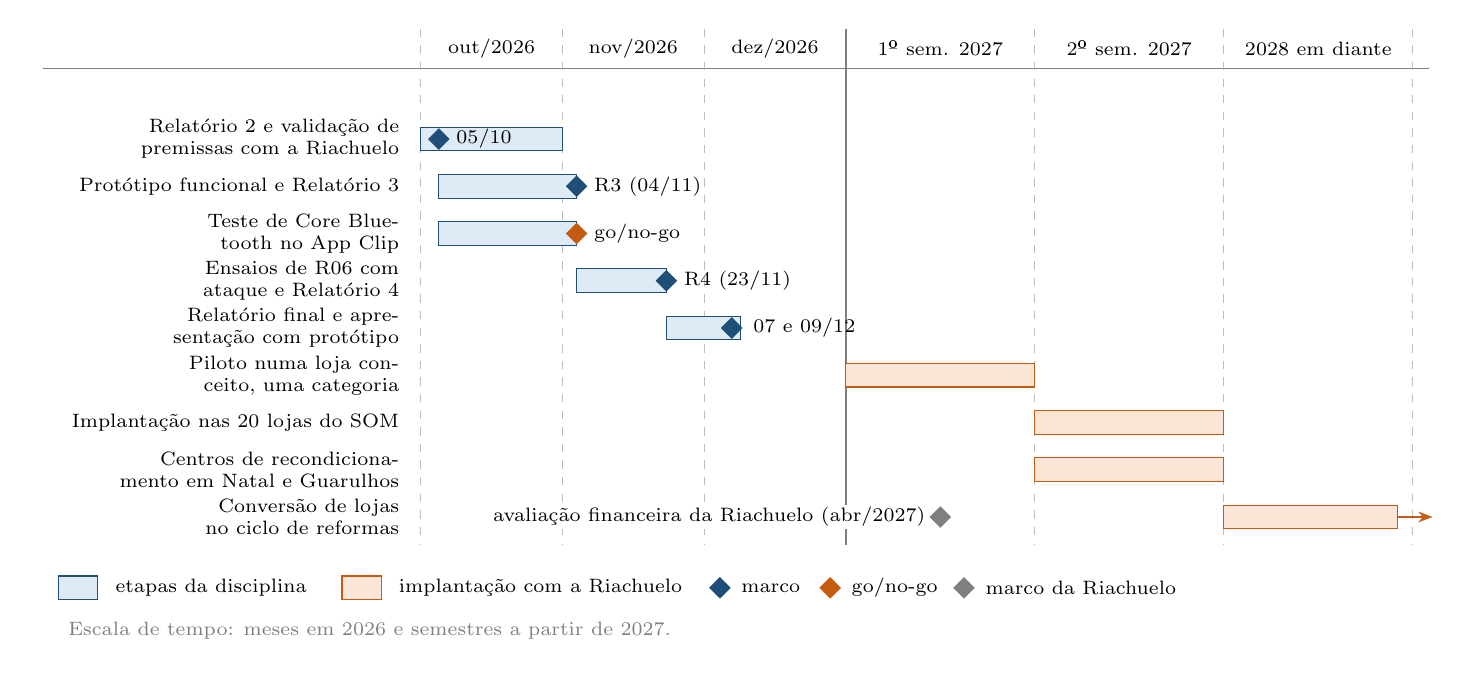
\begin{tikzpicture}[x=1cm, y=1cm, font=\scriptsize]
        % cabecalho da escala de tempo (meses em 2026; semestres a partir de 2027)
        \node at (0.9,0.55) {out/2026};
        \node at (2.7,0.55) {nov/2026};
        \node at (4.5,0.55) {dez/2026};
        \node at (6.6,0.55) {1º sem. 2027};
        \node at (9.0,0.55) {2º sem. 2027};
        \node at (11.4,0.55) {2028 em diante};
        \draw[r2cinza] (-4.8,0.3) -- (12.8,0.3);
        % divisas das colunas
        \foreach \xc in {0,1.8,3.6,7.8,10.2,12.6} {
            \draw[dashed, r2cinza!50] (\xc,0.8) -- (\xc,-5.75);
        }
        \draw[r2cinza, thick] (5.4,0.8) -- (5.4,-5.75);
        % rotulos das linhas
        \node[anchor=east, text width=4.6cm, align=right] at (-0.15,-0.6) {Relatório 2 e validação de premissas com a Riachuelo};
        \node[anchor=east, text width=4.6cm, align=right] at (-0.15,-1.2) {Protótipo funcional e Relatório 3};
        \node[anchor=east, text width=4.6cm, align=right] at (-0.15,-1.8) {Teste de Core Bluetooth no App Clip};
        \node[anchor=east, text width=4.6cm, align=right] at (-0.15,-2.4) {Ensaios de R06 com ataque e Relatório 4};
        \node[anchor=east, text width=4.6cm, align=right] at (-0.15,-3.0) {Relatório final e apresentação com protótipo};
        \node[anchor=east, text width=4.6cm, align=right] at (-0.15,-3.6) {Piloto numa loja conceito, uma categoria};
        \node[anchor=east, text width=4.6cm, align=right] at (-0.15,-4.2) {Implantação nas 20 lojas do SOM};
        \node[anchor=east, text width=4.6cm, align=right] at (-0.15,-4.8) {Centros de recondicionamento em Natal e Guarulhos};
        \node[anchor=east, text width=4.6cm, align=right] at (-0.15,-5.4) {Conversão de lojas no ciclo de reformas};
        % barras da disciplina (2026)
        \draw[draw=r2azul, fill=r2azulclaro] (0.00,-0.75) rectangle (1.80,-0.45);
        \draw[draw=r2azul, fill=r2azulclaro] (0.23,-1.35) rectangle (1.98,-1.05);
        \draw[draw=r2azul, fill=r2azulclaro] (0.23,-1.95) rectangle (1.98,-1.65);
        \draw[draw=r2azul, fill=r2azulclaro] (1.98,-2.55) rectangle (3.12,-2.25);
        \draw[draw=r2azul, fill=r2azulclaro] (3.12,-3.15) rectangle (4.06,-2.85);
        % barras da implantacao com a Riachuelo
        \draw[draw=r2laranja, fill=r2laranjaclaro] (5.40,-3.75) rectangle (7.80,-3.45);
        \draw[draw=r2laranja, fill=r2laranjaclaro] (7.80,-4.35) rectangle (10.20,-4.05);
        \draw[draw=r2laranja, fill=r2laranjaclaro] (7.80,-4.95) rectangle (10.20,-4.65);
        \draw[draw=r2laranja, fill=r2laranjaclaro] (10.20,-5.55) rectangle (12.40,-5.25);
        \draw[-{Stealth[length=1.8mm]}, thick, draw=r2laranja] (12.40,-5.40) -- (12.85,-5.40);
        % marcos
        \node[diamond, draw=r2azul, fill=r2azul, inner sep=0pt, minimum size=2.6mm] at (0.23,-0.6) {};
        \node[anchor=west] at (0.33,-0.6) {05/10};
        \node[diamond, draw=r2azul, fill=r2azul, inner sep=0pt, minimum size=2.6mm] at (1.98,-1.2) {};
        \node[anchor=west] at (2.08,-1.2) {R3 (04/11)};
        \node[diamond, draw=r2laranja, fill=r2laranja, inner sep=0pt, minimum size=2.6mm] at (1.98,-1.8) {};
        \node[anchor=west] at (2.08,-1.8) {go/no-go};
        \node[diamond, draw=r2azul, fill=r2azul, inner sep=0pt, minimum size=2.6mm] at (3.12,-2.4) {};
        \node[anchor=west] at (3.22,-2.4) {R4 (23/11)};
        \node[diamond, draw=r2azul, fill=r2azul, inner sep=0pt, minimum size=2.6mm] at (3.95,-3.0) {};
        \node[anchor=west] at (4.10,-3.0) {07 e 09/12};
        \node[diamond, draw=r2cinza, fill=r2cinza, inner sep=0pt, minimum size=2.6mm] at (6.60,-5.4) {};
        \node[anchor=east, fill=white, inner sep=1pt] at (6.45,-5.4) {avaliação financeira da Riachuelo (abr/2027)};
        % legenda
        \draw[draw=r2azul, fill=r2azulclaro] (-4.60,-6.45) rectangle (-4.10,-6.15);
        \node[anchor=west] at (-4.00,-6.3) {etapas da disciplina};
        \draw[draw=r2laranja, fill=r2laranjaclaro] (-1.00,-6.45) rectangle (-0.50,-6.15);
        \node[anchor=west] at (-0.40,-6.3) {implantação com a Riachuelo};
        \node[diamond, draw=r2azul, fill=r2azul, inner sep=0pt, minimum size=2.6mm] at (3.80,-6.3) {};
        \node[anchor=west] at (3.95,-6.3) {marco};
        \node[diamond, draw=r2laranja, fill=r2laranja, inner sep=0pt, minimum size=2.6mm] at (5.20,-6.3) {};
        \node[anchor=west] at (5.35,-6.3) {go/no-go};
        \node[diamond, draw=r2cinza, fill=r2cinza, inner sep=0pt, minimum size=2.6mm] at (6.90,-6.3) {};
        \node[anchor=west] at (7.05,-6.3) {marco da Riachuelo};
        \node[r2rotulo, anchor=west] at (-4.60,-6.85) {Escala de tempo: meses em 2026 e semestres a partir de 2027.};
    \end{tikzpicture}%
    }
    \source{Elaborado pelos autores (2026) com base em \citeonline{zancul2026conceitual} e \citeonline{economicnews2026riachuelo}.}
\end{figure}

\subsection{Riscos e mitigação}
\label{sub:r2-riscos}

A equipe reuniu os riscos da comercialização em três grupos, na Tabela~\ref{tab:r2-riscos}: econômicos, tecnológicos e de plataforma, e regulatórios. O grupo econômico é o mais sensível, porque, na análise de sensibilidade da Seção~\ref{sec:r2-valor}, a equipe concluiu que o equilíbrio da Riachuelo depende sobretudo de três variáveis: a fração de peças com etiqueta, a taxa de retorno e as perdas. As mitigações desse grupo têm, por isso, dois alvos. O primeiro é medir cedo, no piloto, o número de desistências evitadas, que hoje é a maior incerteza do modelo. O segundo é reduzir a exposição: usar o Tag\&Go só nas peças que hoje já recebem etiqueta rígida, de preferência as de maior valor e giro rápido, o que reduz $f$ e $T$ e, com eles, a frota. O mesmo grupo inclui o risco de perdas maiores com o autoatendimento: o relatório do ECR de 2026 registrou perdas 33\% maiores nas lojas com self-checkout \cite{ecr2026selfcheckout}, e por isso o caso base não conta redução de perdas; no cenário pessimista, o equilíbrio sobe para 6,6 a 8,3 desistências evitadas por dia por loja. A barreira física autenticada na peça e o pórtico RFID, que alarma quando o EPC da peça que sai não está marcado como vendido, são a resposta de projeto a esse risco.

Os riscos tecnológicos concentram-se nas plataformas móveis, fora do controle da equipe. O mais grave é a indisponibilidade do Core Bluetooth no App Clip, que deixaria a Compra Rápida no iPhone sem liberação na própria peça; a alternativa já prevista é pagar no App Clip e liberar no Liberador de Balcão. No Android, o Web Bluetooth só existe no Chrome e no Samsung Internet \cite{chrome2026webbluetooth}, e as permissões do primeiro uso podem piorar o tempo e a clareza do fluxo. Os riscos regulatórios são mais previsíveis, porque têm norma e procedimento conhecidos: a homologação na Anatel, facilitada pelo módulo com certificado \cite{espressif2026certificados} e que ainda exige avaliação do produto final por organismo certificador designado \cite{anatel2019res715}; o transporte de baterias de lítio; e a propriedade intelectual. Nesse último ponto, a família da patente US~10.121.339~B2 não tem publicação brasileira no Google Patents \cite{googlepatents2018us10121339}; a ausência ainda precisa ser confirmada no INPI, tarefa prevista para o Relatório 3 (Seção~\ref{sec:r2-aproveitamento}).

\begingroup
\footnotesize
\setlength{\tabcolsep}{4pt}
\renewcommand{\arraystretch}{1.25}
\begin{longtable}{@{}
    >{\RaggedRight\arraybackslash}p{3.6cm}
    >{\RaggedRight\arraybackslash}p{4.8cm}
    >{\RaggedRight\arraybackslash}p{6.9cm}@{}}
\caption{Riscos da comercialização e mitigação} \label{tab:r2-riscos} \\
\toprule
\textbf{Risco} & \textbf{Efeito} & \textbf{Mitigação} \\
\midrule
\endfirsthead
\multicolumn{3}{c}{Tabela~\ref{tab:r2-riscos} (continuação)} \\
\toprule
\textbf{Risco} & \textbf{Efeito} & \textbf{Mitigação} \\
\midrule
\endhead
\midrule
\multicolumn{3}{r}{\textit{continua na próxima página}} \\
\endfoot
\bottomrule
\multicolumn{3}{c}{Fonte: Elaborado pelos autores (2026).} \\
\endlastfoot
\multicolumn{3}{@{}l}{\cellcolor{r2cinzaclaro}Econômicos} \\
Retorno abaixo da meta de 99\% & Equilíbrio sobe para 5,05 (retorno de 95\%) ou 9,16 (83\%) desistências evitadas por dia por loja & Mecanismos M1 a M4; franquia de perda e cobrança por etiqueta não devolvida; painel de frota no Ponto de Apoio \\
Desistências evitadas abaixo do equilíbrio (3,7 por dia por loja) & A Riachuelo não recupera o custo da locação & Piloto com medição; uso seletivo por categoria ($f$ e $T$ menores); A2 Estação Inteligente como etapa intermediária \\
Perdas maiores com autoatendimento (ECR 2026) & Equilíbrio de 6,6 a 8,3 no cenário pessimista & Barreira física autenticada; pórtico RFID com EPC vendido; monitoramento das perdas por loja \\
Custo-meta não atingido & Taxa interna de retorno do fornecedor cai para 17,3\% com custo de R\$~66 por etiqueta & \textit{Design to cost}; cotações de volume da célula, do micromotor e do molde no Relatório 3 \\
Adesão abaixo de 24\% & Benefícios menores de tempo de caixa e de retirada da etiqueta & Jornada Completa com Ria Club; Compra Rápida como via rápida opcional \\
\multicolumn{3}{@{}l}{\cellcolor{r2cinzaclaro}Tecnológicos e de plataforma} \\
Core Bluetooth indisponível no App Clip & Compra Rápida no iPhone sem liberação na peça & Marco de go/no-go no Relatório 3; alternativa: pagar no App Clip e liberar no Liberador de Balcão \\
Atrito do Web Bluetooth e das permissões no Android & Tempo (R03) e clareza (R05) piores & Seletor filtrado pelo \texttt{tag\_id}; medição do tempo por etapa; opção de abrir no Chrome \\
Pix assíncrono & Espera pela luz verde até a confirmação do banco & Tempo de liquidação fora de R03; aviso claro na tela \\
Dependência do app Riachuelo & O App Clip exige o app publicado com a mesma função & Cronograma conjunto com o time de iOS da marca \\
\multicolumn{3}{@{}l}{\cellcolor{r2cinzaclaro}Regulatórios e jurídicos} \\
Propriedade intelectual (US~10.121.339~B2 e outras) & Restrição à exportação para os países da família de patentes & Busca no INPI no Relatório 3; diferenciação técnica (Seção~\ref{sec:r2-aproveitamento}) \\
Homologação na Anatel & Atraso do lançamento & Módulo com certificado; avaliação do produto final por organismo certificador designado \\
LGPD & Multa de até 2\% do faturamento, limitada a R\$~50~milhões por infração; perda de confiança do cliente & Base legal por finalidade (Tabela~\ref{tab:r2-lgpd}); opt-in separado; relatório de impacto à proteção de dados \\
Baterias de lítio no transporte & Risco de segurança e de conformidade & Modo transporte; embalagem rígida com divisórias; identificação UN~3481; modal rodofluvial para Manaus \\
\end{longtable}
\endgroup

\subsubsection{Dados pessoais e LGPD}
\label{sub:r2-lgpd}

O tratamento de dados pessoais é o risco regulatório que mais depende do desenho do produto, e a equipe o tratou por finalidade, como pede a LGPD. Para cada finalidade, a Tabela~\ref{tab:r2-lgpd} indica os dados necessários, a base legal e o caminho de uso em que o tratamento ocorre. O princípio que orientou a tabela é o da necessidade (art.~6º, III): cada caminho coleta só o que precisa \cite{brasil2018lgpd}. A Compra Rápida trata o mínimo para processar a compra, liberar a peça e emitir a NFC-e, com CPF opcional e e-mail apenas quando o cliente pede o recibo. A biometria usada na confirmação da carteira digital fica no aparelho e não chega à Riachuelo. A Jornada Completa, que trata perfil, histórico e dependentes, pede consentimento separado para cada finalidade, porque autorizações genéricas são nulas (art.~8º, §4º), e oferece a revogação em um toque, gratuita e facilitada (art.~8º, §5º).

\begin{table}[htbp]
    \centering
    \caption{Tratamento de dados pessoais por finalidade e base legal}
    \label{tab:r2-lgpd}
    \scriptsize
    \setlength{\tabcolsep}{4pt}
    \renewcommand{\arraystretch}{1.25}
    \begin{tabularx}{\textwidth}{@{}
        >{\RaggedRight\arraybackslash}p{2.3cm}
        >{\RaggedRight\arraybackslash}X
        >{\RaggedRight\arraybackslash}X
        >{\RaggedRight\arraybackslash}p{1.8cm}
        >{\RaggedRight\arraybackslash}X@{}}
        \toprule
        \textbf{Finalidade} & \textbf{Dados} & \textbf{Base legal (LGPD)} & \textbf{Caminho} & \textbf{Observação} \\
        \midrule
        Processar a compra e liberar a peça & Itens (EPC), \texttt{tag\_id}, identificador tokenizado do pagamento, transação & Execução de contrato (art.~7º, V) & Ambos & Dado mínimo (art.~6º, III); a biometria da carteira fica no aparelho e não chega à Riachuelo \\
        Emitir a NFC-e & Itens, valor e CPF, se o cliente pedir & Obrigação legal (art.~7º, II) & Ambos & CPF opcional \\
        Recibo por e-mail & E-mail informado na carteira (\texttt{emailRequired}) ou digitado & Execução de contrato (art.~7º, V) & Compra Rápida & Só se o cliente pedir \\
        Prevenção a fraude e auditoria & Registros de token e de liberação, horário e loja & Legítimo interesse (art.~7º, IX), com teste de balanceamento & Ambos & Retenção limitada; guia da ANPD na versão consultada em 25/09/2026 \\
        Perfil, recomendação e métricas & Tamanhos, preferências, histórico e dependentes & Consentimento (art.~7º, I) com opt-in separado por finalidade (art.~8º, §4º) e revogação em um toque (art.~8º, §5º); ou legítimo interesse com teste de balanceamento e direito de oposição & Jornada Completa & Revisão de decisões automatizadas (art.~20) se afetarem o cliente; sem preço diferenciado por perfil \\
        Fidelidade (Ria Club) & CPF, compras e cashback & Execução do contrato do programa (art.~7º, V) & Jornada Completa e passe & Regras do regulamento do programa \\
        Marketing & Contato e preferências & Consentimento (art.~7º, I) & Jornada Completa & Opt-in próprio \\
        \bottomrule
    \end{tabularx}
    \source{Elaborado pelos autores (2026) com base em \citeonline{brasil2018lgpd}, \citeonline{anpd2024legitimo} e \citeonline{midway2026riaclub}.}
\end{table}

Duas finalidades pedem cuidado adicional. A prevenção a fraude e a auditoria das liberações usam o legítimo interesse como base, o que exige finalidade legítima e específica, teste de balanceamento documentado e respeito ao direito de oposição, conforme o guia orientativo da ANPD \cite{anpd2024legitimo}; a retenção desses registros será limitada ao necessário para a auditoria. A recomendação de peças, por sua vez, é uma decisão automatizada baseada em perfil de consumo, e o titular pode pedir sua revisão (art.~20); a equipe definiu que o perfil não será usado para diferenciar preços.

Na divisão de papéis, a Riachuelo é a controladora dos dados, e o fornecedor do Tag\&Go atua como operador (art.~39), sob as instruções dela; a empresa mantém o encarregado (art.~41) e o dever de comunicar incidentes de segurança (art.~48). Se a Plataforma for hospedada em nuvem fora do país, a transferência internacional deverá seguir os arts.~33 a 36. Os direitos do titular, como acesso, correção, portabilidade e exclusão (art.~18), ficarão reunidos numa área de privacidade do app. A equipe descartou o pagamento facial próprio, adotado pela C\&A no C\&A Pay \cite{mobiletime2023cea}, porque a biometria é dado sensível (art.~11) e aumentaria o risco sem ganho para o fluxo, já que as carteiras digitais resolvem a confirmação no próprio aparelho. A preocupação com a privacidade apareceu nas entrevistas do Relatório 1, no desejo de privacidade quanto a dados de comportamento em produtos conectados (D07). Como a multa pode chegar a 2\% do faturamento, limitada a R\$~50~milhões por infração (art.~52, II), o próximo passo é elaborar, com o Jurídico da Riachuelo, o relatório de impacto à proteção de dados (RIPD) antes do piloto.

\subsection{Indicadores do piloto}
\label{sub:r2-indicadores}

O piloto só cumpre sua função comercial se medir as variáveis que decidem a economia e as especificações-meta que decidem a experiência. A equipe definiu nove indicadores. Os três primeiros são econômicos: a taxa de retorno por loja, comparada à meta S01 de 99\%; o ciclo médio da etiqueta, comparado à meta S02 de até 84 dias; e as desistências de compra evitadas, estimadas por um protocolo a combinar com a Riachuelo e comparadas ao equilíbrio de 3,7 por dia por loja. Os quatro seguintes medem a experiência: o tempo por etapa do pagamento (R03), a conclusão sem funcionário (R04), a conclusão na primeira tentativa (R05) e a adesão à compra pelo celular, comparada aos 24\% adotados como premissa. Os dois últimos são operacionais: as falhas registradas em cada cenário de exceção, de X1 a X8, e a satisfação do cliente. Com esses indicadores, a Riachuelo poderá decidir a expansão para as 20 lojas do SOM com base em resultados medidos na própria operação, e a equipe poderá substituir por medições as premissas que hoje sustentam a Seção~\ref{sec:r2-valor}.

\newpage% =============================================================================
% Consideracoes finais do Relatorio 2 (projeto conceitual do sistema Tag&Go).
% Sintese dos itens A a F com os numeros-chave, limitacoes e proximos passos.
% Sem figuras nem tabelas; os numeros sao os das Secoes 1 a 8 (biblia, 2.11).
% =============================================================================

\section{CONSIDERAÇÕES FINAIS}
\label{sec:r2-consideracoes}

No Relatório 2, a equipe percorreu os seis itens do projeto conceitual previstos no roteiro da disciplina \cite{zancul2026conceitual} e transformou a proposta do Relatório 1, uma etiqueta antifurto que o próprio cliente libera depois de pagar pelo celular, no conceito de um sistema completo, o Tag\&Go. O sistema reúne uma etiqueta ativa e reutilizável, a Plataforma Tag\&Go e seus serviços, dois caminhos de uso sobre um núcleo comum, uma infraestrutura de loja que atende às exceções e um ciclo logístico que devolve as etiquetas à fábrica ou ao centro de distribuição, onde elas são inspecionadas, recarregadas e cadastradas em novas peças. A Compra Rápida dispensa a instalação de aplicativo: o cliente abre o App Clip Tag\&Go no iPhone ou a Página de Compra Rápida no navegador do Android e paga com Apple Pay, Google Pay, cartão ou Pix copia e cola. A Jornada Completa roda no módulo Tag\&Go do app Riachuelo e acrescenta perfil, Ria Club, recomendação restrita ao estoque da loja no tamanho do perfil, compra on-line do tamanho ausente, com retirada na loja ou entrega sem frete acima de um valor mínimo, e métricas de sustentabilidade estimadas por categoria. Antes dos seis itens, a equipe corrigiu o único ponto em que o Relatório 1 perdeu nota e reescreveu as especificações-meta em três famílias, com sete requisitos do cliente (R01 a R07), doze especificações da etiqueta (E01 a E12) e dez especificações do sistema e do serviço (S01 a S10), cada uma com grandeza, unidade, valor-meta com tolerância e método de verificação (Tabela~\ref{tab:r2-especificacoes}).

\subsection{Síntese dos resultados}

Na análise funcional (Seção~\ref{sec:r2-funcional}), a equipe definiu a função global como liberar peça mediante pagamento (F0) e a representou numa caixa-preta com os fluxos de energia, material e sinal que atravessam a fronteira do sistema. Das duas estruturas funcionais comparadas, a liberação na própria peça (EF-1) foi reprovada em R07, por não oferecer caminho quando a etiqueta ou o celular falham, e a liberação em ponto fixo (EF-2) ficou fraca nos requisitos que motivaram o projeto, o tempo de pagamento (R03) e a compra sem funcionário (R04). A equipe escolheu, por isso, a estrutura mista EF-M, com liberação na peça no fluxo principal e liberação assistida no Ponto de Apoio para todas as falhas, e a desdobrou em 31 funções além da global: seis básicas (F1 a F6), 19 secundárias necessárias, três acessórias e três de estima. As seis básicas pertencem ao núcleo comum, o que confirma que os dois caminhos diferem apenas em funções secundárias. A localização do produto na loja (F25) foi mantida como secundária acessória, removível sem afetar F0. Entre os quatro níveis de granularidade avaliados, da unidade (N0) à peça (N3), a equipe adotou o N1, o setor e o piso, obtido do estoque RFID e de um planograma digital, sem depender da etiqueta; quando a leitura RFID tem mais de 24 horas ou apresenta divergência, o app indica a disponibilidade como ``provável'' e oferece a compra on-line. O N2 ficou como evolução, caso a Riachuelo instale leitores de teto, e a etiqueta como farol de rádio foi rejeitada porque, pela estimativa da equipe, esgotaria a célula em cerca de 16 dias, menos que um ciclo. As funções do ciclo da etiqueta (F17 a F24) registram a mudança mais profunda em relação ao Relatório 1: a etiqueta deixou de ser consumível e passou a ser um ativo retornável.

No estudo de diferenciação (Seção~\ref{sec:r2-diferenciacao}), a equipe comparou o Tag\&Go com dez referências em sete atributos, da rede tradicional e das lojas conceito da Riachuelo a soluções de outros mercados, como MishiPay, Paytag, rapitag e Sensormatic SuperTag 4. No mapa de posicionamento, construído com posições estimadas pela equipe, o quadrante que combina liberação sem ponto fixo e barreira autenticada na peça ficou com apenas duas soluções: a rapitag, que exige o app do varejista, e o Tag\&Go. A equipe formulou cinco diferenciais (DF1 a DF5), cada um pelo contraste com uma referência concreta: pagamento em qualquer ponto da loja com liberação na própria peça; autorização verificada na etiqueta, com imunidade ao destacador magnético; Compra Rápida sem instalar aplicativo nas duas plataformas; ciclo fechado de uma etiqueta ativa com cadastro na origem; e Jornada Completa ligada ao Ria Club. Registrou também o que não diferencia o produto, como o self-checkout em si, o RFID, a carteira digital e o cashback, que o mercado já oferece. Os riscos de diferenciação são a entrada da Paytag ou da rapitag no Brasil e a tecnologia não divulgada das lojas conceito da Riachuelo, que pode já cobrir parte do DF1.

Na escala vertical e no valor mercadológico (Seção~\ref{sec:r2-valor}), a equipe tratou o valor como uma questão de viabilidade para dois agentes, a Riachuelo e o fornecedor, porque o Tag\&Go é vendido a um varejista e não tem concorrente direto à venda no Brasil. A escala de 25 itens, com 23 produtos de referência em cinco categorias, posicionou o custo-meta de R\$~60 entre as etiquetas eletrônicas de prateleira (R\$~26,00 a R\$~51,99) e os rastreadores BLE de consumo (R\$~129,93 a R\$~369,00), posição coerente com um dispositivo que tem rádio, bateria e atuador. Como a etiqueta custa cerca de 70 vezes a mini tag que substitui, a equipe concluiu que ela só se viabiliza como ativo reutilizável, cobrado por uso. O custo-meta foi fixado em R\$~60 $\pm$ 10\%, com composição de R\$~63,25, contra R\$~122,00 na escala sem redesenho e R\$~136,21 no protótipo; a redução de 48,2\% veio de três decisões de projeto, a célula menor, o micromotor com came e a placa única. A frota foi dimensionada, como premissa, em 6.854 etiquetas por loja ($68 \times 84 \times 1{,}2$). Na locação, modalidade principal, a Riachuelo paga R\$~2,00 por etiqueta por mês, R\$~800 por mês pela plataforma e R\$~15.000 de implantação por loja, o que equivale a R\$~7,01 por liberação, contra R\$~0,29 com a etiqueta rígida atual, e empata ao evitar 3,68 desistências de compra por dia por loja, 1,6\% das 227 compras diárias estimadas. Para o fornecedor, esse preço dá TIR de 22,0\% em 5 anos, acima da taxa mínima de atratividade de 20\% adotada como premissa; a R\$~1,80, a TIR cairia para 16,6\%, e o preço mínimo para remunerar o capital é de R\$~1,92. Na análise de sensibilidade, a equipe verificou que a fração de peças com etiqueta, a taxa de retorno e as perdas pesam mais no equilíbrio que o próprio preço.

No estudo de aproveitamento técnico (Seção~\ref{sec:r2-aproveitamento}), a equipe organizou a busca em oito linhas de similaridade, de L1 a L8, e verificou que quase todas as funções do Tag\&Go têm precedente comercial isolado: a retenção vem das etiquetas rígidas, a leitura e o pagamento sem aplicativo vêm das plataformas móveis, a recirculação vem da Sensormatic e da Pact, e a localização por setor vem da Zara e do Walmart. O desenvolvimento próprio ficou concentrado na integração dessas soluções e em dois pontos sem solução pronta: a verificação do token na própria etiqueta, com desafio gerado por ela, e a recirculação de uma etiqueta com bateria e chave criptográfica. As soluções descartadas, como a visão computacional, o alarme sem barreira física, o pagamento facial próprio e o anúncio BLE contínuo, ficaram registradas com o motivo. Na propriedade intelectual, a patente mais próxima, a US 10.121.339 B2, está ativa até 2035 e tem uma reivindicação que reúne os elementos centrais da concepção escolhida, o celular, a compra verificada, o comando sem fio e o pino liberado sem ajuda humana, e nenhuma das famílias ativas levantadas tem publicação brasileira no Google Patents. A equipe registrou as diferenças técnicas do Tag\&Go em relação a essa patente sem tratá-las como parecer de liberdade de operação.

Na reformulação dos desenhos, a primeira parte (Seção~\ref{sec:r2-concepcao}) levantou os efeitos físicos e os portadores de cada função, combinou-os numa matriz morfológica e formou três alternativas, que passaram por um filtro eliminatório antes da matriz de decisão. Com dez critérios em dois blocos, o do cliente com 75\% do peso e o do varejista com 25\%, a A1 Etiqueta Ativa obteve 4,06 pontos, contra 3,85 da A3 Etiqueta Passiva Energizada e 3,72 da A2 Estação Inteligente. A escolha da A1 é condicional em dois sentidos. A A2 passa à frente quando o bloco do varejista pesa 36,6\% ou mais, porque a A1 custa R\$~414.458 por loja, 14,4 vezes o custo da A2 (R\$~28.877); e o fluxo do iPhone depende de o Core Bluetooth funcionar dentro de um App Clip, o que a equipe deduziu da documentação da Apple e ainda precisa testar. A A2 ficou registrada como concepção de reserva e como etapa intermediária de implantação, e a A3, como evolução futura sem bateria.

A segunda parte (Seção~\ref{sec:r2-arquitetura}) desdobrou a A1 numa arquitetura modular com cinco subsistemas, a etiqueta, a Plataforma, os canais do cliente, a infraestrutura de loja e o ciclo logístico, e dezoito interfaces classificadas por tipo de fluxo. O desenho da etiqueta manteve o envelope de $98 \times 82 \times 26$\,mm e mudou o arranjo interno: os contatos de serviço foram para a face superior, o servo deu lugar a um micromotor com came, a célula passou a 150\,mAh com o modo botão, que eleva a autonomia estimada a 448 dias contra a meta de 168, a sinalização ganhou som e padrões de piscada, a identificação ganhou NFC e o carretel não ferromagnético foi adotado. A segurança se apoia num token HMAC-SHA256 com chave por etiqueta, ligado a um nonce gerado pela própria etiqueta, válido por até 120\,s e de uso único, de modo que o celular funciona apenas como retransmissor. O ciclo da etiqueta, com ciclo médio de 84 dias e dois ramos de cadastro na origem, a fábrica de Natal e os CDs, tira da loja o trabalho de etiquetar sem eliminar o seu custo, que passa a R\$~0,14 por peça na origem.

Na comercialização e na distribuição (Seção~\ref{sec:r2-comercializacao}), a equipe tratou o Tag\&Go como uma venda entre empresas apoiada numa experiência de consumo. A venda à Riachuelo será direta e consultiva, começando por um piloto numa loja conceito, limitado a uma categoria, e seguindo para um contrato-quadro com as 20 lojas do SOM, que exigiriam 137.080 etiquetas e gerariam ao fornecedor R\$~3,48 milhões por ano. Os parceiros de integração que já atendem a Riachuelo entram como canais de implantação, e a expansão para outras redes do segmento aproveita a arquitetura modular, com a troca dos módulos de integração. A distribuição física segue o caminhão da frota própria na ida e no retorno, com recondicionamento em Natal e em Guarulhos. A equipe escolheu a locação como modalidade principal, com franquia de perda de 1\% das liberações, porque ela transfere ao fornecedor o risco de perda e de obsolescência da frota e sai mais barata para a Riachuelo quando se considera o custo de capital da compra. O tratamento de dados pessoais foi organizado por finalidade, com o mínimo necessário na Compra Rápida e consentimento separado por finalidade na Jornada Completa.

Em conjunto, a equipe concluiu que o Tag\&Go é tecnicamente coerente com as especificações-meta e economicamente plausível para a Riachuelo sob três condições, que precisam ser verificadas antes de qualquer decisão de implantação: evitar pelo menos 3,7 desistências de compra por dia por loja, manter o retorno das etiquetas perto da meta de 99\% (S01), acima da faixa de 80\% a 83\% observada na recirculação de etiquetas rígidas, e restringir o uso às peças que hoje já recebem etiqueta rígida, de preferência as de maior valor e de giro rápido. A escolha da concepção depende, além disso, do peso que a Riachuelo atribuir ao custo e à operação e do teste de Core Bluetooth no App Clip.

\subsection{Limitações}

A principal limitação do estudo é que a economia do sistema repousa sobre premissas ainda não medidas. A fração de peças com etiqueta rígida ($f = 10\%$), a permanência de 60 dias da peça na loja, que define o ciclo médio de 84 dias, o ticket de R\$~210, a adesão de 24\% das compras pelo celular e o próprio custo-meta foram estimados pela equipe a partir de fontes públicas, e a permanência em loja foi ancorada no prazo médio de estoques da Renner porque o indicador da Riachuelo não foi verificado. O número de desistências evitadas, variável que decide o equilíbrio, não tem estimativa pública para a rede. Na análise de sensibilidade, variações plausíveis dessas premissas levaram o equilíbrio de 1,82 a 7,40 desistências evitadas por dia por loja, no caso da fração de peças etiquetadas, e a 9,16, se o retorno cair ao nível do mercado.

A segunda limitação está na voz do comprador. O QFD do Relatório 1 foi construído com a voz do consumidor, e os critérios do varejista na matriz de decisão (K7 a K10), assim como a divisão de 75\% e 25\% entre os blocos, são premissas da equipe. Não houve pesquisa com o comprador B2B, ao contrário de precedentes da disciplina que posicionaram o produto na escala vertical com pesquisa de clientes. Como a A2 passa à frente com um peso de 36,6\% para o bloco do varejista, a escolha da concepção depende de uma validação que ainda não ocorreu.

A terceira limitação diz respeito à qualidade dos preços. Parte dos preços de equipamentos de automação comercial veio de páginas e de títulos de anúncio do varejo brasileiro, com confiança média, e os preços em dólar, de distribuidores, sem impostos de importação, foram convertidos pela PTAX de um único dia, 25/09/2026. Os preços de volume da célula, do micromotor e do molde, que sustentam o custo-meta, ainda não foram cotados, e a carcaça injetada foi estimada a partir de um exemplo que não constitui orçamento.

A quarta limitação é o tratamento das perdas. A equipe fixou em zero o efeito do sistema sobre as perdas no caso base, porque as evidências apontam em sentidos opostos. No cenário pessimista, baseado no estudo do ECR de 2026, em que 35 dos 39 varejistas analisados eram supermercados, o equilíbrio sobe para 6,6 a 8,3 desistências evitadas por dia por loja, e a transposição desse resultado para o varejo de moda não foi verificada.

A quinta limitação envolve as plataformas móveis. O funcionamento do Core Bluetooth dentro de um App Clip é uma dedução da documentação e de uma resposta da Apple no fórum oficial, sem confirmação explícita, e o Pix pelo Google Pay com Open Finance na web é hipótese a validar com o PSP; nenhum dos dois foi testado. Na propriedade intelectual, a equipe consultou apenas o Google Patents, e a ausência de publicação brasileira das famílias levantadas ainda precisa ser confirmada no INPI. Por fim, nenhuma especificação da etiqueta foi medida em bancada: a margem de força do atuador, o tempo de liberação, a autonomia e as liberações por carga são estimativas calculadas a partir de dados de componentes e dos estudos anteriores da equipe, e a meta de resistência à extração do pino ainda precisa ser comparada com a de uma etiqueta comercial.

\subsection{Próximos passos}

Os Relatórios 3 e 4 e o protótipo obrigatório da entrega final deverão converter essas premissas e estimativas em medições. A equipe definiu sete frentes de trabalho:
\begin{itemize}
    \item cotar em volume a célula, o micromotor e o molde das carcaças e detalhar formas, materiais e processos de fabricação, com o projeto para manufatura e a lista de materiais detalhada, para confirmar o custo-meta de R\$~60 $\pm$ 10\%;
    \item construir o protótipo com o App Clip Tag\&Go e a Página de Compra Rápida e executar o primeiro marco de go/no-go, que verifica se o Core Bluetooth funciona num App Clip real; se o teste falhar, o iPhone continuará pagando pelo App Clip, e a liberação passará ao Liberador de Balcão;
    \item ensaiar as especificações da etiqueta, de E01 a E12, e a liberação condicionada ao pagamento (R06) com ataque, com meta de nenhuma liberação sem pagamento confirmado em pelo menos 200 tentativas;
    \item testar a usabilidade dos requisitos de tempo de pagamento, compra sem funcionário e clareza do fluxo (R03 a R05), com cronometragem por etapa do fluxo e amostra de pelo menos 20 pessoas;
    \item validar com a Riachuelo a fração de peças com etiqueta ($f$), o ciclo médio ($T$), o protocolo para estimar as desistências evitadas ($d$) e os pesos do bloco do varejista na matriz de decisão;
    \item elaborar, com o Jurídico da Riachuelo, o relatório de impacto à proteção de dados pessoais antes do piloto;
    \item fazer a busca no INPI das famílias de patentes levantadas no Google Patents.
\end{itemize}

A sequência dessas frentes segue o calendário da disciplina, com o Relatório 3 em 04/11, o Relatório 4 em 23/11 e a apresentação final com o protótipo em 07 e 09/12 \cite{zancul2026conceitual}. O teste de Core Bluetooth e a validação dos pesos vêm primeiro, porque cada um deles pode mudar a concepção escolhida; os ensaios e os testes de usabilidade vêm em seguida, porque dependem do protótipo. Depois da disciplina, o piloto numa loja conceito da Riachuelo deverá medir o retorno das etiquetas, o ciclo médio, os tempos por etapa e as desistências evitadas, e substituir por dados da operação as premissas que hoje sustentam a conta econômica. A equipe concluiu que, com essas medições, a Riachuelo poderá decidir a implantação com base no próprio desempenho do sistema, a tempo de alimentar a avaliação financeira do ciclo de reformas e aberturas de lojas, prevista para abril de 2027 \cite{economicnews2026riachuelo}.

\newpage\input{3-pos/2-referencias}
\end{document}
